\documentclass[11pt,openany]{book}
\usepackage[a4paper,top=2.2cm,bottom=2.2cm,left=2.5cm,right=2.5cm]{geometry}
\usepackage[utf8]{inputenc}
\usepackage[T1]{fontenc}
\usepackage{lmodern}
\usepackage{microtype}
\usepackage{amsmath,amssymb,amsthm}
\usepackage{xcolor}
\usepackage[most,breakable]{tcolorbox}
\usepackage{booktabs,tabularx,array}
\usepackage{enumitem}
\usepackage{fancyhdr}
\usepackage{lastpage}
\usepackage[hidelinks]{hyperref}
\usepackage{tikz}
\usetikzlibrary{arrows.meta,positioning,calc,fit,backgrounds}

% ── Colours ──────────────────────────────────────────────────────────────────
\definecolor{Navy}{HTML}{0D2B6B}
\definecolor{Teal}{HTML}{00695C}
\definecolor{Sky}{HTML}{1976D2}
\definecolor{Amber}{HTML}{E65100}
\definecolor{DRed}{HTML}{B71C1C}
\definecolor{FGreen}{HTML}{2E7D32}
\definecolor{Purple}{HTML}{6A1B9A}
\definecolor{LBg}{HTML}{F5F7FA}
\definecolor{BBg}{HTML}{E3F2FD}
\definecolor{GBg}{HTML}{E8F5E9}
\definecolor{ABg}{HTML}{FFF8E1}
\definecolor{RBg}{HTML}{FFEBEE}
\definecolor{TealBg}{HTML}{E0F2F1}

% ── Feynman box environments ─────────────────────────────────────────────────
\tcbuselibrary{skins,breakable}
\tcbset{
  feynbox/.style 2 args={
    enhanced, arc=3pt, boxrule=0.8pt,
    fonttitle=\bfseries\small\color{white},
    colbacktitle=#1, colframe=#1, colback=#2,
    lefttitle=5pt, toptitle=3pt, bottomtitle=3pt,
    top=5pt, bottom=5pt, left=6pt, right=6pt,
    before skip=6pt, after skip=6pt, breakable
  }
}
\newcommand{\situation}[1]{\begin{tcolorbox}[feynbox={Teal}{TealBg},title={Situation --- the everyday picture}]#1\end{tcolorbox}}
\newcommand{\problem}[1]{\begin{tcolorbox}[feynbox={DRed}{RBg},title={Problem --- where it breaks or why it matters}]#1\end{tcolorbox}}
\newcommand{\workedarith}[1]{\begin{tcolorbox}[feynbox={FGreen}{GBg},title={Worked Arithmetic --- concrete numbers}]#1\end{tcolorbox}}
\newcommand{\formaldef}[1]{\begin{tcolorbox}[feynbox={Navy}{LBg},title={Formal Name --- the mathematics}]#1\end{tcolorbox}}
\newcommand{\analogybreak}[1]{\begin{tcolorbox}[feynbox={Amber}{ABg},title={Where the Analogy Breaks}]#1\end{tcolorbox}}
\newcommand{\whyhere}[1]{\begin{tcolorbox}[feynbox={Purple}{LBg},title={Why It Matters Here --- link to the thesis}]#1\end{tcolorbox}}

% ── Math shortcuts ────────────────────────────────────────────────────────────
\newcommand{\E}{\mathbb{E}}
\newcommand{\Var}{\operatorname{Var}}
\newcommand{\Cov}{\operatorname{Cov}}
\newcommand{\Prob}{\mathbb{P}}
\newcommand{\R}{\mathbb{R}}
\newcommand{\N}{\mathcal{N}}
\newcommand{\abs}[1]{\left|#1\right|}
\newcommand{\norm}[1]{\left\|#1\right\|}

% ── Theorem environments ──────────────────────────────────────────────────────
\theoremstyle{definition}
\newtheorem{defn}{Definition}[section]
\newtheorem{prop}{Proposition}[section]
\theoremstyle{remark}
\newtheorem*{remark}{Remark}

% ── Header / footer ───────────────────────────────────────────────────────────
\pagestyle{fancy}
\fancyhf{}
\fancyhead[LE,RO]{\small\thepage}
\fancyhead[LO]{\small\leftmark}
\fancyhead[RE]{\small Knowledge Base --- Synthetic Financial Time Series}
\renewcommand{\headrulewidth}{0.4pt}

\setlength{\parindent}{0pt}
\setlength{\parskip}{5pt}
\setlist[itemize]{noitemsep,topsep=2pt,leftmargin=14pt}
\setlist[enumerate]{noitemsep,topsep=2pt,leftmargin=16pt}

%% ══════════════════════════════════════════════════════════════════════════════
\begin{document}

\frontmatter
\begin{titlepage}
\pagecolor{Navy}\color{white}
\vspace*{3cm}
\begin{center}
{\fontsize{28}{34}\bfseries Knowledge Base\par}
\vspace{0.5cm}
{\Large Synthetic Financial Time Series Generation\par}
\vspace{0.3cm}
{\large From Arithmetic to GANs --- Every Step Explained\par}
\vspace{1.5cm}
\textcolor{blue!40!white}{\rule{0.5\textwidth}{0.5pt}}
\vspace{1cm}

{\large\bfseries Feynman Technique Throughout\par}
\vspace{0.5cm}
{\normalsize
  Situation $\to$ Problem $\to$ Worked Arithmetic\\
  $\to$ Formal Name $\to$ Where the Analogy Breaks $\to$ Why It Matters Here
\par}
\vspace{1.5cm}
{\normalsize BSE Master Thesis 2026 $\cdot$ Victor Sobottka\par}
\end{center}
\end{titlepage}

\pagecolor{white}\color{black}
\tableofcontents
\clearpage

\mainmatter

%% ── Part I: Mathematical foundations ─────────────────────────────────────
\chapter{Numbers, Algebra and Functions}
\label{ch:numbers}

\begin{tcolorbox}[feynbox={Sky}{BBg},title={Before and After}]
\textbf{Before this chapter you need:} arithmetic with whole numbers ---
adding, subtracting, multiplying and dividing. Nothing else.\\
\textbf{After it you will understand:} what a variable is, how to rearrange an
equation without breaking it, and what people mean when they call something a
\emph{function}. Every later chapter is written in the language of functions,
so this is the vocabulary the rest of the book assumes.
\end{tcolorbox}

This chapter contains no finance and almost no notation. Its job is to make sure
that when Chapter~\ref{ch:calculus1} writes $f(x)$ and asks how fast it changes,
the symbols are already familiar rather than a second obstacle stacked on top of
the idea.

%% ─────────────────────────────────────────────────────────────────────────────
\section{Fractions, Ratios and Percentages}
\label{sec:percentages}

\situation{
A share costs \$40 on Monday. On Tuesday it costs \$46. You want to describe the
change to someone who does not know the starting price. Saying ``it went up \$6''
is useless to them --- \$6 on a \$40 share is a large move, \$6 on a \$4{,}000
share is a rounding error. What they want is the change \emph{relative to where
it started}.
}

\problem{
Absolute differences cannot be compared across things of different size. A
\$6 move in Brazil and a \$6 move in China tell you nothing about which market
had the bigger day. To compare, every quantity must first be put on a common
scale, and the natural common scale is ``fraction of the starting value''.
}

\workedarith{
Start 40, end 46.

\medskip
\textbf{Change:} $46 - 40 = 6$.

\textbf{As a fraction of the start:} $\dfrac{6}{40} = \dfrac{3}{20} = 0.15$.

\textbf{As a percentage:} $0.15 \times 100 = 15\%$.

\medskip
Check it the other way round. If 40 grows by 15\%, the new value is
$40 \times (1 + 0.15) = 40 \times 1.15 = 46$. \checkmark

\medskip
Now the same move on a bigger share. Start 4{,}000, end 4{,}006:
$\dfrac{6}{4000} = 0.0015 = 0.15\%$. Same \$6, one hundredth of the move.
}

\formaldef{
For a quantity that starts at $P_0$ and ends at $P_1$, the \textbf{simple return}
is
\[
  R = \frac{P_1 - P_0}{P_0} = \frac{P_1}{P_0} - 1 .
\]
A \textbf{percentage} is a fraction multiplied by 100; the symbol \% means
``divide by 100''. The quantity $P_1/P_0$ is called the \textbf{gross return} or
\textbf{price relative}: a gross return of $1.15$ and a simple return of $0.15$
say the same thing.
}

\analogybreak{
``15\% up'' and ``15\% down'' are not opposite moves. Going up 15\% from 40 gives
46; coming back down 15\% from 46 gives $46 \times 0.85 = 39.1$, not 40. The
percentage is always taken relative to \emph{wherever you currently are}, and
after the first move that is a different place. This asymmetry is not a curiosity
--- it is the reason Chapter~\ref{ch:explog} replaces percentages with logarithms
for everything in this thesis.
}

\whyhere{
Every number in this thesis is a return, not a price. The five BRICS markets
trade at wildly different index levels, and only by converting to returns can
BOVESPA and SHANGHAI be placed on the same axis, fed to the same model, and
scored by the same metric.
}

%% ─────────────────────────────────────────────────────────────────────────────
\section{Variables and Rearranging Equations}
\label{sec:variables}

\situation{
A recipe says: to find the cost of a taxi, take \$3 for the pickup and add \$2
for every kilometre. You could write this out in words every time, or you could
write $C = 3 + 2k$ and let $k$ stand for however many kilometres you happen to
travel. The letter is shorthand for ``a number I have not decided yet''.
}

\problem{
Once the relationship is written down, you often need to run it backwards. The
formula gives cost from distance, but the question you actually have is ``I have
\$15 --- how far can I go?''. That means solving for $k$ instead of $C$, and doing
that safely requires a rule for what you are allowed to do to an equation.
}

\workedarith{
The rule is: \emph{whatever you do to one side, do to the other}. An equation is
a claim that two things are equal, and equals stay equal if treated identically.

\medskip
Start with $C = 3 + 2k$ and set $C = 15$:
\[
  15 = 3 + 2k
\]
Subtract 3 from both sides:
\[
  15 - 3 = 3 + 2k - 3 \quad\Longrightarrow\quad 12 = 2k
\]
Divide both sides by 2:
\[
  \frac{12}{2} = \frac{2k}{2} \quad\Longrightarrow\quad 6 = k
\]

\medskip
\textbf{Check by substitution:} $C = 3 + 2 \times 6 = 3 + 12 = 15$. \checkmark

\medskip
Substituting the answer back into the original equation is the only check you
ever need, and it costs ten seconds.
}

\formaldef{
A \textbf{variable} is a symbol standing for a number that may take different
values. A \textbf{constant} is a fixed number. An \textbf{equation} asserts that
two expressions are equal; to \textbf{solve} it for a variable is to produce an
equivalent equation with that variable alone on one side.

The operations that preserve equality are: adding or subtracting the same
quantity from both sides, and multiplying or dividing both sides by the same
\emph{non-zero} quantity.
}

\analogybreak{
The ``do the same to both sides'' rule has one trap: multiplying both sides by
zero. From $5 = 5$ we may multiply both sides by 0 and get $0 = 0$, which is
true but has lost all information --- and the step cannot be undone. This is why
division by zero is forbidden: it is the reverse of a step that destroys
information. The same caution reappears in Chapter~\ref{ch:linalg}, where a
matrix with determinant zero cannot be inverted for exactly this reason.
}

\whyhere{
Rearranging is how the definition of a log return, $r = \ln(P_1/P_0)$, is turned
into the reconstruction $P_1 = P_0 e^{r}$ used whenever a synthetic return series
must be turned back into a synthetic price path.
}

%% ─────────────────────────────────────────────────────────────────────────────
\section{What a Function Is}
\label{sec:functions}

\situation{
A vending machine has a keypad. You press A4 and a specific bar of chocolate
comes out. You press A4 again tomorrow and the \emph{same} kind of bar comes out.
Press B2 and something else comes out. The machine is a rule that turns each
input into exactly one output, reliably, every time.
}

\problem{
The reliability is the whole point. A machine that sometimes gave chocolate and
sometimes gave crisps for the same button would be useless --- you could not
reason about it or plan around it. Mathematics needs the same guarantee before
it can say anything about how outputs change when inputs change.
}

\workedarith{
Take the rule ``double it, then add one'', written $f(x) = 2x + 1$.

\medskip
\begin{tabular}{@{}llll@{}}
\toprule
Input $x$ & Working & Output $f(x)$ \\
\midrule
$0$ & $2 \times 0 + 1$ & $1$ \\
$1$ & $2 \times 1 + 1$ & $3$ \\
$2$ & $2 \times 2 + 1$ & $5$ \\
$3$ & $2 \times 3 + 1$ & $7$ \\
$-1$ & $2 \times (-1) + 1$ & $-1$ \\
\bottomrule
\end{tabular}

\medskip
Each input appears once and produces one output. Note that outputs \emph{may}
repeat for different inputs without breaking anything: for $g(x) = x^2$ we get
$g(2) = 4$ and $g(-2) = 4$. Two doors, same room. That is allowed. What is not
allowed is one door opening onto two rooms.
}

\formaldef{
A \textbf{function} $f$ from a set $A$ to a set $B$ assigns to each element
$x \in A$ exactly one element $f(x) \in B$. We write $f : A \to B$, read
``$f$ maps $A$ to $B$''. The symbol $\in$ means ``is an element of''.

The value $f(x)$ is the \textbf{image} of $x$. The notation is deliberately
mechanical: $f$ is the machine, $x$ is what goes in, $f(x)$ is what comes out.
}

\analogybreak{
The vending-machine picture suggests the machine is simple and you could open it
up and see the mechanism. Many functions in this thesis are not like that. A
trained neural network is a function --- one input gives one output, reliably ---
but it has hundreds of thousands of internal numbers and no human-readable
mechanism. ``Function'' guarantees only the input--output discipline, never
simplicity or interpretability.
}

\whyhere{
A generator in a GAN is a function: it takes a vector of random noise and returns
a synthetic return series. A discriminator is a function: it takes a series and
returns a score. Training changes \emph{which} function these are, but they are
functions at every moment, which is what makes it meaningful to ask how their
outputs respond to their inputs.
}

%% ─────────────────────────────────────────────────────────────────────────────
\section{Domain and Range}
\label{sec:domain}

\situation{
The vending machine has buttons A1 to D5 and nothing else. Pressing a letter that
is not on the keypad does nothing --- the question ``what does the machine give
for Z9?'' has no answer, because Z9 was never a legal input.
}

\problem{
Ignoring which inputs are legal produces confident nonsense. A formula that
divides by $x$ is silent about what happens at $x = 0$ until someone asks; a
formula involving $\sqrt{x}$ has nothing to say about $x = -1$ if we are working
with ordinary numbers. Stating the legal inputs up front prevents the error.
}

\workedarith{
\textbf{Example 1:} $f(x) = 1/x$.

Legal inputs: every number except $0$. At $x = 2$, $f = 0.5$; at $x = 0.1$,
$f = 10$; at $x = 0.001$, $f = 1000$. As $x$ shrinks toward zero the output grows
without bound, and at $x = 0$ there is no output at all.

\medskip
\textbf{Example 2:} $f(x) = \sqrt{x}$ over ordinary (real) numbers.

Legal inputs: $x \geq 0$. Outputs: $\sqrt{0} = 0$, $\sqrt{9} = 3$,
$\sqrt{2} \approx 1.414$. Every output is $\geq 0$, so although the legal inputs
run from $0$ upwards, so do the outputs.

\medskip
\textbf{Example 3:} $f(x) = x^2$.

Legal inputs: all numbers. Outputs: never negative, because a number times itself
is never negative. So the outputs occupy only half the number line even though
the inputs occupy all of it.
}

\formaldef{
The \textbf{domain} of $f$ is the set of inputs on which $f$ is defined. The
\textbf{codomain} is the set the outputs are declared to live in. The
\textbf{range} (or image) is the set of values $f$ actually attains.

For $f(x) = x^2$ with domain $\R$ (all real numbers), the codomain may be
declared as $\R$, but the range is only $[0, \infty)$ --- the non-negative
numbers. Range is a subset of codomain, sometimes a strict one.
}

\analogybreak{
Domain is often presented as a technicality to be recited and forgotten. It is
not. In Chapter~\ref{ch:explog} the domain of $\ln$ is exactly the strictly
positive numbers, and that single restriction is what forces prices --- never
returns --- to be the thing we take logarithms of. The restriction carries real
content about what the mathematics is willing to model.
}

\whyhere{
The generators in this thesis end with a $\tanh$ activation, whose range is
$(-1, 1)$. That is a deliberate choice of range: it guarantees the network cannot
emit an arbitrarily large value, and it is why the training data must first be
squashed into the same interval before the two can be compared.
}

%% ─────────────────────────────────────────────────────────────────────────────
\section{Linear Functions and Slope}
\label{sec:linear}

\situation{
You are walking up a straight ramp. For every 4 metres you move forward, you rise
1 metre. The ramp does not get steeper or shallower --- the trade-off between
forward and upward is the same everywhere on it. One number, $1/4$, describes the
entire ramp.
}

\problem{
Most relationships are not ramps. But a great deal of mathematics consists of
finding the ramp that best matches a curve near a point of interest, because
ramps are the only shape we can reason about effortlessly. Before that programme
can start, ``steepness'' has to be pinned to a number.
}

\workedarith{
Take $f(x) = 3x + 2$.

\medskip
\begin{tabular}{@{}llll@{}}
\toprule
$x$ & $f(x)$ & Change in $x$ & Change in $f$ \\
\midrule
$1$ & $5$  & --- & --- \\
$2$ & $8$  & $1$ & $3$ \\
$4$ & $14$ & $2$ & $6$ \\
$7$ & $23$ & $3$ & $9$ \\
\bottomrule
\end{tabular}

\medskip
From $x = 1$ to $x = 4$: heights 5 and 14, change $9$, horizontal distance $3$,
ratio $9/3 = 3$.

From $x = 4$ to $x = 7$: heights 14 and 23, change $9$, distance $3$,
ratio $3$.

\medskip
The ratio is 3 no matter which two points we pick. That constancy is precisely
what makes the function linear, and the 3 is exactly the number multiplying $x$
in the formula. The $+2$ shifts the whole line up without tilting it: at $x = 0$
the value is 2.
}

\formaldef{
A \textbf{linear function} (strictly, an \emph{affine} one) has the form
\[
  f(x) = mx + c ,
\]
where $m$ is the \textbf{slope} or \textbf{gradient} and $c$ is the
\textbf{intercept}, the value at $x = 0$. For any two distinct points
$(x_1, y_1)$ and $(x_2, y_2)$ on the line,
\[
  m = \frac{y_2 - y_1}{x_2 - x_1} ,
\]
often read ``rise over run''. Positive $m$ tilts upward, negative $m$ downward,
and $m = 0$ is flat.
}

\analogybreak{
Slope as ``rise over run'' silently assumes the line is not vertical. A vertical
line has zero run, and the ratio would require dividing by zero --- so vertical
lines simply have no slope, rather than an infinite one. Refusing to write
$m = \infty$ here is the same discipline that will matter in
Chapter~\ref{ch:heavytails}, where a distribution with an undefined fourth
moment is genuinely undefined rather than merely large.
}

\whyhere{
The derivative in Chapter~\ref{ch:calculus1} is nothing more than this slope,
computed over a vanishingly small run. Gradient descent --- the algorithm that
trains every model in this thesis --- reads that slope and steps downhill.
}

%% ─────────────────────────────────────────────────────────────────────────────
\section{Quadratics and Curvature}
\label{sec:quadratics}

\situation{
Throw a ball straight up. It rises, slows, stops, and falls. Its height against
time is not a ramp: the steepness changes continuously, from strongly positive at
the throw to zero at the top to strongly negative on the way down.
}

\problem{
A single slope cannot describe this path, because the path has a different slope
at every instant. We need a shape with built-in bend, and the simplest such shape
is the one produced by squaring.
}

\workedarith{
Take $f(x) = x^2$.

\medskip
\begin{tabular}{@{}lllll@{}}
\toprule
$x$ & $f(x)$ & Interval & Change in $f$ & Average slope \\
\midrule
$0$ & $0$  & --- & --- & --- \\
$1$ & $1$  & $0 \to 1$ & $1$ & $1$ \\
$2$ & $4$  & $1 \to 2$ & $3$ & $3$ \\
$3$ & $9$  & $2 \to 3$ & $5$ & $5$ \\
$4$ & $16$ & $3 \to 4$ & $7$ & $7$ \\
\bottomrule
\end{tabular}

\medskip
The average slope over each unit step is $1, 3, 5, 7$ --- rising by 2 every time.
The function is not merely increasing; the \emph{rate} at which it increases is
itself increasing at a steady rate. That steady second-level change is what
``curvature'' means, and here it equals 2.

\medskip
Note also the symmetry: $f(-3) = 9 = f(3)$. The curve is a mirror image about the
vertical line $x = 0$, which sits at the bottom of the bowl.
}

\formaldef{
A \textbf{quadratic function} has the form
\[
  f(x) = ax^2 + bx + c , \qquad a \neq 0 .
\]
Its graph is a \textbf{parabola}. If $a > 0$ it opens upward and has a single
lowest point; if $a < 0$ it opens downward and has a single highest point. That
turning point sits at $x = -b/(2a)$.

For $f(x) = x^2$ we have $a = 1$, $b = 0$, $c = 0$, so the turning point is at
$x = 0$, matching the table above.
}

\analogybreak{
A parabola has exactly one turning point, which makes ``find the lowest value''
easy: there is nowhere else it could be. Almost none of the functions minimised
in this thesis are like that. A neural network's loss surface has enormous
numbers of local dips, and an algorithm that walks downhill will stop at whichever
one it happens to reach. The single-minimum picture is the exception, not the rule
--- Chapter~\ref{ch:calculus2} returns to this.
}

\whyhere{
Squared error --- the quantity minimised when the TimeGAN autoencoder learns to
reconstruct its input --- is a quadratic in the reconstruction error. Its bowl
shape is why the reconstruction loss has a well-defined best answer, and why a
reported $R^2$ of $+0.995$ means the bottom of that bowl was very nearly reached.
}

%% ─────────────────────────────────────────────────────────────────────────────
\section{Composition of Functions}
\label{sec:composition}

\situation{
A factory line has two stations. The first paints the part; the second boxes it.
A raw part enters, a painted part passes between them, a boxed painted part comes
out. Nobody inspects the middle stage --- from outside, the line is one machine
turning raw parts into finished goods.
}

\problem{
Deep networks are precisely this: dozens of simple stations in a row. To train
them we must answer ``if I adjust station one slightly, how much does the final
output move?'' --- a question about the whole line, asked at a single station.
Answering it requires first being clear about what stacking functions even means.
}

\workedarith{
Let $g(x) = x + 3$ (the painter) and $f(u) = 2u$ (the boxer). Apply $g$ first,
then $f$.

\medskip
\begin{tabular}{@{}llll@{}}
\toprule
Input $x$ & After $g$: $x+3$ & After $f$: $2(x+3)$ \\
\midrule
$1$ & $4$ & $8$ \\
$2$ & $5$ & $10$ \\
$5$ & $8$ & $16$ \\
\bottomrule
\end{tabular}

\medskip
The combined rule is $f(g(x)) = 2(x + 3) = 2x + 6$. Check at $x = 5$:
$2 \times 5 + 6 = 16$. \checkmark

\medskip
\textbf{Order matters.} Reverse the stations --- box first, then paint:
$g(f(x)) = 2x + 3$. At $x = 5$ that gives $13$, not $16$. Painting a boxed part
is not the same as boxing a painted one.
}

\formaldef{
Given $g : A \to B$ and $f : B \to C$, the \textbf{composition} $f \circ g$ is the
function $A \to C$ defined by
\[
  (f \circ g)(x) = f\bigl(g(x)\bigr) .
\]
It is read ``$f$ after $g$'': the function written on the \emph{left} is applied
\emph{last}. Composition requires the range of $g$ to lie inside the domain of
$f$ --- the parts leaving the first station must be things the second station can
accept.
}

\analogybreak{
The factory picture suggests each station is independent, so you could swap or
remove one freely. In a trained network that is false. Each layer's weights have
been fitted assuming exactly what the previous layer sends it; extract a middle
layer and it produces nothing meaningful on raw input. The stations are separable
in notation only.
}

\whyhere{
A neural network is one long composition, and the chain rule of
Chapter~\ref{ch:calculus2} is the tool that differentiates it. Everything called
``backpropagation'' is the chain rule applied to a composition of this kind. The
TimeGAN recovery function composed with its embedder is a composition whose
round-trip fidelity we measure directly --- and require to be accurate to within
$10^{-3}$ before training is allowed to proceed.
}

\chapter{Exponentials and Logarithms}
\label{ch:explog}

\begin{tcolorbox}[feynbox={Sky}{BBg},title={Before and After}]
\textbf{Before this chapter you need:} percentages and gross returns
(\S\ref{sec:percentages}), functions and their domains
(\S\ref{sec:functions}--\S\ref{sec:domain}), composition
(\S\ref{sec:composition}).\\
\textbf{After it you will understand:} why every quantity in this thesis is a
\emph{log} return rather than a percentage return, why that choice makes
multi-day returns add up exactly, and why a log-scaled histogram is the honest
way to look at the tail of a distribution.
\end{tcolorbox}

This chapter earns its length. The decision to work in log returns propagates
into every model, every metric and every figure in the project, and the reasons
are worth seeing in full rather than accepting on authority.

%% ─────────────────────────────────────────────────────────────────────────────
\section{Compound Growth}
\label{sec:compound}

\situation{
You put \$100 in an account paying 8\% a year, and you leave the interest in.
After one year you have \$108. The second year's 8\% is charged on \$108, not on
the original \$100, so you gain \$8.64 rather than \$8. Growth feeds on itself.
}

\problem{
Because each year's gain depends on the running total, growth over $n$ years is
not $n$ separate additions. It is $n$ multiplications, and multiplication is far
harder to reason about than addition --- especially when you want to compare
periods of different length, or split a long period into pieces.
}

\workedarith{
\$100 at 8\% per year, interest retained.

\medskip
\begin{tabular}{@{}llll@{}}
\toprule
Year & Start & Gain & End \\
\midrule
$1$ & $100.00$ & $8.00$ & $108.00$ \\
$2$ & $108.00$ & $8.64$ & $116.64$ \\
$3$ & $116.64$ & $9.33$ & $125.97$ \\
\bottomrule
\end{tabular}

\medskip
\textbf{As repeated multiplication:}
$100 \times 1.08 \times 1.08 \times 1.08 = 100 \times 1.08^3 = 125.97$. \checkmark

\medskip
\textbf{Compare to simple (non-compounding) interest:} $100 + 3 \times 8 = 124$.
The gap of \$1.97 after only three years is the compounding effect, and it widens
with time.

\medskip
\textbf{Now compound more often.} Take 100\% per year, but split it into $n$
instalments of $1/n$ each:
\[
\begin{aligned}
  n = 1:&\quad (1 + 1/1)^1 = 2.00000 \\
  n = 2:&\quad (1 + 1/2)^2 = 1.5^2 = 2.25000 \\
  n = 4:&\quad (1 + 1/4)^4 = 1.25^4 = 2.44141 \\
  n = 12:&\quad (1 + 1/12)^{12} = 2.61304 \\
  n = 365:&\quad (1 + 1/365)^{365} = 2.71457
\end{aligned}
\]
The numbers climb, but ever more slowly, and they are converging on something
just above $2.718$. They do not run away to infinity.
}

\formaldef{
An \textbf{exponential function} has the form $f(x) = a^x$ with $a > 0$. Growth
at rate $R$ per period, compounded over $n$ periods, multiplies the starting
value by $(1 + R)^n$.

The limit reached by the table above defines \textbf{Euler's number}:
\[
  e = \lim_{n \to \infty}\left(1 + \frac{1}{n}\right)^n \approx 2.718281828\ldots
\]
It is irrational: its decimal expansion never terminates or repeats. The function
$f(x) = e^x$ is called \emph{the} exponential function, written $\exp(x)$.
}

\analogybreak{
The bank analogy suggests $e$ arises from a peculiar accounting convention, as if
it were an artefact of how often interest is credited. It is not. The quantity
$e^x$ is singled out by a property with nothing to do with money: it is the only
function that is its own rate of change, a fact Chapter~\ref{ch:calculus1} makes
precise. Continuous compounding is one place $e$ shows up, not the reason it
exists.
}

\whyhere{
Continuous compounding is the natural setting for asset prices, which are quoted
continuously through the trading day rather than at fixed interest dates. Writing
$P_1 = P_0 e^{r}$ instead of $P_1 = P_0(1 + R)$ is what makes $r$ additive across
time, which is the property the rest of this thesis is built on.
}

%% ─────────────────────────────────────────────────────────────────────────────
\section{The Logarithm as the Inverse}
\label{sec:loginverse}

\situation{
A machine doubles whatever you feed it: put in 3, get 6; put in 5, get 10. Now
someone hands you a 32 and asks what was fed in. You need the machine run
backwards. Since $2^5 = 32$, the answer is 5 --- you are asking ``how many
doublings?''.
}

\problem{
Running exponentials backwards is exactly the question ``what power was this?''.
It cannot be answered by any combination of the four arithmetic operations, so it
needs a name and a function of its own. Without one, every compound-growth
calculation is a one-way street.
}

\workedarith{
Base 2, so we are counting doublings.

\medskip
\begin{tabular}{@{}llll@{}}
\toprule
$x$ & $2^x$ & & $\log_2$ of it \\
\midrule
$0$ & $1$  & & $\log_2 1 = 0$ \\
$1$ & $2$  & & $\log_2 2 = 1$ \\
$2$ & $4$  & & $\log_2 4 = 2$ \\
$3$ & $8$  & & $\log_2 8 = 3$ \\
$5$ & $32$ & & $\log_2 32 = 5$ \\
\bottomrule
\end{tabular}

\medskip
Read the table left to right for exponentials, right to left for logarithms. The
two columns hold identical information.

\medskip
\textbf{The characteristic move.} Note that $4 \times 8 = 32$, and in the log
column $2 + 3 = 5$. Multiplying the numbers corresponds to adding their
logarithms. This is not a coincidence of these particular values; it is the
defining property, and it is the entire reason logarithms are useful.

\medskip
\textbf{With base $e$.} The natural logarithm $\ln$ undoes $e^x$:
$\ln(1) = 0$, $\ln(e) = 1$, $\ln(e^2) = 2$. Numerically
$\ln(2) \approx 0.693$ and $\ln(10) \approx 2.303$.
}

\formaldef{
The \textbf{logarithm to base $a$}, written $\log_a$, is the inverse of $x \mapsto a^x$:
\[
  \log_a(y) = x \iff a^x = y .
\]
The \textbf{natural logarithm} $\ln = \log_e$ satisfies
\[
  e^{\ln x} = x \quad\text{and}\quad \ln(e^x) = x .
\]
Its domain is the strictly positive reals: $\ln(0)$ and $\ln(-1)$ are undefined,
because no real power of $e$ produces zero or a negative number. As
$x \to 0^{+}$, $\ln x \to -\infty$.
}

\analogybreak{
Calling $\ln$ ``the inverse'' invites the assumption that it undoes $e^x$ in every
sense, including numerically. It does not. Computing $e^{-40}$ gives roughly
$4 \times 10^{-18}$, which in ordinary floating-point arithmetic may round to
something whose logarithm is no longer $-40$. The mathematical inverse is exact;
the computational one is not, which is why numerical code so often carries
quantities in log form from the start rather than converting back and forth.
}

\whyhere{
The strictly-positive domain is the reason we take logarithms of \emph{prices}
and never of returns. A price is always positive; a return is negative on roughly
half of all days, and $\ln$ has nothing to say about those.
}

%% ─────────────────────────────────────────────────────────────────────────────
\section{The Log Rules}
\label{sec:logrules}

\situation{
Before electronic calculators, engineers multiplied large numbers by looking up
two logarithms in a printed table, adding them by hand, and looking the result
back up. A hard operation was traded for an easy one at the cost of two lookups.
}

\problem{
The same trade is worth making today, for a different reason. Products of many
terms overflow or underflow the range a computer can represent, and they resist
algebraic manipulation. Sums do neither. Anything that converts products to sums
buys both numerical stability and analytical tractability.
}

\workedarith{
Verify each rule on numbers small enough to check mentally, using base 2.

\medskip
\textbf{Product rule.} $\log_2(4 \times 8) = \log_2 32 = 5$, and
$\log_2 4 + \log_2 8 = 2 + 3 = 5$. \checkmark

\medskip
\textbf{Quotient rule.} $\log_2(32 / 4) = \log_2 8 = 3$, and
$\log_2 32 - \log_2 4 = 5 - 2 = 3$. \checkmark

\medskip
\textbf{Power rule.} $\log_2(4^3) = \log_2 64 = 6$, and
$3 \times \log_2 4 = 3 \times 2 = 6$. \checkmark

\medskip
\textbf{Log of 1.} $\log_2 1 = 0$, because $2^0 = 1$. This holds in every base,
and it is the fact that makes ``no change'' correspond to a log return of exactly
zero.
}

\formaldef{
For $x, y > 0$ and any real $k$:
\[
  \ln(xy) = \ln x + \ln y, \qquad
  \ln\!\left(\frac{x}{y}\right) = \ln x - \ln y, \qquad
  \ln(x^k) = k \ln x, \qquad
  \ln 1 = 0 .
\]
To change base: $\log_a x = \ln x / \ln a$.
}

\analogybreak{
There is no rule for $\ln(x + y)$. The logarithm converts multiplication into
addition, not addition into anything simpler --- and beginners routinely invent
$\ln(x+y) = \ln x + \ln y$, which is false. Check it: $\ln(2 + 2) = \ln 4 \approx 1.386$,
while $\ln 2 + \ln 2 \approx 1.386$. Those agree, which is exactly the sort of
accident that entrenches the error. Try $\ln(1 + 3) = \ln 4 \approx 1.386$ against
$\ln 1 + \ln 3 = 0 + 1.099 = 1.099$. They differ.
}

\whyhere{
The product rule is the engine of the next section. It is also why the
log-likelihood, rather than the likelihood, is what gets maximised whenever a
GARCH model is fitted to a return series in this project: a product of thousands
of small probabilities underflows to zero, while the corresponding sum of
logarithms is perfectly well behaved.
}

%% ─────────────────────────────────────────────────────────────────────────────
\section{Why Log Returns Are Additive}
\label{sec:logreturns}

\situation{
You invest \$100. It rises 10\%, then falls 10\%. You are back where you started
--- or so the symmetry of the two numbers suggests. You are not. You have \$99.
}

\problem{
Percentage returns do not add across time. Over two days the errors are small
enough to ignore; over 5{,}000 trading days --- the span of this project's data
--- they compound into nonsense. Any quantity that is to be summed, averaged, or
modelled as a sequence of increments must be additive by construction.
}

\workedarith{
\textbf{The asymmetry, in full.} Start at 100.
\[
  100 \times 1.10 = 110, \qquad 110 \times 0.90 = 99 .
\]
Net change $-1\%$, not $0\%$. In gross terms $1.10 \times 0.90 = 0.99$.

\medskip
Now in logs:
\[
  \ln(1.10) = +0.09531, \qquad \ln(0.90) = -0.10536 .
\]
Sum: $+0.09531 - 0.10536 = -0.01005$. And directly,
$\ln(99/100) = \ln(0.99) = -0.01005$. \checkmark

The log returns sum to exactly the right answer. The percentages do not.

\medskip
\textbf{The genuinely symmetric case.} Take a rise and fall that really do cancel:
up by a factor $1.10$, then down by a factor $1/1.10 = 0.909091$.
\[
  \ln(1.10) = +0.09531, \qquad \ln(0.909091) = -0.09531 .
\]
They sum to exactly zero, and indeed $100 \times 1.10 \times 0.909091 = 100$.
In log space, ``up then back down'' is $+a$ then $-a$ --- perfectly symmetric.
In percentage space it is $+10\%$ then $-9.09\%$, which looks lopsided but is not.

\medskip
\textbf{Three days from the data-shaped example.}
Prices 4{,}000, 4{,}080, 4{,}050.
\[
  r_1 = \ln(4080/4000) = \ln(1.02) = +0.019803
\]
\[
  r_2 = \ln(4050/4080) = \ln(0.992647) = -0.007380
\]
Sum: $+0.012423$. Direct: $\ln(4050/4000) = \ln(1.0125) = +0.012423$. \checkmark

By percentages: $+2.000\% - 0.735\% = +1.265\%$, whereas the true change is
$+1.250\%$. An error of $1.5$ basis points over two days --- and it accumulates.
}

\formaldef{
The \textbf{log return} on day $t$ is
\[
  r_t = \ln\!\left(\frac{P_t}{P_{t-1}}\right) = \ln P_t - \ln P_{t-1} .
\]
Summing over $T$ days telescopes:
\[
  \sum_{t=1}^{T} r_t = (\ln P_1 - \ln P_0) + (\ln P_2 - \ln P_1) + \cdots + (\ln P_T - \ln P_{T-1})
  = \ln P_T - \ln P_0 = \ln\!\left(\frac{P_T}{P_0}\right) ,
\]
every interior term cancelling with its neighbour. The relationship to the simple
return $R_t$ is $r_t = \ln(1 + R_t)$, and for small moves $r_t \approx R_t$: at
$R = 0.02$ we get $r = 0.019803$, agreeing to three decimal places.
}

\analogybreak{
Log returns are additive across \emph{time} but not across \emph{assets}. The log
return of a portfolio is not the weighted sum of its constituents' log returns,
because a sum of prices does not decompose under a logarithm --- there is no rule
for $\ln(x+y)$, as \S\ref{sec:logrules} insisted. Portfolio work therefore often
returns to simple returns, which \emph{are} additive across assets and not across
time. Each convention buys one form of additivity and forfeits the other.
}

\whyhere{
Every model, metric and figure in this thesis consumes $r_t$. Prices are never
used directly: they trend, they live on incomparable scales across the five BRICS
markets, and they violate the stationarity that Chapter~\ref{ch:timeseries}
requires. Converting to log returns fixes all three problems in one step.
}

%% ─────────────────────────────────────────────────────────────────────────────
\section{Reading Tails on a Log Scale}
\label{sec:logscale}

\situation{
A histogram of daily returns is a spike at zero with two barely visible smears at
the edges. The bar at zero is thousands of days tall; the bar at $-8\%$ holds
three days. Drawn on ordinary axes, the three-day bar is invisible --- less than
one pixel --- and the picture says only ``returns are usually small'', which
everybody knew.
}

\problem{
The rare days are the ones that matter. A risk model is judged almost entirely on
how it handles the far edges of the distribution, and those edges are exactly what
a linear axis erases. We need a way of drawing the picture in which a count of 3
and a count of 3{,}000 are both legible.
}

\workedarith{
Suppose four bins hold counts $3{,}000$, $300$, $30$, $3$.

\medskip
\textbf{On a linear axis}, with the tallest bar 10\,cm high, the others are
$1$\,cm, $1$\,mm and $0.1$\,mm. The last is thinner than the ink.

\medskip
\textbf{On a log axis}, we plot $\log_{10}$ of each count:
\[
  \log_{10} 3000 = 3.477, \quad
  \log_{10} 300 = 2.477, \quad
  \log_{10} 30 = 1.477, \quad
  \log_{10} 3 = 0.477 .
\]
The heights are now $3.477, 2.477, 1.477, 0.477$ --- equally spaced, one unit
apart. Every bar is visible, and the constant gap of exactly $1$ reveals that each
bin holds one tenth of the previous, a tenfold decay that the linear plot
concealed completely.
}

\formaldef{
A \textbf{logarithmic axis} places a value $v$ at position $\log v$. Equal
distances then represent equal \emph{ratios} rather than equal differences: the
gap from 1 to 10 is the same length as from 10 to 100.

A distribution whose tail decays as a power law, $\Prob(|X| > x) \sim x^{-\alpha}$,
becomes a straight line of slope $-\alpha$ when both axes are logarithmic, since
\[
  \ln \Prob(|X| > x) = -\alpha \ln x + \text{constant} .
\]
Straightness on a log--log plot is the visual signature of a power law, and the
slope reads off the tail index directly.
}

\analogybreak{
A log axis cannot display a count of zero, since $\ln 0$ is undefined --- empty
bins simply vanish rather than sitting on the axis. It also flatters the eye:
differences that are genuinely enormous are compressed into a modest vertical
gap, so a model that is off by a factor of ten can look close. The log axis makes
the tail \emph{visible}; it does not make disagreements there \emph{small}.
}

\whyhere{
The stylised-facts figure produced for every market in this project includes a
log-scale distribution panel for exactly this reason, with values outside the
plotted range clipped rather than dropped so that no observation silently
disappears. The panel is where a generator that has matched the centre of the
distribution but missed its tails is caught --- and Chapter~\ref{ch:heavytails}
shows that missing the tails is the characteristic failure of these models.
}

\chapter{Calculus I --- Change}
\label{ch:calculus1}

\begin{tcolorbox}[feynbox={Sky}{BBg},title={Before and After}]
\textbf{Before this chapter you need:} functions, domain and range
(\S\ref{sec:functions}--\S\ref{sec:domain}), slope of a straight line
(\S\ref{sec:linear}), quadratics and curvature (\S\ref{sec:quadratics}),
the exponential and the logarithm (\S\ref{sec:compound}--\S\ref{sec:loginverse}).\\
\textbf{After it you will understand:} what a derivative is and how to compute
one, what a second derivative says about the shape of a curve, and what an
integral accumulates. Chapter~\ref{ch:calculus2} lifts all of it to many
variables, which is where machine learning actually lives.
\end{tcolorbox}

Calculus is the mathematics of change. Everything in this thesis that
\emph{learns} does so by measuring how a number responds to a small nudge and
then nudging in the direction that helps. This chapter builds that measurement
for functions of one variable.

%% ─────────────────────────────────────────────────────────────────────────────
\section{Limits, Informally}
\label{sec:limits}

\situation{
A runner covers 100 metres in 10 seconds. Her average speed is 10 m/s, but she
was not travelling at 10 m/s throughout --- she started at zero. To find her speed
at the exact instant $t = 4$ seconds, you might time her over the interval from
4 to 5 seconds. That is still an average. So you shrink the window: 4 to 4.1, then
4 to 4.01, then 4 to 4.001.
}

\problem{
You cannot shrink the window to nothing. Over an interval of exactly zero
duration she covers exactly zero distance, and $0/0$ is not a number. Yet the
sequence of averages over shrinking windows plainly settles down toward a
particular value. We need language for ``the value it settles toward'' that does
not require ever reaching a window of zero width.
}

\workedarith{
Take $f(x) = x^2$ and ask for the slope at $x = 3$.

Average slope from $3$ to $3+h$ is
\[
  \frac{f(3+h) - f(3)}{h} = \frac{(3+h)^2 - 9}{h}
  = \frac{9 + 6h + h^2 - 9}{h} = \frac{6h + h^2}{h} = 6 + h ,
\]
where the cancellation is legal for every $h \neq 0$.

\medskip
\begin{tabular}{@{}lll@{}}
\toprule
$h$ & Average slope $6+h$ \\
\midrule
$1$      & $7$ \\
$0.1$    & $6.1$ \\
$0.01$   & $6.01$ \\
$0.001$  & $6.001$ \\
$-0.001$ & $5.999$ \\
$-0.1$   & $5.9$ \\
\bottomrule
\end{tabular}

\medskip
Approaching from either side, the values close in on $6$. At $h = 0$ the
expression $(6h+h^2)/h$ is $0/0$ and says nothing --- but $6 + h$ at $h = 0$ is
plainly $6$. The limit is $6$.
}

\formaldef{
We write
\[
  \lim_{h \to 0} g(h) = L
\]
to mean: the values $g(h)$ can be made as close to $L$ as desired by taking $h$
sufficiently close to (but not equal to) $0$.

The limit describes the value $g$ \emph{approaches}; whether $g(0)$ exists, and
what it equals if it does, is a separate question. In the example above
$g(h) = (6h+h^2)/h$ is undefined at $h=0$ yet has limit $6$ there.
}

\analogybreak{
Not every function settles. Consider $g(h) = 1/h$ near zero: from the right it
grows without bound, from the left it falls without bound, and there is no value
it approaches. Others approach different values from each side and so have no
limit either. The limit is a claim that must be checked, not a formality --- and
the same care resurfaces in Chapter~\ref{ch:heavytails}, where the sample
kurtosis of a heavy-tailed series has no limit at all, drifting upward without
settling as $n$ grows.
}

\whyhere{
Every derivative in this thesis is a limit of this kind. The autograd machinery
in PyTorch does not compute limits numerically --- it applies the rules of
\S\ref{sec:rules}, which were themselves derived from limits once and for all.
}

%% ─────────────────────────────────────────────────────────────────────────────
\section{The Derivative as Instantaneous Slope}
\label{sec:derivative}

\situation{
Your car's speedometer reads 60 km/h. It is not telling you a distance divided by
a duration over any interval you could name --- it is reporting how fast the
odometer is changing \emph{right now}. The dashboard shows one number, and it is
the limit of the previous section made physical.
}

\problem{
For a straight line, one slope describes the whole thing (\S\ref{sec:linear}).
For anything that bends, the slope differs at every point, so ``the slope'' is not
a number but a new \emph{function} of position. Building that function is the
central construction of calculus.
}

\workedarith{
\textbf{The two-point picture first.} For $f(x) = x^2$, from $x=1$ to $x=4$:
heights $1$ and $16$, change $15$, run $3$, ratio $5$. That is the average slope
over the interval --- the slope of the straight line joining the two points, called
a \emph{secant}.

Shrink the interval toward $x = 1$:

\medskip
\begin{tabular}{@{}lllll@{}}
\toprule
From & To & Rise & Run & Slope \\
\midrule
$1$ & $4$    & $15$      & $3$    & $5$ \\
$1$ & $2$    & $3$       & $1$    & $3$ \\
$1$ & $1.1$  & $0.21$    & $0.1$  & $2.1$ \\
$1$ & $1.01$ & $0.0201$  & $0.01$ & $2.01$ \\
\bottomrule
\end{tabular}

\medskip
Settling on $2$. Repeating the algebra of \S\ref{sec:limits} at a general point:
\[
  \frac{(x+h)^2 - x^2}{h} = \frac{2xh + h^2}{h} = 2x + h
  \;\xrightarrow[h \to 0]{}\; 2x .
\]

So the derivative of $x^2$ is $2x$: at $x=1$ it is $2$, at $x=3$ it is $6$
(matching \S\ref{sec:limits}), at $x=0$ it is $0$ --- the flat bottom of the bowl.

\medskip
\textbf{Sanity check against \S\ref{sec:quadratics}.} There the average slopes
over unit steps were $1, 3, 5, 7$. The derivative at the \emph{midpoints}
$0.5, 1.5, 2.5, 3.5$ is $2x = 1, 3, 5, 7$. Exactly. \checkmark
}

\formaldef{
The \textbf{derivative} of $f$ at $x$ is
\[
  f'(x) = \lim_{h \to 0} \frac{f(x+h) - f(x)}{h} ,
\]
when the limit exists. Equivalent notations: $f'(x)$, $\dfrac{df}{dx}$,
$\dfrac{d}{dx}f(x)$.

$f'(x)$ is the slope of the \textbf{tangent} --- the straight line touching the
curve at $x$ and matching its direction there. A function with a derivative
everywhere on an interval is \textbf{differentiable} there.
}

\analogybreak{
Not every function has a derivative everywhere. The absolute value $|x|$ has slope
$-1$ to the left of zero and $+1$ to the right, and no single tangent at the
corner: the limit from each side disagrees. This is not an exotic pathology. The
ReLU activation used throughout deep learning is exactly this shape, and the
gradient penalty of Chapter~\ref{ch:gans} involves $\bigl|\,\norm{\nabla D} - 1\bigr|$,
which has the same kink. Practical systems patch the corner by picking a
convention; the mathematics genuinely has no answer there.
}

\whyhere{
Training any model in this thesis means computing $\partial(\text{loss})/\partial(\text{weight})$
for every weight and stepping against it. The gradient-clipping threshold of
$1.0$ applied in all three generators is a bound on the size of exactly these
derivatives.
}

%% ─────────────────────────────────────────────────────────────────────────────
\section{The Rules of Differentiation}
\label{sec:rules}

\situation{
Nobody computes limits by hand to differentiate. Once the limit has been
evaluated for a handful of basic functions, and once a few rules for combining
them are established, differentiation becomes bookkeeping --- which is precisely
why a computer can do it automatically.
}

\problem{
The functions we actually differentiate are built by adding, multiplying,
dividing and composing simpler ones. Without combination rules, each new
combination would require returning to the limit definition from scratch.
}

\workedarith{
\textbf{Power rule:} $\dfrac{d}{dx}x^n = n x^{n-1}$.

Check on $x^3$ at $x = 2$. The rule gives $3x^2 = 12$. Numerically, with
$h = 0.001$:
\[
  \frac{(2.001)^3 - 2^3}{0.001} = \frac{8.012006001 - 8}{0.001} = 12.006 ,
\]
converging to $12$ as $h$ shrinks. \checkmark

\medskip
\textbf{Sum rule:} $(f+g)' = f' + g'$. For $f(x) = x^2 + x^3$,
$f'(x) = 2x + 3x^2$. At $x=2$: $4 + 12 = 16$.

\medskip
\textbf{Product rule:} $(fg)' = f'g + fg'$.

Take $f = x^2$, $g = x^3$, so $fg = x^5$ and the power rule predicts $5x^4$.
Via the product rule: $2x \cdot x^3 + x^2 \cdot 3x^2 = 2x^4 + 3x^4 = 5x^4$. \checkmark

Note that $(fg)' \neq f'g'$: here $f'g' = 2x \cdot 3x^2 = 6x^3$, which is wrong.

\medskip
\textbf{Chain rule:} $\bigl(f(g(x))\bigr)' = f'(g(x)) \cdot g'(x)$.

Take $f(u) = u^2$ and $g(x) = 3x + 1$, so $f(g(x)) = (3x+1)^2$. The rule gives
$2(3x+1) \cdot 3 = 6(3x+1) = 18x + 6$. Expanding first:
$(3x+1)^2 = 9x^2 + 6x + 1$, whose derivative is $18x + 6$. \checkmark

\medskip
\textbf{Exponential and logarithm:}
\[
  \frac{d}{dx}e^x = e^x , \qquad \frac{d}{dx}\ln x = \frac{1}{x} \;\; (x>0) .
\]
The first is the property promised in \S\ref{sec:compound}: $e^x$ is its own
derivative, the unique function (up to scaling) that is its own rate of change.
}

\formaldef{
For differentiable $f, g$ and constant $c$:
\[
\begin{aligned}
  (cf)' &= cf' &\qquad (f \pm g)' &= f' \pm g' \\
  (fg)' &= f'g + fg' &\qquad \left(\frac{f}{g}\right)' &= \frac{f'g - fg'}{g^2} \;\; (g \neq 0) \\
  (f \circ g)'(x) &= f'(g(x))\,g'(x) &\qquad \frac{d}{dx}x^n &= nx^{n-1}
\end{aligned}
\]
The chain rule is the one that matters most: it is the mathematical content of
backpropagation.
}

\analogybreak{
The rules make differentiation look purely mechanical, and symbolically it is.
But mechanical is not the same as numerically harmless. Applying the chain rule
through fifty composed layers multiplies fifty derivatives together, and if each
is around $0.5$ the product is about $10^{-15}$ --- the vanishing-gradient problem.
The algebra is exact; the arithmetic that implements it is not.
}

\whyhere{
The chain rule applied to a deep composition is backpropagation, and it is why
Chapter~\ref{ch:calculus2}'s multivariable version is the load-bearing piece of
this whole book. The vanishing-gradient issue above is the direct reason this
project replaced sigmoid activations with $\tanh$ in the TimeGAN latent path:
$\tanh'(0) = 1$ against $\sigma'(0) = 0.25$, a fourfold stronger signal per layer.
}

%% ─────────────────────────────────────────────────────────────────────────────
\section{Second Derivatives and Curvature}
\label{sec:secondderiv}

\situation{
You are in a car. The speedometer says how fast you are going; the push you feel
in your back says how fast \emph{that} is changing. Speed is the first
derivative of position, acceleration the second. They answer different questions,
and you can have one without the other: at constant 100 km/h the speed is large
and the acceleration is zero.
}

\problem{
The first derivative alone cannot tell a valley from a peak. At the bottom of a
bowl and at the top of a hill the slope is zero in both cases. Distinguishing
them requires knowing which way the curve bends.
}

\workedarith{
Take $f(x) = x^2$, so $f'(x) = 2x$ and $f''(x) = 2$.

At $x=0$: $f'(0) = 0$, so it is a turning point. $f''(0) = 2 > 0$, meaning the
slope is increasing as we pass through --- from negative, to zero, to positive.
That is a valley.

Check directly: $f(-1) = 1$, $f(0) = 0$, $f(1) = 1$. Lower in the middle. \checkmark

\medskip
Now $g(x) = -x^2$, so $g'(x) = -2x$ and $g''(x) = -2$.

At $x=0$: $g'(0) = 0$ again, but $g''(0) = -2 < 0$. The slope is decreasing
through the point --- positive, zero, negative. A peak.

Check: $g(-1) = -1$, $g(0) = 0$, $g(1) = -1$. Higher in the middle. \checkmark

\medskip
\textbf{The ambiguous case.} $h(x) = x^3$ has $h'(0) = 0$ and $h''(0) = 0$. It is
neither peak nor valley: $h(-1) = -1$ and $h(1) = 1$, so the function passes
straight through while momentarily flattening. When the second derivative
vanishes, the test is silent.
}

\formaldef{
The \textbf{second derivative} $f''(x)$ is the derivative of $f'$. It measures
\textbf{concavity}:
\begin{itemize}
  \item $f''(x) > 0$: convex here (curving upward, holds water);
  \item $f''(x) < 0$: concave here (curving downward, sheds water);
  \item $f''(x) = 0$: no information from this test.
\end{itemize}
\textbf{Second-derivative test.} If $f'(a) = 0$ and $f''(a) > 0$, then $a$ is a
local minimum; if $f'(a) = 0$ and $f''(a) < 0$, a local maximum.
}

\analogybreak{
``Local'' is doing heavy lifting. The test inspects an infinitesimal neighbourhood
and certifies nothing beyond it: a function may have a local minimum at $a$ and
still take far lower values somewhere else entirely. Every optimisation result in
this thesis is local in exactly this sense --- nothing in the training procedure
certifies a global optimum, and nothing in the reported numbers should be read as
claiming one.
}

\whyhere{
Convexity is what makes an optimisation problem easy, and its absence is what
makes GAN training hard. A convex loss has one basin and any downhill walk finds
it. A GAN's objective is not convex, and moreover the two networks are optimising
against each other, so the surface each is descending shifts as the other learns.
This is the structural reason for the instability Chapter~\ref{ch:gans}
documents, and for the mode collapse the post-generation guard in this project is
built to detect.
}

%% ─────────────────────────────────────────────────────────────────────────────
\section{Integrals as Accumulated Area}
\label{sec:integrals}

\situation{
A tap fills a bucket. The flow rate varies --- fast at first, then slowing. You
know the rate at every instant and want the total volume after ten minutes. If the
rate were constant you would multiply rate by time. It is not, so you cannot.
}

\problem{
Differentiation goes from total to rate. The reverse trip --- rate to total --- is
needed just as often, and it is not simply the same operation run backwards in
any obvious way. It requires its own construction.
}

\workedarith{
\textbf{Constant rate first.} A tap running at 2 litres/minute for 3 minutes
delivers $2 \times 3 = 6$ litres. On a graph of rate against time this is a
rectangle of height 2 and width 3 --- area 6. Total is area under the rate curve.

\medskip
\textbf{Varying rate.} Let the rate be $f(t) = 2t$ litres/minute, from $t=0$ to
$t=3$. Approximate with three rectangles of width 1, using the rate at the right
edge of each:
\[
  f(1) \cdot 1 + f(2) \cdot 1 + f(3) \cdot 1 = 2 + 4 + 6 = 12 .
\]
Too big --- the rate is rising, so the right edge overstates each strip. Using
left edges:
\[
  f(0) + f(1) + f(2) = 0 + 2 + 4 = 6 ,
\]
too small. The truth is between 6 and 12.

\medskip
Refine to six strips of width $0.5$, right edges:
\[
  0.5\bigl(f(0.5) + f(1) + \cdots + f(3)\bigr)
  = 0.5(1 + 2 + 3 + 4 + 5 + 6) = 0.5 \times 21 = 10.5 .
\]
Left edges give $0.5(0+1+2+3+4+5) = 7.5$. The bracket has narrowed from
$[6,12]$ to $[7.5, 10.5]$.

\medskip
\textbf{Exactly.} The region under $f(t) = 2t$ from $0$ to $3$ is a triangle of
base 3 and height 6, so its area is $\tfrac12 \times 3 \times 6 = 9$ litres --- and
$9$ sits inside both brackets. \checkmark
}

\formaldef{
The \textbf{definite integral} of $f$ from $a$ to $b$,
\[
  \int_a^b f(x)\,dx ,
\]
is the limit of such rectangle sums as the widths shrink to zero. It equals the
signed area between the graph and the horizontal axis --- signed because regions
below the axis count negatively.

The elongated $S$ is a stretched ``sum'', and $dx$ records the vanishing width of
each strip.
}

\analogybreak{
Area is the right picture in one dimension and becomes a misleading one quickly.
In the probability chapters an integral over a two-dimensional region is a volume,
and the integrals defining Wasserstein distance are over spaces of \emph{joint
distributions} --- objects with no spatial interpretation at all. What survives
from the picture is the accounting: an integral totals up infinitely many
infinitesimal contributions. That much always holds.
}

\whyhere{
A probability density is a rate --- probability per unit of return --- so
probabilities are integrals of it. The statement that a $5\sigma$ day has
probability $5.73 \times 10^{-7}$ under a Gaussian is the value of an integral over
the two tails, and that single number is what yields the once-per-6{,}922-years
figure that motivates this entire thesis.
}

%% ─────────────────────────────────────────────────────────────────────────────
\section{The Fundamental Theorem}
\label{sec:ftc}

\situation{
Your car has an odometer and a speedometer. The speedometer reading is the rate
of change of the odometer. Equally, the odometer reading is the accumulation of
the speedometer over the journey. Two instruments, one relationship, read in
opposite directions.
}

\problem{
Computing integrals by shrinking rectangles is exhausting and, for most
functions, impossible by hand. If accumulation really is the inverse of
differentiation, then every derivative already known becomes an integral known
for free --- and \S\ref{sec:rules} supplied a whole table of them.
}

\workedarith{
Redo the tap by reversing differentiation. We need a function whose derivative is
$2t$. From the power rule, $\frac{d}{dt}t^2 = 2t$, so $F(t) = t^2$ works.

Then
\[
  \int_0^3 2t\,dt = F(3) - F(0) = 9 - 0 = 9 ,
\]
matching the triangle exactly, with no rectangles at all. \checkmark

\medskip
\textbf{Second example.} $\displaystyle\int_1^4 2x\,dx = F(4) - F(1) = 16 - 1 = 15$.

Geometric check: the region is a trapezium with parallel sides $f(1)=2$ and
$f(4)=8$, width $3$. Area $= \tfrac{1}{2}(2+8) \times 3 = 15$. \checkmark

\medskip
\textbf{Third.} $\displaystyle\int_1^{e} \frac{1}{x}\,dx = \ln(e) - \ln(1) = 1 - 0 = 1$,
since $\frac{d}{dx}\ln x = 1/x$. The area under $1/x$ from $1$ to $e$ is exactly
$1$ --- which is one way of saying what the number $e$ is.
}

\formaldef{
\textbf{Fundamental Theorem of Calculus.} If $F' = f$ on $[a,b]$ and $f$ is
continuous, then
\[
  \int_a^b f(x)\,dx = F(b) - F(a) .
\]
Conversely, $\displaystyle\frac{d}{dx}\int_a^x f(t)\,dt = f(x)$.

$F$ is an \textbf{antiderivative} of $f$. Antiderivatives are not unique --- any
constant may be added, since constants differentiate to zero --- but the constant
cancels in $F(b) - F(a)$, so the definite integral is unaffected.
}

\analogybreak{
The theorem guarantees an antiderivative exists for any continuous $f$; it does
not guarantee you can write one down. The Gaussian density $e^{-x^2/2}$ has no
antiderivative expressible in elementary functions, which is exactly why the
normal CDF $\Phi$ must be tabulated or computed numerically. The
$5.73 \times 10^{-7}$ quoted above is a numerical result, not a closed-form one.
}

\whyhere{
The theorem links densities to probabilities throughout this thesis: the CDF is
the integral of the density, and the density is the derivative of the CDF. Every
quantile --- and Value at Risk is precisely a quantile --- is found by inverting
that relationship.
}

\chapter{Calculus II --- Many Variables}
\label{ch:calculus2}

\begin{tcolorbox}[feynbox={Sky}{BBg},title={Before and After}]
\textbf{Before this chapter you need:} derivatives and the rules for computing
them (\S\ref{sec:derivative}--\S\ref{sec:rules}), second derivatives and
concavity (\S\ref{sec:secondderiv}), composition of functions
(\S\ref{sec:composition}).\\
\textbf{After it you will understand:} what a partial derivative is, why the
gradient points uphill, how the chain rule propagates through a deep composition
--- which is backpropagation --- and what $\norm{\nabla D}_2 = 1$ is asking for
in the WGAN gradient penalty.
\end{tcolorbox}

This is the load-bearing chapter of the book. Gradient descent, backpropagation
and the gradient penalty are all direct applications of what follows. Everything
here is the one-variable calculus of Chapter~\ref{ch:calculus1} applied one
variable at a time, and then assembled.

A note on ordering: this chapter needs to collect several numbers into a single
object and occasionally measure its length. It does so using only school
geometry --- Pythagoras --- and defers the general theory of such objects to
Chapter~\ref{ch:linalg}, which gives them their proper treatment.

%% ─────────────────────────────────────────────────────────────────────────────
\section{Functions of Several Variables}
\label{sec:multivar}

\situation{
The temperature in a room depends on where you stand. Move toward the radiator
and it rises; move toward the window and it falls. To state the temperature you
must give two numbers --- how far along, how far across --- and you get back one
number.
}

\problem{
A curve drawn on a page cannot represent this. Two inputs and one output need
three dimensions, and the objects we actually optimise in this thesis have
hundreds of thousands of inputs. Any intuition tied to pictures will fail; what
survives is the arithmetic.
}

\workedarith{
Take $f(x,y) = x^2 + y^2$ --- squared distance from the origin. Evaluate on a grid:

\medskip
\begin{tabular}{@{}lllll@{}}
\toprule
& $y=0$ & $y=1$ & $y=2$ & $y=3$ \\
\midrule
$x=0$ & $0$ & $1$ & $4$  & $9$  \\
$x=1$ & $1$ & $2$ & $5$  & $10$ \\
$x=2$ & $4$ & $5$ & $8$  & $13$ \\
$x=3$ & $9$ & $10$& $13$ & $18$ \\
\bottomrule
\end{tabular}

\medskip
Read across row $x=2$: values $4, 5, 8, 13$, rising as $y$ grows. Read down
column $y=1$: values $1, 2, 5, 10$, rising as $x$ grows. The single lowest entry
is $0$ at the corner $(0,0)$ --- the bottom of a bowl, now in two input
directions rather than one.

\medskip
Notice the entries equal to $5$: at $(1,2)$ and at $(2,1)$. Different points, same
height. Joining all points of equal height gives a \textbf{contour}, exactly as on
a map. Here the contours are circles about the origin.
}

\formaldef{
A function of several variables assigns one output number to each combination of
inputs, written $f : \R^n \to \R$. The notation $\R^n$ means ordered lists of $n$
real numbers; $\R^2$ is pairs $(x,y)$, $\R^3$ is triples, and so on.

A \textbf{level set} or \textbf{contour} is the collection of inputs sharing one
output value: $\{(x,y) : f(x,y) = c\}$.
}

\analogybreak{
Two inputs can be pictured as a landscape; three already cannot, and the loss
function of the TimeGAN generator in this project has $11{,}400$ inputs --- one per
weight. Nothing visual survives. What does survive is that each input can be
varied on its own while the rest are held fixed, and that is the entire content of
the next section.
}

\whyhere{
A neural network's loss is exactly such a function: inputs are the weights,
output is a single number measuring how badly the network is doing. Training
searches that space for a low point.
}

%% ─────────────────────────────────────────────────────────────────────────────
\section{Partial Derivatives}
\label{sec:partials}

\situation{
You are on a hillside at a crossroads. One road runs due east, another due north.
Standing still, you can ask two separate questions: if I step east, do I go up or
down, and how steeply? And the same for north. Two roads, two answers, one place.
}

\problem{
``The slope'' of a surface is not a single number, because the answer depends on
which way you face. But if we agree to ask only about the coordinate directions
--- one at a time, everything else frozen --- each question reduces to the
one-variable derivative already available.
}

\workedarith{
Take $f(x,y) = x^2 + y^2$ at the point $(3, 4)$, where $f = 9 + 16 = 25$.

\medskip
\textbf{Step east ($x$ changes, $y$ frozen at 4).} The function becomes
$g(x) = x^2 + 16$, a one-variable function. Its derivative is $2x$, which at
$x=3$ is $6$.

Check numerically: $f(3.001, 4) = 9.006001 + 16 = 25.006001$, so
$(25.006001 - 25)/0.001 = 6.001$, tending to $6$. \checkmark

\medskip
\textbf{Step north ($y$ changes, $x$ frozen at 3).} Now
$h(y) = 9 + y^2$, derivative $2y$, which at $y=4$ is $8$.

Check: $f(3, 4.001) = 9 + 16.008001 = 25.008001$, giving
$(25.008001-25)/0.001 = 8.001 \to 8$. \checkmark

\medskip
\textbf{The recipe.} To differentiate with respect to one variable, treat every
other variable as a constant. For $f(x,y) = x^2 y^3$:
\[
  \frac{\partial f}{\partial x} = 2x y^3 \quad(\text{$y^3$ is just a number}),
  \qquad
  \frac{\partial f}{\partial y} = 3 x^2 y^2 \quad(\text{$x^2$ is just a number}).
\]
At $(2,1)$: $\partial f/\partial x = 2 \cdot 2 \cdot 1 = 4$ and
$\partial f/\partial y = 3 \cdot 4 \cdot 1 = 12$.
}

\formaldef{
The \textbf{partial derivative} of $f$ with respect to $x_i$ is
\[
  \frac{\partial f}{\partial x_i}
  = \lim_{h \to 0} \frac{f(x_1,\ldots,x_i + h,\ldots,x_n) - f(x_1,\ldots,x_n)}{h} ,
\]
the ordinary derivative in the $i$-th coordinate with all others held fixed. The
curved $\partial$ distinguishes it from the $d$ of one-variable calculus and is a
reminder that other variables exist and are being held still.
}

\analogybreak{
Partial derivatives only ever look along the coordinate axes. A ridge running
diagonally can have zero slope due east and zero due north while dropping steeply
to the southwest --- both partials vanish and the point is still not a minimum.
The coordinate directions are a convenient basis, not a complete description, and
\S\ref{sec:gradient} is what repairs the gap.
}

\whyhere{
$\partial(\text{loss})/\partial w$ for a single weight $w$ is what an optimiser
consumes. PyTorch's \texttt{backward()} computes exactly this for every weight in
the network in one sweep.
}

%% ─────────────────────────────────────────────────────────────────────────────
\section{The Gradient}
\label{sec:gradient}

\situation{
Back at the crossroads. You know the eastward slope is $6$ and the northward
slope is $8$. You are not obliged to walk along a road --- you may set off in any
direction. Which one climbs fastest, and how steep is it?
}

\problem{
The partials give two numbers; the question asks for a direction and a
steepness. Something must convert the pair into that, and the conversion had
better be the one that actually identifies the steepest route, since gradient
descent depends on going exactly opposite to it.
}

\workedarith{
Collect the partials into an ordered pair, written in brackets:
\[
  \nabla f(3,4) = \bigl[\,6,\; 8\,\bigr] .
\]

\textbf{Claim: this pair points in the steepest uphill direction, and its length
is the steepest slope.}

\medskip
\textbf{Its length,} by Pythagoras:
\[
  \sqrt{6^2 + 8^2} = \sqrt{36 + 64} = \sqrt{100} = 10 .
\]

\medskip
\textbf{Check that no direction beats 10.} Moving a small distance $h$ in a
direction that is a fraction $a$ east and $b$ north (with $a^2 + b^2 = 1$)
changes $f$ by approximately $h(6a + 8b)$. Try several:

\medskip
\begin{tabular}{@{}llll@{}}
\toprule
Direction $(a,b)$ & $6a + 8b$ \\
\midrule
Due east $(1,0)$              & $6$ \\
Due north $(0,1)$             & $8$ \\
Diagonal $(0.707, 0.707)$     & $4.24 + 5.66 = 9.90$ \\
$(0.6, 0.8)$                  & $3.6 + 6.4 = 10.0$ \\
$(0.5, 0.866)$                & $3.0 + 6.93 = 9.93$ \\
\bottomrule
\end{tabular}

\medskip
The winner is $(0.6, 0.8)$, giving exactly $10$ --- and $(0.6, 0.8)$ is
$[6,8]$ divided by its length $10$. The gradient direction wins, and the best
achievable rate equals the gradient's length. \checkmark

\medskip
\textbf{Downhill} is the exact reverse, $[-6,-8]$, dropping at rate $10$. That is
the direction gradient descent steps in.
}

\formaldef{
The \textbf{gradient} of $f : \R^n \to \R$ is the ordered list of its partial
derivatives:
\[
  \nabla f = \left[\frac{\partial f}{\partial x_1},\;
                   \frac{\partial f}{\partial x_2},\; \ldots,\;
                   \frac{\partial f}{\partial x_n}\right] .
\]
Its \textbf{length} (Chapter~\ref{ch:linalg} calls this the Euclidean or
$2$-norm) is
\[
  \norm{\nabla f}_2 = \sqrt{\left(\frac{\partial f}{\partial x_1}\right)^2 + \cdots
                            + \left(\frac{\partial f}{\partial x_n}\right)^2} .
\]
Two facts, both verified numerically above: $\nabla f$ points in the direction of
steepest increase, and $\norm{\nabla f}_2$ is the rate of increase in that
direction. Where $f$ has a local maximum or minimum in the interior of its domain,
$\nabla f = \mathbf{0}$ --- every partial vanishes at once.
}

\analogybreak{
Steepest \emph{here} is not fastest \emph{overall}. The gradient is purely local:
it describes an infinitesimal neighbourhood and knows nothing of the terrain
beyond. Repeatedly following it can zig-zag down a narrow valley, taking many
small steps where one well-chosen direction would have done. It is greedy, and
greedy is not optimal --- which is why Chapter~10 (Optimisation)'s momentum
and adaptive methods exist at all.
}

\whyhere{
Two direct uses. First, gradient descent: every model here is trained by
repeatedly stepping along $-\nabla(\text{loss})$. Second, and more specifically,
the WGAN-GP gradient penalty is a statement about $\norm{\nabla D}_2$ --- it adds a
cost whenever the length of the critic's gradient departs from $1$. With that
definition in hand, $\norm{\nabla D}_2 = 1$ now reads concretely: whichever
direction you perturb the input, the critic's output should change at a rate of
exactly one unit per unit of perturbation. Chapter~\ref{ch:gans} explains why
that is the right thing to ask for.
}

%% ─────────────────────────────────────────────────────────────────────────────
\section{The Chain Rule and Backpropagation}
\label{sec:chainmulti}

\situation{
The factory line of \S\ref{sec:composition}, now with a quality inspector at the
end who scores each finished item. A dial on station one is nudged. The painted
part changes a little; the boxed part changes as a result; the score changes as a
result of that. How much did the score move per unit of dial?
}

\problem{
The dial and the score are separated by every station in between. Measuring the
effect by physically turning the dial and re-running the line is possible for one
dial, but a network has hundreds of thousands, and re-running once per dial is
hopelessly expensive. We need the whole answer from one pass.
}

\workedarith{
\textbf{A chain of three.} Let
\[
  u = g(x) = x + 3, \qquad v = f(u) = u^2, \qquad L = k(v) = 2v .
\]
At $x = 1$: $u = 4$, $v = 16$, $L = 32$.

Local rates: $du/dx = 1$, $dv/du = 2u = 8$, $dL/dv = 2$.

Chain them by multiplying:
\[
  \frac{dL}{dx} = \frac{dL}{dv}\cdot\frac{dv}{du}\cdot\frac{du}{dx}
  = 2 \times 8 \times 1 = 16 .
\]

\textbf{Verify by substitution.} $L = 2(x+3)^2$, so $dL/dx = 4(x+3)$, which at
$x=1$ is $16$. \checkmark

\textbf{Verify numerically.} At $x = 1.001$: $u = 4.001$, $v = 16.008001$,
$L = 32.016002$. Then $(32.016002 - 32)/0.001 = 16.002 \to 16$. \checkmark

\medskip
\textbf{Two paths.} Now let one quantity feed two others which recombine:
\[
  u = 2x, \qquad v = x^2, \qquad L = u + v .
\]
At $x = 3$: $u = 6$, $v = 9$, $L = 15$.

$\partial L/\partial u = 1$ and $\partial L/\partial v = 1$; $du/dx = 2$ and
$dv/dx = 2x = 6$. Influence arrives along both routes and the contributions
\emph{add}:
\[
  \frac{dL}{dx} = 1 \times 2 + 1 \times 6 = 8 .
\]
Check: $L = 2x + x^2$, so $dL/dx = 2 + 2x = 8$ at $x=3$. \checkmark

\medskip
\textbf{The two operations are the whole algorithm}: multiply along a path, add
across paths.
}

\formaldef{
If $L$ depends on $x$ through intermediate quantities $u_1, \ldots, u_m$, then
\[
  \frac{\partial L}{\partial x} = \sum_{j=1}^{m}
    \frac{\partial L}{\partial u_j}\,\frac{\partial u_j}{\partial x} .
\]
\textbf{Backpropagation} evaluates this from the output backwards. A
\emph{forward pass} computes and stores every intermediate value; a
\emph{backward pass} starts with $\partial L/\partial L = 1$ and walks toward the
inputs, multiplying by each local derivative and summing where paths meet.

Its efficiency is the point: one backward pass yields $\partial L/\partial w$ for
\emph{every} weight simultaneously, at roughly the cost of one forward pass ---
not one pass per weight.
}

\analogybreak{
The multiplication along a path is also the algorithm's weakness. Through $n$
layers the result is a product of $n$ local derivatives; if these are
systematically below 1 the product collapses toward zero, and if above 1 it
explodes. Neither is a flaw in the chain rule --- the algebra is exact --- but both
are real obstacles in floating-point arithmetic, and both are why activation
functions, initialisation schemes and gradient clipping receive so much
attention.
}

\whyhere{
This is how every model in this thesis is trained. It is also why the activation
choice in TimeGAN mattered so much: with sigmoid in the latent path, the local
derivative is at most $0.25$, so three layers multiply to at most $0.0156$ and the
learning signal reaching the early layers is negligible. Switching to $\tanh$,
whose derivative reaches $1$ at the origin, is what moved the autoencoder's $R^2$
from roughly zero to $+0.995$. The gradient-norm clip of $1.0$ used everywhere in
this project is a direct guard against the exploding case.
}

%% ─────────────────────────────────────────────────────────────────────────────
\section{The Jacobian}
\label{sec:jacobian}

\situation{
A machine takes two dials and drives three gauges. Turning either dial moves
potentially all three gauges. To describe the machine's responsiveness you need
one number for each dial--gauge pairing: two dials times three gauges is six
numbers, naturally laid out in a grid.
}

\problem{
The gradient of \S\ref{sec:gradient} was defined for functions returning a single
number. A neural network layer returns many numbers at once, so its
responsiveness is not one list but a whole table of them --- and the notation must
keep track of which entry means what.
}

\workedarith{
Take $F(x,y) = \bigl(x + y,\; xy,\; x^2\bigr)$: two inputs, three outputs.

Write the outputs as $F_1 = x+y$, $F_2 = xy$, $F_3 = x^2$ and differentiate each
with respect to each input:
\[
\begin{aligned}
  \partial F_1/\partial x &= 1, &\qquad \partial F_1/\partial y &= 1, \\
  \partial F_2/\partial x &= y, &\qquad \partial F_2/\partial y &= x, \\
  \partial F_3/\partial x &= 2x, &\qquad \partial F_3/\partial y &= 0 .
\end{aligned}
\]
Arrange as a grid, rows indexed by output and columns by input, evaluated at
$(x,y) = (2,3)$:
\[
  J = \begin{bmatrix} 1 & 1 \\ 3 & 2 \\ 4 & 0 \end{bmatrix} .
\]

\textbf{Reading it.} Row 2, column 1 is $3$: nudging $x$ moves $F_2$ at rate $3$.
Check: $F_2 = xy$, and at $(2.001, 3)$ it is $6.003$, up from $6$, so the rate is
$3$. \checkmark

Row 3, column 2 is $0$: $y$ has no effect on $F_3 = x^2$ at all. \checkmark
}

\formaldef{
For $F : \R^n \to \R^m$ with components $F_1, \ldots, F_m$, the
\textbf{Jacobian} is the $m \times n$ grid
\[
  J = \begin{bmatrix}
    \partial F_1/\partial x_1 & \cdots & \partial F_1/\partial x_n \\
    \vdots & \ddots & \vdots \\
    \partial F_m/\partial x_1 & \cdots & \partial F_m/\partial x_n
  \end{bmatrix} ,
  \qquad J_{ij} = \frac{\partial F_i}{\partial x_j} .
\]
When $m = 1$ the Jacobian has a single row and is the gradient. The chain rule for
composed multi-output functions is the product of their Jacobians, in the
grid-multiplication sense defined in \S\ref{sec:matmul}.
}

\analogybreak{
Jacobians are rarely built explicitly in practice. For a layer with $1{,}000$
inputs and $1{,}000$ outputs the grid holds a million entries, and a network has
many such layers. Automatic differentiation instead computes the \emph{product} of
a Jacobian with a given list of numbers, which needs far less memory and is all
backpropagation ever actually requires.
}

\whyhere{
Every layer of every network here has a Jacobian, and backpropagation is the
chained product of them. The critic's gradient in WGAN-GP is a one-row Jacobian ---
the critic outputs a single score --- which is why $\nabla D$ is a gradient and its
Euclidean length is the quantity the penalty constrains.
}

%% ─────────────────────────────────────────────────────────────────────────────
\section{The Hessian}
\label{sec:hessian}

\situation{
A valley may be a narrow gorge or a broad shallow bowl. Both have a flat floor,
so the gradient is zero in each. They demand completely different step sizes: the
gorge punishes a long stride by throwing you up the opposite wall, while the bowl
makes short strides a waste of time.
}

\problem{
The second-derivative test of \S\ref{sec:secondderiv} distinguished peaks from
valleys with one number. With many inputs there is curvature in every direction
and, worse, cross-terms describing how the slope in one direction changes as you
move in another. One number cannot carry that.
}

\workedarith{
Take $f(x,y) = x^2 + 3y^2$. First partials:
\[
  \frac{\partial f}{\partial x} = 2x , \qquad \frac{\partial f}{\partial y} = 6y .
\]
Both vanish only at $(0,0)$, so that is the sole candidate turning point.

Now differentiate each partial with respect to each variable:
\[
  \frac{\partial^2 f}{\partial x^2} = 2, \quad
  \frac{\partial^2 f}{\partial y^2} = 6, \quad
  \frac{\partial^2 f}{\partial x \partial y} = 0, \quad
  \frac{\partial^2 f}{\partial y \partial x} = 0 .
\]
As a grid:
\[
  H = \begin{bmatrix} 2 & 0 \\ 0 & 6 \end{bmatrix} .
\]

\textbf{Reading it.} Both diagonal entries are positive, so the surface curves
upward in both coordinate directions: $(0,0)$ is a minimum. The $y$ direction
curves three times as sharply as $x$, so the bowl is an elongated ellipse, steep
across and shallow along.

\textbf{Verify.} $f(1,0) = 1$ while $f(0,1) = 3$. The same unit step costs three
times as much in $y$. \checkmark

\medskip
\textbf{A saddle.} For $g(x,y) = x^2 - y^2$ the gradient $[2x, -2y]$ also vanishes
only at the origin, and
\[
  H = \begin{bmatrix} 2 & 0 \\ 0 & -2 \end{bmatrix} .
\]
One positive, one negative: a minimum along $x$, a maximum along $y$. Neither peak
nor valley but a saddle, and $g(1,0) = 1$ against $g(0,1) = -1$ confirms it. Such
points are everywhere in high dimensions --- with many directions available, it is
far more likely that some curve up and others down than that all agree.
}

\formaldef{
The \textbf{Hessian} of $f : \R^n \to \R$ is the $n \times n$ grid of second
partial derivatives,
\[
  H_{ij} = \frac{\partial^2 f}{\partial x_i \partial x_j} .
\]
For twice-continuously-differentiable $f$ the order of differentiation does not
matter, so $H_{ij} = H_{ji}$ and the grid is symmetric.

At a point where $\nabla f = \mathbf{0}$: if every direction curves upward the
point is a local minimum; if every direction curves downward, a local maximum; if
directions disagree, a saddle. Chapter~\ref{ch:linalg} makes ``every direction''
precise via eigenvalues (\S\ref{sec:eigen}).
}

\analogybreak{
The Hessian is the right diagnostic and the wrong computation. For a network with
$100{,}000$ weights it holds $10^{10}$ entries --- tens of gigabytes --- and must be
recomputed at every step. No training procedure in this thesis forms one.
Optimisers instead approximate curvature cheaply, which is exactly what Adam's
per-parameter scaling amounts to (Chapter~10 (Optimisation)).
}

\whyhere{
Curvature explains why a single global learning rate struggles: in a valley shaped
like the $[2,0;0,6]$ example, the step that suits one direction is wrong for the
other. Adam --- the optimiser used for every model in this project --- addresses
precisely this by maintaining a separate effective step size per parameter.
}

\chapter{Linear Algebra}
\label{ch:linalg}

\begin{tcolorbox}[feynbox={Sky}{BBg},title={Before and After}]
\textbf{Before this chapter you need:} functions and composition
(\S\ref{sec:functions}, \S\ref{sec:composition}), linear functions and slope
(\S\ref{sec:linear}), gradients and Jacobians
(\S\ref{sec:gradient}, \S\ref{sec:jacobian}).\\
\textbf{After it you will understand:} what a vector and a matrix are, why matrix
multiplication is defined the way it is, what a norm measures, and what
$\norm{\nabla D}_2 = 1$ demands of the critic --- the last piece needed before the
gradient penalty of Chapter~\ref{ch:gans} can be read as a sentence rather than a
formula.
\end{tcolorbox}

Chapter~\ref{ch:calculus2} repeatedly collected numbers into lists and grids and
promised a proper account later. This is that account. Neural networks are, at
bottom, alternating stacks of matrix multiplications and simple non-linear
functions, so the vocabulary here is the vocabulary in which every model in this
thesis is written.

%% ─────────────────────────────────────────────────────────────────────────────
\section{Scalars, Vectors and Matrices}
\label{sec:vectors}

\situation{
A shop tracks three products. Monday's sales are 4, 7 and 2 units. You could
write three separate numbers, or you could write one row, $[4, 7, 2]$, and treat
Monday as a single object. Add Tuesday, Wednesday and Thursday and you have a
table --- one row per day, one column per product.
}

\problem{
Handling each number separately means writing a separate line of algebra for each,
and a network layer would need a thousand such lines. Treating the collection as
one object lets a single symbol stand for the lot and a single operation act on
all of it at once.
}

\workedarith{
\textbf{Vectors.} Monday $\mathbf{u} = [4, 7, 2]$, Tuesday $\mathbf{v} = [1, 0, 5]$.

Addition is entry by entry:
\[
  \mathbf{u} + \mathbf{v} = [4+1,\; 7+0,\; 2+5] = [5, 7, 7] .
\]
Total units sold across the two days, per product. The interpretation survives the
operation, which is the sign that the operation is the right one.

Scaling multiplies every entry:
\[
  3\mathbf{u} = [12, 21, 6] ,
\]
what three identical Mondays would produce.

\medskip
\textbf{The dot product.} Suppose prices are $\mathbf{p} = [10, 2, 5]$ per unit.
Monday's revenue is
\[
  \mathbf{u} \cdot \mathbf{p} = 4 \times 10 + 7 \times 2 + 2 \times 5
  = 40 + 14 + 10 = 64 .
\]
Multiply matching entries, add the results. One number out of two lists.

\medskip
\textbf{Matrices.} Stack the two days:
\[
  A = \begin{bmatrix} 4 & 7 & 2 \\ 1 & 0 & 5 \end{bmatrix} ,
\]
a $2 \times 3$ matrix --- 2 rows, 3 columns, always in that order. The entry
$A_{23} = 5$ sits in row 2, column 3: Tuesday's sales of product 3.
}

\formaldef{
A \textbf{scalar} is a single number. A \textbf{vector} is an ordered list of
numbers; the number of entries is its \textbf{dimension}. A \textbf{matrix} is a
rectangular array, of \textbf{size} $m \times n$ for $m$ rows and $n$ columns.

For vectors of equal dimension, addition and scalar multiplication act entrywise.
The \textbf{dot product} of $\mathbf{u}, \mathbf{v} \in \R^n$ is
\[
  \mathbf{u} \cdot \mathbf{v} = \sum_{i=1}^{n} u_i v_i ,
\]
a scalar. Entry $A_{ij}$ of a matrix is in row $i$, column $j$.
}

\analogybreak{
The spreadsheet picture makes a matrix look like passive storage. Most matrices in
this thesis are not data at all --- they are \emph{actions}. A layer's weight
matrix is a thing that transforms its input, and the next section defines
multiplication precisely so that this reading is the correct one.
}

\whyhere{
A window of 128 daily returns is a vector in $\R^{128}$; a batch of 64 such
windows is a $64 \times 128$ matrix. The noise fed to the QuantGAN generator is a
vector in $\R^{100}$. These are the literal objects the code moves around.
}

%% ─────────────────────────────────────────────────────────────────────────────
\section{Matrix Multiplication as Composition}
\label{sec:matmul}

\situation{
Two currency conversions in sequence: pounds to euros, then euros to dollars. Each
is a multiplication. Doing both is a single conversion from pounds to dollars, and
its rate is the product of the two rates. The composite is itself a conversion of
the same kind.
}

\problem{
Layers of a network apply in sequence, exactly like the conversions. If each layer
is a matrix, the composition of two layers should again be a matrix --- otherwise
composing them would produce some new kind of object and the theory would not
close. Matrix multiplication is \emph{defined} so that it does close.
}

\workedarith{
\textbf{Matrix times vector first.} Let
\[
  A = \begin{bmatrix} 2 & 0 \\ 1 & 3 \end{bmatrix} ,
  \qquad \mathbf{x} = \begin{bmatrix} 4 \\ 5 \end{bmatrix} .
\]
Each output entry is the dot product of a row of $A$ with $\mathbf{x}$:
\[
  A\mathbf{x} = \begin{bmatrix} 2 \times 4 + 0 \times 5 \\ 1 \times 4 + 3 \times 5 \end{bmatrix}
  = \begin{bmatrix} 8 \\ 19 \end{bmatrix} .
\]

\medskip
\textbf{Now compose.} Let
\[
  B = \begin{bmatrix} 1 & 1 \\ 0 & 2 \end{bmatrix} .
\]
Apply $A$ then $B$ to $\mathbf{x}$:
\[
  B(A\mathbf{x}) = B\begin{bmatrix} 8 \\ 19 \end{bmatrix}
  = \begin{bmatrix} 1 \times 8 + 1 \times 19 \\ 0 \times 8 + 2 \times 19 \end{bmatrix}
  = \begin{bmatrix} 27 \\ 38 \end{bmatrix} .
\]

\medskip
\textbf{The composite matrix.} $BA$ has entry $(i,j)$ equal to the dot product of
row $i$ of $B$ with column $j$ of $A$:
\[
  BA = \begin{bmatrix} 1 & 1 \\ 0 & 2 \end{bmatrix}
       \begin{bmatrix} 2 & 0 \\ 1 & 3 \end{bmatrix}
     = \begin{bmatrix} 1\cdot2 + 1\cdot1 & 1\cdot0 + 1\cdot3 \\
                       0\cdot2 + 2\cdot1 & 0\cdot0 + 2\cdot3 \end{bmatrix}
     = \begin{bmatrix} 3 & 3 \\ 2 & 6 \end{bmatrix} .
\]
Test it on $\mathbf{x}$:
\[
  (BA)\mathbf{x} = \begin{bmatrix} 3 \times 4 + 3 \times 5 \\ 2 \times 4 + 6 \times 5 \end{bmatrix}
  = \begin{bmatrix} 27 \\ 38 \end{bmatrix} . \quad\checkmark
\]
Same answer. One matrix now does the work of two.

\medskip
\textbf{Order matters.} Reversing gives
\[
  AB = \begin{bmatrix} 2 & 0 \\ 1 & 3 \end{bmatrix}
       \begin{bmatrix} 1 & 1 \\ 0 & 2 \end{bmatrix}
     = \begin{bmatrix} 2 & 2 \\ 1 & 7 \end{bmatrix} \neq BA .
\]
Just as painting-then-boxing differed from boxing-then-painting in
\S\ref{sec:composition}.
}

\formaldef{
For $A$ of size $m \times k$ and $B$ of size $k \times n$, the product $AB$ has
size $m \times n$ with
\[
  (AB)_{ij} = \sum_{l=1}^{k} A_{il} B_{lj} .
\]
The inner dimensions must match: an $m \times k$ can only multiply a $k \times n$.

Matrix multiplication is \textbf{associative}, $(AB)C = A(BC)$, and
\textbf{distributive} over addition, but \textbf{not commutative}: $AB \neq BA$
in general.
}

\analogybreak{
Composition of matrices captures composition of \emph{linear} maps only. A
network built purely from matrices would collapse: stack fifty of them and the
product is a single matrix, so fifty layers would have exactly the expressive
power of one. The non-linear activation between layers is what prevents the
collapse, and it is the entire reason deep networks are deeper than shallow ones.
}

\whyhere{
A dense layer computes $W\mathbf{x} + \mathbf{b}$ --- a matrix multiplication and a
shift. The GRU cells in TimeGAN and the convolutions in QuantGAN and FinGAN are
structured matrix multiplications. The parameter counts reported for this
project's models ($9{,}744$ for the TimeGAN embedder, $11{,}400$ for its generator)
are counts of entries in these matrices.
}

%% ─────────────────────────────────────────────────────────────────────────────
\section{Transpose, Identity and Inverse}
\label{sec:inverse}

\situation{
Undoing things. Multiplying by 5 is undone by dividing by 5, and doing both leaves
the number untouched. Is there a matrix that undoes another, and a matrix that
does nothing at all?
}

\problem{
Backpropagation runs a network backwards, and solving a linear system means
undoing a transformation. Both need an account of reversal --- including an
account of when reversal is impossible, which turns out to be the more informative
case.
}

\workedarith{
\textbf{Transpose:} flip rows and columns.
\[
  A = \begin{bmatrix} 4 & 7 & 2 \\ 1 & 0 & 5 \end{bmatrix} ,
  \qquad
  A^{\!\top} = \begin{bmatrix} 4 & 1 \\ 7 & 0 \\ 2 & 5 \end{bmatrix} .
\]
A $2 \times 3$ becomes $3 \times 2$; entry $(i,j)$ moves to $(j,i)$.

\medskip
\textbf{Identity:} ones on the diagonal, zeros elsewhere.
\[
  I = \begin{bmatrix} 1 & 0 \\ 0 & 1 \end{bmatrix} ,
  \qquad
  I \begin{bmatrix} 4 \\ 5 \end{bmatrix}
  = \begin{bmatrix} 1 \cdot 4 + 0 \cdot 5 \\ 0 \cdot 4 + 1 \cdot 5 \end{bmatrix}
  = \begin{bmatrix} 4 \\ 5 \end{bmatrix} . \quad\checkmark
\]

\medskip
\textbf{Inverse.} For $A = \begin{bmatrix} 2 & 0 \\ 1 & 3 \end{bmatrix}$, the
inverse is
\[
  A^{-1} = \begin{bmatrix} 0.5 & 0 \\ -1/6 & 1/3 \end{bmatrix} .
\]
Check:
\[
  A^{-1}A = \begin{bmatrix} 0.5 \cdot 2 + 0 \cdot 1 & 0.5 \cdot 0 + 0 \cdot 3 \\
                            -\tfrac16 \cdot 2 + \tfrac13 \cdot 1 & -\tfrac16 \cdot 0 + \tfrac13 \cdot 3 \end{bmatrix}
  = \begin{bmatrix} 1 & 0 \\ -\tfrac13 + \tfrac13 & 1 \end{bmatrix}
  = \begin{bmatrix} 1 & 0 \\ 0 & 1 \end{bmatrix} = I . \quad\checkmark
\]

\medskip
\textbf{When it fails.} Take
$C = \begin{bmatrix} 1 & 2 \\ 2 & 4 \end{bmatrix}$, whose second row is twice the
first. Then
\[
  C\begin{bmatrix} 2 \\ -1 \end{bmatrix} = \begin{bmatrix} 0 \\ 0 \end{bmatrix}
  \quad\text{and}\quad
  C\begin{bmatrix} 0 \\ 0 \end{bmatrix} = \begin{bmatrix} 0 \\ 0 \end{bmatrix} .
\]
Two different inputs, identical output. No rule could recover which one you
started from, so no inverse exists. Information was destroyed --- the same failure
mode as multiplying an equation by zero in \S\ref{sec:variables}.
}

\formaldef{
The \textbf{transpose} $A^{\!\top}$ satisfies $(A^{\!\top})_{ij} = A_{ji}$, and
$(AB)^{\!\top} = B^{\!\top}A^{\!\top}$ --- the order reverses.

The \textbf{identity} $I_n$ has $I_{ii}=1$ and $I_{ij}=0$ for $i \neq j$; it
satisfies $AI = IA = A$.

A square $A$ is \textbf{invertible} if some $A^{-1}$ has $AA^{-1} = A^{-1}A = I$.
Such an $A^{-1}$ is unique when it exists. A matrix with no inverse is
\textbf{singular}, and $A$ is singular exactly when some non-zero vector satisfies
$A\mathbf{x} = \mathbf{0}$.
}

\analogybreak{
Invertibility is a yes/no question in theory and a matter of degree in practice.
A matrix can be technically invertible while being so close to singular that
computing $A^{-1}$ amplifies rounding error catastrophically. Numerical work
therefore speaks of \emph{conditioning} --- how nearly singular a matrix is ---
rather than treating invertibility as a clean binary.
}

\whyhere{
The transpose appears throughout backpropagation: if a layer's forward pass
multiplies by $W$, the corresponding backward pass multiplies by $W^{\!\top}$.
Singularity is also the right way to understand mode collapse --- a generator that
maps many different noise inputs to the same output has destroyed information in
exactly the way $C$ above does, and no amount of downstream processing can recover
the diversity that was lost.
}

%% ─────────────────────────────────────────────────────────────────────────────
\section{The Determinant}
\label{sec:determinant}

\situation{
Take the unit square --- corners at $(0,0)$, $(1,0)$, $(0,1)$, $(1,1)$, area 1 ---
and apply a matrix to each corner. You get a parallelogram. Its area tells you the
factor by which this transformation inflates or shrinks regions.
}

\problem{
We need a single number answering ``does this transformation destroy
information?''. Squashing a two-dimensional region flat onto a line reduces its
area to zero, and that is exactly the situation in which the map cannot be
undone.
}

\workedarith{
\textbf{A stretch.} $A = \begin{bmatrix} 2 & 0 \\ 0 & 3 \end{bmatrix}$ sends
$(1,0) \mapsto (2,0)$ and $(0,1) \mapsto (0,3)$. The unit square becomes a
$2 \times 3$ rectangle of area 6.

Formula for $2 \times 2$: $\det\begin{bmatrix} a & b \\ c & d\end{bmatrix} = ad - bc$.
Here $2 \times 3 - 0 \times 0 = 6$. \checkmark

\medskip
\textbf{A shear.} $B = \begin{bmatrix} 1 & 1 \\ 0 & 1 \end{bmatrix}$ sends
$(1,0) \mapsto (1,0)$ and $(0,1) \mapsto (1,1)$. The square becomes a
parallelogram with base 1 and height 1 --- area still 1. And
$\det B = 1 \times 1 - 1 \times 0 = 1$. \checkmark A shear slides without
changing area.

\medskip
\textbf{A collapse.} $C = \begin{bmatrix} 1 & 2 \\ 2 & 4 \end{bmatrix}$ from
\S\ref{sec:inverse} sends $(1,0) \mapsto (1,2)$ and $(0,1) \mapsto (2,4)$. Both
images lie on the same line through the origin --- $(2,4)$ is exactly twice
$(1,2)$. The square is flattened onto a line, area zero. And
$\det C = 1 \times 4 - 2 \times 2 = 0$. \checkmark

The determinant being zero and the inverse failing to exist are the same fact.
}

\formaldef{
The \textbf{determinant} $\det A$ of a square matrix is the signed factor by
which it scales volume. For $2 \times 2$,
\[
  \det\begin{bmatrix} a & b \\ c & d \end{bmatrix} = ad - bc .
\]
Key properties:
\begin{itemize}
  \item $\det A = 0$ if and only if $A$ is singular;
  \item $\det(AB) = \det A \cdot \det B$;
  \item a negative determinant means orientation is flipped, like a mirror.
\end{itemize}
}

\analogybreak{
The volume picture is exact but the computation does not scale. Evaluating a
determinant by the schoolbook cofactor expansion costs on the order of $n!$
operations --- for $n = 20$ that is $10^{18}$, beyond reach. Practical algorithms
use factorisations costing about $n^3$ instead. Never mistake a clean definition
for a usable algorithm.
}

\whyhere{
Determinants govern how probability densities transform under an invertible map,
via the Jacobian determinant --- the mechanism underpinning normalising flows,
which Chapter~12 (Generative Models) contrasts with GANs. GANs deliberately avoid
this machinery, which is what frees them from any invertibility requirement and
also why they provide no likelihood.
}

%% ─────────────────────────────────────────────────────────────────────────────
\section{Norms}
\label{sec:norms}

\situation{
You are at a street corner and a friend is three blocks east and four blocks
north. How far away is the friend? If you can fly, five blocks --- straight line.
If you must follow streets, seven --- three plus four. Both are honest answers to
``how far''; they differ because they measure different things.
}

\problem{
``How big is this vector?'' has no single answer, and the gradient penalty in
WGAN-GP asks precisely that question about $\nabla D$. Before that constraint can
be understood, the notion of size must be pinned down --- including which one is
meant.
}

\workedarith{
Take $\mathbf{v} = [3, 4]$.

\medskip
\textbf{Euclidean ($2$-norm) --- straight line:}
\[
  \norm{\mathbf{v}}_2 = \sqrt{3^2 + 4^2} = \sqrt{9 + 16} = \sqrt{25} = 5 .
\]

\textbf{Manhattan ($1$-norm) --- along the streets:}
\[
  \norm{\mathbf{v}}_1 = |3| + |4| = 7 .
\]

\textbf{Maximum ($\infty$-norm) --- the largest single component:}
\[
  \norm{\mathbf{v}}_\infty = \max(|3|, |4|) = 4 .
\]

\medskip
Three sizes for one vector: $5$, $7$, $4$. Always state which.

\medskip
\textbf{A three-entry example.} $\mathbf{w} = [1, -2, 2]$:
\[
  \norm{\mathbf{w}}_2 = \sqrt{1 + 4 + 4} = \sqrt{9} = 3, \qquad
  \norm{\mathbf{w}}_1 = 1 + 2 + 2 = 5, \qquad
  \norm{\mathbf{w}}_\infty = 2 .
\]

\medskip
\textbf{Scaling.} Doubling a vector doubles every norm:
$\norm{2\mathbf{w}}_2 = \sqrt{4 + 16 + 16} = \sqrt{36} = 6 = 2 \times 3$. \checkmark

\medskip
\textbf{Unit length.} Dividing by the $2$-norm gives length exactly 1:
$\mathbf{v}/5 = [0.6, 0.8]$, and $\sqrt{0.36 + 0.64} = 1$. \checkmark
This is the vector that won the steepest-direction contest in
\S\ref{sec:gradient} --- now recognisable as the gradient rescaled to unit length.
}

\formaldef{
A \textbf{norm} $\norm{\cdot}$ assigns a non-negative size to each vector, subject
to three requirements:
\begin{enumerate}
  \item $\norm{\mathbf{v}} = 0$ only when $\mathbf{v} = \mathbf{0}$;
  \item $\norm{c\mathbf{v}} = |c|\,\norm{\mathbf{v}}$ for any scalar $c$;
  \item $\norm{\mathbf{u} + \mathbf{v}} \leq \norm{\mathbf{u}} + \norm{\mathbf{v}}$
        (the triangle inequality: no detour is shorter than going direct).
\end{enumerate}
The \textbf{$p$-norm} is
\[
  \norm{\mathbf{v}}_p = \left(\sum_i |v_i|^p\right)^{1/p} ,
\]
giving the Manhattan norm at $p=1$, the Euclidean at $p=2$, and the maximum norm
in the limit $p \to \infty$. Unsubscripted $\norm{\cdot}$ conventionally means the
Euclidean norm.
}

\analogybreak{
The choice of norm is not cosmetic. In high dimensions the norms diverge sharply:
for a vector of $10{,}000$ entries each equal to $1$, the $2$-norm is $100$, the
$1$-norm is $10{,}000$, and the $\infty$-norm is $1$. A constraint that is mild in
one may be severe in another, so ``the gradient is bounded'' means nothing until
the norm is named.
}

\whyhere{
This is the last piece the gradient penalty needed. The WGAN-GP objective adds
\[
  \lambda \,\E\Bigl[\bigl(\norm{\nabla D(\hat{x})}_2 - 1\bigr)^2\Bigr]
\]
to the critic's loss, with $\lambda = 10$ throughout this project. Read plainly:
compute the critic's gradient at a point, measure its Euclidean length, and
penalise the square of its deviation from 1. Chapter~\ref{ch:gans} explains why 1
is the target --- it enforces the Lipschitz condition that makes the critic's
output a valid Wasserstein estimate. The gradient-norm clipping applied to every
model here, \texttt{max\_norm=1.0}, is a separate use of the same $2$-norm:
rescale the whole gradient whenever its Euclidean length exceeds 1.
}

%% ─────────────────────────────────────────────────────────────────────────────
\section{Eigenvalues and Eigenvectors}
\label{sec:eigen}

\situation{
Stretch a rubber sheet: twice as wide, three times as tall. Most drawn arrows come
out pointing somewhere new. But an arrow lying exactly horizontal stays
horizontal, merely twice as long; a vertical one stays vertical, three times as
long. Those two directions are special to this particular stretch.
}

\problem{
A general matrix mixes every direction into every other, which makes repeated
application hard to reason about. If we can find the directions the matrix merely
scales, its behaviour becomes transparent: along those directions it is nothing
but multiplication by a number.
}

\workedarith{
Take $A = \begin{bmatrix} 2 & 0 \\ 0 & 3 \end{bmatrix}$.
\[
  A\begin{bmatrix} 1 \\ 0 \end{bmatrix} = \begin{bmatrix} 2 \\ 0 \end{bmatrix}
  = 2\begin{bmatrix} 1 \\ 0 \end{bmatrix} ,
  \qquad
  A\begin{bmatrix} 0 \\ 1 \end{bmatrix} = \begin{bmatrix} 0 \\ 3 \end{bmatrix}
  = 3\begin{bmatrix} 0 \\ 1 \end{bmatrix} .
\]
Directions unchanged, lengths scaled by 2 and 3. Eigenvalues 2 and 3.

\medskip
A generic direction is not preserved:
\[
  A\begin{bmatrix} 1 \\ 1 \end{bmatrix} = \begin{bmatrix} 2 \\ 3 \end{bmatrix} ,
\]
which is not a multiple of $[1,1]$ --- the arrow has rotated.

\medskip
\textbf{A less obvious case.} $B = \begin{bmatrix} 3 & 1 \\ 0 & 2 \end{bmatrix}$.

Try $[1,0]$: $B[1,0]^{\!\top} = [3,0]^{\!\top} = 3[1,0]^{\!\top}$. Eigenvalue 3. \checkmark

Try $[1,-1]$: $B[1,-1]^{\!\top} = [3 - 1,\; -2]^{\!\top} = [2,-2]^{\!\top} = 2[1,-1]^{\!\top}$.
Eigenvalue 2. \checkmark

\medskip
Note in both examples the eigenvalues are the diagonal entries --- true for
triangular matrices, not in general.
}

\formaldef{
A non-zero vector $\mathbf{v}$ is an \textbf{eigenvector} of a square matrix $A$
with \textbf{eigenvalue} $\lambda$ if
\[
  A\mathbf{v} = \lambda \mathbf{v} .
\]
The direction is preserved; only the length changes, by the factor $\lambda$
(reversing if $\lambda < 0$).

Eigenvalues solve $\det(A - \lambda I) = 0$. A real matrix need not have real
eigenvalues --- a rotation has none, since it preserves no direction --- but a
\emph{symmetric} real matrix always does.
}

\analogybreak{
Eigenvectors give a complete picture only when there are enough of them to span
the space, which is not guaranteed. Some matrices are \emph{defective} and cannot
be diagonalised at all. The convenient picture --- ``every matrix is just scaling
along some special axes'' --- is a property of a well-behaved subclass, not a
universal truth.
}

\whyhere{
The Hessian of \S\ref{sec:hessian} is symmetric, so its eigenvalues are real, and
they make ``curves upward in every direction'' precise: all eigenvalues positive
means a minimum, all negative a maximum, mixed signs a saddle. Their ratio is the
condition number, which measures how elongated the valley is and therefore how
badly a single global learning rate will perform --- the quantitative version of
the gorge-versus-bowl problem that motivates Adam.
}

%% ─────────────────────────────────────────────────────────────────────────────
\section{Vector Spaces and Linear Transformations}
\label{sec:vectorspaces}

\situation{
Recipes. Combine half a batch of one and two batches of another and you get a
sensible recipe. Combine sound waves and you get a sound; combine forces and you
get a force. In each case adding two objects and scaling one produce objects of
the same kind. The collection is closed under those two operations.
}

\problem{
The same theorems keep reappearing for lists of numbers, for functions, for random
variables. Rather than reproving each time, we identify what these settings share
--- and then prove things once, for anything that shares it.
}

\workedarith{
\textbf{Is the set of vectors $[x, y]$ with $y = 2x$ a vector space?}

Take $[1,2]$ and $[3,6]$, both on the line. Their sum is $[4,8]$, and
$8 = 2 \times 4$. \checkmark Still on the line.

Scale $[1,2]$ by $-5$: $[-5,-10]$, and $-10 = 2 \times (-5)$. \checkmark

Zero: $[0,0]$ satisfies $0 = 2 \times 0$. \checkmark

Closed under both operations and containing zero --- yes.

\medskip
\textbf{Is the set with $y = 2x + 1$?}

Take $[0,1]$ and $[1,3]$, both on the line. Their sum is $[1,4]$, but
$2 \times 1 + 1 = 3 \neq 4$. $\times$ Not closed. Nor does it contain $[0,0]$,
since $2 \times 0 + 1 = 1 \neq 0$.

The offset $+1$ is fatal, and this is exactly why $f(x) = mx + c$ with $c \neq 0$
is called \emph{affine} rather than linear (\S\ref{sec:linear}).

\medskip
\textbf{Is a matrix map linear?} For $A = \begin{bmatrix} 2 & 0 \\ 1 & 3\end{bmatrix}$,
$\mathbf{u} = [1,0]$, $\mathbf{v} = [0,1]$:
\[
  A(\mathbf{u} + \mathbf{v}) = A[1,1]^{\!\top} = [2,4]^{\!\top} ,
\]
\[
  A\mathbf{u} + A\mathbf{v} = [2,1]^{\!\top} + [0,3]^{\!\top} = [2,4]^{\!\top} . \quad\checkmark
\]
}

\formaldef{
A \textbf{vector space} is a set closed under addition and scalar multiplication,
containing a zero element, with each element having an additive inverse, and
satisfying the usual associative, commutative and distributive laws.

A map $T$ between vector spaces is a \textbf{linear transformation} if
\[
  T(\mathbf{u} + \mathbf{v}) = T(\mathbf{u}) + T(\mathbf{v})
  \quad\text{and}\quad
  T(c\mathbf{v}) = c\,T(\mathbf{v}) .
\]
Every linear transformation between finite-dimensional spaces is a matrix
multiplication, once bases are fixed --- which is why matrices and linear maps are
so often treated as the same thing.

A \textbf{basis} is a minimal set of vectors from which every element can be built
by addition and scaling; the number of them is the \textbf{dimension}.
}

\analogybreak{
Almost nothing interesting in this thesis is linear. Activation functions are
deliberately non-linear, GAN losses are non-convex, and the map from noise to a
synthetic return series is wildly non-linear by design. Linear algebra is not a
description of these systems --- it is the local language in which each small piece
is written, and the thing calculus reduces them to one step at a time.
}

\whyhere{
Every layer is a linear map followed by a non-linearity, and this alternation is
what gives a deep network its expressive power: without the non-linearity the
whole stack would collapse to a single matrix (\S\ref{sec:matmul}). The set of
returns a generator can produce is not a vector space --- it is a curved subset of
$\R^{128}$ --- and Chapter~12 (Generative Models) takes up what that means for the
manifold a generative model is trying to learn.
}

\chapter{Probability}
\label{ch:probability}

\begin{tcolorbox}[feynbox={Sky}{BBg},title={Before and After}]
\textbf{Before this chapter you need:} fractions and percentages
(\S\ref{sec:percentages}), functions and their range
(\S\ref{sec:functions}--\S\ref{sec:domain}), the exponential and logarithm
(Chapter~\ref{ch:explog}), integrals as accumulated area
(\S\ref{sec:integrals}), vectors and the dot product (\S\ref{sec:vectors}).\\
\textbf{After it you will understand:} what a random variable is, how densities
and probabilities relate, what expectation and variance actually average, why
independence is the assumption market returns violate, and --- the point the whole
thesis turns on --- why the Central Limit Theorem does not rescue you when the
fourth moment does not exist.
\end{tcolorbox}

Probability is the mathematics of uncertainty. This chapter builds it from
counting outcomes up to the two limit theorems, and then shows precisely where
those theorems stop applying to financial returns.

%% ─────────────────────────────────────────────────────────────────────────────
\section{Sets and Events}
\label{sec:sets}

\situation{
Roll one die. Six things can happen. You might care about ``a six'', or about
``an even number'', or about ``more than four''. Each of these is a collection of
outcomes: $\{6\}$, $\{2,4,6\}$, $\{5,6\}$. The question you ask picks out a
collection.
}

\problem{
Before anything can be assigned a probability, we need to say clearly what the
things being assigned probabilities \emph{are}. ``The chance it rains'' is
ambiguous until ``it rains'' is pinned to a definite collection of outcomes, and
ambiguity here produces paradoxes later.
}

\workedarith{
Rolling one die, the complete list of outcomes is
\[
  \Omega = \{1,2,3,4,5,6\} .
\]
Let $A$ = ``even'' $= \{2,4,6\}$ and $B$ = ``more than four'' $= \{5,6\}$.

\medskip
\textbf{Both happen} (intersection): $A \cap B = \{6\}$ --- one outcome.

\textbf{Either happens} (union): $A \cup B = \{2,4,5,6\}$ --- four outcomes.

\textbf{$A$ does not happen} (complement): $A^{c} = \{1,3,5\}$ --- three outcomes.

\medskip
\textbf{Counting check.} $|A| = 3$, $|B| = 2$, $|A \cap B| = 1$, and
\[
  |A \cup B| = |A| + |B| - |A \cap B| = 3 + 2 - 1 = 4 . \quad\checkmark
\]
Subtracting the intersection is necessary because the outcome 6 lies in both sets
and would otherwise be counted twice.
}

\formaldef{
The \textbf{sample space} $\Omega$ is the set of all possible outcomes. An
\textbf{event} is a subset of $\Omega$.

For events $A, B \subseteq \Omega$:
\begin{itemize}
  \item $A \cap B$ (intersection): both occur;
  \item $A \cup B$ (union): at least one occurs;
  \item $A^{c}$ (complement): $A$ does not occur;
  \item $A \cap B = \emptyset$: the events are \textbf{disjoint} or
        \textbf{mutually exclusive} --- they cannot both occur.
\end{itemize}
}

\analogybreak{
A die has six outcomes and every subset is a sensible event. For continuous
quantities this breaks down: if $\Omega$ is the real line, some subsets are so
pathological that no consistent probability can be assigned to them. Measure
theory exists to exclude those, restricting attention to a well-behaved family of
events. Nothing in this thesis meets such a set, but the restriction is why the
formal definition below speaks of a chosen family rather than all subsets.
}

\whyhere{
``A big move today'' and ``a big move yesterday'' are the two events whose
relationship measures volatility clustering. Making them precise --- a return
exceeding two standard deviations in absolute value --- is what turns an intuition
into something a generator can be scored against.
}

%% ─────────────────────────────────────────────────────────────────────────────
\section{The Probability Axioms}
\label{sec:axioms}

\situation{
You are asked to bet on a horse race. Someone quotes you odds implying a 60\%
chance for one horse and a 70\% chance for another, and there are five horses. You
do not need to know anything about horses to know these numbers are broken: they
already sum to more than certainty.
}

\problem{
Assigning numbers to events is only useful if the assignment is coherent. Three
rules are enough to rule out every incoherent assignment, and everything else in
probability follows from them.
}

\workedarith{
Fair die, each outcome probability $1/6$.

\medskip
\textbf{Non-negative:} every outcome has probability $1/6 > 0$. \checkmark

\textbf{Total is one:} $6 \times \tfrac16 = 1$. \checkmark

\textbf{Disjoint events add:} $A = \{2,4,6\}$ and $C = \{1,3\}$ share nothing, so
\[
  \Prob(A \cup C) = \Prob(\{1,2,3,4,6\}) = \tfrac56 ,
\]
and $\Prob(A) + \Prob(C) = \tfrac36 + \tfrac26 = \tfrac56$. \checkmark

\medskip
\textbf{Overlapping events do not simply add.} With $B = \{5,6\}$:
\[
  \Prob(A) + \Prob(B) = \tfrac36 + \tfrac26 = \tfrac56 ,
\]
but $A \cup B = \{2,4,5,6\}$ has probability $\tfrac46$. The excess $\tfrac16$ is
exactly $\Prob(A \cap B) = \Prob(\{6\})$, so
\[
  \Prob(A \cup B) = \tfrac36 + \tfrac26 - \tfrac16 = \tfrac46 . \quad\checkmark
\]

\medskip
\textbf{Complement.} $\Prob(A^{c}) = 1 - \Prob(A) = 1 - \tfrac36 = \tfrac36$, and
$A^{c} = \{1,3,5\}$ indeed has three outcomes. \checkmark
}

\formaldef{
A \textbf{probability measure} $\Prob$ assigns a number to each event subject to:
\begin{enumerate}
  \item $\Prob(A) \geq 0$ for every event $A$;
  \item $\Prob(\Omega) = 1$;
  \item if $A_1, A_2, \ldots$ are pairwise disjoint, then
        $\Prob\left(\bigcup_i A_i\right) = \sum_i \Prob(A_i)$.
\end{enumerate}
These are the \textbf{Kolmogorov axioms}. Immediate consequences:
$\Prob(A^{c}) = 1 - \Prob(A)$, $\Prob(\emptyset) = 0$, $\Prob(A) \leq 1$, and the
\textbf{inclusion--exclusion} rule
\[
  \Prob(A \cup B) = \Prob(A) + \Prob(B) - \Prob(A \cap B) .
\]
}

\analogybreak{
The axioms say what a coherent assignment looks like. They say nothing about
which assignment is \emph{correct} for any real situation --- that is a modelling
question, answered by data or judgement, not by mathematics. A Gaussian model of
returns satisfies every axiom perfectly and is still badly wrong about markets,
as \S\ref{sec:clt} shows.
}

\whyhere{
The axioms are what make the shuffled-real control a valid baseline. Shuffling
permutes outcomes without changing which values occur, so every probability
depending only on the collection of values is untouched --- which is precisely why
the control scores a Wasserstein distance of exactly $0.000$e$+00$ against real
data while failing every ordering-sensitive test.
}

%% ─────────────────────────────────────────────────────────────────────────────
\section{Conditional Probability}
\label{sec:conditional}

\situation{
A city has a 60\% chance of rain on any given day. But if it rained yesterday, the
chance today is 80\%. Knowing yesterday's outcome changes the probability you
assign to today's.
}

\problem{
Unconditional probabilities describe the long run and are silent about the
present. A risk model that knows only that big moves happen 5\% of the time, with
no way to use the fact that yesterday was violent, is discarding most of what the
data contains.
}

\workedarith{
Let $A$ = ``big market move today'', $B$ = ``big market move yesterday''.

MOEX, 20-year data: $\Prob(A) = 3.8\%$ while $\Prob(A \mid B) = 22.9\%$.

\medskip
\textbf{Ratio:} $22.9 / 3.8 = 6.0$. Knowing yesterday was violent multiplies
today's probability by roughly six.

\medskip
\textbf{Where the formula comes from.} Conditioning on $B$ restricts attention to
the days when $B$ happened, so $B$ becomes the new sample space. Of those days, we
ask what fraction also had $A$:
\[
  \Prob(A \mid B) = \frac{\Prob(A \cap B)}{\Prob(B)} .
\]

\textbf{On the die.} $A = \{2,4,6\}$, $B = \{5,6\}$:
\[
  \Prob(A \mid B) = \frac{\Prob(\{6\})}{\Prob(\{5,6\})}
  = \frac{1/6}{2/6} = \tfrac12 .
\]
Check by counting: told the roll exceeded four, it is 5 or 6, one of which is
even. One in two. \checkmark

\medskip
Note the asymmetry: $\Prob(B \mid A) = \frac{1/6}{3/6} = \tfrac13 \neq \tfrac12$.
}

\formaldef{
For $\Prob(B) > 0$,
\[
  \Prob(A \mid B) = \frac{\Prob(A \cap B)}{\Prob(B)} .
\]
Rearranging gives the \textbf{multiplication rule}
$\Prob(A \cap B) = \Prob(A \mid B)\,\Prob(B)$.

Events $A$ and $B$ are \textbf{independent} when $\Prob(A \mid B) = \Prob(A)$,
equivalently $\Prob(A \cap B) = \Prob(A)\Prob(B)$.
}

\analogybreak{
Conditioning is not causation. MOEX's clustering after February 2022 is driven by
a stream of news, not by the previous day's move causing the next. And the
relationship is about \emph{magnitude}, not direction: knowing yesterday was
violent says a great deal about how large today's move will be and essentially
nothing about its sign. That asymmetry is the whole content of volatility
clustering.
}

\whyhere{
The ratio $\Prob(A \mid B)/\Prob(A) = 6.0$ is a direct measurement of volatility
clustering, and reproducing it is what separates a generator that has learned
market dynamics from one that has only learned the histogram. The shuffled control
destroys exactly this structure: after permutation
$\Prob(A \mid B) \approx \Prob(A)$, the ratio collapses to 1, and the control fails
every temporal metric while acing every fidelity one.
}

%% ─────────────────────────────────────────────────────────────────────────────
\section{Bayes' Theorem}
\label{sec:bayes}

\situation{
A test for a rare disease is 99\% accurate. You test positive. The intuitive
reading --- ``99\% chance I have it'' --- is wrong, and not slightly. If the disease
affects one person in a thousand, the true figure is closer to 9\%.
}

\problem{
People reliably confuse $\Prob(\text{positive} \mid \text{ill})$ with
$\Prob(\text{ill} \mid \text{positive})$. The previous section already showed
these differ; Bayes' theorem says exactly how, and the gap is largest precisely
when the underlying event is rare --- which is the regime every tail-risk question
lives in.
}

\workedarith{
Take 100{,}000 people, one in a thousand ill, test 99\% accurate in both
directions.

\medskip
\begin{tabular}{@{}lrrr@{}}
\toprule
& Ill & Healthy & Total \\
\midrule
Test positive & $99$ & $999$   & $1{,}098$ \\
Test negative & $1$  & $98{,}901$ & $98{,}902$ \\
\midrule
Total         & $100$ & $99{,}900$ & $100{,}000$ \\
\bottomrule
\end{tabular}

\medskip
Ill: $100$ people, of whom $99\%$ test positive $\to 99$.

Healthy: $99{,}900$ people, of whom $1\%$ test positive $\to 999$ false alarms.

\medskip
\textbf{Given a positive test:}
\[
  \Prob(\text{ill} \mid +) = \frac{99}{99 + 999} = \frac{99}{1098} = 0.0902 = 9.0\% .
\]

The false alarms outnumber the true positives ten to one, because there are a
thousand times more healthy people to generate them. \checkmark

\medskip
\textbf{Via the formula:}
\[
  \Prob(\text{ill} \mid +) = \frac{\Prob(+ \mid \text{ill})\Prob(\text{ill})}{\Prob(+)}
  = \frac{0.99 \times 0.001}{0.01098} = 0.0902 . \quad\checkmark
\]
}

\formaldef{
\textbf{Bayes' theorem.} For events with $\Prob(B) > 0$,
\[
  \Prob(A \mid B) = \frac{\Prob(B \mid A)\,\Prob(A)}{\Prob(B)} .
\]
The denominator expands by the \textbf{law of total probability}:
\[
  \Prob(B) = \Prob(B \mid A)\Prob(A) + \Prob(B \mid A^{c})\Prob(A^{c}) .
\]
$\Prob(A)$ is the \textbf{prior}, $\Prob(A \mid B)$ the \textbf{posterior}, and
$\Prob(B \mid A)$ the \textbf{likelihood}.
}

\analogybreak{
Bayes' theorem is an identity, not a philosophy. It tells you how to update given
a prior; it does not tell you what prior to hold, and where the prior is
contested the theorem settles nothing. The disease example is clean only because
the base rate of one in a thousand was handed over as fact.
}

\whyhere{
Base rates dominate rare-event inference, and every tail question in this thesis
is a rare-event question. A test that flags a bad generator with 99\% accuracy
still produces mostly false alarms if bad generators are rare --- which is the same
arithmetic that makes multiple testing across 19 metrics
(\S\ref{sec:multipletesting}) so treacherous.
}

%% ─────────────────────────────────────────────────────────────────────────────
\section{Random Variables}
\label{sec:randomvars}

\situation{
Roll two dice and add them. The outcome of the experiment is a pair --- say
$(3,4)$ --- but what you care about is the single number 7. You have attached a
number to each outcome.
}

\problem{
Events are collections of outcomes, and outcomes are often not numbers: heads or
tails, a pair of dice, a market state. To do arithmetic --- averages, spreads,
distances --- we need numbers, and we need a disciplined way of attaching them.
}

\workedarith{
Two dice, 36 equally likely outcomes. Let $X$ be the sum.

\medskip
\begin{tabular}{@{}lrrrrrrrrrrr@{}}
\toprule
$X$ & 2 & 3 & 4 & 5 & 6 & 7 & 8 & 9 & 10 & 11 & 12 \\
\midrule
Ways & 1 & 2 & 3 & 4 & 5 & 6 & 5 & 4 & 3 & 2 & 1 \\
\bottomrule
\end{tabular}

\medskip
The counts total $1+2+3+4+5+6+5+4+3+2+1 = 36$. \checkmark

$X = 7$ arises six ways --- $(1,6), (2,5), (3,4), (4,3), (5,2), (6,1)$ --- so
$\Prob(X = 7) = 6/36 = 1/6$, while $\Prob(X = 2) = 1/36$.

\medskip
$X$ is a \emph{function}: it takes an outcome and returns a number, exactly the
machine of \S\ref{sec:functions}. What makes it \emph{random} is that its input is
the result of a chance experiment, not the function itself.
}

\formaldef{
A \textbf{random variable} is a function $X : \Omega \to \R$ assigning a real
number to each outcome. It is \textbf{discrete} if its range is finite or
countable, \textbf{continuous} if it takes values across an interval.

We write $\Prob(X = x)$ for the probability of the event
$\{\omega \in \Omega : X(\omega) = x\}$, and $\Prob(X \leq x)$ similarly. Capital
letters denote the random variable, lower case a particular value it might take.
}

\analogybreak{
``Random variable'' is a poor name twice over: it is not a variable, and it is not
random. It is an ordinary, fully determined function. All the randomness lives in
which outcome the experiment produces --- the function merely translates that
outcome into a number.
}

\whyhere{
The daily log return $r_t$ is a random variable. So is every statistic computed
from it: the Hill estimator, the sample kurtosis, the discriminative AUC. Treating
these as random variables rather than fixed numbers is what makes it meaningful to
ask about their sampling variability --- the subject of Chapter~\ref{ch:statistics}.
}

%% ─────────────────────────────────────────────────────────────────────────────
\section{PMF, PDF and CDF}
\label{sec:distributions}

\situation{
Two ways to describe rainfall. You could say how likely each amount is --- ``2\,mm
is common, 40\,mm is rare''. Or you could say how likely it is to be \emph{at
most} a given amount --- ``90\% of days see 10\,mm or less''. Both describe the same
weather.
}

\problem{
For discrete quantities, listing the probability of each value works. For
continuous ones it collapses: the probability of a return being exactly
$0.0123456\ldots$ is zero, and that is true of every single value, so the list
carries no information. Continuous quantities need a different device.
}

\workedarith{
\textbf{Discrete: the PMF.} For the two-dice sum,
$\Prob(X=2) = 1/36$, $\Prob(X=7) = 6/36$, and the values sum to 1.

\medskip
\textbf{Discrete: the CDF.} Accumulate:
\[
  F(4) = \Prob(X \leq 4) = \tfrac{1}{36} + \tfrac{2}{36} + \tfrac{3}{36} = \tfrac{6}{36} = \tfrac16 .
\]
And $F(12) = 1$, since every outcome is at most 12.

\medskip
\textbf{Continuous: why point probabilities vanish.} Pick a real number uniformly
from $[0,1]$. The chance it lands in $[0.3, 0.4]$ is $0.1$; in $[0.30, 0.31]$ is
$0.01$; in an interval of width $w$ is $w$. Shrink $w$ to zero and the probability
goes to zero. Any single point has probability exactly zero, yet some point
certainly occurs.

\medskip
\textbf{Continuous: the density.} What survives is probability \emph{per unit
width}. For the uniform on $[0,1]$ the density is $f(x) = 1$ throughout, and
\[
  \Prob(0.3 \leq X \leq 0.4) = \int_{0.3}^{0.4} 1\,dx = 0.4 - 0.3 = 0.1 . \quad\checkmark
\]
The density is a rate; the probability is its integral (\S\ref{sec:integrals}).
This is why a density may exceed 1 --- a uniform on $[0, 0.5]$ has $f(x) = 2$ ---
without anything being wrong: it is a rate, not a probability.
}

\formaldef{
For a discrete $X$, the \textbf{probability mass function} is
$p(x) = \Prob(X = x)$, with $p(x) \geq 0$ and $\sum_x p(x) = 1$.

For a continuous $X$, the \textbf{probability density function} $f$ satisfies
\[
  \Prob(a \leq X \leq b) = \int_a^b f(x)\,dx , \qquad
  f(x) \geq 0 , \qquad \int_{-\infty}^{\infty} f(x)\,dx = 1 .
\]

In both cases the \textbf{cumulative distribution function} is
\[
  F(x) = \Prob(X \leq x) ,
\]
non-decreasing, with $F(-\infty) = 0$ and $F(+\infty) = 1$. For continuous $X$ the
two are linked by the Fundamental Theorem of Calculus (\S\ref{sec:ftc}):
$F' = f$, and $F$ is the integral of $f$.
}

\analogybreak{
A density is not a probability and cannot be compared across different
quantities without care: change the units of $x$ and $f$ changes too, since it is
measured per unit of $x$. The CDF has no such problem --- it is a probability, and
dimensionless. This is one reason distances between distributions in this thesis
are built from CDFs and quantiles rather than densities.
}

\whyhere{
The Kolmogorov--Smirnov statistic is the largest vertical gap between two CDFs.
Value at Risk is an inverse CDF --- the return below which only 5\% of days fall.
And the histograms in the stylised-facts figure are estimates of $f$; the
log-scaled panel (\S\ref{sec:logscale}) is the one that makes the tail of $f$
legible.
}

%% ─────────────────────────────────────────────────────────────────────────────
\section{Expectation}
\label{sec:expectation}

\situation{
A fairground game costs \$2. You win \$10 with probability $1/8$ and nothing
otherwise. Play once and you either win or lose. Play ten thousand times and the
outcome is no longer in doubt: you will have lost money, and by a predictable
amount.
}

\problem{
Single outcomes are unpredictable; long-run averages are not. We need the number
that long-run averages converge to, computed from the distribution rather than
from data.
}

\workedarith{
\textbf{The game.} Win \$10 with probability $1/8$, \$0 with probability $7/8$:
\[
  \E[\text{winnings}] = 10 \times \tfrac18 + 0 \times \tfrac78 = 1.25 .
\]
Cost \$2, so the expected profit is $1.25 - 2 = -0.75$ per play. Over 10{,}000
plays, expect to lose about \$7{,}500.

\medskip
\textbf{One die.}
\[
  \E[X] = \tfrac16(1+2+3+4+5+6) = \tfrac{21}{6} = 3.5 .
\]
Note that 3.5 is not a possible outcome. The expectation is a balance point, not
a prediction.

\medskip
\textbf{Two dice.} By the same weighting,
\[
  \E[X] = \tfrac{1}{36}\bigl(2 \cdot 1 + 3 \cdot 2 + \cdots + 12 \cdot 1\bigr)
  = \tfrac{252}{36} = 7 .
\]
Which is $3.5 + 3.5$ --- expectation adds. \checkmark

\medskip
\textbf{Linearity, checked.} Let $Y = 2X + 1$ for one die. Directly:
$Y$ takes values $3,5,7,9,11,13$, averaging $\tfrac{48}{6} = 8$. By the rule:
$2\E[X] + 1 = 2(3.5) + 1 = 8$. \checkmark
}

\formaldef{
The \textbf{expectation} of a random variable is
\[
  \E[X] = \sum_x x\,p(x) \quad\text{(discrete)}, \qquad
  \E[X] = \int_{-\infty}^{\infty} x f(x)\,dx \quad\text{(continuous)} .
\]
It is \textbf{linear}: for constants $a, b$ and any $X, Y$,
\[
  \E[aX + bY] = a\E[X] + b\E[Y] ,
\]
which holds whether or not $X$ and $Y$ are independent.

For a function of $X$, $\E[g(X)] = \sum_x g(x)p(x)$. In general
$\E[g(X)] \neq g(\E[X])$.
}

\analogybreak{
Expectation requires the defining sum or integral to converge, and for
heavy-tailed distributions it may not. If $\Prob(|X| > x) \sim x^{-\alpha}$ with
$\alpha \leq 1$, then $\E[X]$ simply does not exist --- not ``is large'' or ``is
hard to estimate'', but is undefined. Our markets have $\hat\alpha$ between 2.54
and 3.21, so the mean and variance are fine, but this is a property to be checked
rather than assumed, and \S\ref{sec:clt} shows which moments do fail.
}

\whyhere{
Every loss function minimised in this thesis is an expectation estimated by a
batch average. The WGAN critic loss $\E[D(x_{\text{real}})] - \E[D(x_{\text{fake}})]$
and the gradient penalty $\E[(\norm{\nabla D}_2 - 1)^2]$ are both expectations,
approximated by averaging over a batch of 64 or 128 windows.
}

%% ─────────────────────────────────────────────────────────────────────────────
\section{Variance and Higher Moments}
\label{sec:variance}

\situation{
Two investments both average 5\% a year. One returns between 4\% and 6\% every
year; the other alternates $+40\%$ and $-30\%$. The average is a wholly inadequate
description of the difference.
}

\problem{
Location without spread is half a summary. And for financial returns even spread
is not enough: the shape of the extremes matters more than their typical size, so
we need a ladder of increasingly fine descriptions --- and a clear account of when
each rung exists.
}

\workedarith{
\textbf{One die.} $\E[X] = 3.5$. Deviations and their squares:

\medskip
\begin{tabular}{@{}lrrrrrr@{}}
\toprule
$x$ & 1 & 2 & 3 & 4 & 5 & 6 \\
$x - 3.5$ & $-2.5$ & $-1.5$ & $-0.5$ & $0.5$ & $1.5$ & $2.5$ \\
$(x-3.5)^2$ & $6.25$ & $2.25$ & $0.25$ & $0.25$ & $2.25$ & $6.25$ \\
\bottomrule
\end{tabular}

\medskip
\[
  \Var(X) = \tfrac16(6.25 + 2.25 + 0.25 + 0.25 + 2.25 + 6.25)
  = \tfrac{17.5}{6} = 2.9167 ,
\]
so the standard deviation is $\sqrt{2.9167} = 1.708$.

\medskip
\textbf{The shortcut.} $\E[X^2] = \tfrac16(1+4+9+16+25+36) = \tfrac{91}{6} = 15.1667$, and
\[
  \Var(X) = \E[X^2] - (\E[X])^2 = 15.1667 - 12.25 = 2.9167 . \quad\checkmark
\]

\medskip
\textbf{Why squares, not absolute values.} Squaring makes variance add for
independent variables, which absolute deviation does not. For two independent
dice, $\Var(\text{sum}) = 2.9167 + 2.9167 = 5.8333$.

\medskip
\textbf{Scaling.} $\Var(aX) = a^2\Var(X)$: doubling a return quadruples its
variance but only doubles its standard deviation. This is why volatility is
quoted as a standard deviation --- it shares the units of the returns themselves.
}

\formaldef{
The \textbf{variance} is
\[
  \Var(X) = \E\bigl[(X - \E[X])^2\bigr] = \E[X^2] - (\E[X])^2 ,
\]
and the \textbf{standard deviation} is $\sigma = \sqrt{\Var(X)}$.

The \textbf{$k$-th moment} is $\E[X^k]$. Standardised third and fourth moments
give
\[
  \text{Skewness} = \frac{\E[(X-\mu)^3]}{\sigma^3} , \qquad
  \text{Kurtosis} = \frac{\E[(X-\mu)^4]}{\sigma^4} ,
\]
with excess kurtosis defined as kurtosis minus 3, so that a normal distribution
scores 0.

Properties: $\Var(aX + b) = a^2\Var(X)$, and $\Var(X+Y) = \Var(X) + \Var(Y)$ when
$X$ and $Y$ are independent.
}

\analogybreak{
Higher moments exist only when their integrals converge. For a power-law tail
$\Prob(|X|>x) \sim x^{-\alpha}$, the $k$-th moment is finite only if $k < \alpha$.
The BRICS markets in this project have $\hat\alpha$ between $2.54$ and $3.21$:
\begin{itemize}
  \item $k=2$ (variance): finite everywhere, since $2 < 2.54$;
  \item $k=3$ (skewness): infinite in four of five markets;
  \item $k=4$ (kurtosis): \emph{infinite in all five}.
\end{itemize}
The population kurtosis of these return series does not exist. A sample kurtosis
can always be computed, but it is estimating nothing.
}

\whyhere{
This is why \texttt{kurtosis\_diff} and \texttt{skewness\_diff} were moved out of
the ranked metrics and into the descriptive-only group. Ranking models on an
estimate of a quantity that is infinite is not a strict test --- it is noise with a
decimal point, and Chapter~\ref{ch:heavytails} shows the estimate diverging with
sample size rather than converging.
}

%% ─────────────────────────────────────────────────────────────────────────────
\section{Joint Distributions and Independence}
\label{sec:joint}

\situation{
Height and weight, measured across a population. Knowing someone is tall changes
what you expect their weight to be. Height and shoe colour, by contrast, tell you
nothing about each other.
}

\problem{
Individual distributions cannot express a relationship. Two return series may have
identical histograms and behave completely differently in combination --- and the
whole question of temporal structure is a question about the joint behaviour of
$r_t$ and $r_{t-1}$.
}

\workedarith{
Two dice. Let $X$ be the first roll and $S$ the sum.

\medskip
\textbf{Are the two rolls independent?} $\Prob(\text{first} = 3) = 1/6$ and
$\Prob(\text{second} = 5) = 1/6$; the pair $(3,5)$ is one of 36 outcomes, so
\[
  \Prob(3, 5) = \tfrac{1}{36} = \tfrac16 \times \tfrac16 . \quad\checkmark
\]
The joint factorises, so they are independent.

\medskip
\textbf{Are $X$ and $S$ independent?} $\Prob(X = 1) = 1/6$ and
$\Prob(S = 12) = 1/36$. If independent, $\Prob(X=1, S=12)$ would be
$\tfrac16 \times \tfrac{1}{36} = \tfrac{1}{216}$. But $S = 12$ requires both dice
to be 6, so $X = 1$ and $S = 12$ cannot both happen:
\[
  \Prob(X=1, S=12) = 0 \neq \tfrac{1}{216} .
\]
Not independent. \checkmark Knowing the sum tells you about the first roll.

\medskip
\textbf{Conditional distribution.} Given $S = 4$, the possibilities are
$(1,3), (2,2), (3,1)$, so $X \in \{1,2,3\}$ each with probability $1/3$ --- a
completely different distribution from the unconditional uniform on $\{1,\ldots,6\}$.
}

\formaldef{
The \textbf{joint distribution} of $X$ and $Y$ gives $\Prob(X = x, Y = y)$, or in
the continuous case a joint density $f(x,y)$ with
\[
  \Prob\bigl((X,Y) \in A\bigr) = \iint_A f(x,y)\,dx\,dy .
\]
The \textbf{marginal} distribution of $X$ recovers $X$ alone by summing or
integrating out $Y$.

$X$ and $Y$ are \textbf{independent} if the joint factorises for all values:
\[
  \Prob(X = x, Y = y) = \Prob(X = x)\Prob(Y = y) ,
  \qquad\text{or}\qquad f(x,y) = f_X(x)f_Y(y) .
\]
Equivalently, the conditional distribution of $X$ given $Y$ does not depend on $Y$.
}

\analogybreak{
Marginals do not determine the joint. Two pairs of variables can have identical
individual distributions and utterly different dependence --- this is exactly the
gap a copula is designed to describe. It is also the precise sense in which
matching a histogram is not matching a process, and the reason the evaluation
framework in this thesis needs a second family of metrics at all.
}

\whyhere{
The shuffled-real control has \emph{identical} marginals to the real data by
construction and destroyed joint structure. That single fact is why an evaluation
built only on marginal distances ranked it first: under the old unweighted
19-metric composite it scored an average rank of $1.24$ against $2.47$ for a
genuine generator. The permutation-invariant metrics could not see the difference,
because there is no difference for them to see.
}

%% ─────────────────────────────────────────────────────────────────────────────
\section{Covariance and Correlation}
\label{sec:covariance}

\situation{
Ice cream sales and drowning deaths rise together over the year. Neither causes
the other --- both follow temperature --- but the co-movement is real and
measurable.
}

\problem{
Independence is a yes/no property. What is usually wanted is a graded measure:
\emph{how strongly} do two quantities move together, on a scale that permits
comparison across quantities with different units?
}

\workedarith{
Four paired observations:

\medskip
\begin{tabular}{@{}lrrrr@{}}
\toprule
$x$ & 1 & 2 & 3 & 4 \\
$y$ & 2 & 4 & 5 & 9 \\
\bottomrule
\end{tabular}

\medskip
Means: $\bar{x} = 10/4 = 2.5$, $\bar{y} = 20/4 = 5$.

\medskip
\begin{tabular}{@{}lrrrr@{}}
\toprule
$x - \bar{x}$ & $-1.5$ & $-0.5$ & $0.5$ & $1.5$ \\
$y - \bar{y}$ & $-3$   & $-1$   & $0$   & $4$ \\
product       & $4.5$  & $0.5$  & $0$   & $6$ \\
\bottomrule
\end{tabular}

\medskip
\[
  \Cov(x,y) = \tfrac14(4.5 + 0.5 + 0 + 6) = \tfrac{11}{4} = 2.75 .
\]
Positive: the two rise together.

\medskip
\textbf{To correlation.} Spreads:
$\Var(x) = \tfrac14(2.25+0.25+0.25+2.25) = 1.25$, so $\sigma_x = 1.118$;
$\Var(y) = \tfrac14(9+1+0+16) = 6.5$, so $\sigma_y = 2.550$.
\[
  \rho = \frac{2.75}{1.118 \times 2.550} = \frac{2.75}{2.851} = 0.965 .
\]
Close to the maximum of 1 --- a strong, nearly linear relationship.

\medskip
\textbf{Units cancel.} Measure $y$ in different units, say doubled: covariance
doubles to $5.5$, but $\sigma_y$ doubles too, so $\rho$ is unchanged. \checkmark
}

\formaldef{
\[
  \Cov(X,Y) = \E\bigl[(X - \E X)(Y - \E Y)\bigr] = \E[XY] - \E[X]\E[Y] ,
\]
\[
  \rho(X,Y) = \frac{\Cov(X,Y)}{\sigma_X \sigma_Y} \in [-1, 1] .
\]
$\rho = \pm 1$ exactly when $Y$ is an increasing or decreasing linear function of
$X$. If $X$ and $Y$ are independent then $\Cov(X,Y) = 0$.

The \textbf{autocorrelation} of a series at lag $k$ is the correlation of the
series with itself shifted by $k$:
\[
  \rho(k) = \frac{\Cov(r_t, r_{t-k})}{\Var(r_t)} .
\]
}

\analogybreak{
Zero correlation does not imply independence. Let $X$ be symmetric about zero and
$Y = X^2$; then $\Cov(X,Y) = 0$ while $Y$ is completely determined by $X$.
Correlation detects \emph{linear} association only.

This is exactly the situation for financial returns. The autocorrelation of $r_t$
is near zero --- returns are close to linearly unpredictable --- while the
autocorrelation of $|r_t|$ and $r_t^2$ is strongly positive and decays slowly.
Returns are uncorrelated and emphatically not independent, which is the single
most important structural fact in this thesis.
}

\whyhere{
This is why the evaluation computes three separate autocorrelation metrics ---
\texttt{acf\_returns\_mae} on $r_t$, \texttt{acf\_absolute\_mae} on $|r_t|$, and
\texttt{acf\_squared\_mae} on $r_t^2$. A generator that matches only the first has
reproduced the absence of linear predictability while missing volatility
clustering entirely, and only the second and third catch it.
}

%% ─────────────────────────────────────────────────────────────────────────────
\section{The Law of Large Numbers}
\label{sec:lln}

\situation{
Flip a fair coin ten times and you might see seven heads --- unremarkable. Flip it
ten thousand times and 7{,}000 heads would be extraordinary. The proportion
settles toward one half, and it settles more firmly the longer you go.
}

\problem{
Expectation was defined from a distribution, and we asserted that long-run
averages converge to it. That assertion needs to be a theorem, with stated
conditions --- because the conditions are exactly what financial data threatens.
}

\workedarith{
Rolling a fair die, $\E[X] = 3.5$. The standard deviation of the average of $n$
rolls is $\sigma/\sqrt{n}$ with $\sigma = 1.708$:

\medskip
\begin{tabular}{@{}lrr@{}}
\toprule
$n$ & sd of the average & typical spread \\
\midrule
$1$      & $1.708$  & $\pm 1.71$ \\
$100$    & $0.171$  & $\pm 0.17$ \\
$10{,}000$ & $0.017$ & $\pm 0.02$ \\
\bottomrule
\end{tabular}

\medskip
Each hundredfold increase in $n$ shrinks the spread tenfold, since
$\sqrt{100} = 10$. Convergence is real but slow: to halve the uncertainty you must
quadruple the data.

\medskip
\textbf{The cost of that slowness.} This project's per-market test set holds about
496 observations; pooling all five markets gives about 2{,}480. The pooled
standard error is $\sqrt{2480/496} = \sqrt{5} = 2.24$ times smaller --- which is why
the downstream utility metrics are computed on the pooled set rather than
per-market.
}

\formaldef{
\textbf{Law of Large Numbers.} If $X_1, X_2, \ldots$ are independent with common
distribution and $\E|X| < \infty$, then the sample mean
\[
  \bar{X}_n = \frac{1}{n}\sum_{i=1}^n X_i \longrightarrow \E[X]
\]
as $n \to \infty$. When the variance $\sigma^2$ is also finite,
$\Var(\bar{X}_n) = \sigma^2/n$, so the standard error is $\sigma/\sqrt{n}$.
}

\analogybreak{
The law requires the mean to exist. It says nothing about how fast convergence
happens for any particular distribution, and for heavy-tailed data the answer can
be ``far more slowly than $1/\sqrt{n}$ suggests'', because a single extreme
observation can move the running average substantially even at large $n$. The
guarantee is asymptotic; the sample you actually hold is finite.
}

\whyhere{
Every metric in this thesis is an average over a finite sample and therefore
carries a standard error. The discriminative AUC null is not exactly $0.5$ but
$0.506 \pm 0.084$ --- measured across fifteen real-versus-real splits --- and that
spread is precisely the $\sigma/\sqrt{n}$ of this section. An observed AUC must be
judged against that spread, not against the theoretical $0.5$.
}

%% ─────────────────────────────────────────────────────────────────────────────
\section{The Central Limit Theorem --- and Where It Fails}
\label{sec:clt}

\situation{
Roll a die 100 times and record the average. Repeat the whole experiment 10{,}000
times and plot the 10{,}000 averages. A bell curve appears --- even though a single
die is flat, with all six faces equally likely. The bell was not in the die; it
came from the averaging.
}

\problem{
The Central Limit Theorem is the reason the normal distribution is everywhere, and
it is routinely over-read as licensing Gaussian models for anything. Applied to
daily market returns it makes predictions that are wrong by orders of magnitude,
and understanding exactly which of its conditions fails --- and which does not --- is
the intellectual core of this thesis.
}

\workedarith{
\textbf{What the Gaussian predicts.} For a normal distribution,
\[
  \Prob(|Z| > 5) = 2\Phi(-5) \approx 5.73 \times 10^{-7} .
\]
At 252 trading days per year, the expected waiting time for one such day is
\[
  \frac{1}{252 \times 5.73 \times 10^{-7}} \approx 6{,}922 \text{ years} .
\]

\medskip
\textbf{What the data shows.} A single BRICS market contributes roughly 6{,}201
market-days --- about 25 years. The Gaussian expects
$6201 \times 5.73\times10^{-7} \approx 0.0036$ five-sigma days over that span:
call it one day every three centuries. Eleven were observed.

The discrepancy is a factor of roughly $11 / 0.0036 \approx 3{,}000$. This is not a
model that is slightly miscalibrated in the tails; it is a model whose tail
predictions are meaningless.

\medskip
\textbf{Which condition failed?} The CLT needs finite variance. Our markets have
$\hat\alpha \in [2.54, 3.21] > 2$, so the variance \emph{is} finite and the CLT
\emph{does} apply to averages of returns. The theorem is not violated.

What fails is the inference people draw from it. The CLT describes the
distribution of the \emph{average} of many returns. It says nothing whatever about
the distribution of a \emph{single} return, and a five-sigma day is a single
observation, not an average. Modelling individual daily returns as Gaussian is not
an application of the CLT --- it is an unrelated assumption that happens to be
false.

\medskip
\textbf{And the fourth moment.} Even where the CLT applies, it applies to the
mean. The analogous result for the sample variance requires a finite fourth
moment, and with $\alpha < 4$ everywhere in our data that moment is infinite. So
the sample kurtosis has no limiting normal distribution, no standard error, and no
convergence --- Chapter~\ref{ch:heavytails} shows it climbing from $2.53$ at
$n = 250$ to $11.84$ at $n = 2{,}000$ on BOVESPA while the Hill estimator, which
does not require finite moments, settles from $4.83$ to $3.11$.
}

\formaldef{
\textbf{Central Limit Theorem.} Let $X_1, X_2, \ldots$ be independent with common
distribution, mean $\mu$ and \emph{finite} variance $\sigma^2$. Then
\[
  \frac{\bar{X}_n - \mu}{\sigma/\sqrt{n}} \longrightarrow \N(0,1)
\]
in distribution as $n \to \infty$.

Three conditions carry the weight: independence, identical distribution, and
finite variance. When the variance is infinite ($\alpha < 2$), averages converge
instead to a \textbf{stable} distribution with heavy tails of their own, and the
normal approximation never appears at any sample size.
}

\analogybreak{
The CLT is about sums and averages, not about individual observations, and this is
the confusion it most often causes. It also assumes independence, which market
returns violate through volatility clustering --- versions of the theorem exist for
dependent sequences, but they converge more slowly and require their own
conditions.

So there are two distinct failures to keep apart. Applying the CLT to a single
day's return is a misapplication of a correct theorem. Computing a sample kurtosis
and treating it as an estimate is applying a theorem whose conditions genuinely do
not hold.
}

\whyhere{
This section is the motivation for the entire thesis. If daily returns were
Gaussian, a closed-form risk model would suffice and no generative model would be
needed. Because they are not --- eleven five-sigma days where the model expects
0.0036 --- we need generators that reproduce heavy tails and volatility clustering,
and an evaluation framework honest enough to check whether they actually do. It is
also why the tail index $\hat\alpha$, which needs no finite moments, is a ranked
metric while kurtosis is not.
}

\chapter{Statistics}
\label{ch:statistics}

\begin{tcolorbox}[feynbox={Sky}{BBg},title={Before and After}]
\textbf{Before this chapter you need:} logarithms and the log rules
(\S\ref{sec:logrules}), derivatives and how to find a maximum
(\S\ref{sec:rules}--\S\ref{sec:secondderiv}), gradients (\S\ref{sec:gradient}),
random variables, expectation and variance
(\S\ref{sec:randomvars}--\S\ref{sec:variance}), the law of large numbers and the
CLT (\S\ref{sec:lln}--\S\ref{sec:clt}).\\
\textbf{After it you will understand:} why an estimate is itself a random
quantity, what maximum likelihood maximises, why this project fits GARCH with a
Gaussian likelihood it knows to be wrong, what a $p$-value does and does not
mean, why a test on 125 days is nearly powerless, and what goes wrong when 19
metrics are tested at once.
\end{tcolorbox}

Probability reasons from a known distribution to the behaviour of data.
Statistics runs the arrow backwards: from data in hand to claims about the
distribution that produced it. Every number reported in this thesis is a
statistic, and every one carries uncertainty this chapter makes explicit.

%% ─────────────────────────────────────────────────────────────────────────────
\section{Samples and Sampling Distributions}
\label{sec:sampling}

\situation{
You measure the temperature every day for a week: 15, 17, 14, 19, 16, 21, 13
degrees. You want the ``typical'' value and how much the values vary. Next week
you repeat the exercise and get different numbers --- and therefore a different
average.
}

\problem{
The second week's average differs from the first, yet neither is wrong. The
summary you compute is not a fixed property of the world but something that
changes with the sample. Unless that variation is quantified, there is no way to
tell a real difference from an accident of sampling.
}

\workedarith{
\textbf{The week's data.} $x = \{15, 17, 14, 19, 16, 21, 13\}$.

\medskip
\textbf{Mean:} $\bar{x} = (15+17+14+19+16+21+13)/7 = 115/7 = 16.43$.

\textbf{Deviations:} $\{-1.43, 0.57, -2.43, 2.57, -0.43, 4.57, -3.43\}$.

\textbf{Squared:} $\{2.04, 0.33, 5.90, 6.60, 0.18, 20.88, 11.76\}$, totalling $47.69$.

\textbf{Sample variance:} $s^2 = 47.69/6 = 7.95$, so $s = 2.82$\textdegree C.

\medskip
\textbf{Why divide by $6$ and not $7$.} The deviations are taken from
$\bar{x}$, which was computed from the same seven numbers. They therefore sum to
zero by construction, so only six of them are free --- fix any six and the seventh
follows. Dividing by $n-1$ corrects for that, and without it the variance would be
systematically too small.

\medskip
\textbf{The sampling distribution.} If temperatures have true standard deviation
$\sigma = 3$, then across repeated weeks the sample mean has standard deviation
\[
  \frac{\sigma}{\sqrt{n}} = \frac{3}{\sqrt{7}} = 1.13 .
\]
So a second week averaging $17.5$ instead of $16.4$ is entirely unremarkable: the
gap of $1.1$ is one standard error.
}

\formaldef{
A \textbf{sample} is $n$ observations drawn from a population. A
\textbf{statistic} is any function of the sample; being a function of random
quantities, it is itself a random variable, and its distribution across repeated
samples is its \textbf{sampling distribution}.

\[
  \bar{x} = \frac{1}{n}\sum_{i=1}^n x_i , \qquad
  s^2 = \frac{1}{n-1}\sum_{i=1}^n (x_i - \bar{x})^2 .
\]
The \textbf{standard error} of the mean is $\sigma/\sqrt{n}$, estimated by
$s/\sqrt{n}$. The $n-1$ divisor is \textbf{Bessel's correction}.
}

\analogybreak{
Standard deviation summarises spread well only for roughly symmetric
distributions. Returns fall much further than they rise, so a single number
understates downside risk. And the $\sigma/\sqrt{n}$ standard error is itself a
CLT result requiring finite variance --- available for returns
($\hat\alpha > 2$) but not for their fourth moment, which is why no standard error
is ever quoted for a sample kurtosis in this thesis.
}

\whyhere{
Daily volatility $\sigma = \mathrm{sd}(r_t)$ is the foundational scale in all five
markets: MOEX $1.87\%$/day, BOVESPA $1.63\%$. Annualising multiplies by
$\sqrt{252}$. Every reported metric is a statistic with a sampling distribution,
which is why the pooled test set of about $2{,}480$ observations is preferred to
the per-market $496$ wherever the metric permits pooling.
}

%% ─────────────────────────────────────────────────────────────────────────────
\section{Estimators: Bias and Variance}
\label{sec:estimators}

\situation{
Two bathroom scales. One reads exactly $2$\,kg heavy every time --- consistent but
wrong. The other averages correctly across many weighings but scatters
$\pm 3$\,kg. Neither is obviously better; it depends what you need.
}

\problem{
``Accurate'' bundles together two distinct failures --- being systematically off,
and being erratic --- and they trade against each other. Separating them is what
lets you choose an estimator deliberately rather than by habit.
}

\workedarith{
True weight $70$\,kg. Five weighings on each scale.

\medskip
\begin{tabular}{@{}lrrrrrrr@{}}
\toprule
& \multicolumn{5}{c}{readings} & mean & spread \\
\midrule
Scale A & $72$ & $72$ & $72$ & $72$ & $72$ & $72$ & $0$ \\
Scale B & $67$ & $73$ & $70$ & $68$ & $72$ & $70$ & $2.55$ \\
\bottomrule
\end{tabular}

\medskip
\textbf{Scale A:} bias $= 72 - 70 = +2$, variance $= 0$.

\textbf{Scale B:} bias $= 0$, standard deviation $= 2.55$.

\medskip
\textbf{Which is better?} Compare mean squared error, $\mathrm{MSE} =
\text{bias}^2 + \text{variance}$:
\[
  \text{A: } 2^2 + 0 = 4 , \qquad \text{B: } 0^2 + 6.5 = 6.5 .
\]
The biased scale wins --- on this criterion, at this sample size. Averaging four
readings from B, however, cuts its variance to $6.5/4 = 1.63$ and its MSE to
$1.63$, beating A. The right choice depends on how much data you have.

\medskip
\textbf{Bessel's correction as bias removal.} On the seven temperatures,
dividing by $n = 7$ gives $47.69/7 = 6.81$; by $n - 1 = 6$ gives $7.95$. The first
is biased low; the second is unbiased.
}

\formaldef{
An \textbf{estimator} $\hat\theta$ is a statistic used to estimate a parameter
$\theta$. Its \textbf{bias} is $\E[\hat\theta] - \theta$, and it is
\textbf{unbiased} when this is zero.

\[
  \mathrm{MSE}(\hat\theta) = \E\bigl[(\hat\theta - \theta)^2\bigr]
  = \bigl(\text{bias}\bigr)^2 + \Var(\hat\theta) .
\]

$\hat\theta$ is \textbf{consistent} if it converges to $\theta$ as $n \to \infty$.
Consistency is about the limit; unbiasedness is about any fixed $n$. Neither
implies the other.
}

\analogybreak{
Unbiasedness is a weaker virtue than its name suggests. It guarantees correctness
on average over hypothetical repetitions, which is cold comfort when you have one
sample. A biased estimator with much smaller variance is frequently the better
instrument, and every regularised model in machine learning --- including weight
decay and early stopping --- deliberately accepts bias to reduce variance.
}

\whyhere{
The Hill estimator is biased at small samples yet consistent, and its bias shrinks
as the tail sample grows. This is why Chapter~\ref{ch:heavytails} reports it
converging from $4.83$ at $n=250$ to $3.11$ at $n=2{,}000$ on BOVESPA: the
movement is bias disappearing, not instability. Sample kurtosis over the same
range moves the opposite way --- $2.53$ to $11.84$ --- because it is not converging
to anything at all.
}

%% ─────────────────────────────────────────────────────────────────────────────
\section{Maximum Likelihood}
\label{sec:mle}

\situation{
A coin lands heads 7 times in 10 flips. What is its bias? You would guess $0.7$,
and the reasoning behind that guess is: of all possible biases, $0.7$ is the one
that makes what actually happened most probable.
}

\problem{
That reasoning needs to become a procedure that works for any model, not just
coins --- one that turns ``which parameter best explains this data'' into a
calculation.
}

\workedarith{
\textbf{The coin.} For bias $p$, the probability of a specific sequence with 7
heads in 10 flips is $p^7(1-p)^3$. Evaluate:

\medskip
\begin{tabular}{@{}lrrrrr@{}}
\toprule
$p$ & $0.5$ & $0.6$ & $0.7$ & $0.8$ & $0.9$ \\
\midrule
$p^7(1-p)^3$ & $0.000977$ & $0.001791$ & $\mathbf{0.002224}$ & $0.001678$ & $0.000478$ \\
\bottomrule
\end{tabular}

\medskip
The largest value is at $p = 0.7$. \checkmark

\medskip
\textbf{By calculus.} Maximise the logarithm instead --- the log is increasing, so
it has its maximum in the same place, and it turns the product into a sum
(\S\ref{sec:logrules}):
\[
  \ell(p) = 7\ln p + 3\ln(1-p) .
\]
Differentiate and set to zero, using $\frac{d}{dp}\ln p = 1/p$:
\[
  \ell'(p) = \frac{7}{p} - \frac{3}{1-p} = 0
  \;\Longrightarrow\; 7(1-p) = 3p
  \;\Longrightarrow\; 7 = 10p
  \;\Longrightarrow\; p = 0.7 . \quad\checkmark
\]

\textbf{Confirm it is a maximum.} $\ell''(p) = -7/p^2 - 3/(1-p)^2 < 0$ for every
$p$ in $(0,1)$, so the function is concave and $0.7$ is its highest point
(\S\ref{sec:secondderiv}). \checkmark
}

\formaldef{
Given data $x_1,\ldots,x_n$ and a model with density $f(x \mid \theta)$, the
\textbf{likelihood} treats the data as fixed and $\theta$ as the argument:
\[
  L(\theta) = \prod_{i=1}^n f(x_i \mid \theta) ,
  \qquad
  \ell(\theta) = \ln L(\theta) = \sum_{i=1}^n \ln f(x_i \mid \theta) .
\]
The \textbf{maximum likelihood estimator} is $\hat\theta = \arg\max_\theta \ell(\theta)$.

Under regularity conditions --- including that the model is correctly specified ---
MLE is consistent, asymptotically unbiased, and asymptotically normal with the
smallest achievable variance.
}

\analogybreak{
The likelihood is not a probability distribution over $\theta$. It is a function
of $\theta$ computed from fixed data, and it does not integrate to one; reading
$L(0.7) = 0.0022$ as ``the probability the bias is $0.7$'' is a category error.
Turning the likelihood into a distribution over $\theta$ requires a prior and
Bayes' theorem (\S\ref{sec:bayes}).

The optimality guarantees also assume the model is right. When it is not, the
next section describes what survives.
}

\whyhere{
Log-likelihood is maximised whenever a GARCH model is fitted in this project. The
sum form is not a convenience but a necessity: a product of several thousand small
densities underflows to zero in floating-point arithmetic, while the corresponding
sum of logarithms is perfectly stable.
}

%% ─────────────────────────────────────────────────────────────────────────────
\section{QMLE: Consistency Under Misspecification}
\label{sec:qmle}

\situation{
You measure a room with a tape that stretches slightly under tension. Every
individual reading is a little off. But if the stretch is proportional, the
\emph{ratio} of two walls is still exactly right --- the flawed instrument gets
some quantities wrong while getting others right.
}

\problem{
Maximum likelihood's guarantees assume the model is correct. Real models never
are. The practical question is not whether the model is wrong --- it is --- but
which of its outputs survive being wrong, and this project's residual-kurtosis
test depends entirely on the answer.
}

\workedarith{
\textbf{The setup.} GARCH$(1,1)$ models the conditional variance:
\[
  \sigma_t^2 = \omega + \alpha \varepsilon_{t-1}^2 + \beta \sigma_{t-1}^2 ,
  \qquad \varepsilon_t = \sigma_t z_t ,
\]
where $z_t$ is a standardised innovation. Fitting requires assuming a
distribution for $z_t$.

\medskip
\textbf{The test we want to run.} Real returns keep excess kurtosis \emph{after}
dividing out the time-varying volatility (Bollerslev 1987). That is stylised
fact 7: fat tails are not fully explained by volatility clustering. We want to
measure that leftover kurtosis in the standardised residuals
$\hat z_t = \varepsilon_t / \hat\sigma_t$ and check whether a generator
reproduces it.

\medskip
\textbf{Why not assume a Student-$t$?} A $t$ innovation would fit the data better
--- the returns really are heavy-tailed. But it fits better precisely by absorbing
the excess kurtosis into the assumed innovation distribution. The residuals would
then look $t$-shaped by construction, and measuring their kurtosis would recover
the assumption rather than a property of the data. The test would be circular.

\medskip
\textbf{Why Gaussian works anyway.} Maximising a Gaussian likelihood estimates
$(\omega, \alpha, \beta)$ consistently even when $z_t$ is not Gaussian. The
Gaussian score equations depend on the data only through first and second
conditional moments, and those are correctly specified by the GARCH recursion
whatever the shape of $z_t$. So:
\begin{itemize}
  \item the variance path $\hat\sigma_t$ is estimated consistently --- \emph{right};
  \item the standard errors from the Gaussian information matrix are --- \emph{wrong},
        and need a sandwich correction;
  \item leftover kurtosis in $\hat z_t$ is --- \emph{genuine evidence}, because
        nothing in the fitting procedure put it there.
\end{itemize}

The deliberately wrong assumption is what makes the measurement honest.
}

\formaldef{
\textbf{Quasi-maximum likelihood estimation (QMLE)} maximises a likelihood known
to be misspecified. For GARCH, White (1982) and Bollerslev--Wooldridge (1992)
establish that the Gaussian QMLE of the conditional-variance parameters is
consistent and asymptotically normal under mild conditions, whatever the true
innovation distribution.

The asymptotic variance is \emph{not} the usual inverse information matrix but the
\textbf{sandwich} form
\[
  A^{-1} B A^{-1} ,
\]
where $A$ is the expected Hessian and $B$ the variance of the score. Under correct
specification $A = B$ and this collapses to the standard result.
}

\analogybreak{
Consistency under misspecification is a guarantee about specific parameters, not a
licence to ignore the model being wrong. Gaussian QMLE gets the variance dynamics
right and the uncertainty quantification wrong. It also assumes the \emph{variance
equation} is correctly specified --- if the true process has leverage effects or
long-memory volatility that GARCH$(1,1)$ cannot represent, no choice of innovation
distribution repairs that.
}

\whyhere{
This is the reasoning behind \texttt{resid\_kurtosis\_diff}, one of the seven
ranked temporal metrics. The pipeline fits a constant-mean GARCH$(1,1)$ by
Gaussian QMLE, extracts $\hat z_t = r_t/\hat\sigma_t$, and compares the excess
kurtosis of real and synthetic residuals. A generator that reproduces volatility
clustering but not conditional fat tails will match the ACF metrics and fail this
one --- which is exactly the discrimination the metric exists to provide.
}

%% ─────────────────────────────────────────────────────────────────────────────
\section{Hypothesis Testing}
\label{sec:hypothesis}

\situation{
A colleague claims they can tell tap water from bottled. You pour ten pairs and
they get eight right. Impressive --- or is it? Someone guessing would average five,
and getting eight by luck alone is not extraordinary.
}

\problem{
Distinguishing a real effect from a lucky run needs a rule fixed in advance.
Without one, any result can be narrated as impressive after the fact.
}

\workedarith{
\textbf{Null hypothesis:} they are guessing, so each trial is a fair coin,
$p = 0.5$.

Probability of 8 or more correct out of 10 by chance:
\[
  \Prob(8) = \binom{10}{8}(0.5)^{10} = 45/1024 = 0.0439
\]
\[
  \Prob(9) = \binom{10}{9}(0.5)^{10} = 10/1024 = 0.0098 , \qquad
  \Prob(10) = 1/1024 = 0.0010
\]
\[
  \Prob(\geq 8) = (45 + 10 + 1)/1024 = 56/1024 = 0.0547 .
\]

\medskip
At the conventional $5\%$ threshold, $0.0547 > 0.05$: do not reject. Eight out of
ten is not quite enough.

\textbf{Nine out of ten:} $\Prob(\geq 9) = 11/1024 = 0.0107 < 0.05$. Reject.

\medskip
The line between "unconvincing" and "convincing" falls between 8 and 9 correct ---
a single trial. That sharpness is an artefact of the threshold, not a feature of
the evidence.
}

\formaldef{
A test contrasts a \textbf{null hypothesis} $H_0$ with an \textbf{alternative}
$H_1$. A \textbf{test statistic} is computed, and its distribution under $H_0$
determines whether the observed value is surprising.

Two errors are possible:
\begin{itemize}
  \item \textbf{Type I}: rejecting a true $H_0$. Probability $\alpha$, chosen in
        advance, conventionally $0.05$.
  \item \textbf{Type II}: failing to reject a false $H_0$. Probability $\beta$;
        the \textbf{power} is $1 - \beta$ (\S\ref{sec:power}).
\end{itemize}
Failing to reject is not evidence for $H_0$. It means the data was insufficient to
rule it out.
}

\analogybreak{
The $0.05$ threshold is a convention with no mathematical standing --- Fisher
proposed it as a rough guide, not a law. Treating $0.049$ and $0.051$ as
categorically different, when they differ by less than the sampling noise in
either, is the single most common abuse of the framework.
}

\whyhere{
The Kupiec test asks whether an observed VaR exceedance rate is distinguishable
from the claimed $5\%$; Christoffersen asks whether exceedances cluster; the
Anderson--Darling and Kolmogorov--Smirnov tests compare distributions. Each has a
null, a statistic and a threshold --- and \S\ref{sec:power} shows that on
per-market samples several of them cannot reject anything.
}

%% ─────────────────────────────────────────────────────────────────────────────
\section{What a $p$-Value Is and Is Not}
\label{sec:pvalues}

\situation{
A study reports $p = 0.03$ and the write-up says ``there is a 3\% chance the
result is due to chance''. That sentence is wrong, and the correct statement is
narrower and less satisfying than most readers want.
}

\problem{
The $p$-value is the most misread number in quantitative work. Since several
appear in this thesis --- Kupiec, Christoffersen, ARCH, Anderson--Darling --- what
each one licenses needs stating precisely.
}

\workedarith{
Return to eight correct out of ten. The $p$-value is $0.0547$.

\medskip
\textbf{What it means:} \emph{if} the person were guessing, the probability of
seeing eight or more correct is $0.0547$.

\medskip
\textbf{What it does not mean:}
\begin{itemize}
  \item Not the probability they are guessing. That is
        $\Prob(H_0 \mid \text{data})$, and getting it from
        $\Prob(\text{data} \mid H_0)$ requires a prior and Bayes' theorem
        (\S\ref{sec:bayes}) --- the two differ by exactly the factor that made a
        positive disease test only $9\%$ informative.
  \item Not the probability the result is a fluke.
  \item Not a measure of effect size. With $n = 10{,}000$ a trivial edge such as
        $50.5\%$ produces a tiny $p$; with $n = 10$ a large edge produces a big one.
  \item Not comparable across tests as a strength ranking.
\end{itemize}

\medskip
\textbf{A concrete demonstration of the last point.} Someone correct on $51\%$ of
$100{,}000$ trials gives $p \approx 0.00003$ --- overwhelming significance for an
edge nobody would care about. Someone correct on $90\%$ of $10$ trials gives
$p = 0.0107$. The second is the far more impressive ability and the less
significant result.
}

\formaldef{
The \textbf{$p$-value} is the probability, computed under $H_0$, of observing a
test statistic at least as extreme as the one obtained:
\[
  p = \Prob\bigl(T \geq t_{\text{obs}} \mid H_0\bigr) .
\]
It is a statement about data given a hypothesis, never about a hypothesis given
data. Under $H_0$ the $p$-value is uniformly distributed on $[0,1]$ --- which is
why one test in twenty falls below $0.05$ when nothing whatever is going on.
}

\analogybreak{
Some $p$-values in this thesis are not even usable as continuous evidence.
\texttt{scipy}'s \texttt{anderson\_ksamp} clamps its result to the range
$[0.001, 0.25]$ and warns whenever the true value falls outside. A reported
$0.001$ may mean $0.001$ or $10^{-12}$; the number has been censored. The
\texttt{arch\_pvalue\_diff} metric was moved to descriptive-only partly for this
reason --- it saturates on real data, giving $|\Delta p| = 0.000000$ and no
discrimination at all.
}

\whyhere{
Kupiec and Christoffersen $p$-values are reported per model. They are read as
``the data does not contradict correct coverage'', never as ``the model is
correct'' --- and given the power calculations in the next section, on per-market
samples the first statement is often true simply because almost nothing could
contradict it.
}

%% ─────────────────────────────────────────────────────────────────────────────
\section{Confidence Intervals}
\label{sec:confint}

\situation{
A poll reports 52\% support, ``margin of error 3 points''. The single number 52 is
less informative than the range 49--55, because the range carries its own
uncertainty with it.
}

\problem{
A point estimate invites false precision. Reporting $\hat\alpha = 3.11$ suggests
a confidence that a sample of a few hundred tail observations cannot support, and
an interval says so honestly.
}

\workedarith{
The seven temperatures: $\bar{x} = 16.43$, $s = 2.82$, $n = 7$.

\medskip
\textbf{Standard error:} $s/\sqrt{n} = 2.82/\sqrt{7} = 1.066$.

\textbf{95\% interval} (using $\approx 2$ standard errors):
\[
  16.43 \pm 2 \times 1.066 = 16.43 \pm 2.13 = [14.30,\; 18.56] .
\]

\medskip
\textbf{The effect of more data.} With the same $s$ but $n = 700$:
\[
  \text{SE} = 2.82/\sqrt{700} = 0.107 , \qquad
  \text{interval} = 16.43 \pm 0.21 .
\]
A hundredfold increase in data narrows the interval tenfold --- the
$\sqrt{n}$ of \S\ref{sec:lln} again.

\medskip
\textbf{The discriminative AUC null.} Fifteen real-versus-real splits gave
$0.506 \pm 0.084$. An observed AUC of $0.62$ sits
\[
  z = \frac{0.62 - 0.506}{0.084} = 1.36
\]
standard errors above the null centre, giving $p \approx 0.17$. Not significant
--- despite $0.62$ looking comfortably above $0.5$ to the naked eye.
}

\formaldef{
A \textbf{$(1-\alpha)$ confidence interval} is constructed so that, across
repeated samples, the interval contains the true parameter a proportion $1-\alpha$
of the time. For a mean with known $\sigma$:
\[
  \bar{x} \pm z_{\alpha/2}\,\frac{\sigma}{\sqrt{n}} ,
  \qquad z_{0.025} = 1.96 .
\]
With $\sigma$ estimated by $s$ and small $n$, the $t$-distribution replaces the
normal.
}

\analogybreak{
The confidence is in the procedure, not in the particular interval. Once computed,
$[14.30, 18.56]$ either contains the true mean or it does not --- there is no
probability left. ``95\% probability the mean lies in this interval'' is a
Bayesian credible interval, which requires a prior and is a different object.

Note also that the interval above assumes the CLT applies. For a statistic with no
finite variance --- sample kurtosis on our data --- the construction is unavailable
in principle, not merely difficult.
}

\whyhere{
The $0.506 \pm 0.084$ null is why the evaluation reports
\texttt{discriminative\_auc\_absz}, the distance from the null centre measured in
standard errors, rather than the raw AUC. Judging a generator against a
theoretical $0.5$ would flag ordinary sampling noise as a detectable difference.
}

%% ─────────────────────────────────────────────────────────────────────────────
\section{Statistical Power}
\label{sec:power}

\situation{
You test a bathroom scale for a 200\,g bias by weighing yourself twice. The test
will not detect it --- not because the bias is absent, but because two weighings
cannot resolve 200\,g against day-to-day variation. The instrument is too blunt
for the question.
}

\problem{
A test that fails to reject tells you one of two things: the null is true, or your
test was too weak to notice. These are entirely different conclusions, and only a
power calculation separates them.
}

\workedarith{
\textbf{Kupiec, this project's numbers.} A VaR model claims $5\%$ exceedances.
Suppose the truth is $7\%$. Can the test detect the difference?

\medskip
\begin{tabular}{@{}lrl@{}}
\toprule
Test days $n$ & Power at true $p = 7\%$ & Setting \\
\midrule
$125$    & $17\%$ & 5-year, per market \\
$496$    & $\approx 56\%$ & 20-year, per market \\
$2{,}480$ & $\approx 99\%$ & 20-year, pooled across 5 markets \\
\bottomrule
\end{tabular}

\medskip
\textbf{Reading the top row.} With 125 days, a genuinely broken model --- exceeding
its VaR $40\%$ more often than advertised --- goes undetected five times in six. A
non-rejection carries essentially no information.

\medskip
\textbf{Why pooling helps so much.} Exceedance counts scale with $n$ while their
standard deviation scales with $\sqrt{n}$, so the signal-to-noise ratio grows as
$\sqrt{n}$. Going from $496$ to $2{,}480$ multiplies it by $\sqrt{5} = 2.24$, and
that is enough to move power from a coin flip to near certainty.

\medskip
\textbf{The asymmetry this creates.} At $n = 125$ a non-rejection is
uninformative, while a rejection still means something --- Type I error is
controlled at $5\%$ regardless of power. Low power damages only the negative
result.
}

\formaldef{
The \textbf{power} of a test is
\[
  1 - \beta = \Prob(\text{reject } H_0 \mid H_1 \text{ true}) .
\]
It rises with the sample size $n$, with the size of the true effect, and with the
significance level $\alpha$ (at the cost of more false positives). It falls as the
data becomes noisier.

Conventionally $80\%$ power is treated as adequate. Below roughly $50\%$, a
non-rejection should not be reported as support for the null.
}

\analogybreak{
Power is computed against a \emph{specific} alternative. ``The test has 56\%
power'' is meaningless until the alternative is named --- here, a true exceedance
rate of $7\%$ against a claimed $5\%$. Against a true rate of $6\%$ the power is
much lower; against $15\%$, much higher. Any power figure is an answer to a
particular question.
}

\whyhere{
This is the reason downstream utility is evaluated on the pooled test set of about
$2{,}480$ observations rather than per market. It is also why QLIKE is computed
pooled: at per-market sample sizes the metric inverts, scoring Gaussian noise
above real data. Reporting a per-market Kupiec non-rejection as evidence that a
generator produces well-calibrated VaR would be a claim the data cannot support at
$17\%$ power.
}

%% ─────────────────────────────────────────────────────────────────────────────
\section{Multiple Testing}
\label{sec:multipletesting}

\situation{
Twenty researchers each test a different useless drug. Each uses the $5\%$
threshold. On average one of them finds a significant result and publishes it. The
drug does nothing; the statistics were applied correctly; the finding is still
spurious.
}

\problem{
This thesis computes many metrics per model per market. Every one is an
opportunity for a chance result, and the probability that \emph{at least one}
misleads grows quickly with their number.
}

\workedarith{
Each test has a $5\%$ false-positive rate under the null, so a $95\%$ chance of
behaving. For $m$ independent tests, the probability that all behave is $0.95^m$:

\medskip
\begin{tabular}{@{}lrr@{}}
\toprule
Tests $m$ & $\Prob(\text{no false positive})$ & $\Prob(\text{at least one})$ \\
\midrule
$1$  & $0.950$ & $0.050$ \\
$5$  & $0.774$ & $0.226$ \\
$10$ & $0.599$ & $0.401$ \\
$19$ & $0.377$ & $\mathbf{0.623}$ \\
\bottomrule
\end{tabular}

\medskip
At the 19 metrics of the original composite, the chance of at least one spurious
``significant'' result is $62\%$ --- more likely than not, with every individual
test correctly calibrated.

\medskip
\textbf{Bonferroni.} To hold the overall rate at $5\%$, test each at
$\alpha/m = 0.05/19 = 0.00263$. Then
$0.99737^{19} = 0.951$, so the family-wise error rate is about $4.9\%$. \checkmark

\medskip
\textbf{The price.} A threshold of $0.00263$ instead of $0.05$ demands far
stronger evidence per test, which drives power down --- and \S\ref{sec:power}
already showed power was the binding constraint. Correcting for multiplicity and
retaining power both require more data; there is no free version.
}

\formaldef{
With $m$ tests each at level $\alpha$, the \textbf{family-wise error rate} is
\[
  \mathrm{FWER} = 1 - (1-\alpha)^m
\]
under independence. The \textbf{Bonferroni correction} tests each at $\alpha/m$,
guaranteeing $\mathrm{FWER} \leq \alpha$ whether or not the tests are independent.

Less conservative alternatives --- Holm's step-down procedure, or
Benjamini--Hochberg control of the false discovery rate --- trade a weaker
guarantee for more power.
}

\analogybreak{
Bonferroni assumes the worst case and is conservative when tests are correlated,
which these emphatically are: \texttt{acf\_absolute\_mae} and
\texttt{acf\_squared\_mae} measure nearly the same thing, and Wasserstein and
energy distance both respond to the same distributional gaps. The effective number
of independent tests is well below 19, so a strict Bonferroni over-corrects.
Knowing the correction is too strong does not, however, license skipping it.
}

\whyhere{
This is part of why the evaluation framework ranks models rather than accumulating
significance tests. Ranks avoid the multiplicity problem: they make no
distributional claim per metric and cannot generate false positives to correct
for. The composite score is the mean of a fidelity rank and a temporal rank, and
the taxonomy in Chapter~\ref{ch:evaluation} exists precisely so that seven
permutation-invariant metrics cannot outvote seven ordering-sensitive ones ---
which is what let the shuffled control win the old unweighted 19-metric average
at $1.24$ against $2.47$.
}

%% ─────────────────────────────────────────────────────────────────────────────
\section{Linear Regression}
\label{sec:regression}

\situation{
Plot exam score against hours studied. The points scatter but trend upward. You
draw the straight line that best follows them, and use it to guess the score for
someone who studied six hours.
}

\problem{
``Best'' needs defining. Infinitely many lines pass near the points, and without a
criterion the choice is arbitrary --- and unrepeatable by anyone else.
}

\workedarith{
Four observations, hours $x$ and score $y$:

\medskip
\begin{tabular}{@{}lrrrr@{}}
\toprule
$x$ & 1 & 2 & 3 & 4 \\
$y$ & 2 & 4 & 5 & 9 \\
\bottomrule
\end{tabular}

\medskip
These are the numbers from \S\ref{sec:covariance}, where we found
$\bar{x} = 2.5$, $\bar{y} = 5$, $\Cov = 2.75$ and $\Var(x) = 1.25$.

\medskip
\textbf{Slope:}
\[
  \hat\beta = \frac{\Cov(x,y)}{\Var(x)} = \frac{2.75}{1.25} = 2.2 .
\]

\textbf{Intercept:} the line passes through $(\bar{x}, \bar{y})$, so
\[
  \hat\alpha = \bar{y} - \hat\beta\bar{x} = 5 - 2.2 \times 2.5 = -0.5 .
\]

Fitted line: $\hat{y} = -0.5 + 2.2x$.

\medskip
\textbf{Fitted values and residuals:}

\medskip
\begin{tabular}{@{}lrrrr@{}}
\toprule
$x$        & $1$   & $2$   & $3$   & $4$ \\
$y$        & $2$   & $4$   & $5$   & $9$ \\
$\hat{y}$  & $1.7$ & $3.9$ & $6.1$ & $8.3$ \\
residual   & $0.3$ & $0.1$ & $-1.1$ & $0.7$ \\
\bottomrule
\end{tabular}

\medskip
Residuals sum to $0.3 + 0.1 - 1.1 + 0.7 = 0$, as they must when an intercept is
fitted. \checkmark

Sum of squared residuals: $0.09 + 0.01 + 1.21 + 0.49 = 1.80$.

\medskip
\textbf{$R^2$.} Total squared deviation of $y$ about its mean:
$9 + 1 + 0 + 16 = 26$. So
\[
  R^2 = 1 - \frac{1.80}{26} = 0.931 .
\]
The line accounts for $93\%$ of the variation in scores.
}

\formaldef{
\textbf{Simple linear regression} models
\[
  y_i = \alpha + \beta x_i + \varepsilon_i ,
\]
and \textbf{ordinary least squares} chooses $\alpha, \beta$ to minimise
$\sum_i (y_i - \alpha - \beta x_i)^2$. Setting both partial derivatives
(\S\ref{sec:partials}) to zero gives
\[
  \hat\beta = \frac{\Cov(x,y)}{\Var(x)} , \qquad
  \hat\alpha = \bar{y} - \hat\beta \bar{x} .
\]
The \textbf{coefficient of determination} is
\[
  R^2 = 1 - \frac{\sum_i (y_i - \hat{y}_i)^2}{\sum_i (y_i - \bar{y})^2} ,
\]
the fraction of variance explained. In matrix form with several predictors,
$\hat{\boldsymbol\beta} = (X^{\!\top}X)^{-1}X^{\!\top}\mathbf{y}$ --- which exists
exactly when $X^{\!\top}X$ is invertible (\S\ref{sec:inverse}).
}

\analogybreak{
$R^2$ never decreases when predictors are added, even meaningless ones, so it
cannot be used to choose between models of different size. It also says nothing
about whether a linear model was appropriate: data lying on a perfect parabola can
produce a respectable $R^2$ from a straight line that is wrong everywhere. And
regression measures association, not causation --- the ice cream and drowning of
\S\ref{sec:covariance} would fit beautifully.
}

\whyhere{
$R^2$ is the diagnostic reported for the TimeGAN autoencoder: reconstruction $R^2$
above $0.8$ is required before Phase 3 is allowed to proceed, because a lossy
embedding means the adversarial stage trains on noise. The smoke run reached
$+0.995$. Regression also underlies the ARCH test, which regresses squared
residuals on their own lags, and the discriminative classifier, whose logistic
form is regression with a non-linear link.
}


%% ── Part II: Modelling financial data ────────────────────────────────────
\chapter{Time Series Analysis}
\label{ch:timeseries}

A \textbf{time series} is a sequence of measurements indexed by time: $r_1, r_2, \ldots, r_T$.
Market returns form a time series. This chapter explains the tools we use to characterise their structure.

%% ─────────────────────────────────────────────────────────────────────────────
\section{Stationarity}

\situation{
The temperature in Barcelona fluctuates around 18\textdegree C year-round (ignoring seasons). The sea level has been rising 3mm/year for decades. The temperature process is \emph{stationary} --- its statistical properties do not change over time. Sea level is \emph{non-stationary} --- its mean is drifting.
}

\problem{
If a time series is non-stationary, any statistics we compute (mean, variance, correlations) depend on when we measured them, making them meaningless for predicting the future. All our models assume stationarity of log returns.
}

\formaldef{
A process $\{X_t\}$ is \textbf{weakly stationary} if:
\begin{enumerate}
  \item $\E[X_t] = \mu$ (constant mean)
  \item $\Var(X_t) = \sigma^2 < \infty$ (constant finite variance)
  \item $\Cov(X_t, X_{t+k}) = \gamma(k)$ (covariance depends only on lag $k$, not $t$)
\end{enumerate}
Raw price levels $P_t$ are non-stationary (trending). Log returns $r_t = \ln(P_t/P_{t-1})$ are approximately stationary.
}

\analogybreak{
``Stationarity'' in the weak sense does not require the distribution to be normal, only that the first two moments are constant. BRICS markets have constant mean (near zero) and stable variance in the long run, but their higher moments (skewness, kurtosis) exhibit regime changes (e.g., the MOEX invasion event).
}

\whyhere{
All evaluation metrics in this thesis assume stationarity: the Wasserstein distance, ACF-MAE, Hurst exponent, and discriminative AUC are all computed on the assumption that the distribution of $r_t$ does not change between train and test. The temporal 80/10/10 split (no shuffling) is the correct design for non-stationary data.
}

%% ─────────────────────────────────────────────────────────────────────────────
\section{Autocorrelation Function (ACF)}

\situation{
You write down today's temperature and tomorrow's temperature for 365 days. You plot them as $(x_t, x_{t+1})$ pairs. Because temperature is persistent (a hot day is likely to be followed by another hot day), the scatter plot shows a positive slope. The \emph{correlation} between today's and tomorrow's temperature is around $+0.8$.

Now do the same for today's and next week's temperature: the correlation is lower, maybe $+0.4$.
After a month, it might be nearly zero --- last month's weather tells you little about today.
}

\problem{
For market returns, the correlation between $r_t$ and $r_{t+1}$ is \emph{near zero} for all lags (fact~2: markets are approximately unpredictable). But the correlation between $|r_t|$ and $|r_{t+1}|$ --- the absolute return, a measure of how wild each day was --- is \emph{significantly positive} for lags of 1 to 100 or more (volatility clustering).
}

\workedarith{
BOVESPA 20-year data ($n=4{,}953$):

\smallskip
\begin{tabular}{@{}lrrr@{}}
\toprule
Lag $k$ & $\hat{\rho}(r, k)$ & $\hat{\rho}(|r|, k)$ & $\hat{\rho}(r^2, k)$ \\
\midrule
1  & $+0.03$ & $+0.19$ & $+0.17$ \\
5  & $-0.01$ & $+0.14$ & $+0.12$ \\
20 & $+0.01$ & $+0.09$ & $+0.08$ \\
50 & $\approx 0$ & $+0.05$ & $+0.04$ \\
\bottomrule
\end{tabular}

\smallskip
The raw return autocorrelation is near zero (unpredictable direction).
The absolute and squared return autocorrelation is positive and decays slowly (persistent volatility).
A good generator must produce synthetic $|r_t|$ sequences with the \emph{same} slow decay.
}

\formaldef{
The \textbf{sample autocorrelation} at lag $k$ is:
\[
  \hat{\rho}(k) = \frac{\sum_{t=1}^{T-k}(x_t - \bar{x})(x_{t+k} - \bar{x})}{\sum_{t=1}^T (x_t - \bar{x})^2}
\]
The \textbf{Autocorrelation Function} (ACF) is the sequence $\{\hat{\rho}(0), \hat{\rho}(1), \hat{\rho}(2), \ldots\}$.

Our metric \textbf{ACF-MAE} compares real and synthetic ACF vectors:
\[
  \text{ACF-MAE}(f) = \frac{1}{K}\sum_{k=1}^K \abs{\hat{\rho}_\text{real}(k) - \hat{\rho}_\text{syn}(k)}, \quad K=20
\]
We compute this for three transforms: raw returns $r_t$, absolute returns $|r_t|$, squared returns $r_t^2$.
}

\analogybreak{
ACF-MAE measures average discrepancy, which can miss systematic biases at specific lags. However, it has the crucial property of being \emph{continuous with no saturation}: unlike ARCH-LM, it does not underflow to 0 when applied to real fat-tailed data.
}

\whyhere{
ACF-MAE on $|r_t|$ and $r_t^2$ is the \emph{primary} ranking signal for volatility clustering (Temporal family). The shuffled control scores 0.043 on ACF(returns) and 0.076 on ACF($|r|$) --- correctly penalised. Any generator that correctly reproduces clustering will have smaller ACF-MAE than the shuffled control on these metrics.
}

%% ─────────────────────────────────────────────────────────────────────────────
\section{GARCH: The Volatility Clustering Model}

\situation{
Think of the stock market as a mood thermometer. On quiet days, it reads ``calm'' and barely moves. On anxious days, it reads ``stormy'' and moves a lot. The key insight: the mood today is heavily influenced by the mood yesterday. If yesterday was stormy, today is probably also stormy.
}

\problem{
The normal distribution assigns the same probability to a 2\% move on every day. Real markets have quiet periods where 0.5\% moves are normal and turbulent periods where 2\% moves are common. A model that ignores this will badly misjudge risk on quiet days (underestimating tail risk) and turbulent days (overestimating) simultaneously.
}

\workedarith{
GARCH(1,1) fit to BOVESPA (20-year):

\smallskip
$\omega = 0.000002$, $\alpha = 0.08$, $\beta = 0.91$

\textbf{Long-run variance:} $\sigma^2_\infty = \omega/(1-\alpha-\beta) = 0.000002/(1-0.08-0.91) = 0.0002$

\textbf{Long-run volatility:} $\sigma_\infty = \sqrt{0.0002} \approx 1.41\%$/day \checkmark

\textbf{Persistence:} $\alpha+\beta = 0.99$ (close to 1 = very slow mean-reversion)

On a day following a 3\% return ($r_{t-1}^2 = 0.0009$):
\[
  \sigma_t^2 = \omega + \alpha r_{t-1}^2 + \beta \sigma_{t-1}^2
            = 0.000002 + 0.08 \times 0.0009 + 0.91 \times 0.0002
            = 0.000274
\]
$\sigma_t = 1.66\%$/day --- 18\% higher than the long-run average. Turbulence persists.
}

\formaldef{
The \textbf{GARCH(1,1)} model (Bollerslev 1986) specifies:
\begin{align*}
  r_t &= \mu + \varepsilon_t, \quad \varepsilon_t = \sigma_t z_t, \quad z_t \overset{iid}{\sim} F(0,1) \\
  \sigma_t^2 &= \omega + \alpha \varepsilon_{t-1}^2 + \beta \sigma_{t-1}^2
\end{align*}
Constraints: $\omega > 0$, $\alpha \geq 0$, $\beta \geq 0$, $\alpha + \beta < 1$ (covariance-stationarity).
Persistence = $\alpha + \beta$ (close to 1 in BRICS markets: slow volatility mean-reversion).

\textbf{Gaussian QMLE:} we fit assuming $z_t \sim \N(0,1)$ even when $z_t$ has heavy tails.
This gives consistent estimates of $(\omega, \alpha, \beta)$ regardless of the true distribution.
The residuals $\hat{\varepsilon}_t / \hat{\sigma}_t$ will exhibit excess kurtosis if the true conditional distribution is non-Gaussian (stylized fact~7).
}

\analogybreak{
GARCH is a parametric model. It assumes a specific mathematical form for how today's variance relates to yesterday's. Real markets show leverage effects (negative returns increase volatility more than positive returns of the same size), jump components, and long-memory volatility that GARCH(1,1) cannot fully capture. GARCH is a diagnostic tool here, not a generative model.
}

\whyhere{
GARCH appears in two places: (1) \textbf{Conditional heavy-tail metric} --- we fit Gaussian QMLE, extract residuals $\varepsilon_t/\hat{\sigma}_t$, and measure residual excess kurtosis; a good generator's synthetic residuals should have similar kurtosis. (2) \textbf{Downstream utility (TSTR)} --- we fit GARCH on synthetic data, use the estimated parameters to filter real data, and compute conditional VaR backtest results.
}

%% ─────────────────────────────────────────────────────────────────────────────
\section{ARCH Test}

\situation{
You want to know whether a return series has volatility clustering or not. The ARCH-LM test gives a statistical answer: it checks whether squared past returns predict current squared returns.
}

\workedarith{
ARCH-LM regression: regress $r_t^2$ on $r_{t-1}^2, \ldots, r_{t-p}^2$ and test $R^2$.

LM statistic $= n \cdot R^2 \sim \chi^2(p)$ under the null of no ARCH.

\textbf{Simulated GARCH data ($n=1{,}200$):} LM $\approx 56$--$125$, $p$-value $\approx 0.0$.

\textbf{Real BRICS data (real series):} LM $\approx 51$, $p$-value $= 0.0$.

\textbf{Real BRICS data (shuffled series):} LM $\approx 67$, $p$-value $= 0.0$.

The test saturates: both real and shuffled series give $p=0.0$. The $p$-value difference $|\Delta p| = 0.000000$. The ARCH-LM $p$-value cannot distinguish a good generator from a shuffled deck on real BRICS data.
}

\formaldef{
Engle's (1982) ARCH-LM statistic for $p$ lags:
\[
  LM = n \cdot R^2_\text{aux}, \quad \text{where aux: } r_t^2 = \gamma_0 + \sum_{j=1}^p \gamma_j r_{t-j}^2 + \eta_t
\]
Under $H_0$ (no ARCH): $LM \overset{d}{\to} \chi^2(p)$.
}

\analogybreak{
The ARCH-LM test is powerful in theory and in simulation (99\% correct on simulated GARCH). It fails on real fat-tailed data because the squared-return regression is dominated by extreme values. Both real and shuffled series have the same squared-return distribution, so both produce large LM statistics and zero $p$-values. The test is correctly described as ``saturated on real data''.
}

\whyhere{
Both \texttt{arch\_pvalue\_diff} and \texttt{arch\_stat\_diff} are placed in \textbf{DESCRIPTIVE\_COLS} --- computed and displayed for diagnostic transparency, but excluded from all composite ranking scores. ACF-MAE on $|r_t|$ is the primary volatility-clustering ranking signal because it never saturates.
}

%% ─────────────────────────────────────────────────────────────────────────────
\section{Hurst Exponent and Long Memory}

\situation{
The Nile River's floods are not independent year to year. A decade of high floods tends to be followed by another decade of high floods. This is \emph{long memory}: correlations that decay so slowly they never fully disappear.
}

\workedarith{
For a process with long memory, the R/S statistic (range divided by standard deviation) scales as:
\[
  \E[R_n/S_n] \approx c \cdot n^H
\]
For independent data: $H=0.5$ exactly.
For BRICS $|r_t|$ (volatility proxy): $H \approx 0.57$--$0.65$ typically.

Estimation at BOVESPA ($n=4{,}953$):
divide series into $m$ blocks of size $n/m$, compute R/S for each, regress $\log(R/S)$ vs $\log(n)$, slope = $\hat{H}$.

Standard deviation: $\approx 0.022$ at $n=1{,}000$; $\approx 0.004$ at $n=4{,}000$.
At 5-year data ($n=995$): $\hat{H} \pm 0.022$ --- barely significant above $H=0.5$.
At 20-year data ($n=4{,}960$): $\hat{H} \pm 0.004$ --- clearly significant.
}

\formaldef{
The \textbf{Hurst exponent} $H \in (0,1)$ characterises long-range dependence:
\begin{itemize}
  \item $H=0.5$: independent (random walk, Brownian motion)
  \item $H>0.5$: positively correlated at long lags (persistent, long memory)
  \item $H<0.5$: negatively correlated at long lags (anti-persistent, mean-reverting)
\end{itemize}
Applied to $|r_t|$, $H>0.5$ implies that large-volatility periods have a tendency to persist longer than an independent process would predict (fact 4: long memory in volatility).
}

\analogybreak{
The R/S estimator is biased in small samples and sensitive to non-stationarities. The 20-year data substantially reduces this bias. We apply $H$ to $|r_t|$, not $r_t$ itself, because raw returns have $H \approx 0.5$ (the near-zero ACF fact) while volatility has $H > 0.5$.
}

\whyhere{
\texttt{hurst\_diff} = $|H_\text{real} - H_\text{syn}|$ is in the \textbf{Temporal} family. The shuffled control achieves Hurst diff $\approx 0.052$ (correctly penalised: shuffling destroys long memory). A good generator should reproduce $H \approx 0.6$ for the absolute return series of each market.
}

\chapter{Heavy Tails and Extreme Values}
\label{ch:heavytails}

\begin{tcolorbox}[feynbox={Sky}{BBg},title={Before and After}]
\textbf{Before this chapter you need:} logarithms and log--log plots
(\S\ref{sec:logrules}, \S\ref{sec:logscale}), integrals
(\S\ref{sec:integrals}), moments and their existence
(\S\ref{sec:variance}), the law of large numbers and the CLT
(\S\ref{sec:lln}--\S\ref{sec:clt}), estimators and consistency
(\S\ref{sec:estimators}), joint distributions (\S\ref{sec:joint}).\\
\textbf{After it you will understand:} the single rule
$\E|X|^k < \infty \iff k < \alpha$ that organises this entire chapter, how the
Hill estimator is derived and why it survives where kurtosis does not, why one
degenerate series in this project produced $\hat\alpha = 31{,}581$, and what
copulas add for the multivariate case.
\end{tcolorbox}

Almost everything in this chapter follows from one rule about which moments
exist. Section~\ref{sec:moments} states it; the remaining sections are
consequences.

%% ─────────────────────────────────────────────────────────────────────────────
\section{Moment Existence: The Organising Principle}
\label{sec:moments}

\situation{
You are averaging the wealth of people in a room. Add a hundred ordinary people
and the average barely moves. Add one billionaire and it leaps. Add a second and
it leaps again. The average never settles, because the next arrival can always
outweigh everyone already counted.
}

\problem{
Standard statistics assumes averages settle. When the underlying distribution has
a heavy enough tail they do not --- not slowly, but never --- and every downstream
quantity built on that average inherits the failure. Knowing exactly which
averages are safe is therefore the first question, not a technicality.
}

\workedarith{
Suppose $\Prob(|X| > x) = x^{-\alpha}$ for $x \geq 1$. The density is
$f(x) = \alpha x^{-\alpha-1}$, and the $k$-th moment is
\[
  \E[|X|^k] = \int_1^{\infty} x^k \cdot \alpha x^{-\alpha-1}\,dx
            = \alpha\int_1^{\infty} x^{k-\alpha-1}\,dx .
\]

The integral $\int_1^\infty x^{p}\,dx$ converges only when $p < -1$. Here
$p = k - \alpha - 1$, so convergence requires
\[
  k - \alpha - 1 < -1 \iff k < \alpha .
\]

\medskip
\textbf{Concretely, at $\alpha = 3$:}
\[
  \E[|X|^2] = 3\int_1^\infty x^{-2}\,dx = 3\Bigl[-x^{-1}\Bigr]_1^\infty = 3 \quad\text{(finite)},
\]
\[
  \E[|X|^4] = 3\int_1^\infty x^{0}\,dx = 3\Bigl[x\Bigr]_1^\infty = \infty \quad\text{(divergent)}.
\]

\medskip
\textbf{Applied to this project.} BRICS tail indices run
$\hat\alpha \in [2.54, 3.21]$:

\medskip
\begin{tabular}{@{}llll@{}}
\toprule
$k$ & Quantity & Needs $\alpha >$ & Status across BRICS \\
\midrule
1 & mean       & 1 & finite everywhere \\
2 & variance   & 2 & finite everywhere \\
3 & skewness   & 3 & finite in 1 of 5 markets \\
4 & kurtosis   & 4 & \textbf{infinite everywhere} \\
\bottomrule
\end{tabular}

\medskip
Every remaining section of this chapter is a consequence of the last row.
}

\formaldef{
A random variable has a \textbf{power-law} (regularly varying) tail with
\textbf{tail index} $\alpha > 0$ if
\[
  \Prob(|X| > x) \sim L(x)\,x^{-\alpha} \quad \text{as } x \to \infty ,
\]
where $L$ is slowly varying. The governing rule is
\[
  \boxed{\;\E\bigl[|X|^k\bigr] < \infty \iff k < \alpha\;}
\]
Smaller $\alpha$ means a heavier tail and fewer finite moments.
}

\analogybreak{
``Infinite'' here is not a large number. It is the statement that the defining
integral diverges, so the quantity does not exist. A sample kurtosis can always
be computed --- the arithmetic never fails --- but with $\alpha < 4$ it is not an
estimate of anything, because there is nothing for it to converge to. This
distinction is the whole of \S\ref{sec:kurtosis}.
}

\whyhere{
This rule is why \texttt{tail\_index\_diff} is a ranked fidelity metric while
\texttt{kurtosis\_diff} and \texttt{skewness\_diff} were demoted to
descriptive-only. Ranking generators on an estimate of an infinite quantity is not
a strict test; it is noise wearing a decimal point.
}

%% ─────────────────────────────────────────────────────────────────────────────
\section{Power Laws}
\label{sec:powerlaws}

\situation{
City sizes. New York has 8 million people; the next few have 4M, 3M, 2M. Halve
the population threshold and roughly twice as many cities qualify. The same
doubling holds whether you start at a million or ten thousand --- the rule has no
characteristic scale.
}

\problem{
The normal distribution has exponentially decaying tails, which makes extreme
events not merely unlikely but effectively impossible. Power-law tails decay
polynomially, which is slow enough to make extremes a routine feature of a few
thousand observations rather than a once-per-civilisation event.
}

\workedarith{
NIFTY50, 20-year, $n = 4{,}954$.

The top 5\% of $|r_t|$: 248 observations, from $1.97\%$ up to $15.91\%$. The Hill
estimate on that tail is $\hat\alpha \approx 2.8$, so
$\Prob(|r| > x) \approx C x^{-2.8}$.

\medskip
\textbf{Scale-free, checked.} Doubling the threshold multiplies the exceedance
probability by $2^{-2.8} = 0.144$ --- the same factor whether you double from 2\%
to 4\% or from 4\% to 8\%. Under a Gaussian the analogous factor collapses:
\[
  \frac{\Prob(|Z|>4)}{\Prob(|Z|>2)} = \frac{6.3\times10^{-5}}{4.6\times10^{-2}} = 0.0014 ,
  \qquad
  \frac{\Prob(|Z|>8)}{\Prob(|Z|>4)} = \frac{1.2\times10^{-15}}{6.3\times10^{-5}} = 2\times10^{-11} .
\]
The Gaussian ratio falls by eight orders of magnitude between the two doublings;
the power-law ratio does not move at all. That is the difference between
exponential and polynomial decay.

\medskip
\textbf{Straight lines.} Taking logarithms of
$\Prob(|X|>x) \approx Cx^{-\alpha}$:
\[
  \ln\Prob(|X|>x) = \ln C - \alpha\ln x ,
\]
a straight line of slope $-\alpha$ on log--log axes (\S\ref{sec:logscale}).
Straightness there is the visual signature of a power law and the slope reads off
$\alpha$ directly.
}

\formaldef{
For a power-law tail with index $\alpha$, the \textbf{survival function} is
\[
  \bar{F}(x) = \Prob(|X| > x) \sim L(x)x^{-\alpha} ,
\]
and $L$ slowly varying means $L(cx)/L(x) \to 1$ for every $c > 0$ --- so $L$
contributes no scaling of its own.

Typical values: financial returns $\alpha \approx 2$--$4$; city sizes and word
frequencies $\alpha \approx 1$ (Zipf); a Gaussian has no finite $\alpha$, its tail
decaying faster than any power.
}

\analogybreak{
The tail index is an \emph{asymptotic} property, describing behaviour as
$x \to \infty$. Any finite sample --- even 20 years of daily data --- contains only
a few hundred genuinely extreme observations, and the estimator must draw a line
between the power-law tail and the ordinary body of the distribution. Where that
line falls is a judgement call, and \S\ref{sec:hill} shows how much the answer
depends on it.
}

\whyhere{
\texttt{tail\_index\_diff} $= |\hat\alpha_{\text{real}} - \hat\alpha_{\text{syn}}|$
is the primary heavy-tail metric in the fidelity family, replacing
\texttt{kurtosis\_diff}. At $n \approx 4{,}960$ the Hill estimator has a standard
deviation near $0.035$ --- precise enough to separate generators that reproduce the
tail from those that do not.
}

%% ─────────────────────────────────────────────────────────────────────────────
\section{Why Kurtosis Is Unreliable Here}
\label{sec:kurtosis}

\situation{
You want a single number for how extreme a dataset is, and kurtosis is the
obvious candidate. You compute it on 250 days of BOVESPA and get $2.53$. You
compute it on 2{,}000 days and get $11.84$. Neither is wrong, and that is the
problem.
}

\problem{
An estimator is supposed to settle as data accumulates. This one moves further
with every additional observation, so there is no sample size at which the answer
becomes trustworthy --- and \S\ref{sec:moments} already said why.
}

\workedarith{
BOVESPA, two sample sizes:

\medskip
\begin{tabular}{@{}rrl@{}}
\toprule
Sample $n$ & Sample kurtosis & Hill $\hat\alpha$ \\
\midrule
$250$    & $2.53$  & $4.83$ (sd $1.253$) \\
$2{,}000$ & $11.84$ & $3.11$ (sd $0.316$) \\
\bottomrule
\end{tabular}

\medskip
\textbf{Kurtosis multiplied by 4.7} as $n$ grew eightfold. It is diverging.

\textbf{Hill fell from $4.83$ to $3.11$ and its standard deviation shrank by a
factor of four.} It is converging, and the movement is bias disappearing
(\S\ref{sec:estimators}).

\medskip
\textbf{Why kurtosis diverges.} The estimator is
\[
  \hat\kappa_n = \frac{n^{-1}\sum_i (x_i - \bar{x})^4}{\bigl(n^{-1}\sum_i (x_i-\bar{x})^2\bigr)^2} .
\]
The numerator is a sample mean of $X^4$. The law of large numbers
(\S\ref{sec:lln}) requires $\E[X^4]$ to be finite, and at $\alpha < 4$ it is not.
So the numerator has nothing to converge to and grows with $n$; each new record
extreme raises it again.

\medskip
\textbf{Why Hill does not.} Hill averages \emph{log spacings} of order
statistics. Under a power law these are exponentially distributed
(\S\ref{sec:hill}), and the exponential distribution has finite moments of every
order. The law of large numbers applies to them regardless of $\alpha$.
}

\formaldef{
When $\alpha < 4$, the population kurtosis $\E[(X-\mu)^4]/\sigma^4$ is undefined.
The sample kurtosis $\hat\kappa_n$ does not converge; it grows without bound, its
numerator behaving like a sum in the domain of attraction of a stable law with
index $\alpha/4 < 1$.

The Hill estimator, by contrast, is consistent and asymptotically normal for any
$\alpha > 0$, provided the number of order statistics $k$ satisfies
$k \to \infty$ and $k/n \to 0$.
}

\analogybreak{
``MOEX sample kurtosis $= 65.70$'' is not a measurement of the population
kurtosis, which is infinite. It is an artefact of this particular sample, driven
by a handful of observations --- above all 24 February 2022 at $-33.3\%$. A
different 20-year window could give 30 or 150 with equal legitimacy. The Hill
estimate of $\hat\alpha \approx 2.7$ for the same series is stable across windows.
}

\whyhere{
This is why \texttt{kurtosis\_diff} and \texttt{skewness\_diff} moved from the
seven ranked fidelity metrics to the seven descriptive ones. It is also why the
length guard in \texttt{FinancialMetrics.\_\_init\_\_} warns when the compared
series differ in length: a diverging statistic makes any kurtosis comparison
between unequal-length series biased by length alone, independently of the data.
}

%% ─────────────────────────────────────────────────────────────────────────────
\section{The Hill Estimator, Derived}
\label{sec:hill}

\situation{
You want the slope of a straight line but only trust the right-hand portion of
your data. So you discard the left, keep the largest few hundred points, and fit
using those alone.
}

\problem{
The tail index is defined by behaviour as $x \to \infty$, and any real sample
stops well short. We need an estimator that uses only the largest observations,
where the power law plausibly holds, and ignores the body where it does not.
}

\workedarith{
\textbf{Step 1: the key transformation.} Suppose
$\Prob(X > x) = (x/u)^{-\alpha}$ for $x \geq u$. Let $Y = \ln(X/u)$. Then for
$y > 0$,
\[
  \Prob(Y > y) = \Prob\bigl(X > ue^{y}\bigr) = \bigl(e^{y}\bigr)^{-\alpha} = e^{-\alpha y} .
\]
So $Y$ is \textbf{exponential} with rate $\alpha$. The logarithm has converted a
power law into an exponential --- and exponentials are easy.

\medskip
\textbf{Step 2: estimate the rate.} An exponential with rate $\alpha$ has mean
$1/\alpha$. By the law of large numbers, averaging the $Y$ values estimates
$1/\alpha$, so
\[
  \hat\alpha = \frac{1}{\bar{Y}} = \frac{k}{\sum_{i=1}^{k}\ln(X_{(n-i+1)}/X_{(n-k)})} .
\]
That is the Hill estimator. It is maximum likelihood (\S\ref{sec:mle}) for the
exponential rate.

\medskip
\textbf{Step 3: a numerical check.} Take five tail observations with threshold
$u = 2$: values $2.2, 2.7, 3.3, 4.5, 8.1$.
\[
  \ln(2.2/2) = 0.0953, \quad \ln(2.7/2) = 0.3001, \quad \ln(3.3/2) = 0.5008,
\]
\[
  \ln(4.5/2) = 0.8109, \quad \ln(8.1/2) = 1.3971 .
\]
Sum $= 3.1042$, mean $= 0.6208$, so
\[
  \hat\alpha = 1/0.6208 = 1.61 .
\]

\medskip
\textbf{Why moments do not matter.} Each $\ln(X_{(i)}/u)$ is exponential, which
has finite moments of every order. Whatever $\alpha$ is --- even below 1, where
$X$ has no mean at all --- the log spacings are perfectly well behaved. This is
exactly the property kurtosis lacks.

\medskip
\textbf{The bias--variance trade-off in $k$.} Small $k$ uses only the most extreme
points, where the power law holds best: low bias, high variance. Large $k$ reaches
into the body where the power law fails: low variance, high bias. This project
uses $k = \lfloor 0.05n\rfloor$, so $248$ points at $n = 4{,}954$.
}

\formaldef{
Order the sample $X_{(1)} \leq \cdots \leq X_{(n)}$. Using the top $k$, the
\textbf{Hill estimator} is
\[
  \hat\alpha_{\text{Hill}} = \left[\frac{1}{k}\sum_{i=1}^{k}
    \ln\frac{X_{(n-i+1)}}{X_{(n-k)}}\right]^{-1} .
\]
It is consistent and asymptotically normal, with
$\sqrt{k}(\hat\alpha - \alpha) \to \N(0, \alpha^2)$, provided $k \to \infty$ and
$k/n \to 0$. The standard error is therefore approximately
$\hat\alpha/\sqrt{k}$.

At $\hat\alpha = 3.11$ and $k = 248$: $3.11/\sqrt{248} = 0.197$.
}

\analogybreak{
Hill assumes a power-law tail. Applied to data without one --- a Gaussian, say ---
it returns a number regardless, and that number is meaningless rather than
merely large. It is also sensitive to $k$: a Hill plot of $\hat\alpha$ against $k$
should show a stable plateau, and if it does not, the power-law assumption is
suspect. Reporting a single $\hat\alpha$ without inspecting that stability is
reporting one point from a curve.
}

\whyhere{
Hill supplies \texttt{tail\_index\_diff}, the primary heavy-tail fidelity metric.
Its independence from moment existence is exactly why it replaced kurtosis: it
remains a genuine estimator on data where the fourth moment does not exist. The
next section shows what happens when its assumption is violated outright.
}

%% ─────────────────────────────────────────────────────────────────────────────
\section{When Hill Fails: the 31{,}581 Case}
\label{sec:hillfail}

\situation{
A tape measure works well until you try to measure something with no length. The
instrument does not announce the mistake --- it returns a number, and the number
looks like a measurement.
}

\problem{
A collapsed generator produces a nearly constant series. It has no tail at all.
The Hill estimator, asked for the index of a tail that does not exist, returns a
finite number, and that number then enters a ranking table alongside genuine
estimates as though it were comparable.
}

\workedarith{
\textbf{What happened in this project.} During a BOVESPA smoke test, TimeGAN
collapsed and produced a series with standard deviation $0.0006$ against a real
$0.0103$. Hill returned
\[
  \hat\alpha = 31{,}581 .
\]

\medskip
\textbf{Why.} The estimator divides by the mean log spacing
\[
  \bar{Y} = \frac{1}{k}\sum_i \ln\frac{X_{(n-i+1)}}{X_{(n-k)}} .
\]
On a near-constant series every order statistic is nearly equal, so each ratio is
nearly 1 and each logarithm nearly 0.

Concretely, if the largest values are all within $0.003\%$ of the threshold, then
$\ln(1.00003) = 3\times10^{-5}$, and
\[
  \hat\alpha = \frac{1}{3\times10^{-5}} = 33{,}000 .
\]
Same order of magnitude as observed. The estimator is dividing by very nearly
zero, and small denominators produce enormous quotients.

\medskip
\textbf{Why this is dangerous rather than merely wrong.} The metric is
$|\hat\alpha_{\text{real}} - \hat\alpha_{\text{syn}}|$. With
$\hat\alpha_{\text{real}} \approx 3$, the collapsed model scores
$|3 - 31581| = 31578$ --- catastrophically bad, which is correct. But had the
collapse been milder, giving $\hat\alpha = 3.0$ on a series with no tail
whatsoever, it would have scored a \emph{perfect} $0$ on this metric while being
degenerate. A number with no information content had entered a ranking.

\medskip
\textbf{The guard.} Real equity indices sit between $2.4$ and $4.2$. The pipeline
therefore returns \texttt{NaN} whenever
\[
  \hat\alpha > 20 ,
\]
and \texttt{NaN} ranks last by \texttt{na\_option='bottom'} --- so a failed
estimate is scored as the worst outcome rather than silently excluded. It also
returns \texttt{NaN} when the threshold order statistic is non-positive or the
mean log spacing is non-positive, both of which signal the same degeneracy.
}

\formaldef{
The Hill estimator is undefined in the limit of a degenerate distribution. If
$X$ is constant, every log spacing is $0$, $\bar{Y} = 0$, and
$\hat\alpha = 1/0$ is undefined rather than infinite.

In floating-point arithmetic the spacings are small but non-zero, so the division
succeeds and returns a large finite value carrying no information. Guarding
requires an explicit range check, because no arithmetic error occurs.
}

\analogybreak{
The guard is a heuristic, not a theorem. A genuine distribution with
$\alpha = 25$ --- extremely thin-tailed but legitimate --- would be rejected. That
trade is deliberate: no equity index has such a tail, so within this domain the
false-rejection rate is effectively zero, while the false-acceptance rate without
the guard was demonstrably not.
}

\whyhere{
This is one of three degeneracy guards protecting the evaluation. The other two
are the post-generation check on mean, standard deviation and ACF(1), and the
autoencoder $R^2$ threshold. Each exists because a collapsed model can otherwise
score \emph{well} on some metric by accident, and a benchmark that can be won by
producing nothing is not a benchmark.
}

%% ─────────────────────────────────────────────────────────────────────────────
\section{Extreme Value Theory}
\label{sec:evt}

\situation{
A dam must survive the worst flood in a century, but you have only forty years of
records. The largest flood you have seen is not the largest that can happen, and
you must say something about a level you have never observed.
}

\problem{
The CLT (\S\ref{sec:clt}) describes averages, and averages are exactly what a risk
manager does not care about. There is a parallel theory for maxima, and it says
something surprisingly strong: whatever the underlying distribution, the maximum
has only three possible limiting shapes.
}

\workedarith{
\textbf{Maxima of uniform draws.} Take $n$ values uniform on $[0,1]$. The maximum
is below $x$ only if all $n$ are, so
\[
  \Prob(M_n \leq x) = x^{n} .
\]
At $n = 100$: $\Prob(M_{100} \leq 0.95) = 0.95^{100} = 0.0059$. The maximum is
almost certainly above $0.95$, and as $n$ grows it is pushed toward 1 --- a
\emph{bounded} limit.

\medskip
\textbf{Maxima of exponential draws.} With $\Prob(X > x) = e^{-x}$,
\[
  \Prob(M_n \leq x) = \bigl(1 - e^{-x}\bigr)^{n} .
\]
Here the maximum grows like $\ln n$ without bound, but only logarithmically ---
slowly.

\medskip
\textbf{Maxima of power-law draws.} With $\Prob(X > x) = x^{-\alpha}$, the maximum
grows like $n^{1/\alpha}$. At $\alpha = 3$ and $n$ multiplied by 1{,}000, the
typical maximum multiplies by $1000^{1/3} = 10$.

\medskip
Three regimes --- bounded, logarithmic, polynomial. The Fisher--Tippett theorem
says these exhaust the possibilities.

\medskip
\textbf{Peaks over threshold.} Rather than block maxima, fix a high threshold $u$
and model the exceedances $X - u$. As $u$ rises, that distribution approaches the
generalised Pareto, and its shape parameter is $\xi = 1/\alpha$. At
$\hat\alpha = 3.11$, $\xi = 0.32$ --- firmly in the heavy-tailed regime, since
$\xi > 0$.
}

\formaldef{
\textbf{Fisher--Tippett--Gnedenko.} If suitably normalised maxima converge, the
limit is a \textbf{generalised extreme value} distribution
\[
  G(x) = \exp\left\{-\left[1 + \xi\left(\frac{x-\mu}{\sigma}\right)\right]^{-1/\xi}\right\} ,
\]
with three cases: $\xi = 0$ Gumbel (exponential-like tails), $\xi > 0$ Fréchet
(power-law tails), $\xi < 0$ Weibull (bounded).

\textbf{Pickands--Balkema--de Haan.} For a high threshold $u$, exceedances follow
approximately a \textbf{generalised Pareto} distribution
\[
  H(y) = 1 - \left(1 + \frac{\xi y}{\beta}\right)^{-1/\xi} , \qquad y > 0 ,
\]
with $\xi = 1/\alpha$ for power-law tails. Financial returns sit in the Fréchet
domain.
}

\analogybreak{
EVT describes the limit as the threshold rises, and raising the threshold discards
data. There is no escaping the trade: a higher threshold gives a better
approximation on fewer points. EVT also assumes independent observations in its
basic form, which volatility clustering violates --- extremes arrive in bursts, so
the effective sample of independent extremes is smaller than the count suggests.
}

\whyhere{
The Hill estimator is the EVT tool this project actually uses, and it is the
peaks-over-threshold approach with $k = \lfloor 0.05n\rfloor$ setting the
threshold. The connection $\xi = 1/\alpha$ means that reporting $\hat\alpha$
between $2.54$ and $3.21$ is reporting $\xi$ between $0.31$ and $0.39$: the same
measurement in the vocabulary a risk manager would use.
}

%% ─────────────────────────────────────────────────────────────────────────────
\section{Copulas and Tail Dependence}
\label{sec:copulas}

\situation{
Two swimmers, each an excellent swimmer on their own. Whether they can rescue each
other depends on something their individual abilities do not capture: whether they
get into trouble at the same time.
}

\problem{
Section~\ref{sec:joint} established that marginals do not determine the joint
distribution, and \S\ref{sec:multivariate} showed the portfolio consequences. What
was missing is a device that separates the two questions cleanly --- and,
critically, one that can express dependence concentrated in the tails, which
correlation cannot.
}

\workedarith{
\textbf{Correlation misses the thing that matters.} Consider two return series,
each standard normal, in two scenarios:
\begin{itemize}
  \item \emph{Gaussian dependence} with correlation $0.5$;
  \item \emph{$t$-copula dependence}, also correlation $0.5$, with 3 degrees of
        freedom.
\end{itemize}
Identical marginals, identical correlation. But the probability that both fall
below their 1\% quantile simultaneously differs sharply: for the Gaussian case it
tends to zero as the quantile becomes more extreme, while for the $t$-copula it
tends to a positive constant. Joint crashes are asymptotically impossible under
one and routine under the other, with every number a correlation matrix records
being identical.

\medskip
\textbf{The transformation.} Apply each variable's own CDF:
$U = F_X(X)$ and $V = F_Y(Y)$. Whatever the original distributions, $U$ and $V$
are uniform on $[0,1]$ --- so all marginal information has been stripped out and
what remains in the joint distribution of $(U,V)$ is pure dependence. That joint
distribution is the copula.

\medskip
\textbf{Tail dependence, defined by a limit.} The lower tail dependence
coefficient is
\[
  \lambda_L = \lim_{q \to 0^{+}} \Prob\bigl(V \leq q \mid U \leq q\bigr) .
\]
The Gaussian copula has $\lambda_L = 0$ for every correlation below 1. The
$t$-copula has $\lambda_L > 0$. This single number is what the 2008 credit crisis
literature identified as missing from Gaussian-copula pricing models.
}

\formaldef{
\textbf{Sklar's theorem.} Any joint CDF $F$ with continuous marginals
$F_1,\ldots,F_d$ can be written uniquely as
\[
  F(x_1,\ldots,x_d) = C\bigl(F_1(x_1),\ldots,F_d(x_d)\bigr) ,
\]
where the \textbf{copula} $C$ is a joint CDF on $[0,1]^d$ with uniform marginals.
Marginals and dependence are thus fully separable: choose each independently.

\textbf{Tail dependence:}
\[
  \lambda_U = \lim_{q\to1^{-}}\Prob\bigl(V > q \mid U > q\bigr) ,
  \qquad
  \lambda_L = \lim_{q\to0^{+}}\Prob\bigl(V \leq q \mid U \leq q\bigr) .
\]
}

\analogybreak{
Copulas separate marginals from dependence, which is their strength and their
trap. The separation is a mathematical fact, not a licence to pick the two
independently and assume the result is realistic --- and estimating tail
dependence requires observations in the joint tail, which are by definition the
scarcest data available. A copula fitted mostly on the body of the distribution
tells you very little about $\lambda_L$.
}

\whyhere{
This section is scope-setting rather than method. This thesis is univariate: one
model per market, evaluated per market, with no cross-market dependence modelled
or measured. Copulas are the natural device for the multivariate extension, and
tail dependence would be the metric that matters --- since the question a portfolio
owner asks is whether the markets crash together, which nothing in the current
evaluation addresses.
}

%% ─────────────────────────────────────────────────────────────────────────────
\section{Wasserstein Distance}
\label{sec:wasserstein}

\situation{
Two piles of sand on a table. One is the distribution of real returns, the other
of synthetic returns. How different are they? The Wasserstein distance asks for
the minimum work --- mass times distance --- needed to reshape one pile into the
other.
}

\problem{
The Kolmogorov--Smirnov statistic measures the largest gap between two CDFs and
was designed for independent data. Market returns are not independent: the ACF of
$|r_t|$ is positive out to a hundred lags. For correlated data the effective
sample size is far below the nominal $n$, so KS $p$-values are severely
anti-conservative.
}

\workedarith{
In one dimension, $W_1$ is the average gap between sorted samples. Sort both, pair
by rank, and average the absolute differences.

\medskip
\textbf{A small example.} Real $\{1, 3, 5\}$, synthetic $\{2, 3, 4\}$:
\[
  W_1 = \tfrac13\bigl(|1-2| + |3-3| + |5-4|\bigr) = \tfrac13(1 + 0 + 1) = 0.667 .
\]

\medskip
\textbf{The shuffled control.} $W_1 = 0.000\text{e}{+}00$, exactly. The shuffled
series is a permutation of the real one, so sorting produces identical sequences
and every paired difference is zero.

\medskip
\textbf{A trained generator.} $W_1 \approx 0.001$--$0.005$.

\medskip
\textbf{A floor worth knowing about.} Suppose a generator collapses to emitting
the constant $\mu$, the real mean. Then $W_1$ is the mean absolute deviation of
the real data --- for BOVESPA, $0.00770$. That is the \emph{worst} a
constant-output model can score. A model producing genuine but imperfect returns
can easily exceed $0.00770$, so on this metric alone a collapsed model can beat a
working one. Chapter~\ref{ch:evaluation} returns to this.
}

\formaldef{
The \textbf{Wasserstein-$p$ distance} is
\[
  W_p(P,Q) = \left(\inf_{\gamma \in \Gamma(P,Q)}
    \E_{(X,Y)\sim\gamma}\norm{X-Y}^{p}\right)^{1/p} ,
\]
the infimum over couplings $\gamma$ whose marginals are $P$ and $Q$. In one
dimension with $p = 1$ this reduces to
\[
  W_1(P,Q) = \int_{-\infty}^{\infty}\bigl|F_P(x) - F_Q(x)\bigr|\,dx
           = \int_0^1 \bigl|F_P^{-1}(u) - F_Q^{-1}(u)\bigr|\,du .
\]
}

\analogybreak{
$W_1$ is permutation-invariant: $W_1(\text{real}, \text{shuffled}) = 0$ because
sorting erases order. That is simultaneously correct --- it genuinely measures
distributional proximity --- and a hard limitation, since it is blind to temporal
structure by construction. It belongs in the fidelity family for exactly that
reason, and no amount of care in computing it will make it detect a shuffle.
}

\whyhere{
\texttt{wasserstein} is one of the seven fidelity metrics. The shuffled-control
audit found it giving a perfect score to a series with no temporal structure at
all, which is what motivated splitting the composite into fidelity and temporal
families. The full optimal-transport treatment --- Kantorovich--Rubinstein duality,
and why $W_1$ is the right objective for a GAN --- belongs with the generative
models and is developed there.
}


%% ── Part III: Generative modelling and evaluation ────────────────────────
\chapter{Optimisation}
\label{ch:optimisation}

\begin{tcolorbox}[feynbox={Sky}{BBg},title={Before and After}]
\textbf{Before this chapter you need:} quadratics and curvature
(\S\ref{sec:quadratics}), derivatives and the second-derivative test
(\S\ref{sec:derivative}--\S\ref{sec:secondderiv}), partial derivatives, the
gradient and the Hessian
(\S\ref{sec:partials}--\S\ref{sec:gradient}, \S\ref{sec:hessian}), norms
(\S\ref{sec:norms}), eigenvalues (\S\ref{sec:eigen}), expectation
(\S\ref{sec:expectation}), the law of large numbers (\S\ref{sec:lln}).\\
\textbf{After it you will understand:} what gradient descent actually does, why
mini-batching is not merely a memory convenience, how a learning rate interacts
with curvature, and why a minimax game does not converge in the way a
minimisation does --- the structural reason GAN training is hard.
\end{tcolorbox}

Every model in this thesis is produced by minimising something. This chapter
takes the gradient of Chapter~\ref{ch:calculus2} and builds the algorithms that
use it, ending with the two-player problem that the rest of the thesis lives
inside.

%% ─────────────────────────────────────────────────────────────────────────────
\section{Objective Functions}
\label{sec:objective}

\situation{
You are packing a suitcase. You want everything to fit, nothing to break, and the
weight under the airline limit. Before you can say whether one arrangement beats
another, you have to decide what ``better'' means --- and different answers give
different packings.
}

\problem{
``Train the model'' is not yet a computation. It becomes one only when there is a
single number to make small, and the choice of that number determines everything
the model will and will not learn.
}

\workedarith{
\textbf{Squared error.} Predictions $\hat{y} = (2, 5, 8)$ against truth
$y = (3, 5, 6)$:
\[
  L = (2-3)^2 + (5-5)^2 + (8-6)^2 = 1 + 0 + 4 = 5 .
\]

\textbf{Absolute error} on the same data:
\[
  L = |2-3| + |5-5| + |8-6| = 1 + 0 + 2 = 3 .
\]

\medskip
\textbf{They rank differently.} Compare two candidate predictors for
$y = (3,5,6)$:
\begin{itemize}
  \item Predictor A errs by $(0, 0, 3)$: squared $= 9$, absolute $= 3$.
  \item Predictor B errs by $(1, 1, 1)$: squared $= 3$, absolute $= 3$.
\end{itemize}
Squared error prefers B decisively; absolute error is indifferent. Squaring
punishes one large mistake more than several small ones, so the objective encodes
a judgement about which failures matter.

\medskip
\textbf{Why it matters here.} On heavy-tailed returns, squared error is dominated
by the rare enormous days --- the same leverage that broke the ARCH-LM test in
\S\ref{sec:archtest}. An objective is never neutral.
}

\formaldef{
An \textbf{objective function} (or \textbf{loss}, or \textbf{cost})
$L : \R^n \to \R$ maps parameters to a single number to be minimised. The problem
\[
  \theta^{*} = \arg\min_{\theta} L(\theta)
\]
asks for the parameters attaining the smallest value. Maximisation is the same
problem applied to $-L$.

$L$ typically averages over data: $L(\theta) = \frac{1}{N}\sum_{i=1}^{N}\ell(\theta; x_i)$,
an estimate of the expected loss $\E[\ell(\theta; X)]$.
}

\analogybreak{
The objective is a proxy for what you actually want, never the thing itself. This
thesis wants generators that reproduce stylised facts; what gets minimised is an
adversarial loss that mentions none of them. The gap between the two is why a
separate evaluation framework exists at all --- and why a model can improve its
training loss while getting worse at the job.
}

\whyhere{
The three models minimise different objectives --- TimeGAN a sum of
reconstruction, supervised and adversarial terms; QuantGAN and FinGAN a WGAN-GP
critic loss. None of them optimises Wasserstein distance to the real marginal, ACF
error, or tail index. The evaluation metrics are deliberately \emph{not} the
training objectives, which is what stops the comparison being circular.
}

%% ─────────────────────────────────────────────────────────────────────────────
\section{Local versus Global Minima}
\label{sec:minima}

\situation{
You are dropped somewhere in a mountain range in thick fog and told to find the
lowest point. You can feel the slope underfoot. Walking downhill until the ground
is level lands you at the bottom of \emph{a} valley --- with no way of knowing
whether a deeper one lies over the ridge.
}

\problem{
Every practical algorithm is a fog-walker. It sees only local information, so it
can certify only local optimality. Claims about global optima require either a
special structure or an exhaustive search, and neither is available here.
}

\workedarith{
Take $f(x) = x^4 - 4x^2 + x$. Then
\[
  f'(x) = 4x^3 - 8x + 1 .
\]
Stationary points occur near $x \approx -1.44$, $x \approx 0.13$ and
$x \approx 1.32$. Evaluate:

\medskip
\begin{tabular}{@{}lrr@{}}
\toprule
$x$ & $f(x)$ & Type \\
\midrule
$-1.44$ & $-5.68$ & local minimum (the global one) \\
$0.13$  & $+0.06$ & local maximum \\
$1.32$  & $-3.52$ & local minimum \\
\bottomrule
\end{tabular}

\medskip
\textbf{The consequence.} Start the walk at $x = 2$ and the slope carries you to
$1.32$, where $f = -3.52$. You stop, correctly, at a point where $f'(x) = 0$ and
$f''(x) > 0$. And you are $2.16$ above the true minimum, with nothing in the local
information to tell you so.

\medskip
\textbf{Starting point decides the outcome.} From $x = -2$ the same algorithm
reaches $-1.44$ and the global minimum. Same objective, same rule, different
answer --- determined entirely by initialisation.
}

\formaldef{
$\theta^{*}$ is a \textbf{local minimum} if $L(\theta^{*}) \leq L(\theta)$ for all
$\theta$ in some neighbourhood of $\theta^{*}$, and a \textbf{global minimum} if
the inequality holds for all $\theta$ in the domain.

First-order condition: $\nabla L(\theta^{*}) = \mathbf{0}$. Second-order
sufficient condition: the Hessian is positive definite --- every eigenvalue
positive (\S\ref{sec:eigen}) --- which is the many-variable version of
$f''(a) > 0$.

A point with $\nabla L = \mathbf{0}$ and mixed-sign eigenvalues is a
\textbf{saddle}.
}

\analogybreak{
In high dimensions the intuition from one variable misleads. For a random function
of $n$ variables, a stationary point is a local minimum only if all $n$
eigenvalues happen to be positive, which becomes vanishingly unlikely as $n$
grows. Saddles, not spurious minima, are the dominant obstacle --- and a saddle
has a downhill direction, so an algorithm that is not exactly stationary can
eventually escape. That is part of why training very large models works better
than the one-variable picture predicts.
}

\whyhere{
Every result in this thesis is a local optimum, and nothing in the procedure
certifies more. This is also why seeds are reported per seed and never averaged
away: different seeds mean different initialisations, hence different valleys, and
the spread across seeds is a genuine part of the finding rather than noise to be
smoothed.
}

%% ─────────────────────────────────────────────────────────────────────────────
\section{Convexity}
\label{sec:convexity}

\situation{
A smooth bowl has one lowest point, and a marble released anywhere inside reaches
it. An egg carton has many, and where the marble stops depends on where you
dropped it. Whether a problem is easy or hard is largely the question of which
shape you have.
}

\problem{
The previous section showed local search cannot certify a global answer. There is
one important exception, and knowing whether you are inside it tells you how much
to trust the result.
}

\workedarith{
\textbf{The chord test.} A function is convex if the straight line joining any two
points on its graph never dips below the graph.

For $f(x) = x^2$, take $x = 1$ and $x = 3$, with $f = 1$ and $9$. The midpoint of
the chord is at height
\[
  \tfrac12(1 + 9) = 5 ,
\]
while the function at the midpoint $x = 2$ is $f(2) = 4$. Since $4 \leq 5$, the
chord lies above. \checkmark

\medskip
\textbf{A non-convex case.} $g(x) = x^4 - 4x^2 + x$ from \S\ref{sec:minima}, at
$x = -1.44$ and $x = 1.32$: heights $-5.68$ and $-3.52$, chord midpoint
$\tfrac12(-5.68 - 3.52) = -4.60$. The midpoint is $x = -0.06$, where
\[
  g(-0.06) = 0.000013 - 0.0144 - 0.06 = -0.074 .
\]
Here $-0.074 > -4.60$: the function lies \emph{above} the chord. Not convex.
\checkmark

\medskip
\textbf{Via the second derivative.} $f''(x) = 2 > 0$ everywhere for $x^2$ ---
convex. For $g$, $g''(x) = 12x^2 - 8$, which is negative for
$|x| < \sqrt{2/3} = 0.816$ --- so $g$ is concave in that band and convex outside.
Mixed sign, not convex. \checkmark
}

\formaldef{
$f$ is \textbf{convex} on a convex set if for all $x, y$ and $t \in [0,1]$
\[
  f\bigl(tx + (1-t)y\bigr) \leq t f(x) + (1-t) f(y) .
\]
For twice-differentiable $f$ this is equivalent to the Hessian being positive
semi-definite everywhere.

The essential consequence: \textbf{for a convex function every local minimum is
global}, and the set of minimisers is convex.
}

\analogybreak{
Convexity is the exception in this field. Squared error in a \emph{linear} model
is convex; put the same loss behind a neural network and it is not, because the
composition of a convex function with a non-linear map need not be convex. Every
objective minimised in this thesis is non-convex, so no global guarantee is
available anywhere in it.
}

\whyhere{
The reconstruction loss in TimeGAN's Phase 1 is quadratic in the reconstruction
error, and its bowl shape is why an $R^2$ of $+0.995$ is meaningful --- the
autoencoder really did approach the bottom of a well-behaved objective. Phase 3 is
adversarial and has no such structure, which is exactly the difference
\S\ref{sec:minimax} describes.
}

%% ─────────────────────────────────────────────────────────────────────────────
\section{Gradient Descent}
\label{sec:gradientdescent}

\situation{
The fog-walker again, now with a method: feel which way is steepest downhill, take
a step that way, and repeat. It requires nothing but local slope, which is
precisely what is available.
}

\problem{
Section~\ref{sec:gradient} established that $-\nabla L$ is the steepest downhill
direction. Turning that into an algorithm requires deciding how far to step, and
knowing when the procedure can be trusted to make progress.
}

\workedarith{
Minimise $f(x) = x^2$ from $x_0 = 4$, with $f'(x) = 2x$ and step size
$\eta = 0.1$. The rule is $x \leftarrow x - \eta f'(x)$:

\medskip
\begin{tabular}{@{}lrrr@{}}
\toprule
Step & $x$ & $f'(x)$ & next $x$ \\
\midrule
0 & $4.000$ & $8.000$ & $3.200$ \\
1 & $3.200$ & $6.400$ & $2.560$ \\
2 & $2.560$ & $5.120$ & $2.048$ \\
3 & $2.048$ & $4.096$ & $1.638$ \\
\bottomrule
\end{tabular}

\medskip
Each step multiplies $x$ by $1 - 2\eta = 0.8$. After $n$ steps
$x_n = 4(0.8)^n$, converging to $0$ geometrically. At $n = 30$:
$4(0.8)^{30} = 0.005$.

\medskip
\textbf{Two variables.} Minimise $f(x,y) = x^2 + 3y^2$ from $(2, 2)$ with
$\eta = 0.1$. Here $\nabla f = [2x, 6y]$:
\[
  x: 2 \to 2 - 0.1(4) = 1.6 , \qquad y: 2 \to 2 - 0.1(12) = 0.8 .
\]
The $y$ coordinate moves much faster, because the surface is steeper in $y$ ---
the elongated bowl of \S\ref{sec:hessian}, with Hessian $\mathrm{diag}(2,6)$.

Next step: $x \to 1.28$, $y \to 0.32$. The $x$ direction shrinks by $0.8$ per
step, $y$ by $0.4$. One global step size, two very different effective rates.
}

\formaldef{
\textbf{Gradient descent} iterates
\[
  \theta_{t+1} = \theta_t - \eta\,\nabla L(\theta_t) ,
\]
with \textbf{learning rate} $\eta > 0$.

For an $L$-smooth convex objective --- gradient Lipschitz with constant $L$ ---
convergence is guaranteed when $\eta < 2/L$, at rate $O(1/t)$. For non-convex
objectives the guarantee weakens to convergence toward a stationary point, with no
claim about which one.
}

\analogybreak{
Gradient descent is greedy: it takes the locally steepest direction, which is
rarely the direction pointing at the minimum. In the elongated bowl above it
zig-zags, making rapid progress across the narrow direction and crawling along the
shallow one. The number governing how bad this gets is the ratio of largest to
smallest Hessian eigenvalue --- the \textbf{condition number} --- which here is
$6/2 = 3$, mild. Real loss surfaces reach condition numbers in the thousands.
}

\whyhere{
Every parameter in every model in this thesis is updated by a variant of this
rule. The gradient-norm clip of $\texttt{max\_norm}=1.0$ applied in all three
models rescales $\nabla L$ whenever $\norm{\nabla L}_2 > 1$, bounding the step
length regardless of how steep the surface becomes.
}

%% ─────────────────────────────────────────────────────────────────────────────
\section{The Learning Rate}
\label{sec:learningrate}

\situation{
Descending a staircase in the dark. Tiny shuffles get you down safely but take all
night. Enormous strides are fast until one overshoots the step and you land
further down than intended --- or fall.
}

\problem{
The step size is the single most consequential setting in the algorithm, and it
has no universally right value: too small wastes computation, too large diverges,
and the boundary between them depends on curvature that changes as you move.
}

\workedarith{
Minimise $f(x) = x^2$ from $x_0 = 4$. Each step multiplies $x$ by $(1 - 2\eta)$.

\medskip
\begin{tabular}{@{}lrl@{}}
\toprule
$\eta$ & factor $|1-2\eta|$ & behaviour \\
\midrule
$0.01$ & $0.98$ & converges, slowly \\
$0.1$  & $0.80$ & converges well \\
$0.5$  & $0.00$ & reaches the minimum in one step \\
$0.9$  & $0.80$ & converges, oscillating in sign \\
$1.0$  & $1.00$ & oscillates for ever between $4$ and $-4$ \\
$1.5$  & $2.00$ & \textbf{diverges}: $4 \to -8 \to 16 \to -32$ \\
\bottomrule
\end{tabular}

\medskip
\textbf{Check the divergent case.} At $\eta = 1.5$ and $x = 4$:
\[
  x \leftarrow 4 - 1.5(8) = 4 - 12 = -8 ,
\]
then $-8 - 1.5(-16) = -8 + 24 = 16$. Growing by a factor of 2 each step, away
from the minimum. \checkmark

\medskip
\textbf{The stability threshold.} Convergence needs $|1-2\eta| < 1$, so
$0 < \eta < 1$. In general the bound is $\eta < 2/\lambda_{\max}$ where
$\lambda_{\max}$ is the largest Hessian eigenvalue. Here $f'' = 2$, giving
$\eta < 1$. \checkmark

\medskip
\textbf{The conditioning trap.} For $f(x,y) = x^2 + 3y^2$, stability demands
$\eta < 2/6 = 0.333$ from the $y$ direction, while the $x$ direction would happily
take $\eta$ up to $1$. The steepest direction caps the rate for every direction,
so the shallow one is starved.
}

\formaldef{
The learning rate $\eta$ must satisfy $\eta < 2/\lambda_{\max}(H)$ for stability
on a quadratic. Common schedules reduce it over training:
\begin{itemize}
  \item \textbf{step decay}: multiply by a factor at fixed intervals;
  \item \textbf{cosine annealing}: decay smoothly to near zero;
  \item \textbf{warmup}: start small and increase, to avoid early instability.
\end{itemize}
\textbf{Adam} (Kingma \& Ba 2015) instead maintains per-parameter step sizes from
running estimates of the gradient's first and second moments, which adapts to
differing curvature without forming the Hessian (\S\ref{sec:hessian}).
}

\analogybreak{
There is no learning rate that is right throughout training. Early on the surface
is steep and small steps are safe; later it flattens and larger steps would help.
Adaptive methods address this per parameter, and they are heuristics with no
convergence guarantee on non-convex problems --- they work well in practice, which
is a different claim from working provably.
}

\whyhere{
This project uses Adam throughout: $10^{-3}$ for TimeGAN, and $10^{-4}$ for both
generator and critic in QuantGAN and FinGAN. The lower adversarial rate is
standard for WGAN-GP, where a critic that moves too fast destabilises the game of
\S\ref{sec:minimax}. Adam's per-parameter scaling is the practical answer to the
conditioning trap above.
}

%% ─────────────────────────────────────────────────────────────────────────────
\section{Stochastic Gradient Descent and Batching}
\label{sec:sgd}

\situation{
You want the average height of a city's population. You could measure everyone ---
exact, and absurdly slow. Or measure a hundred people, get a good estimate in a
minute, and repeat with a fresh hundred whenever you need another. If you only
need the direction of a trend, the sample is enough.
}

\problem{
The true gradient averages over the whole dataset, and computing it for one update
is wasteful when a small sample gives nearly the same direction. But the sample
introduces noise, and the size of the sample controls a trade-off that this
project got badly wrong once.
}

\workedarith{
\textbf{The estimate and its noise.} With $N$ training windows, the full gradient
is $\frac{1}{N}\sum_{i=1}^{N}\nabla\ell_i$. A batch of $B$ drawn at random gives an
unbiased estimate whose standard error scales as $1/\sqrt{B}$
(\S\ref{sec:lln}).

Quadrupling the batch halves the gradient noise --- and quadruples the cost per
step. Four small steps usually beat one large one.

\medskip
\textbf{What went wrong in this project.} TimeGAN's training loop drew
\emph{one} batch per epoch instead of iterating over all of them.

With $n_{\text{windows}} = 3{,}835$ and $\texttt{batch\_size} = 128$:
\[
  n_{\text{batches}} = \left\lfloor \frac{3835}{128} \right\rfloor = 29 .
\]
So each ``epoch'' performed 1 gradient step where it should have performed 29 ---
a $29\times$ shortfall. Set against QuantGAN, which iterated properly over roughly
59 batches per epoch, TimeGAN was receiving a small fraction of the training its
configuration appeared to specify.

\medskip
\textbf{Why it was invisible.} Both models reported ``epochs'', and the epoch
counts looked comparable. The unit was the same word and meant different things.

\medskip
\textbf{The fix, and then the real fix.} Adding the inner batch loop brought
TimeGAN to 29 steps per epoch. But the deeper problem remained: an epoch is
$\lfloor n/B \rfloor$ steps, so identical epoch counts still mean different step
counts whenever the models or folds differ in size. The project therefore
specifies budgets in \textbf{gradient steps} directly, deriving
\[
  n_{\text{epochs}} = \left\lceil \frac{\text{steps}}{n_{\text{batches}}} \right\rceil
\]
at run time. With a 9{,}000-step budget and 29 batches per epoch that is 311
epochs --- a number nobody would have chosen by hand, and exactly the number
required for parity.
}

\formaldef{
\textbf{Stochastic gradient descent} replaces the full gradient with a mini-batch
estimate:
\[
  \theta_{t+1} = \theta_t - \eta\,\frac{1}{B}\sum_{i \in \mathcal{B}_t}\nabla\ell_i(\theta_t) ,
\]
where $\mathcal{B}_t$ is a randomly drawn batch of size $B$. The estimate is
unbiased: $\E[\hat{g}] = \nabla L$.

An \textbf{epoch} is one pass through the dataset, comprising
$\lfloor N/B \rfloor$ steps. Convergence for SGD requires a decaying learning
rate, $\sum_t \eta_t = \infty$ and $\sum_t \eta_t^2 < \infty$, though constant
rates are used in practice.
}

\analogybreak{
Gradient noise is not purely a cost. It helps escape saddle points and sharp
narrow minima, and models trained with small batches often generalise better than
those trained with very large ones. The noise is part of why the method works, not
only an approximation error to be minimised --- so ``use the largest batch that
fits'' is bad advice.
}

\whyhere{
The epoch-versus-step distinction is the single most consequential lesson in this
project's training code. Reporting a budget in epochs conceals a dependence on
dataset size and batch size; reporting it in gradient steps does not. The parity
assertion in the pipeline now enforces equal \emph{generator updates} across all
three models and refuses to run otherwise --- because a benchmark in which one
model silently trains $29\times$ less than another measures the bug, not the
models.
}

%% ─────────────────────────────────────────────────────────────────────────────
\section{Constraints and Lagrange Multipliers}
\label{sec:lagrange}

\situation{
Fence off the largest possible rectangular field with 100 metres of fencing. You
are not free to make it arbitrarily large --- the fencing is fixed, and the answer
lives on that boundary rather than at an unconstrained optimum.
}

\problem{
Setting the gradient to zero finds unconstrained optima. When the answer is forced
onto a constraint surface, the gradient there is generally \emph{not} zero, and a
different condition is needed.
}

\workedarith{
Maximise area $A = xy$ subject to perimeter $2x + 2y = 100$, i.e.\ $x + y = 50$.

\medskip
\textbf{By substitution.} $y = 50 - x$, so $A(x) = x(50-x) = 50x - x^2$. Then
$A'(x) = 50 - 2x = 0$ gives $x = 25$, $y = 25$, $A = 625$. A square. And
$A'' = -2 < 0$ confirms a maximum. \checkmark

\medskip
\textbf{By Lagrange.} Form
\[
  \mathcal{L}(x,y,\lambda) = xy - \lambda(x + y - 50) .
\]
Setting the partial derivatives to zero:
\[
  \frac{\partial\mathcal{L}}{\partial x} = y - \lambda = 0 , \qquad
  \frac{\partial\mathcal{L}}{\partial y} = x - \lambda = 0 , \qquad
  \frac{\partial\mathcal{L}}{\partial \lambda} = -(x + y - 50) = 0 .
\]
The first two give $x = y = \lambda$; the third gives $2\lambda = 50$, so
$\lambda = 25$ and $x = y = 25$. \checkmark Same answer.

\medskip
\textbf{What $\lambda$ means.} It is the rate at which the optimum improves as the
constraint is relaxed. With 102 metres of fence the optimum is $25.5^2 = 650.25$,
up $25.25$ from $625$ for 2 extra metres --- about $12.6$ per metre, and
$\lambda/2 = 12.5$ per metre of fence since perimeter uses two metres per unit of
$x+y$. \checkmark The multiplier is a shadow price.
}

\formaldef{
To optimise $f(\mathbf{x})$ subject to $g(\mathbf{x}) = 0$, form
\[
  \mathcal{L}(\mathbf{x}, \lambda) = f(\mathbf{x}) - \lambda\,g(\mathbf{x})
\]
and solve $\nabla_{\mathbf{x}}\mathcal{L} = \mathbf{0}$, $g(\mathbf{x}) = 0$.
Geometrically this requires $\nabla f = \lambda\nabla g$: the gradients are
parallel, so no movement along the constraint surface improves $f$.

For inequality constraints $g(\mathbf{x}) \leq 0$ the \textbf{KKT conditions}
apply, adding $\lambda \geq 0$ and complementary slackness $\lambda g = 0$ --- the
multiplier is non-zero only where the constraint binds.
}

\analogybreak{
Exact constraint enforcement is rare in deep learning, because projecting onto a
constraint surface after every step is expensive and often ill-defined. The usual
substitute is a \textbf{penalty}: add a term that grows when the constraint is
violated, and accept approximate satisfaction. That is a soft version of the same
idea with a fixed multiplier chosen by hand rather than solved for.
}

\whyhere{
The WGAN-GP gradient penalty is precisely such a soft constraint. The critic
should satisfy $\norm{\nabla D}_2 = 1$; rather than enforce it exactly, the
objective adds $\lambda\,\E[(\norm{\nabla D}_2 - 1)^2]$ with $\lambda = 10$ fixed.
The constraint is encouraged, never guaranteed --- a distinction
Chapter~\ref{ch:gans} takes seriously.
}

%% ─────────────────────────────────────────────────────────────────────────────
\section{Minimax Problems}
\label{sec:minimax}

\situation{
Rock--paper--scissors. Whatever you settle on, your opponent has a best reply, and
against that reply you would rather have chosen differently. There is no pair of
fixed choices both players are content with, so no amount of thinking converges to
one.
}

\problem{
Everything so far assumed a single objective going downhill. A GAN has two
networks with opposed objectives, and the surface each descends is reshaped by the
other's movement. The convergence story from \S\ref{sec:gradientdescent} does not
transfer, and understanding why is the point of this section.
}

\workedarith{
\textbf{The simplest adversarial objective.} Let
\[
  L(x, y) = xy ,
\]
with one player minimising over $x$ and the other maximising over $y$. The
equilibrium is $(0,0)$: neither can improve unilaterally.

Simultaneous gradient steps with rate $\eta$:
\[
  x \leftarrow x - \eta y , \qquad y \leftarrow y + \eta x .
\]

Start at $(1, 0)$ with $\eta = 0.1$:

\medskip
\begin{tabular}{@{}lrrr@{}}
\toprule
Step & $x$ & $y$ & $\sqrt{x^2+y^2}$ \\
\midrule
0 & $1.000$ & $0.000$ & $1.000$ \\
1 & $1.000$ & $0.100$ & $1.005$ \\
2 & $0.990$ & $0.200$ & $1.010$ \\
3 & $0.970$ & $0.299$ & $1.015$ \\
4 & $0.940$ & $0.396$ & $1.020$ \\
\bottomrule
\end{tabular}

\medskip
\textbf{The distance from equilibrium grows.} It should be shrinking. Compute it
exactly: after one joint step,
\[
  x'^2 + y'^2 = (x - \eta y)^2 + (y + \eta x)^2 = (1 + \eta^2)(x^2 + y^2) .
\]
The radius multiplies by $\sqrt{1+\eta^2} > 1$ at every step, \emph{for any
positive $\eta$}. The players spiral outward for ever.

\medskip
\textbf{This is not a tuning failure.} No learning rate fixes it --- smaller $\eta$
only slows the divergence. The problem is structural: each player descends
correctly with respect to a target the other is moving.

\medskip
\textbf{Contrast with minimisation.} For $f(x) = x^2$ the same simultaneous update
gave a factor of $0.8$ per step (\S\ref{sec:gradientdescent}), monotonically
decreasing. Minimisation has a Lyapunov function --- the objective itself, which
falls every step. A minimax game has none.
}

\formaldef{
A \textbf{minimax problem} seeks
\[
  \min_{\theta}\max_{\phi} V(\theta, \phi) .
\]
A \textbf{Nash equilibrium} is a pair $(\theta^{*},\phi^{*})$ at which neither
player can improve alone:
\[
  V(\theta^{*},\phi^{*}) \leq V(\theta,\phi^{*}) \ \forall\theta ,
  \qquad
  V(\theta^{*},\phi^{*}) \geq V(\theta^{*},\phi) \ \forall\phi .
\]
For convex--concave $V$ an equilibrium exists and averaged iterates converge. For
the non-convex, non-concave $V$ of a GAN, neither existence nor convergence is
guaranteed, and simultaneous gradient steps can cycle or diverge as above.
}

\analogybreak{
The word ``converged'' does not mean for a GAN what it means for a regression. GAN
losses characteristically oscillate without settling, and a stable loss can
indicate collapse rather than success --- a generator producing one output makes
the critic's job easy and both losses flat. Loss curves are close to uninformative
as a stopping criterion, which is why this project judges the models by external
evaluation and explicit degeneracy guards instead.
}

\whyhere{
This is the structural reason GAN training is hard, and the reason the pipeline
carries the safeguards it does: a post-generation check on mean, standard
deviation and ACF(1); a fixed gradient-step budget rather than training to
convergence; and a full evaluation framework external to the training objective.
Chapter~\ref{ch:gans} shows what the failures look like in practice, including a
TimeGAN collapse to standard deviation $0.0002$ against a real $0.0103$.
}

\chapter{Neural Networks}
\label{ch:neuralnets}

\begin{tcolorbox}[feynbox={Sky}{BBg},title={Before and After}]
\textbf{Before this chapter you need:} composition of functions
(\S\ref{sec:composition}), the chain rule
(\S\ref{sec:rules}, \S\ref{sec:chainmulti}), gradients and Jacobians
(\S\ref{sec:gradient}, \S\ref{sec:jacobian}), matrices and matrix
multiplication (\S\ref{sec:vectors}--\S\ref{sec:matmul}), gradient descent and
batching (\S\ref{sec:gradientdescent}, \S\ref{sec:sgd}).\\
\textbf{After it you will understand:} what a neuron computes, why the choice
between sigmoid and $\tanh$ changed this project's results by more than any other
single edit, how backpropagation is the chain rule run backwards, and the two
architectures the models here are built from --- gated recurrent cells and dilated
causal convolutions.
\end{tcolorbox}

A neural network is a composition of simple functions with adjustable
coefficients. Nothing in this chapter is conceptually new; it is
Chapter~\ref{ch:calculus2}'s chain rule and Chapter~\ref{ch:linalg}'s matrices,
assembled and given names.

%% ─────────────────────────────────────────────────────────────────────────────
\section{A Neuron}
\label{sec:neuron}

\situation{
A loan officer weighs several facts --- income, debts, employment history --- giving
each a different importance, adds them up, and issues a yes or no. The weighting
is the judgement; the threshold turns a score into a decision.
}

\problem{
We need the smallest unit that can be composed into something expressive and
adjusted by gradient descent. It must combine many inputs into one number, and it
must be differentiable so \S\ref{sec:gradientdescent} applies.
}

\workedarith{
Inputs $\mathbf{x} = [2, 3, 1]$, weights $\mathbf{w} = [0.5, -1, 2]$, bias
$b = 0.4$.

\medskip
\textbf{Weighted sum.} This is the dot product of \S\ref{sec:vectors}:
\[
  z = \mathbf{w}\cdot\mathbf{x} + b = 0.5(2) + (-1)(3) + 2(1) + 0.4
    = 1 - 3 + 2 + 0.4 = 0.4 .
\]

\textbf{Activation.} Apply $\tanh$:
\[
  a = \tanh(0.4) = 0.3799 .
\]

\medskip
\textbf{What the weights encode.} The second input has weight $-1$: raising it
lowers the output. The third has weight $2$: it matters twice as much per unit as
the first. Learning means adjusting these numbers.

\medskip
\textbf{Why the bias is needed.} Without $b$, an all-zero input forces $z = 0$ and
the neuron cannot represent a non-zero default. The bias is the intercept $c$ of
\S\ref{sec:linear}, and it is what makes the map affine rather than strictly
linear (\S\ref{sec:vectorspaces}).
}

\formaldef{
A \textbf{neuron} computes
\[
  a = \sigma\!\left(\mathbf{w}\cdot\mathbf{x} + b\right)
    = \sigma\!\left(\sum_{i} w_i x_i + b\right) ,
\]
where $\mathbf{w}$ are \textbf{weights}, $b$ is the \textbf{bias}, and $\sigma$ is
a non-linear \textbf{activation function}.

A \textbf{layer} applies many neurons to the same input, which is one matrix
multiplication:
\[
  \mathbf{a} = \sigma(W\mathbf{x} + \mathbf{b}) ,
\]
with $\sigma$ applied entrywise. For $n$ inputs and $m$ neurons, $W$ is
$m \times n$.
}

\analogybreak{
The biological analogy is thin and worth dropping early. Real neurons fire
discrete spikes, have complex temporal dynamics, and do not learn by
backpropagation --- there is no known mechanism for propagating an error signal
backwards through a brain. The name is historical. What is being described is a
parameterised differentiable function, and nothing about its usefulness depends on
the biology.
}

\whyhere{
Every parameter counted in this project is a weight or a bias in such a unit. The
TimeGAN embedder's $9{,}744$ parameters and its generator's $11{,}400$ are counts
of exactly these numbers, and gradient descent adjusts every one of them at each
step.
}

%% ─────────────────────────────────────────────────────────────────────────────
\section{Activation Functions and Their Derivatives}
\label{sec:activations}

\situation{
A stack of currency conversions is still a single conversion
(\S\ref{sec:matmul}). Stack fifty and you have one exchange rate. Something has to
break the linearity, or depth buys nothing at all.
}

\problem{
The non-linearity must do two jobs at once: make composition expressive, and pass
a usable gradient backwards. These pull against each other, and getting the
balance wrong silently cripples training --- as it did here.
}

\workedarith{
\textbf{The three functions and their derivatives.}
\[
  \sigma(x) = \frac{1}{1+e^{-x}} , \qquad \sigma'(x) = \sigma(x)\bigl(1 - \sigma(x)\bigr) ,
\]
\[
  \tanh(x) = \frac{e^{x}-e^{-x}}{e^{x}+e^{-x}} , \qquad \tanh'(x) = 1 - \tanh^2(x) ,
\]
\[
  \mathrm{ReLU}(x) = \max(0,x) , \qquad \mathrm{ReLU}'(x) = \begin{cases} 1 & x>0 \\ 0 & x<0 \end{cases}
\]

\medskip
\textbf{At the centre of each range.} Sigmoid outputs $0.5$ when $x = 0$, and
there
\[
  \sigma'= 0.5 \times 0.5 = 0.25 .
\]
$\tanh$ outputs $0$ when $x = 0$, and there
\[
  \tanh' = 1 - 0^2 = 1.00 .
\]

\medskip
\textbf{A factor of four, per layer.} Backpropagation multiplies these along the
chain (\S\ref{sec:chainmulti}). Through three layers, at the most favourable
point of each:

\medskip
\begin{tabular}{@{}lrrr@{}}
\toprule
Layers & sigmoid & $\tanh$ & ratio \\
\midrule
1 & $0.25$    & $1.0$ & $4$ \\
2 & $0.0625$  & $1.0$ & $16$ \\
3 & $0.0156$  & $1.0$ & $64$ \\
\bottomrule
\end{tabular}

\medskip
Through a three-layer stack the sigmoid passes at most $1.6\%$ of the gradient
signal that $\tanh$ passes --- and $0.25$ is its \emph{best} case. Away from the
centre it is far worse: at $x = 3$, $\sigma(3) = 0.953$ and
$\sigma' = 0.953(0.047) = 0.045$.

\medskip
\textbf{Saturation.} Both sigmoid and $\tanh$ flatten at their extremes, where the
derivative approaches zero and learning stalls. ReLU has derivative exactly $1$
for all positive inputs and so does not attenuate at all --- at the cost of
returning exactly $0$ for negative inputs, where the unit can stop learning
permanently (a ``dead'' unit).
}

\formaldef{
An \textbf{activation function} is a non-linear scalar function applied entrywise.
Ranges and uses:
\begin{itemize}
  \item $\sigma$: range $(0,1)$, for probabilities and gates;
  \item $\tanh$: range $(-1,1)$, zero-centred, for hidden and bounded outputs;
  \item ReLU: range $[0,\infty)$, cheap and non-saturating, the default in deep
        feedforward and convolutional stacks.
\end{itemize}
Zero-centred outputs matter: a layer whose activations are all positive produces
gradients that share a sign across a whole weight vector, which forces the
optimiser to move in zig-zags.
}

\analogybreak{
No activation is best everywhere. $\tanh$'s stronger central gradient still
saturates; ReLU never saturates on the positive side but discards all negative
information and can die. The right choice depends on where in the network the unit
sits and what range its output must occupy --- which is why the models here use
different activations in different places rather than one throughout.
}

\whyhere{
This is the single highest-impact change made to this project's models. TimeGAN's
embedder, generator and supervisor originally used sigmoid on the latent path. The
diagnostic showed the latent representation stuck near its centre --- mean
$0.5069$, standard deviation $0.04$ --- and the autoencoder reconstruction $R^2$
was approximately zero, meaning Phase 3 was training on noise. Replacing sigmoid
with $\tanh$ on those three latent paths, for exactly the $4\times$ per-layer
reason above, moved the reconstruction $R^2$ to $+0.995$.

The recovery network also uses $\tanh$, but for a different reason: it emits
\emph{data}, and the data was normalised by $\tanh(z/3)$ into $(-1,1)$. Its
activation must match the range of the thing it is reconstructing, which the
round-trip assertion in the code checks to a tolerance of $10^{-3}$.
}

%% ─────────────────────────────────────────────────────────────────────────────
\section{Forward Propagation}
\label{sec:forward}

\situation{
The factory line of \S\ref{sec:composition}: raw material in at one end, finished
product out at the other, each station transforming what it receives.
}

\problem{
With the unit and the non-linearity defined, we need to run a whole network and
keep track of what each stage produced --- because backpropagation will need those
intermediate values again.
}

\workedarith{
A two-layer network: 2 inputs, 2 hidden units with $\tanh$, 1 output, linear.

\[
  W^{(1)} = \begin{bmatrix} 1 & -1 \\ 0.5 & 2 \end{bmatrix} ,
  \quad \mathbf{b}^{(1)} = \begin{bmatrix} 0 \\ 0.5 \end{bmatrix} ,
  \quad W^{(2)} = \begin{bmatrix} 1 & -2 \end{bmatrix} ,
  \quad b^{(2)} = 0.1 .
\]

Input $\mathbf{x} = [1, 2]$.

\medskip
\textbf{Layer 1, pre-activation:}
\[
  \mathbf{z}^{(1)} = W^{(1)}\mathbf{x} + \mathbf{b}^{(1)}
  = \begin{bmatrix} 1(1) + (-1)(2) \\ 0.5(1) + 2(2) \end{bmatrix} + \begin{bmatrix} 0 \\ 0.5 \end{bmatrix}
  = \begin{bmatrix} -1 \\ 5.0 \end{bmatrix} .
\]

\textbf{Layer 1, activation:}
\[
  \mathbf{a}^{(1)} = \tanh\!\begin{bmatrix} -1 \\ 5.0 \end{bmatrix}
  = \begin{bmatrix} -0.7616 \\ 0.9999 \end{bmatrix} .
\]
Note the second unit is saturated: $\tanh(5) = 0.9999$, where
$\tanh' = 1 - 0.9999^2 = 0.0002$. Almost no gradient will pass through it.

\medskip
\textbf{Layer 2:}
\[
  z^{(2)} = 1(-0.7616) + (-2)(0.9999) + 0.1 = -0.7616 - 1.9998 + 0.1 = -2.6614 .
\]

Output $-2.6614$.
}

\formaldef{
For a network of $L$ layers, \textbf{forward propagation} computes
\[
  \mathbf{a}^{(0)} = \mathbf{x} , \qquad
  \mathbf{z}^{(l)} = W^{(l)}\mathbf{a}^{(l-1)} + \mathbf{b}^{(l)} , \qquad
  \mathbf{a}^{(l)} = \sigma^{(l)}\bigl(\mathbf{z}^{(l)}\bigr) ,
\]
for $l = 1,\ldots,L$, with $\mathbf{a}^{(L)}$ the output.

Every $\mathbf{z}^{(l)}$ and $\mathbf{a}^{(l)}$ must be retained: the backward
pass needs them, which is why training uses far more memory than inference.
}

\analogybreak{
The layer-by-layer picture suggests each stage is independently meaningful. It is
not. A trained layer's weights are fitted assuming exactly the distribution the
previous layer sends it, and feeding raw input to a middle layer produces
nonsense. The stations are separable in notation only --- the point already made
in \S\ref{sec:composition}, and the reason a saturated unit like the second one
above corrupts everything downstream of it.
}

\whyhere{
The saturated unit in the worked example is not hypothetical. The diagnostic block
added to TimeGAN's Phase 1 reports exactly this: the fraction of latent
activations with $|h| > 0.98$. Above $50\%$ saturation, $\tanh$ is clipping the
gradient and the layer has effectively stopped learning.
}

%% ─────────────────────────────────────────────────────────────────────────────
\section{Computational Graphs}
\label{sec:compgraph}

\situation{
A recipe written as a flowchart: chop, then fry, then season, then plate. Drawing
the dependencies makes it obvious which steps must precede which, and which could
run in parallel.
}

\problem{
Backpropagation must visit every operation in reverse order and know exactly which
quantities feed which. Doing this by hand for a network with dozens of layers is
error-prone; representing the computation as a graph makes it mechanical.
}

\workedarith{
Take $L = (wx + b - y)^2$ with $w = 2$, $x = 3$, $b = 1$, $y = 5$.

\medskip
\textbf{Forward, as a sequence of elementary operations:}

\medskip
\begin{tabular}{@{}llr@{}}
\toprule
Node & Operation & Value \\
\midrule
$u$ & $w \times x$ & $6$ \\
$v$ & $u + b$      & $7$ \\
$e$ & $v - y$      & $2$ \\
$L$ & $e^2$        & $4$ \\
\bottomrule
\end{tabular}

\medskip
\textbf{Local derivatives, one per edge:}
\[
  \frac{\partial L}{\partial e} = 2e = 4 , \quad
  \frac{\partial e}{\partial v} = 1 , \quad
  \frac{\partial v}{\partial u} = 1 , \quad
  \frac{\partial u}{\partial w} = x = 3 , \quad
  \frac{\partial v}{\partial b} = 1 .
\]

\textbf{Chain them.}
\[
  \frac{\partial L}{\partial w} = 4 \times 1 \times 1 \times 3 = 12 ,
  \qquad
  \frac{\partial L}{\partial b} = 4 \times 1 \times 1 = 4 .
\]

\medskip
\textbf{Verify directly.} $L(w) = (3w + 1 - 5)^2 = (3w-4)^2$, so
$dL/dw = 2(3w-4)(3) = 6(3w-4)$. At $w = 2$: $6(2) = 12$. \checkmark

And $L(b) = (6 + b - 5)^2 = (b+1)^2$, so $dL/db = 2(b+1) = 4$ at $b=1$.
\checkmark

\medskip
Each edge carries one simple derivative; the algorithm just multiplies along
paths and adds across them, exactly as \S\ref{sec:chainmulti} described.
}

\formaldef{
A \textbf{computational graph} is a directed acyclic graph whose nodes are
variables and operations and whose edges are data dependencies. The forward pass
evaluates nodes in topological order.

\textbf{Automatic differentiation} in \emph{reverse mode} traverses the graph
backwards from the output, accumulating $\partial L/\partial(\cdot)$ at each node
by the chain rule. One reverse pass yields the derivative of one output with
respect to \emph{all} inputs, at roughly the cost of the forward pass --- which is
exactly the right trade when there are many parameters and one loss.
}

\analogybreak{
Reverse mode is efficient because there is one output and many inputs. With many
outputs and few inputs, forward mode is cheaper. Neither is universally better;
the asymmetry of the training problem --- millions of parameters, one scalar loss
--- is what makes reverse mode the right choice here.
}

\whyhere{
PyTorch builds this graph as the forward pass executes and \texttt{backward()}
walks it in reverse. Nothing in this project computes a derivative by hand. The
detach operations in the TimeGAN training code exist precisely to cut edges in
this graph, preventing gradients from flowing into components that a given phase
is not supposed to update.
}

%% ─────────────────────────────────────────────────────────────────────────────
\section{Backpropagation}
\label{sec:backprop}

\situation{
A production error appears at the end of the line. To assign responsibility you
walk backwards station by station, asking at each: given the fault that arrived
here, how much of it did this station add?
}

\problem{
The chain rule gives the derivative for one parameter. A network has hundreds of
thousands, and computing them one at a time --- one forward pass per parameter ---
would make training impossible. The whole set must come from a single traversal.
}

\workedarith{
Use the two-layer network of \S\ref{sec:forward} with target $y = -2$. The output
was $z^{(2)} = -2.6614$, so with squared loss
\[
  L = \bigl(z^{(2)} - y\bigr)^2 = (-0.6614)^2 = 0.4374 .
\]

\medskip
\textbf{Step 1, at the output.}
\[
  \frac{\partial L}{\partial z^{(2)}} = 2(-0.6614) = -1.3228 .
\]

\textbf{Step 2, second-layer weights.} Since
$z^{(2)} = W^{(2)}\mathbf{a}^{(1)} + b^{(2)}$,
\[
  \frac{\partial L}{\partial W^{(2)}} = \frac{\partial L}{\partial z^{(2)}}\,\mathbf{a}^{(1)\top}
  = -1.3228\,[-0.7616,\ 0.9999]
  = [1.0075,\ -1.3227] .
\]

\textbf{Step 3, back through $W^{(2)}$.} Multiply by the transpose
(\S\ref{sec:inverse}):
\[
  \frac{\partial L}{\partial \mathbf{a}^{(1)}} = W^{(2)\top}\frac{\partial L}{\partial z^{(2)}}
  = \begin{bmatrix} 1 \\ -2 \end{bmatrix}(-1.3228)
  = \begin{bmatrix} -1.3228 \\ 2.6456 \end{bmatrix} .
\]

\textbf{Step 4, through the activation.} Multiply entrywise by
$\tanh'(z^{(1)}) = 1 - \tanh^2$:
\[
  \tanh'(-1) = 1 - 0.7616^2 = 0.4200 , \qquad
  \tanh'(5) = 1 - 0.9999^2 = 0.0002 .
\]
\[
  \frac{\partial L}{\partial \mathbf{z}^{(1)}}
  = \begin{bmatrix} -1.3228 \times 0.4200 \\ 2.6456 \times 0.0002 \end{bmatrix}
  = \begin{bmatrix} -0.5556 \\ 0.0005 \end{bmatrix} .
\]

\medskip
\textbf{Read the second entry.} The saturated unit receives a gradient of
$0.0005$ --- essentially nothing. Its weights will barely move, however wrong they
are. This is the vanishing gradient, visible in four lines of arithmetic, and it is
the same mechanism that the sigmoid-to-$\tanh$ change in \S\ref{sec:activations}
addressed at a whole-network scale.
}

\formaldef{
\textbf{Backpropagation} computes, for $l = L$ down to $1$:
\[
  \boldsymbol\delta^{(L)} = \nabla_{\mathbf{a}^{(L)}}L \odot \sigma'\bigl(\mathbf{z}^{(L)}\bigr) ,
  \qquad
  \boldsymbol\delta^{(l)} = \Bigl(W^{(l+1)\top}\boldsymbol\delta^{(l+1)}\Bigr) \odot \sigma'\bigl(\mathbf{z}^{(l)}\bigr) ,
\]
where $\odot$ is entrywise multiplication. The parameter gradients are then
\[
  \frac{\partial L}{\partial W^{(l)}} = \boldsymbol\delta^{(l)}\mathbf{a}^{(l-1)\top} ,
  \qquad
  \frac{\partial L}{\partial \mathbf{b}^{(l)}} = \boldsymbol\delta^{(l)} .
\]
Cost: one forward and one backward pass, independent of the parameter count.
}

\analogybreak{
The repeated multiplication by $W^{\top}$ and $\sigma'$ is what makes deep
networks hard to train. If the factors are systematically below 1 the signal
vanishes; above 1 it explodes. Neither is a defect of the chain rule, which is
exact --- both are properties of the arithmetic that implements it, and both are
why initialisation schemes, normalisation layers and gradient clipping exist.
}

\whyhere{
The $\texttt{max\_norm}=1.0$ gradient clip in all three models is the guard against
the exploding case: whenever $\norm{\nabla L}_2$ exceeds 1, the whole gradient is
rescaled. The $\tanh$ change was the guard against the vanishing case. Both are
responses to the same product structure.
}

%% ─────────────────────────────────────────────────────────────────────────────
\section{Training a Network}
\label{sec:training}

\situation{
Practising a piece of music. Play a phrase, hear what went wrong, adjust,
repeat --- thousands of times. No single repetition matters; the accumulation does.
}

\problem{
Forward propagation, backpropagation and gradient descent are three separate
mechanisms. Training is the loop that combines them, and the loop has parameters
of its own that determine whether anything is learned.
}

\workedarith{
\textbf{One update, end to end.} From \S\ref{sec:backprop},
$\partial L/\partial W^{(2)} = [1.0075,\ -1.3227]$ and
$W^{(2)} = [1,\ -2]$. With $\eta = 0.1$:
\[
  W^{(2)} \leftarrow [1,\ -2] - 0.1[1.0075,\ -1.3227] = [0.8993,\ -1.8677] .
\]

\textbf{Did the loss fall?} Recompute the forward pass with the new weights,
holding layer 1 fixed:
\[
  z^{(2)} = 0.8993(-0.7616) + (-1.8677)(0.9999) + 0.1 = -0.6849 - 1.8675 + 0.1 = -2.4524 .
\]
New loss: $(-2.4524 + 2)^2 = 0.2047$, down from $0.4374$. \checkmark More than
halved in one step.

\medskip
\textbf{The loop.}
\begin{enumerate}
  \item Draw a mini-batch of $B$ examples.
  \item Forward pass, storing intermediates.
  \item Compute the loss.
  \item Backward pass for all parameter gradients.
  \item Clip the gradient if $\norm{\nabla L}_2 > 1$.
  \item Update every parameter.
  \item Repeat for the budgeted number of steps.
\end{enumerate}

\medskip
\textbf{Budget, concretely.} This project fixes $9{,}000$ generator updates. With
TimeGAN's 29 batches per epoch (\S\ref{sec:sgd}), that is
$\lceil 9000/29 \rceil = 311$ epochs.
}

\formaldef{
The training loop repeats:
\[
  \theta \leftarrow \theta - \eta\,\mathrm{clip}\!\left(\frac{1}{B}\sum_{i\in\mathcal{B}}\nabla_\theta \ell_i , \; 1.0\right) .
\]
Weights are initialised randomly --- not at zero, which would make every neuron in
a layer compute the same thing and receive the same gradient for ever, leaving them
identical. Standard schemes scale the initial variance by the layer width so that
activations neither shrink nor blow up with depth.
}

\analogybreak{
``Train until convergence'' is not available here. GAN losses oscillate
(\S\ref{sec:minimax}) and a flat loss can signal collapse rather than success, so
there is no reliable stopping signal in the loss itself. Training runs for a fixed
budget and is judged externally.
}

\whyhere{
The fixed-step budget is a methodological requirement, not a convenience. Because
the three models have different batch sizes and different architectures, equal
epoch counts would give unequal gradient steps --- the $29\times$ discrepancy of
\S\ref{sec:sgd}. The parity check in the pipeline asserts equal generator updates
and refuses to run otherwise.
}

%% ─────────────────────────────────────────────────────────────────────────────
\section{Recurrent Networks}
\label{sec:rnn}

\situation{
Reading a sentence. You do not process each word in isolation --- you carry the
meaning built so far and update it with each new word. The carried state is what
lets the ending make sense.
}

\problem{
A feedforward network takes a fixed-size input and has no memory. A return series
is a sequence of arbitrary length in which order is the whole point, and it needs
an architecture that processes it step by step while retaining something.
}

\workedarith{
A minimal recurrent unit: $h_t = \tanh(w_h h_{t-1} + w_x x_t + b)$ with
$w_h = 0.8$, $w_x = 0.5$, $b = 0$, $h_0 = 0$.

Inputs $x = (1, 0, -1)$:
\[
  h_1 = \tanh(0.8(0) + 0.5(1)) = \tanh(0.5) = 0.4621 ,
\]
\[
  h_2 = \tanh(0.8(0.4621) + 0) = \tanh(0.3697) = 0.3537 ,
\]
\[
  h_3 = \tanh(0.8(0.3537) + 0.5(-1)) = \tanh(-0.2170) = -0.2137 .
\]

\medskip
\textbf{Memory is there.} At $t = 2$ the input is $0$, yet $h_2 = 0.3537 \neq 0$:
the state carries information from $t = 1$.

\medskip
\textbf{And it fades.} With no further input, the state would evolve as
$h \leftarrow \tanh(0.8h)$, shrinking each step: $0.3537 \to 0.2755 \to 0.2169$.
The influence of $x_1$ decays geometrically.

\medskip
\textbf{Why that is a problem.} Unrolling over $T$ steps and backpropagating
multiplies $T$ factors of roughly $w_h \tanh'$. With $w_h = 0.8$ and
$\tanh' \leq 1$, over 128 steps --- this project's sequence length --- the product
is at most
\[
  0.8^{128} = 4 \times 10^{-13} .
\]
A dependency spanning the full window transmits essentially no gradient. This is
the vanishing gradient of \S\ref{sec:backprop} in its most acute form.
}

\formaldef{
A \textbf{recurrent neural network} maintains a hidden state:
\[
  \mathbf{h}_t = \sigma\bigl(W_h\mathbf{h}_{t-1} + W_x\mathbf{x}_t + \mathbf{b}\bigr) ,
\]
with the same weights reused at every step --- so the parameter count is
independent of sequence length.

Training uses \textbf{backpropagation through time}: unroll the recurrence into a
$T$-layer feedforward network sharing weights, and backpropagate through it.
}

\analogybreak{
Weight sharing makes RNNs compact and makes them deep in a peculiar way: a
128-step sequence is a 128-layer network in which every layer is identical. The
repeated multiplication by the \emph{same} matrix means the gradient's fate is
governed by that matrix's largest eigenvalue (\S\ref{sec:eigen}) --- below 1 and it
vanishes, above 1 and it explodes. There is no comfortable middle.
}

\whyhere{
TimeGAN is built from recurrent cells. Its embedder, recovery, generator,
supervisor and discriminator are all GRU stacks with hidden dimension 24 and three
layers, operating on sequences of length 128 --- precisely the regime where the
plain RNN above would fail.
}

%% ─────────────────────────────────────────────────────────────────────────────
\section{LSTM and GRU}
\label{sec:gru}

\situation{
Taking notes in a lecture. You do not transcribe everything and you do not
discard everything --- you decide what to write down, what to keep from earlier,
and what is now irrelevant. Selective retention is what makes the notes useful an
hour later.
}

\problem{
The plain RNN forces its state through a multiplication at every step, so
information decays geometrically whether or not it should. What is needed is a
path along which information can travel unchanged, plus a learned decision about
when to change it.
}

\workedarith{
A GRU has an update gate $z_t$ deciding how much of the old state to keep:
\[
  \mathbf{h}_t = (1 - z_t)\odot\mathbf{h}_{t-1} + z_t\odot\tilde{\mathbf{h}}_t .
\]

\medskip
\textbf{Gate closed.} With $z_t = 0$, $\mathbf{h}_t = \mathbf{h}_{t-1}$ exactly.
The state passes through untouched --- no multiplication by a weight matrix, no
decay.

\textbf{Gate open.} With $z_t = 1$, $\mathbf{h}_t = \tilde{\mathbf{h}}_t$: the
old state is discarded entirely.

\textbf{Partly open.} With $z_t = 0.1$, $90\%$ of the old state survives each
step. Over 128 steps that is $0.9^{128} = 1.4\times10^{-6}$ --- still decaying, but
compare the plain RNN's $0.8^{128} = 4\times10^{-13}$. Seven orders of magnitude
better, and $z_t$ is \emph{learned}, so the network can close the gate further
where long memory is needed.

\medskip
\textbf{Why the additive form matters.} The state update is a weighted sum
rather than a matrix product. Differentiating $(1-z)h_{t-1} + z\tilde{h}_t$ with
respect to $h_{t-1}$ gives $(1-z)$ --- a scalar the network controls, not a fixed
eigenvalue it is stuck with.
}

\formaldef{
The \textbf{GRU} (Cho et al.\ 2014) computes
\begin{align*}
  \mathbf{z}_t &= \sigma\bigl(W_z\mathbf{x}_t + U_z\mathbf{h}_{t-1}\bigr) && \text{update gate} \\
  \mathbf{r}_t &= \sigma\bigl(W_r\mathbf{x}_t + U_r\mathbf{h}_{t-1}\bigr) && \text{reset gate} \\
  \tilde{\mathbf{h}}_t &= \tanh\bigl(W\mathbf{x}_t + U(\mathbf{r}_t\odot\mathbf{h}_{t-1})\bigr) && \text{candidate} \\
  \mathbf{h}_t &= (1-\mathbf{z}_t)\odot\mathbf{h}_{t-1} + \mathbf{z}_t\odot\tilde{\mathbf{h}}_t && \text{new state}
\end{align*}
The \textbf{LSTM} (Hochreiter \& Schmidhuber 1997) keeps a separate cell state
with three gates --- input, forget and output --- and roughly a third more
parameters for comparable performance on most tasks.

Note that the gates use $\sigma$ deliberately: a gate must lie in $(0,1)$ to act
as a proportion, which is the one place sigmoid's range is exactly right.
}

\analogybreak{
Gating mitigates vanishing gradients; it does not eliminate them. Very long
dependencies remain hard, and the sequential structure prevents parallelisation
across time --- step $t$ cannot start until $t-1$ finishes. Both limitations are
why convolutional and attention-based architectures displaced recurrent ones for
long sequences.
}

\whyhere{
TimeGAN uses GRU stacks throughout. The activation distinction of
\S\ref{sec:activations} applies precisely here: sigmoid is correct \emph{inside}
the gates, where a proportion in $(0,1)$ is wanted, and wrong on the latent
output path, where the $4\times$ gradient penalty applies with no compensating
benefit. The fix in this project changed the latter and left the former alone.
}

%% ─────────────────────────────────────────────────────────────────────────────
\section{Temporal Convolutions, Dilation and Receptive Fields}
\label{sec:tcn}

\situation{
Skimming a document for a theme. You do not read every word in order; you glance
at every tenth line and still catch the structure. Sampling at intervals covers
far more ground for the same effort.
}

\problem{
Recurrent models are sequential and slow, and their memory decays. Convolutions
process all positions in parallel, but a stack of ordinary convolutions sees only
a narrow window unless it is made impractically deep. Dilation resolves this.
}

\workedarith{
\textbf{Receptive field of a plain stack.} A convolution with kernel size $k = 3$
sees 3 positions. Stacking two extends the view by $(k-1) = 2$ each time, so $L$
layers see $1 + L(k-1)$ positions. To cover 128 days would need
$L = 127/2 \approx 64$ layers.

\medskip
\textbf{With dilation.} A dilated convolution skips $d-1$ positions between taps,
so it spans $(k-1)d + 1$ while using the same $k$ weights. Doubling $d$ each layer
makes the receptive field grow geometrically.

\medskip
\textbf{This project's QuantGAN generator.} Three temporal blocks, each with
\emph{two} causal convolutions of kernel size 3, and dilations $1, 2, 4$:

\medskip
\begin{tabular}{@{}lrrr@{}}
\toprule
Block & Dilation & Extension per block & Cumulative field \\
\midrule
--    & --  & --  & $1$ \\
0     & $1$ & $2 \times 2 \times 1 = 4$  & $5$ \\
1     & $2$ & $2 \times 2 \times 2 = 8$  & $13$ \\
2     & $4$ & $2 \times 2 \times 4 = 16$ & $29$ \\
\bottomrule
\end{tabular}

\medskip
Each block contributes $2 \times (k-1) \times d = 4d$. Total:
\[
  1 + 4(1 + 2 + 4) = 1 + 28 = 29 .
\]
The generator's output at each position depends on the previous \textbf{29} time
steps --- about six trading weeks --- using only three blocks.

\medskip
\textbf{Causality.} A causal convolution pads only on the left, so position $t$
sees $t, t-1, t-2, \ldots$ and never $t+1$. Without this the generator could use
the future to produce the present, which for a time-series model is fatal.
}

\formaldef{
A \textbf{dilated causal convolution} with kernel size $k$ and dilation $d$
computes
\[
  y_t = \sum_{i=0}^{k-1} w_i\,x_{t - i\cdot d} ,
\]
using only indices at or before $t$.

For a network of $L$ blocks with $c$ convolutions each and dilations $d_l$, the
\textbf{receptive field} is
\[
  R = 1 + c(k-1)\sum_{l} d_l .
\]
With $d_l = 2^{l}$ the sum is geometric, so $R$ grows exponentially in depth while
the parameter count grows linearly.
}

\analogybreak{
A large receptive field is an upper bound on what the model \emph{can} see, not
evidence of what it does see. Dilation also leaves gaps: a single dilated layer
samples a sparse subset of positions, and only the stacking of different dilations
fills them in. And a fixed receptive field is a hard horizon --- 29 days here ---
beyond which no dependence can be represented at all, which sits awkwardly against
the long-memory findings of \S\ref{sec:hurst}, where volatility autocorrelation
remains measurable past lag 50.
}

\whyhere{
This is QuantGAN's mechanism. Its generator and discriminator are temporal
convolutional networks with dilations $1, 2, 4$ over channel widths
$[64, 64, 32]$, giving the 29-day receptive field computed above. That is a
concrete, checkable architectural limit, and it is the honest answer to why a
model might reproduce short-horizon volatility clustering while missing the slow
decay that \texttt{hurst\_diff} measures.
}

\chapter{Generative Models}
\label{ch:generative}

\begin{tcolorbox}[feynbox={Sky}{BBg},title={Before and After}]
\textbf{Before this chapter you need:} logarithms (\S\ref{sec:logrules}),
integrals (\S\ref{sec:integrals}), norms (\S\ref{sec:norms}), densities and
expectation (\S\ref{sec:distributions}--\S\ref{sec:expectation}), maximum
likelihood (\S\ref{sec:mle}), gradient descent and minimax
(\S\ref{sec:gradientdescent}, \S\ref{sec:minimax}), neural networks
(Chapter~\ref{ch:neuralnets}).\\
\textbf{After it you will understand:} what a generative model is trying to
learn, what entropy and KL divergence measure, why Jensen--Shannon divergence
gives no usable gradient when the two distributions do not overlap, and how
Kantorovich--Rubinstein duality turns Wasserstein distance into something a
neural network can compute --- which is where $\norm{\nabla D}_2 = 1$ finally
comes from.
\end{tcolorbox}

A generative model learns to produce new samples resembling its training data.
This chapter builds the vocabulary for saying how close two distributions are,
shows why the obvious choice fails, and derives the alternative the models in
this thesis actually use.

%% ─────────────────────────────────────────────────────────────────────────────
\section{Distributions over Data}
\label{sec:datadist}

\situation{
Someone shows you ten thousand photographs of faces. You could not write down a
formula for ``face'', yet you would recognise an eleventh instantly, and you could
sketch something face-like yourself. You have absorbed a distribution without ever
representing it explicitly.
}

\problem{
The set of plausible return series is a vanishingly small corner of all possible
number sequences. To generate new ones we must characterise that corner --- and
writing it down directly is hopeless, so it must be learned.
}

\workedarith{
\textbf{How small is the corner?} A window of 128 daily returns is a point in
$\R^{128}$ (\S\ref{sec:vectors}). Discretise crudely into 10 buckets per day. The
space of sequences has
\[
  10^{128}
\]
elements --- more than the number of atoms in the observable universe, by roughly
$10^{48}$.

BOVESPA's 20-year history supplies about $4{,}953$ windows. The training data
covers a fraction of the space equal to
\[
  \frac{4953}{10^{128}} \approx 5 \times 10^{-125} .
\]

\medskip
\textbf{Yet the task is not hopeless}, because the plausible sequences are not
scattered uniformly. They concentrate: near-zero mean, standard deviation around
$1.6\%$, volatility clustered, tails heavy. Those constraints carve out a
low-dimensional surface inside $\R^{128}$, and it is that surface a generative
model learns.

\medskip
\textbf{A concrete constraint.} Requiring $|\mathrm{ACF}(1)| < 0.03$ alone
eliminates the overwhelming majority of sequences in the space --- a random
sequence has no reason to satisfy it. Each stylised fact removes another vast
portion.
}

\formaldef{
A \textbf{generative model} approximates an unknown data distribution
$p_{\text{data}}$ over a space $\mathcal{X}$, either by
\begin{itemize}
  \item providing a density $p_\theta(x)$ that can be evaluated, or
  \item providing a procedure that draws samples $x \sim p_\theta$.
\end{itemize}
These are different capabilities. GANs give the second without the first: they
sample but cannot report a likelihood.

The \textbf{manifold hypothesis} holds that real data concentrates near a
low-dimensional surface embedded in the high-dimensional space.
}

\analogybreak{
``Learning the distribution'' overstates what any of these models do. They learn
to produce samples that pass the tests we apply. A model can match every metric in
this thesis and still differ from $p_{\text{data}}$ in ways no metric probes ---
which is exactly why the evaluation framework is built around a taxonomy of what
each metric can and cannot see, rather than around a single score.
}

\whyhere{
The manifold picture explains why the shuffled-real control is so awkward. It lies
\emph{exactly} on the correct marginal distribution while sitting nowhere near the
correct manifold, because the manifold is defined by ordering constraints that
permutation destroys. Any distance that ignores ordering rates it perfect.
}

%% ─────────────────────────────────────────────────────────────────────────────
\section{Latent Variables and Sampling}
\label{sec:latent}

\situation{
A pipe organ. A handful of stops and one keyboard produce an enormous variety of
sounds. The controls are few; the outputs are many and richly structured, because
the mechanism between them does the work.
}

\problem{
We need to generate points on a complicated surface in $\R^{128}$. Sampling
directly from a complicated surface is hard. Sampling from something simple and
transforming it is easy --- provided the transformation can be learned.
}

\workedarith{
\textbf{The recipe.} Draw $\mathbf{z}$ from a simple distribution, then apply a
learned map $G$:
\[
  \mathbf{z} \sim \N(0, I) \in \R^{100} , \qquad \mathbf{x} = G(\mathbf{z}) \in \R^{128} .
\]

\medskip
\textbf{Transformation reshapes distributions.} Take $z$ uniform on $[0,1]$ and
$x = z^2$. Uniform draws $0.1, 0.5, 0.9$ map to $0.01, 0.25, 0.81$. The inputs are
evenly spread; the outputs bunch near zero. A simple squaring has produced a
non-uniform distribution.

\medskip
\textbf{Check the density.} For $x = z^2$ with $z$ uniform,
$\Prob(x \leq a) = \Prob(z \leq \sqrt{a}) = \sqrt{a}$, so the density is
$\frac{d}{da}\sqrt{a} = \frac{1}{2\sqrt{a}}$ --- unbounded near $0$, far from
uniform. \checkmark A trivial map has produced a non-trivial distribution; a
neural network can produce a very complicated one.

\medskip
\textbf{Dimensions in this project.} QuantGAN and FinGAN draw
$\mathbf{z} \in \R^{100}$; TimeGAN uses a 24-dimensional noise vector matched to
its hidden dimension. In every case the latent space is far smaller than the
$128$-dimensional output, which is the manifold hypothesis built into the
architecture.
}

\formaldef{
A \textbf{latent variable model} specifies a prior $p(\mathbf{z})$ --- usually
$\N(0,I)$ --- and a map $G_\theta : \mathcal{Z} \to \mathcal{X}$. Sampling is:
draw $\mathbf{z} \sim p(\mathbf{z})$, return $G_\theta(\mathbf{z})$.

The induced density on $\mathcal{X}$ is
\[
  p_\theta(\mathbf{x}) = \int p(\mathbf{z})\,\delta\bigl(\mathbf{x} - G_\theta(\mathbf{z})\bigr)\,d\mathbf{z} ,
\]
which is generally intractable. When $G$ is invertible with a computable Jacobian
determinant (\S\ref{sec:determinant}), the change-of-variables formula gives the
density explicitly --- the basis of normalising flows. GANs impose no such
restriction and forgo the density.
}

\analogybreak{
A low-dimensional latent space is a modelling assumption with teeth. If the true
data manifold has higher dimension than $\mathcal{Z}$, the generator cannot cover
it whatever its training --- some genuine outputs are simply unreachable. Too large
a latent space wastes capacity and can make training unstable. Neither failure is
visible in the loss.
}

\whyhere{
The generator is a function from noise to a return series, and sampling is a
single forward pass. This is why generating a synthetic dataset costs almost
nothing once training is done, and why a collapsed generator is so dangerous: if
$G$ maps every $\mathbf{z}$ to nearly the same output, sampling a million series
yields a million near-copies, and only a diversity check will notice.
}

%% ─────────────────────────────────────────────────────────────────────────────
\section{Maximum Likelihood as a Training Objective}
\label{sec:mletraining}

\situation{
Section~\ref{sec:mle} found a coin's bias by choosing the value that made the
observed flips most probable. The same principle should extend to fitting a
generator: choose parameters making the observed data most probable.
}

\problem{
The principle extends; the computation does not. For a latent-variable generator
the likelihood involves an integral over all latent values that could have
produced a given output, and that integral has no closed form.
}

\workedarith{
\textbf{Where it works.} Fit $\N(\mu, \sigma^2)$ to three observations
$2, 4, 6$. The log-likelihood is
\[
  \ell(\mu,\sigma) = -\frac{3}{2}\ln(2\pi\sigma^2) - \frac{1}{2\sigma^2}\sum_i (x_i - \mu)^2 .
\]
Differentiating in $\mu$ and setting to zero gives $\hat\mu = \bar{x} = 4$;
differentiating in $\sigma$ gives
\[
  \hat\sigma^2 = \tfrac13\bigl[(2-4)^2 + (4-4)^2 + (6-4)^2\bigr] = \tfrac{8}{3} = 2.667 .
\]
Closed form, done.

\medskip
\textbf{Where it fails.} For $\mathbf{x} = G_\theta(\mathbf{z})$ the density at an
observed $\mathbf{x}$ requires
\[
  p_\theta(\mathbf{x}) = \int p(\mathbf{z})\,\delta\bigl(\mathbf{x} - G_\theta(\mathbf{z})\bigr)\,d\mathbf{z} ,
\]
an integral over $\R^{100}$. There is no formula, and numerical integration in 100
dimensions is out of reach.

\medskip
\textbf{Worse than intractable.} If the generator's output lies exactly on a
$100$-dimensional surface inside $\R^{128}$, then any real data point off that
surface has density \emph{exactly zero}, so
$\ln p_\theta(\mathbf{x}) = -\infty$. The objective is not merely hard to compute;
it is infinite for almost every real observation. Section~\ref{sec:jsd} shows this
is the same difficulty in another guise.
}

\formaldef{
\textbf{Maximum likelihood} for a generative model maximises
\[
  \frac{1}{N}\sum_{i=1}^{N}\ln p_\theta(x_i) ,
\]
which as $N \to \infty$ approaches $\E_{p_{\text{data}}}[\ln p_\theta(x)]$ ---
equivalent to minimising $D_{\mathrm{KL}}(p_{\text{data}} \parallel p_\theta)$
(\S\ref{sec:kl}).

Tractable for: explicit densities, autoregressive models, normalising flows.
Intractable for: implicit generators such as GANs, which is why they optimise a
divergence estimated adversarially instead.
}

\analogybreak{
Maximum likelihood is not automatically the right target even where it is
computable. Minimising $D_{\mathrm{KL}}(p_{\text{data}} \parallel p_\theta)$
penalises assigning low probability to real data, but barely penalises assigning
high probability to nonsense. Models trained this way tend to over-spread, hedging
across the whole space --- which for return generation means producing implausible
series rather than admitting ignorance.
}

\whyhere{
This is the structural reason the models here are adversarial. A likelihood-based
generator would need a tractable density, which for the sequence structure at hand
would mean strong architectural restrictions. GANs trade the likelihood away for
freedom of architecture --- and the price is that no model in this thesis can report
how probable a given real series is under it, so evaluation must be entirely
sample-based.
}

%% ─────────────────────────────────────────────────────────────────────────────
\section{Entropy}
\label{sec:entropy}

\situation{
Two weather forecasters. One says ``rain'' every day in a climate where it rains
half the time; the other reports genuine daily odds. Over a year, how many yes/no
questions would you need to pin down the actual weather? That number measures how
uncertain the weather is.
}

\problem{
Before distributions can be compared, we need a way to quantify the uncertainty in
a single one --- and it should have the property that a predictable distribution
scores low and an unpredictable one scores high.
}

\workedarith{
\textbf{A fair coin.} Two outcomes, each $1/2$:
\[
  H = -\left[\tfrac12\log_2\tfrac12 + \tfrac12\log_2\tfrac12\right]
    = -\left[\tfrac12(-1) + \tfrac12(-1)\right] = 1 \text{ bit} .
\]
One yes/no question suffices, and one is needed.

\medskip
\textbf{A biased coin, $p = 0.9$.}
\[
  H = -\bigl[0.9\log_2 0.9 + 0.1\log_2 0.1\bigr]
    = -[0.9(-0.152) + 0.1(-3.322)] = 0.137 + 0.332 = 0.469 \text{ bits} .
\]
Less than half. The outcome is usually heads, so less information arrives per
flip.

\medskip
\textbf{A certain coin, $p = 1$.} $H = -1\log_2 1 = 0$. No uncertainty, no
information.

\medskip
\textbf{A fair die.} Six outcomes each $1/6$:
\[
  H = \log_2 6 = 2.585 \text{ bits} .
\]

\medskip
\textbf{The pattern.} Entropy is maximised by the uniform distribution and
minimised by a certain one. For $n$ equally likely outcomes it is exactly
$\log_2 n$.
}

\formaldef{
The \textbf{Shannon entropy} of a discrete distribution is
\[
  H(p) = -\sum_x p(x)\log p(x) ,
\]
in bits with $\log_2$, in nats with $\ln$. For a continuous density the
\textbf{differential entropy} is
\[
  h(p) = -\int p(x)\ln p(x)\,dx .
\]
Entropy is non-negative in the discrete case, maximised by the uniform
distribution over a finite set, and equal to zero only for a point mass.
}

\analogybreak{
Differential entropy does not behave like the discrete kind. It can be negative --- a
narrow Gaussian has negative differential entropy --- and it changes under a
change of units, since rescaling $x$ shifts $h$ by a constant. It is not ``the
amount of information'' in any absolute sense. Differences of entropies, which is
what every divergence below uses, are better behaved.
}

\whyhere{
Entropy is the building block for cross-entropy and KL divergence, which is how
the original GAN objective is expressed. It also gives the right language for mode
collapse: a generator producing one output has near-zero entropy, while the data
it was meant to imitate has high entropy. That gap is what the diversity guards in
this project detect.
}

%% ─────────────────────────────────────────────────────────────────────────────
\section{Cross-Entropy}
\label{sec:crossentropy}

\situation{
You design a code for weather reports, assuming rain and sun are equally likely,
so each gets a one-bit symbol. The real climate is rainy $90\%$ of the time. Your
code works, but wastes space --- you gave a common event as many bits as a rare
one.
}

\problem{
We need to measure the cost of using the \emph{wrong} distribution when the truth
is something else. That single quantity turns out to be the standard loss function
for classification, and it is what the original GAN discriminator minimises.
}

\workedarith{
Truth $p = (0.9, 0.1)$; assumed model $q = (0.5, 0.5)$.

\medskip
\textbf{Cost under the correct code} --- the entropy:
\[
  H(p) = 0.469 \text{ bits (from \S\ref{sec:entropy})} .
\]

\textbf{Cost under the wrong code} --- the cross-entropy:
\[
  H(p,q) = -\bigl[0.9\log_2 0.5 + 0.1\log_2 0.5\bigr] = -\log_2 0.5 = 1 \text{ bit} .
\]

\medskip
\textbf{The waste:} $1 - 0.469 = 0.531$ bits per report. That excess is the KL
divergence of \S\ref{sec:kl}.

\medskip
\textbf{A better model.} With $q = (0.8, 0.2)$:
\[
  H(p,q) = -\bigl[0.9\log_2 0.8 + 0.1\log_2 0.2\bigr]
         = -[0.9(-0.322) + 0.1(-2.322)] = 0.290 + 0.232 = 0.522 .
\]
Waste now $0.522 - 0.469 = 0.053$ bits. Closer model, smaller excess. \checkmark

\medskip
\textbf{As a classifier loss.} With a true label $y \in \{0,1\}$ and predicted
probability $\hat{y}$, binary cross-entropy is
\[
  \ell = -\bigl[y\ln\hat{y} + (1-y)\ln(1-\hat{y})\bigr] .
\]
At $y = 1$ and $\hat{y} = 0.9$: $\ell = -\ln 0.9 = 0.105$. At $\hat{y} = 0.5$:
$\ell = 0.693$. At $\hat{y} = 0.01$: $\ell = 4.605$. Confident and wrong is
punished heavily; the loss diverges as $\hat{y} \to 0$.
}

\formaldef{
The \textbf{cross-entropy} of $q$ relative to $p$ is
\[
  H(p,q) = -\sum_x p(x)\log q(x) ,
\]
the expected coding cost of using $q$ when the truth is $p$. It satisfies
$H(p,q) \geq H(p)$, with equality only when $q = p$ (Gibbs' inequality).

\textbf{Binary cross-entropy} is the two-outcome case and is the standard
classification loss.
}

\analogybreak{
Cross-entropy is not symmetric: $H(p,q) \neq H(q,p)$. It is a measure of the cost
of using $q$ to describe $p$, and swapping the roles is a different question. It
is also unbounded --- a single confident, wrong prediction contributes an
arbitrarily large loss, which makes it sensitive to mislabelled data.
}

\whyhere{
Binary cross-entropy is the discriminator's loss in the original GAN formulation
of Chapter~\ref{ch:gans}. Its unboundedness is part of the instability story:
when the discriminator becomes confident, the generator's gradient can vanish or
explode, which is one of the motivations for the Wasserstein alternative.
}

%% ─────────────────────────────────────────────────────────────────────────────
\section{KL Divergence}
\label{sec:kl}

\situation{
The wasted bits from the previous section --- the excess cost of the wrong code ---
deserve a name of their own, because that excess is exactly a measure of how far
apart two distributions are.
}

\problem{
We want a number that is zero when two distributions agree and grows as they
diverge. The coding waste supplies one, and it is the most widely used such
quantity --- but it has a defect that turns out to matter enormously here.
}

\workedarith{
\textbf{From the previous section.} $p = (0.9, 0.1)$, $q = (0.5, 0.5)$:
\[
  D_{\mathrm{KL}}(p\parallel q) = H(p,q) - H(p) = 1 - 0.469 = 0.531 \text{ bits} .
\]

\textbf{Directly:}
\[
  D_{\mathrm{KL}}(p\parallel q) = 0.9\log_2\frac{0.9}{0.5} + 0.1\log_2\frac{0.1}{0.5}
  = 0.9(0.848) + 0.1(-2.322) = 0.763 - 0.232 = 0.531 . \quad\checkmark
\]

\medskip
\textbf{Asymmetry, checked.}
\[
  D_{\mathrm{KL}}(q\parallel p) = 0.5\log_2\frac{0.5}{0.9} + 0.5\log_2\frac{0.5}{0.1}
  = 0.5(-0.848) + 0.5(2.322) = -0.424 + 1.161 = 0.737 .
\]
$0.531 \neq 0.737$. The two directions give different answers, so KL is not a
distance.

\medskip
\textbf{The fatal case.} Let $q$ assign probability zero where $p$ does not:
$p = (0.5, 0.5)$, $q = (1, 0)$. Then
\[
  D_{\mathrm{KL}}(p\parallel q) = 0.5\log_2\frac{0.5}{1} + 0.5\log_2\frac{0.5}{0} = \infty .
\]
Any region the model rules out but the data occupies makes KL infinite --- not
large, infinite. And an infinite loss has no usable gradient.
}

\formaldef{
The \textbf{Kullback--Leibler divergence} is
\[
  D_{\mathrm{KL}}(p\parallel q) = \sum_x p(x)\log\frac{p(x)}{q(x)}
  \qquad\text{or}\qquad
  \int p(x)\log\frac{p(x)}{q(x)}\,dx .
\]
Properties: $D_{\mathrm{KL}} \geq 0$, with equality only when $p = q$;
$D_{\mathrm{KL}}(p\parallel q) \neq D_{\mathrm{KL}}(q\parallel p)$; it violates the
triangle inequality; and it is $+\infty$ whenever $q(x) = 0$ at some $x$ with
$p(x) > 0$.
}

\analogybreak{
The two directions encode opposite preferences. Minimising
$D_{\mathrm{KL}}(p_{\text{data}}\parallel p_\theta)$ punishes the model for
ignoring any region the data occupies, producing over-spread,
everything-is-possible models. Minimising the reverse punishes putting mass where
the data has none, producing models that lock onto one mode and ignore the rest.
Mode-seeking versus mode-covering is a choice of direction, not a tuning
parameter.
}

\whyhere{
The infinity is the crux. A generator's output lies on a low-dimensional surface
in $\R^{128}$ (\S\ref{sec:datadist}), so early in training the model and the data
occupy essentially disjoint regions --- and KL is infinite everywhere. It reports
that the model is wrong without indicating any direction of improvement, which is
precisely what a gradient must supply.
}

%% ─────────────────────────────────────────────────────────────────────────────
\section{Jensen--Shannon Divergence and Disjoint Support}
\label{sec:jsd}

\situation{
Two islands with no bridge. Asked how to get from one to the other, an unhelpful
guide says only ``you cannot''. True, and useless --- you wanted a direction to
start walking, not a verdict.
}

\problem{
JS divergence fixes KL's asymmetry and its infinities, and is what the original
GAN objective implicitly minimises. It nonetheless fails in the same situation, for
a related reason: it becomes \emph{constant}, and a constant has zero gradient.
}

\workedarith{
\textbf{Two point masses that do not overlap.} Let $p$ put all its mass at $0$ and
$q$ all its mass at $\theta \neq 0$. Their mixture $m = \tfrac12(p+q)$ puts $1/2$
at each location.
\[
  D_{\mathrm{KL}}(p\parallel m) = 1 \cdot \log_2\frac{1}{1/2} = 1 ,
\]
and likewise $D_{\mathrm{KL}}(q\parallel m) = 1$. So
\[
  \mathrm{JSD}(p,q) = \tfrac12(1) + \tfrac12(1) = 1 \text{ bit} .
\]

\medskip
\textbf{Now move them closer.} Set $\theta = 100$, then $\theta = 10$, then
$\theta = 0.001$. As long as the supports do not overlap, the calculation is
identical:

\medskip
\begin{tabular}{@{}lrr@{}}
\toprule
$\theta$ & $\mathrm{JSD}$ & $W_1$ \\
\midrule
$100$   & $1$ & $100$ \\
$10$    & $1$ & $10$ \\
$1$     & $1$ & $1$ \\
$0.001$ & $1$ & $0.001$ \\
$0$     & $0$ & $0$ \\
\bottomrule
\end{tabular}

\medskip
\textbf{Read the JSD column.} It is $1$ everywhere and then drops discontinuously
to $0$. Its derivative with respect to $\theta$ is zero everywhere it is defined.
Gradient descent on JSD gets no signal at all --- the objective is flat, so the
generator has no indication that $\theta = 0.001$ is nearly right and
$\theta = 100$ is badly wrong.

\medskip
\textbf{Read the $W_1$ column.} It equals $|\theta|$: smooth, non-zero derivative
everywhere, pointing directly at the answer. This single comparison is the entire
argument for Wasserstein GANs.
}

\formaldef{
The \textbf{Jensen--Shannon divergence} is
\[
  \mathrm{JSD}(p,q) = \tfrac12 D_{\mathrm{KL}}(p\parallel m) + \tfrac12 D_{\mathrm{KL}}(q\parallel m) ,
  \qquad m = \tfrac12(p+q) .
\]
It is symmetric, always finite, bounded above by $1$ bit, and $\sqrt{\mathrm{JSD}}$
is a genuine metric.

Its defect: when $p$ and $q$ have disjoint support, $\mathrm{JSD} = \log 2$
regardless of how far apart they are, so its gradient with respect to the
generator's parameters is zero.
}

\analogybreak{
It is tempting to dismiss disjoint support as a pathological edge case. It is the
normal situation. A generator mapping $\R^{100}$ into $\R^{128}$ produces output
confined to a set of measure zero, so the model and data distributions are almost
surely disjoint at initialisation and remain so until they nearly coincide.
Adding noise to both restores overlap and is a real remedy, at the cost of blurring
what is being matched.
}

\whyhere{
This is the theoretical case for WGAN, and it is why QuantGAN and FinGAN in this
project use a WGAN-GP objective rather than the original cross-entropy formulation.
Chapter~\ref{ch:gans} sets out the practical consequences --- and the ways the
Wasserstein formulation fails to deliver everything the theory promises.
}

%% ─────────────────────────────────────────────────────────────────────────────
\section{Optimal Transport and the Wasserstein Distance}
\label{sec:wasserstein}

\situation{
Two piles of sand on a table, one the distribution of real returns and the other
of synthetic returns. How different are they? Ask for the minimum work --- mass
times distance --- needed to reshape the first pile into the second.
}

\problem{
KL and JS compare distributions \emph{pointwise}, asking how the densities differ
at each location, which is why they break when the supports do not meet.
Transporting mass instead uses the geometry of the underlying space, so
distributions that are close in position are close in value even when they never
overlap.
}

\workedarith{
\textbf{One dimension makes it easy.} Sort both samples and pair by rank; $W_1$ is
the average absolute gap.

Real $\{1, 3, 5\}$, synthetic $\{2, 3, 4\}$:
\[
  W_1 = \tfrac13\bigl(|1-2| + |3-3| + |5-4|\bigr) = \tfrac13(1+0+1) = 0.667 .
\]

\medskip
\textbf{Why sorted pairing is optimal.} Any crossing pair can be uncrossed without
increasing the cost. Pairing $1\!\to\!4$ and $5\!\to\!2$ costs $3 + 3 = 6$;
uncrossing to $1\!\to\!2$ and $5\!\to\!4$ costs $1 + 1 = 2$. Uncrossing never
hurts, so the sorted matching is optimal. \checkmark

\medskip
\textbf{The two point masses again.} $p$ at $0$, $q$ at $\theta$: all the mass
moves a distance $\theta$, so $W_1 = |\theta|$ --- matching the table in
\S\ref{sec:jsd} and confirming the gradient is $\pm 1$, never zero.

\medskip
\textbf{The shuffled control.} $W_1 = 0.000\text{e}{+}00$ exactly. A permutation
of the real data sorts to the identical sequence, so every paired gap is zero.

\medskip
\textbf{A floor that matters.} Suppose a generator collapses to emitting the
constant $\mu$. Then $W_1$ becomes the mean absolute deviation of the real
data --- for BOVESPA, $0.00770$. That is the \emph{worst} score a
constant-output model can achieve on this metric, and a genuine but imperfect
generator can easily do worse than $0.00770$. On $W_1$ alone, a collapsed model
can beat a working one.
}

\formaldef{
The \textbf{Wasserstein-$p$ distance} is
\[
  W_p(P,Q) = \left(\inf_{\gamma\in\Gamma(P,Q)} \E_{(X,Y)\sim\gamma}\norm{X-Y}^{p}\right)^{1/p} ,
\]
the infimum over \textbf{couplings} $\gamma$ --- joint distributions whose
marginals are $P$ and $Q$. Each coupling is a transport plan; $\gamma(x,y)$ is the
mass moved from $x$ to $y$.

In one dimension with $p=1$ this collapses to
\[
  W_1(P,Q) = \int_{-\infty}^{\infty}\bigl|F_P(x) - F_Q(x)\bigr|\,dx
           = \int_0^1\bigl|F_P^{-1}(u) - F_Q^{-1}(u)\bigr|\,du .
\]
$W_p$ is a genuine metric: symmetric, zero only when $P = Q$, and satisfying the
triangle inequality.
}

\analogybreak{
$W_1$ is permutation-invariant, so $W_1(\text{real},\text{shuffled}) = 0$. That is
correct --- the two have identical distributions --- and a hard limitation, since
it is blind to ordering by construction. No refinement of the computation will make
it detect a shuffle, which is why it belongs in the fidelity family and why the
evaluation needs a second family alongside it.

The optimisation is also genuinely hard above one dimension: the infimum over
couplings has no closed form and exact solution costs roughly $O(n^3)$. One
dimension is the lucky case, and it is the case this project's metric occupies.
}

\whyhere{
\texttt{wasserstein} is one of the seven ranked fidelity metrics, computed on the
sorted one-dimensional samples. The MAD floor above is the reason it cannot be
read in isolation: Chapter~\ref{ch:evaluation} shows how the composite design and
the degeneracy guards together prevent a collapsed model from winning on it.
}

%% ─────────────────────────────────────────────────────────────────────────────
\section{Kantorovich--Rubinstein Duality}
\label{sec:duality}

\situation{
Two ways to price a removals job. Either plan every item's journey and total the
work --- hard, with a vast number of possible plans. Or ask what the most
aggressive honest valuer would charge, given that their pricing cannot be
arbitrarily steep. Remarkably, the two answers agree.
}

\problem{
The definition of $W_1$ is an infimum over all couplings, which is not something a
neural network can compute. To train against Wasserstein distance we need a form
involving a maximisation over \emph{functions} instead --- because maximising over
functions is exactly what a network does.
}

\workedarith{
\textbf{The dual form.}
\[
  W_1(P,Q) = \sup_{\norm{f}_L \leq 1}\Bigl(\E_{x\sim P}[f(x)] - \E_{y\sim Q}[f(y)]\Bigr) ,
\]
where the supremum runs over all $1$-Lipschitz functions: those with
$|f(a)-f(b)| \leq |a-b|$ for all $a,b$.

\medskip
\textbf{Check it on the two point masses.} $P$ at $0$, $Q$ at $\theta > 0$. Then
\[
  \E_P[f] - \E_Q[f] = f(0) - f(\theta) .
\]
The Lipschitz condition caps this: $|f(0)-f(\theta)| \leq |\theta|$. The bound is
attained by $f(x) = -x$, which is exactly $1$-Lipschitz and gives
$f(0)-f(\theta) = \theta$. So the supremum is $\theta = W_1$. \checkmark

\medskip
\textbf{Why the constraint is essential.} Without it, take $f(x) = -Kx$ for large
$K$: the difference becomes $K\theta$, unbounded. The supremum would be $+\infty$
for any two distinct distributions and would measure nothing. The Lipschitz bound
is what makes the dual finite and meaningful.

\medskip
\textbf{A three-point check.} $P$ uniform on $\{0,2\}$, $Q$ uniform on $\{1,3\}$.
Primal: pair $0\!\to\!1$ and $2\!\to\!3$, each distance 1, so $W_1 = 1$.
Dual with $f(x) = -x$:
\[
  \E_P[f] - \E_Q[f] = \tfrac12(0 + (-2)) - \tfrac12((-1) + (-3)) = -1 - (-2) = 1 . \quad\checkmark
\]
}

\formaldef{
A function $f$ is \textbf{$K$-Lipschitz} if
\[
  |f(a) - f(b)| \leq K\,\norm{a-b} \quad\text{for all } a, b .
\]
For differentiable $f$ this is equivalent to $\norm{\nabla f} \leq K$ everywhere.

\textbf{Kantorovich--Rubinstein duality:}
\[
  W_1(P,Q) = \sup_{\norm{f}_L\leq 1}\Bigl(\E_{P}[f] - \E_{Q}[f]\Bigr) .
\]
The maximising $f$ is called the \textbf{Kantorovich potential}; in a GAN it is
approximated by the \textbf{critic}.
}

\analogybreak{
Duality is exact; the neural approximation is not. A network with a Lipschitz
constraint is not the full space of $1$-Lipschitz functions, so the supremum is
taken over a restricted family and the result is a lower bound on $W_1$. Nor is
the supremum reached: the critic is trained for a finite number of steps and
merely approaches it. What the generator descends is therefore an estimate of an
estimate --- a gap Chapter~\ref{ch:gans} takes seriously.
}

\whyhere{
This is where $\norm{\nabla D}_2 = 1$ comes from, and every piece is now in place.
Enforcing $1$-Lipschitz continuity means bounding the critic's gradient norm by 1
(\S\ref{sec:norms}). WGAN-GP enforces it softly, as the penalty of
\S\ref{sec:lagrange}, adding
\[
  \lambda\,\E\Bigl[\bigl(\norm{\nabla D(\hat{x})}_2 - 1\bigr)^2\Bigr]
\]
with $\lambda = 10$ throughout this project. The target is $1$ rather than
``at most 1'' because the optimal critic saturates the constraint --- as
$f(x) = -x$ did above, achieving exactly slope 1 where it matters.
}

%% ─────────────────────────────────────────────────────────────────────────────
\section{Diffusion Models and Score Matching}
\label{sec:diffusion}

\situation{
A drop of ink in still water spreads until the glass is uniformly grey. Running
that backwards --- grey water reassembling into a drop --- is impossible in
physics. But if you had recorded, at every instant, which way the ink was
spreading, you could retrace it.
}

\problem{
GANs avoid likelihoods at the cost of adversarial instability
(\S\ref{sec:minimax}). An alternative keeps a tractable training objective and no
second player at all, by learning to reverse a noising process step by step.
}

\workedarith{
\textbf{Forward: destroy the data.} Add Gaussian noise in small steps:
\[
  x_t = \sqrt{1-\beta_t}\,x_{t-1} + \sqrt{\beta_t}\,\varepsilon_t ,
  \qquad \varepsilon_t \sim \N(0,I) .
\]
With $\beta_t = 0.01$ held fixed, the signal retained after $t$ steps is
$(1-0.01)^{t/2}$:

\medskip
\begin{tabular}{@{}lrr@{}}
\toprule
$t$ & signal retained $0.99^{t/2}$ & \\
\midrule
$10$    & $0.951$ & mostly intact \\
$100$   & $0.605$ & degraded \\
$1000$  & $0.0067$ & essentially pure noise \\
\bottomrule
\end{tabular}

\medskip
After $1{,}000$ steps the data is gone and the distribution is $\N(0,I)$ --- which
we can sample from trivially.

\medskip
\textbf{Backward: learn to undo one step.} Train a network $\varepsilon_\theta$ to
predict the noise that was added:
\[
  L = \E_{t,x_0,\varepsilon}\Bigl[\norm{\varepsilon - \varepsilon_\theta(x_t, t)}^2\Bigr] .
\]
This is an ordinary squared-error regression. No adversary, no minimax, no
Lipschitz constraint --- just a target the network can be scored against directly.

\medskip
\textbf{Generation.} Start from pure noise and apply the learned reverse step
$1{,}000$ times. The cost is $1{,}000$ network evaluations per sample against a
GAN's one, which is the central practical trade.
}

\formaldef{
A \textbf{denoising diffusion probabilistic model} (Ho et al.\ 2020) defines a
forward chain adding Gaussian noise over $T$ steps and learns the reverse. The
training objective is a variational bound on the log-likelihood that reduces to
the simple noise-prediction regression above.

The \textbf{score} of a density is $\nabla_x \log p(x)$, and
\textbf{score matching} learns it directly; predicting the added noise is
equivalent to estimating the score up to a scale factor. Sampling then follows the
score uphill toward regions of high density.
}

\analogybreak{
Diffusion models trade instability for cost. Training is stable --- an ordinary
regression --- and sampling is one to three orders of magnitude slower than a GAN,
since it requires hundreds or thousands of forward passes. They also assume the
Gaussian noising process is appropriate to the data, which for heavy-tailed
financial returns is a real question rather than a formality: the forward process
attenuates precisely the extreme values that matter most here.
}

\whyhere{
Diffusion-TS is the intended fourth baseline for this benchmark and is not yet
implemented. The evaluation framework is deliberately model-agnostic --- it scores
samples, never likelihoods or internals --- so adding a diffusion model requires no
change to the metrics. The parity question of \S\ref{sec:sgd} will need care,
though: ``equal generator updates'' is well defined for the three GANs, and a
diffusion model has no adversarial generator step, so a defensible common budget
would have to be argued rather than assumed.
}

\chapter{Generative Adversarial Networks}
\label{ch:gans}

\begin{tcolorbox}[feynbox={Sky}{BBg},title={Before and After}]
\textbf{Before this chapter you need:} norms (\S\ref{sec:norms}), minimax and
penalties (\S\ref{sec:lagrange}--\S\ref{sec:minimax}), neural networks
(Chapter~\ref{ch:neuralnets}), cross-entropy, JS divergence, Wasserstein distance
and Kantorovich--Rubinstein duality
(\S\ref{sec:crossentropy}--\S\ref{sec:duality}).\\
\textbf{After it you will understand:} what the two networks optimise, why the
game oscillates rather than converging, what mode collapse looks like in this
project's own measurements, what Lipschitz continuity asks for, and why equal
generator updates across models is emphatically not equal compute.
\end{tcolorbox}

Everything needed to read a GAN objective as a sentence is now in place. This
chapter assembles it and describes the three architectures benchmarked here.

%% ─────────────────────────────────────────────────────────────────────────────
\section{The GAN Idea}
\label{sec:ganidea}

\situation{
A counterfeiter makes fake notes; a teller learns to spot them. Each improvement
on one side forces an improvement on the other. Neither needs a written
definition of ``convincing'' --- the definition is whatever the opponent can
currently detect.
}

\problem{
We want to generate realistic return sequences, and realism has no closed-form
loss. Writing one by hand would mean enumerating the properties that matter,
which is exactly the thing we do not know how to do completely.
}

\workedarith{
\textbf{The insight.} Replace the hand-written loss with a second network trained
to tell real from fake. Its output becomes the generator's training signal.

\medskip
\textbf{What the discriminator says.} Given a sample $x$, it returns
$D(x) \in (0,1)$, read as the probability that $x$ is real.

\medskip
\begin{tabular}{@{}lll@{}}
\toprule
$D(x)$ & Reading & Generator's position \\
\midrule
$0.99$ & confident real & fake was caught easily \\
$0.50$ & cannot tell    & fake is indistinguishable \\
$0.01$ & confident fake & fake was caught easily \\
\bottomrule
\end{tabular}

\medskip
\textbf{The generator's target is $0.5$.} Not 1 --- it is not trying to convince
the discriminator its output is \emph{more} real than real data, only to reach the
point where the discriminator has no information. That is what
$p_G = p_{\text{data}}$ looks like from the discriminator's side.
}

\formaldef{
A \textbf{GAN} (Goodfellow et al.\ 2014) pairs two networks:
\begin{itemize}
  \item \textbf{Generator} $G:\mathcal{Z}\to\mathcal{X}$, mapping noise
        $z \sim p_z$ to a sample $\tilde{x} = G(z)$;
  \item \textbf{Discriminator} $D:\mathcal{X}\to(0,1)$, estimating the probability
        that its input is real.
\end{itemize}
Training is the minimax problem
\[
  \min_G\max_D\; \E_{x\sim p_{\text{data}}}\bigl[\log D(x)\bigr]
  + \E_{z\sim p_z}\bigl[\log\bigl(1 - D(G(z))\bigr)\bigr] .
\]
At the ideal equilibrium $p_G = p_{\text{data}}$ and $D \equiv 1/2$.
}

\analogybreak{
The counterfeiter story implies a winner. There is none: the target state is one
where the discriminator is reduced to guessing. It also implies steady mutual
improvement, and \S\ref{sec:nash} shows the dynamics need not improve
monotonically --- or at all.
}

\whyhere{
All three models here are GANs, chosen because the framework defines the target
distribution implicitly through the adversary rather than requiring an explicit
density (\S\ref{sec:mletraining}). For market returns, whose true density is
unknown and certainly not Gaussian, that is the decisive advantage --- and the
cost is that none of these models can report a likelihood, so evaluation must be
entirely sample-based.
}

%% ─────────────────────────────────────────────────────────────────────────────
\section{The Adversarial Objective and Binary Cross-Entropy}
\label{sec:adversarial}

\situation{
The teller is graded on a simple rule: confident and right earns a good mark,
confident and wrong earns a terrible one, and hedging at $50/50$ earns a mediocre
one whatever the truth.
}

\problem{
The minimax expression of the previous section needs unpacking. Both terms are
instances of one loss --- binary cross-entropy (\S\ref{sec:crossentropy}) --- and
seeing that makes the generator's gradient problem visible.
}

\workedarith{
\textbf{The discriminator's job.} Maximise $\log D(x)$ on real data and
$\log(1-D(\tilde{x}))$ on fakes --- the two halves of binary cross-entropy with
labels 1 and 0.

\medskip
\begin{tabular}{@{}lrrr@{}}
\toprule
$D(\tilde{x})$ on a fake & $\log(1-D)$ & $D$'s score & $G$'s position \\
\midrule
$0.9$  & $\log 0.1 = -2.303$ & poor  & fooling it \\
$0.5$  & $\log 0.5 = -0.693$ & fair  & indistinguishable \\
$0.1$  & $\log 0.9 = -0.105$ & good  & caught \\
$0.01$ & $\log 0.99 = -0.010$ & excellent & caught easily \\
\bottomrule
\end{tabular}

\medskip
\textbf{Now the generator's gradient.} $G$ minimises $\log(1-D(G(z)))$. Its
derivative with respect to $D$ is
\[
  \frac{d}{dD}\log(1-D) = \frac{-1}{1-D} .
\]

\medskip
\begin{tabular}{@{}lrr@{}}
\toprule
$D(\tilde{x})$ & $-1/(1-D)$ & signal strength \\
\midrule
$0.5$  & $-2.00$   & strong \\
$0.1$  & $-1.11$   & moderate \\
$0.01$ & $-1.010$  & weak \\
\bottomrule
\end{tabular}

\medskip
\textbf{The problem.} When the generator is bad --- which is exactly at the start
--- the discriminator confidently returns $D \approx 0$, and the gradient shrinks
toward $-1$ while the \emph{loss} is near zero. The generator learns most slowly
precisely when it has most to learn.

\medskip
\textbf{The standard patch.} Have $G$ maximise $\log D(G(z))$ instead of
minimising $\log(1-D(G(z)))$. Same fixed point, but the derivative $1/D$ is
\emph{large} when $D$ is small: at $D = 0.01$ it is $100$. This is the
``non-saturating'' loss used in practice.
}

\formaldef{
The value function is
\[
  V(D,G) = \E_{x\sim p_{\text{data}}}[\log D(x)] + \E_{z}\bigl[\log(1-D(G(z)))\bigr] .
\]
For a fixed $G$ the optimal discriminator is
\[
  D^{*}(x) = \frac{p_{\text{data}}(x)}{p_{\text{data}}(x) + p_G(x)} ,
\]
and substituting it back gives
\[
  V(D^{*},G) = 2\,\mathrm{JSD}\bigl(p_{\text{data}} \parallel p_G\bigr) - 2\log 2 .
\]
So the original GAN minimises the Jensen--Shannon divergence.
}

\analogybreak{
That last identity is the whole trouble. Section~\ref{sec:jsd} showed JSD is
constant at $\log 2$ whenever the two distributions have disjoint support ---
which is the normal situation for a generator mapping $\R^{100}$ into $\R^{128}$.
A constant objective has zero gradient, so the theoretical target provides no
direction. The non-saturating patch above helps in practice without repairing the
underlying geometry.
}

\whyhere{
This is the theoretical case for replacing JSD with Wasserstein distance, taken up
in \S\ref{sec:wgan}. It is also why TimeGAN, which retains a
cross-entropy-style adversarial term, is more sensitive to its pre-training
phases than the two WGAN-GP models are: its Phase 3 inherits exactly this
gradient behaviour.
}

%% ─────────────────────────────────────────────────────────────────────────────
\section{Nash Equilibrium and Why Training Oscillates}
\label{sec:nash}

\situation{
Two people adjusting a shared thermostat, one preferring cold and one warm. Each
responds sensibly to the current setting. The temperature never settles.
}

\problem{
Ordinary training has a target: minimise the loss, and a falling loss means
progress. In a two-player game there is no single quantity that should fall, so
the usual reading of a training curve does not apply.
}

\workedarith{
\textbf{The equilibrium.} A Nash equilibrium is a pair where neither player
improves by moving alone. For a GAN the ideal is $p_G = p_{\text{data}}$ with
$D \equiv 1/2$, giving
\[
  V = \log\tfrac12 + \log\tfrac12 = -1.386 = -2\log 2 ,
\]
consistent with $\mathrm{JSD} = 0$ in the identity above. \checkmark

\medskip
\textbf{Why it need not be reached.} Section~\ref{sec:minimax} showed the
canonical failure on $L = xy$: simultaneous gradient steps multiply the distance
from equilibrium by $\sqrt{1+\eta^2} > 1$ at every step, for any positive learning
rate. The players spiral outward. Nothing about that argument depends on the
objective being $xy$ specifically --- it is a property of opposed gradients.

\medskip
\textbf{What this means for loss curves.} Consider three scenarios and what the
losses look like:

\medskip
\begin{tabular}{@{}lll@{}}
\toprule
Situation & $D$ loss & $G$ loss \\
\midrule
Healthy training      & oscillating & oscillating \\
Discriminator wins    & near 0      & large \\
Mode collapse         & near 0      & \emph{stable} \\
\bottomrule
\end{tabular}

\medskip
\textbf{Read the last row.} A collapsed generator produces one output, which the
discriminator learns to reject perfectly, so both losses go flat. Flat losses ---
the thing that signals success in ordinary training --- here signal the worst
outcome.
}

\formaldef{
A \textbf{Nash equilibrium} of $\min_G\max_D V(D,G)$ is a pair $(G^{*},D^{*})$
with
\[
  V(D^{*},G^{*}) \leq V(D^{*},G) \ \forall G ,
  \qquad
  V(D^{*},G^{*}) \geq V(D,G^{*}) \ \forall D .
\]
Existence is guaranteed for convex--concave $V$ over compact convex strategy sets.
A GAN's $V$ is neither convex in $G$'s parameters nor concave in $D$'s, so neither
existence nor convergence of simultaneous gradient descent is guaranteed.
}

\analogybreak{
``The GAN converged'' is not a claim these losses can support. Practitioners
routinely stop on sample quality or an external metric instead, and that is not
laziness --- it is the only defensible criterion available when the objective
itself is uninformative.
}

\whyhere{
This is why the pipeline trains for a \emph{fixed gradient-step budget} rather
than to convergence, and why it carries explicit degeneracy guards: a check on the
generated series' mean, standard deviation and ACF(1), and an autoencoder $R^2$
threshold for TimeGAN. All model comparison happens in the external evaluation
framework, never on training loss.
}

%% ─────────────────────────────────────────────────────────────────────────────
\section{Mode Collapse}
\label{sec:modecollapse}

\situation{
A student who has learned one answer that usually earns a pass writes it for every
question. Marks are mediocre but never terrible, and the strategy is stable ---
which is precisely why they never learn anything else.
}

\problem{
The generator is rewarded for fooling the discriminator, not for variety. Nothing
in the objective requires it to cover the data distribution, so collapsing onto a
narrow region can be a locally optimal strategy.
}

\workedarith{
\textbf{This project's case.} During a BOVESPA run, TimeGAN produced a series
with:

\medskip
\begin{tabular}{@{}lrrl@{}}
\toprule
Statistic & Generated & Real & Verdict \\
\midrule
standard deviation & $0.0002$ & $0.0103$ & $51\times$ too small \\
$\mathrm{ACF}(1)$  & $0.831$  & $\approx 0.03$ & wildly autocorrelated \\
\bottomrule
\end{tabular}

\medskip
\textbf{Reading the two numbers together.} A standard deviation $51\times$ too
small means almost no variation --- the generator emits nearly the same value
every day. An $\mathrm{ACF}(1)$ of $0.831$ against a real $0.03$ means consecutive
values are strongly related, so what is being produced is a smooth drifting
\emph{path}, not a return series.

\medskip
\textbf{Why each alone would be ambiguous.} A small standard deviation could in
principle be a calm regime. A high ACF could be a modelling choice. Together they
are unmistakable: a nearly constant, slowly wandering output.

\medskip
\textbf{The guard.} The pipeline checks every generated series against
\[
  |\text{mean}| < 0.01 , \qquad
  0.001 < \text{sd} < 0.15 , \qquad
  |\mathrm{ACF}(1)| < 0.3 ,
\]
and prints a warning on failure. The collapsed run above fails two of the three.
In the later smoke test, TimeGAN produced $\mathrm{ACF}(1) = 0.429$ and $0.443$ ---
still above the $0.3$ threshold, still flagged, but far from the $0.831$ of the
full collapse.

\medskip
\textbf{And the reason metrics alone are insufficient.} Section~\ref{sec:duality}
noted the Wasserstein floor. A constant-output generator scores $W_1$ equal to the
real data's mean absolute deviation --- $0.00770$ for BOVESPA --- which a genuine
but imperfect generator can easily exceed. Without the guards, collapse can win on
individual metrics.
}

\formaldef{
\textbf{Mode collapse} is the failure in which $G$ maps many distinct $z$ to few
distinct outputs, so $p_G$ covers only part of $p_{\text{data}}$'s support. In
the extreme, $G$ is nearly constant.

Contributing causes: the objective rewards fooling $D$ rather than coverage;
$\min_G\max_D$ solved in the wrong order favours a point mass at the discriminator's
current weak spot; and reverse-KL-like objectives are mode-seeking
(\S\ref{sec:kl}).
}

\analogybreak{
Not every low-diversity output is mode collapse. A generator trained on a genuinely
calm period should produce low-variance output, and calling that collapse would be
wrong. What distinguishes the two is the comparison against the real data's own
statistics on the \emph{same} period --- which is why the guard thresholds are
anchored to measured BRICS values, $|{\rm mean}| < 0.001$ and daily volatility
$0.9$--$2.0\%$, rather than chosen abstractly.
}

\whyhere{
Mode collapse is the single most consequential failure mode in this benchmark,
because a collapsed model can score well on several fidelity metrics by accident.
Three independent safeguards address it: the post-generation guard above, the
Hill $\alpha > 20$ rejection of \S\ref{sec:hillfail}, and the composite ranking
design of Chapter~\ref{ch:evaluation}.
}

%% ─────────────────────────────────────────────────────────────────────────────
\section{Lipschitz Continuity}
\label{sec:lipschitz}

\situation{
A hiking trail with a posted maximum gradient. Whatever route you take between two
points, the trail never climbs faster than the posted limit --- so knowing the
horizontal distance between two points bounds how far apart they can be
vertically.
}

\problem{
Kantorovich--Rubinstein duality (\S\ref{sec:duality}) required the supremum to be
taken over $1$-Lipschitz functions, and without that restriction the supremum is
infinite and measures nothing. Making the constraint precise is the last step
before WGAN.
}

\workedarith{
\textbf{A Lipschitz function.} $f(x) = 3x$. For any $a, b$:
\[
  |f(a) - f(b)| = |3a - 3b| = 3|a-b| .
\]
So the ratio $|f(a)-f(b)|/|a-b|$ is exactly $3$ everywhere: $f$ is
$3$-Lipschitz, and $3$ is the smallest such constant.

\medskip
\textbf{Check it on numbers.} $a = 1$, $b = 4$: $|3 - 12| = 9$ and
$3|1-4| = 9$. \checkmark

\medskip
\textbf{A function that is not Lipschitz on $\R$.} $f(x) = x^2$. Take
$b = a + 1$:
\[
  |f(a+1) - f(a)| = |a^2 + 2a + 1 - a^2| = |2a + 1| ,
\]
while $|b - a| = 1$. The ratio is $|2a+1|$, which grows without bound as $a$ does:

\medskip
\begin{tabular}{@{}lrr@{}}
\toprule
$a$ & ratio $|2a+1|$ & \\
\midrule
$1$    & $3$    & \\
$10$   & $21$   & \\
$1000$ & $2001$ & no constant works \\
\bottomrule
\end{tabular}

\medskip
No single $K$ bounds it, so $x^2$ is not Lipschitz on $\R$. It \emph{is} Lipschitz
on any bounded interval --- on $[-5,5]$ the derivative $2x$ is capped at $10$, so
it is $10$-Lipschitz there. Lipschitz continuity is a property of a function
\emph{together with} its domain.

\medskip
\textbf{The derivative connection.} For differentiable $f$, the smallest valid $K$
is $\sup_x |f'(x)|$. For $3x$ that is $3$; for $x^2$ on $\R$ it is unbounded.
In several variables, $|f'|$ becomes $\norm{\nabla f}_2$ --- which is where the
gradient norm enters.
}

\formaldef{
$f$ is \textbf{$K$-Lipschitz} on a domain if
\[
  |f(a) - f(b)| \leq K\,\norm{a - b} \quad\text{for all } a,b
\]
in that domain. The smallest such $K$ is the \textbf{Lipschitz constant}. For
differentiable $f$,
\[
  K = \sup_{x}\norm{\nabla f(x)}_2 .
\]
A $1$-Lipschitz function is one whose gradient norm never exceeds $1$ --- it
cannot amplify distances.
}

\analogybreak{
Lipschitz continuity bounds the \emph{rate} of change, not the size of the
function. A $1$-Lipschitz function can take arbitrarily large values; it just
cannot get there quickly. And the constraint is global: satisfying it on the
training data says nothing about points in between, which is exactly the gap the
gradient penalty's interpolation strategy is designed to cover.
}

\whyhere{
This is the constraint that makes the critic's output a valid Wasserstein
estimate. Because the smallest $K$ equals $\sup\norm{\nabla f}_2$, enforcing
$1$-Lipschitz continuity means controlling the gradient norm --- and that is
exactly what $\norm{\nabla D}_2 = 1$ asks for.
}

%% ─────────────────────────────────────────────────────────────────────────────
\section{WGAN and the Critic}
\label{sec:wgan}

\situation{
Replace the teller who answers ``real or fake'' with an appraiser who assigns a
score on an open scale. The appraiser never says ``certainly fake'', so there is
no confident verdict at which the conversation stops being informative.
}

\problem{
The discriminator's saturation (\S\ref{sec:adversarial}) and JSD's flatness on
disjoint supports (\S\ref{sec:jsd}) are the same defect seen twice. Replacing the
objective with $W_1$ fixes both, and duality makes it computable.
}

\workedarith{
\textbf{What changes.}

\medskip
\begin{tabular}{@{}lll@{}}
\toprule
& Original GAN & WGAN \\
\midrule
Final layer   & sigmoid, output in $(0,1)$ & none, output in $\R$ \\
Name          & discriminator & critic \\
Loss          & binary cross-entropy & $\E[D(x_{\text{real}})] - \E[D(x_{\text{fake}})]$ \\
Constraint    & none & $1$-Lipschitz \\
Divergence    & JSD & $W_1$ \\
\bottomrule
\end{tabular}

\medskip
\textbf{The critic loss, read plainly.} The critic maximises the gap between its
average score on real data and on fake data. By duality (\S\ref{sec:duality}),
that maximised gap \emph{is} $W_1$ --- provided the critic stays $1$-Lipschitz.

\medskip
\textbf{Why the gradient does not vanish.} Recall the two point masses of
\S\ref{sec:jsd}: $p$ at $0$, $q$ at $\theta$. JSD is $\log 2$ for every
$\theta \neq 0$, giving zero gradient. $W_1 = |\theta|$, giving gradient $\pm 1$
--- constant, non-zero, and pointing the right way, no matter how far apart the
distributions start.

\medskip
\textbf{The generator's loss.} $G$ minimises $-\E[D(G(z))]$: push the critic's
score on fakes upward. Unlike the original formulation, this gradient does not
degrade when the critic is confident, because the critic has no saturating output
to be confident with.
}

\formaldef{
\textbf{WGAN} (Arjovsky et al.\ 2017) replaces the discriminator with a
\textbf{critic} $D:\mathcal{X}\to\R$ and optimises
\[
  \min_G\max_{\norm{D}_L\leq 1}\;
  \E_{x\sim p_{\text{data}}}[D(x)] - \E_{z\sim p_z}\bigl[D(G(z))\bigr] .
\]
When the critic is exactly $1$-Lipschitz and fully optimised, the inner maximum
equals $W_1(p_{\text{data}}, p_G)$ by Kantorovich--Rubinstein duality.

The original WGAN enforced the constraint by \textbf{weight clipping}, restricting
every weight to $[-c,c]$. This works but is crude: it biases the critic toward
simple functions and is sensitive to $c$.
}

\analogybreak{
The critic's loss is a genuine $W_1$ estimate only when the critic is both exactly
$1$-Lipschitz and fully optimised. Neither holds in practice: a finite network is a
restricted function class, and the critic is trained for a handful of steps per
generator update. The reported critic loss is therefore a lower bound on an
approximation, and it is not comparable across architectures --- which is one more
reason this project judges models externally rather than on training loss.
}

\whyhere{
QuantGAN and FinGAN both use WGAN-GP. TimeGAN does not: it retains a
cross-entropy-style adversarial term inside its Phase 3, which is one reason its
behaviour differs and why its pre-training phases matter so much more.
}

%% ─────────────────────────────────────────────────────────────────────────────
\section{The Gradient Penalty}
\label{sec:gp}

\situation{
Enforcing the trail's maximum gradient by inspecting every metre is impossible.
Instead, inspect a random sample of points and fine any violation. Enforcement
becomes statistical rather than absolute.
}

\problem{
The Lipschitz constraint must hold everywhere, and there is no way to impose it
exactly on a neural network. Weight clipping over-restricts. What is needed is a
soft constraint (\S\ref{sec:lagrange}) that pushes the gradient norm toward 1
where it matters.
}

\workedarith{
\textbf{The penalty.}
\[
  \mathcal{L}_{\text{GP}} = \lambda\,\E_{\hat{x}}\Bigl[\bigl(\norm{\nabla_{\hat{x}}D(\hat{x})}_2 - 1\bigr)^2\Bigr] ,
  \qquad \lambda = 10 .
\]

\medskip
\textbf{What it costs.} Suppose at some point the gradient norm is:

\medskip
\begin{tabular}{@{}lrr@{}}
\toprule
$\norm{\nabla D}_2$ & $(\norm{\nabla D}_2 - 1)^2$ & penalty at $\lambda = 10$ \\
\midrule
$1.0$ & $0.00$ & $0.0$ \\
$1.5$ & $0.25$ & $2.5$ \\
$0.5$ & $0.25$ & $2.5$ \\
$3.0$ & $4.00$ & $40.0$ \\
\bottomrule
\end{tabular}

\medskip
\textbf{Note it is two-sided.} A norm of $0.5$ is penalised as much as $1.5$. This
is deliberate: the optimal critic under duality \emph{saturates} the constraint,
achieving slope exactly 1 along the transport direction --- as $f(x) = -x$ did in
\S\ref{sec:duality}. A critic with a systematically small gradient is
under-using its budget and gives a weaker signal.

\medskip
\textbf{Where it is evaluated.} Not on real data, and not on fakes, but on random
interpolations:
\[
  \hat{x} = \varepsilon x_{\text{real}} + (1-\varepsilon)x_{\text{fake}} ,
  \qquad \varepsilon \sim U[0,1] .
\]
The straight line between a real and a fake sample is where the transport plan
moves mass, so it is where the Lipschitz constraint actually binds. Enforcing it
on the data alone would leave the space between unconstrained.

\medskip
\textbf{A concrete interpolation.} With $x_{\text{real}} = 0.02$,
$x_{\text{fake}} = -0.01$ and $\varepsilon = 0.3$:
\[
  \hat{x} = 0.3(0.02) + 0.7(-0.01) = 0.006 - 0.007 = -0.001 .
\]
}

\formaldef{
\textbf{WGAN-GP} (Gulrajani et al.\ 2017) trains the critic on
\[
  \E_{\tilde{x}}[D(\tilde{x})] - \E_{x}[D(x)]
  + \lambda\,\E_{\hat{x}}\Bigl[\bigl(\norm{\nabla_{\hat{x}}D(\hat{x})}_2 - 1\bigr)^2\Bigr] ,
\]
with $\hat{x}$ interpolated between real and generated samples and
$\lambda = 10$ standard.

The critic must not use \textbf{batch normalisation}: the penalty is a statement
about the gradient at a single point, and batch normalisation makes each output
depend on the rest of the batch, so the per-point gradient norm is no longer
well defined. Layer normalisation is the usual substitute.
}

\analogybreak{
The penalty enforces the constraint only on the sampled interpolation lines and
only in expectation. Nothing guarantees $1$-Lipschitz behaviour elsewhere, so the
critic is not genuinely $1$-Lipschitz and its output is not exactly $W_1$. This is
a heuristic that works well, not a theorem being applied --- and the distinction
matters when reading a critic loss as though it were a distance.
}

\whyhere{
Both QuantGAN and FinGAN use $\lambda = 10$. FinGAN's critic uses layer
normalisation rather than batch normalisation for exactly the reason above, and
that is a correctness requirement rather than a tuning preference.
}

%% ─────────────────────────────────────────────────────────────────────────────
\section{$n_{\text{critic}}$ and the Compute Asymmetry}
\label{sec:ncritic}

\situation{
Two athletes are to be compared fairly, so each is given the same number of
training sessions. One trains alone; the other brings five sparring partners to
every session. The session counts match. The effort does not.
}

\problem{
Section~\ref{sec:sgd} established that budgets must be specified in gradient
steps. But WGAN-GP takes several critic steps per generator step, so equal
generator budgets do not imply equal work --- and the benchmark must state which
quantity it is holding fixed.
}

\workedarith{
\textbf{Why $n_{\text{critic}} > 1$.} Duality gives $W_1$ only when the critic is
\emph{optimised}. An under-trained critic supplies a biased estimate and therefore
a misleading gradient. Gulrajani et al.\ recommend $n_{\text{critic}} = 5$ as a
practical floor, and this project uses it.

\medskip
\textbf{The arithmetic of the budget.} At $9{,}000$ generator updates:

\medskip
\begin{tabular}{@{}lrrr@{}}
\toprule
Model & Generator steps & $n_{\text{critic}}$ & Critic steps \\
\midrule
TimeGAN  & $9{,}000$ & --- & $9{,}000$ (one per generator step) \\
QuantGAN & $9{,}000$ & $5$ & $45{,}000$ \\
FinGAN   & $9{,}000$ & $5$ & $45{,}000$ \\
\bottomrule
\end{tabular}

\medskip
\textbf{And the wall-clock.} Measured on this project's hardware at $1{,}000$
generator steps:

\medskip
\begin{tabular}{@{}lrr@{}}
\toprule
Model & Seconds & Relative \\
\midrule
TimeGAN  & $19.7$  & $1.0\times$ \\
FinGAN   & $39.3$  & $2.0\times$ \\
QuantGAN & $180.1$ & $9.1\times$ \\
\bottomrule
\end{tabular}

\medskip
\textbf{A $9\times$ spread at identical generator budgets.} The critic ratio
explains part of it and architecture the rest --- QuantGAN's dilated convolutions
over 128 steps are simply more expensive per step than TimeGAN's 24-unit GRU.

\medskip
\textbf{Which is the fair comparison?} Neither, on its own. Equalising generator
updates controls the quantity that defines how much the generator learns, and it
is the choice made here. Equalising wall-clock would answer a different and also
legitimate question --- which model is best per unit of compute --- and would give
TimeGAN roughly nine times as many steps as QuantGAN. The honest course is to fix
one, report the other, and say which was fixed.
}

\formaldef{
WGAN-GP performs $n_{\text{critic}}$ critic updates per generator update. Both
critic and generator use Adam, conventionally with $\beta_1 = 0$ and
$\beta_2 = 0.9$.

$\beta_1 = 0$ disables momentum deliberately. In an adversarial game the useful
gradient direction changes whenever the opponent updates, so accumulated momentum
from previous steps points along a direction that is no longer relevant.
}

\analogybreak{
$n_{\text{critic}} = 5$ is an empirical floor, not a derived optimum. Too few
critic steps and the Wasserstein estimate is biased; too many and compute is
wasted while the generator sees a critic that has over-fitted the current batch of
fakes. No value makes the estimate exact, because the critic is a finite network
trained for finitely many steps (\S\ref{sec:wgan}).
}

\whyhere{
The pipeline asserts that all three models receive equal \emph{generator updates}
and refuses to run otherwise, printing the critic-step counts and TimeGAN's
pre-training steps alongside so the asymmetry is visible rather than hidden.
Wall-clock is recorded per run and reported next to the step budget, because
budget and cost are different claims and the Methods table needs both.
}

%% ─────────────────────────────────────────────────────────────────────────────
\section{TimeGAN}
\label{sec:timegan}

\situation{
Teaching someone to write convincing diary entries. First they learn to summarise
an entry and reconstruct it from the summary. Then they learn to predict tomorrow's
summary from today's. Only once both skills exist do you introduce a critic.
}

\problem{
A GAN operating directly on raw sequences must learn representation and temporal
structure simultaneously through an adversarial signal alone. TimeGAN's answer is
to learn both first, supervised, and let the adversary refine what is already
there.
}

\workedarith{
\textbf{The four components.}

\medskip
\begin{tabular}{@{}lll@{}}
\toprule
Component & Map & Role \\
\midrule
Embedder $e$   & $\mathcal{X}\to\mathcal{H}$ & compress a sequence to latent \\
Recovery $r$   & $\mathcal{H}\to\mathcal{X}$ & decode latent back to data \\
Supervisor $s$ & $\mathcal{H}\to\mathcal{H}$ & predict the next latent step \\
Generator $G$  & $\mathcal{Z}\to\mathcal{H}$ & noise to latent sequence \\
\bottomrule
\end{tabular}

\medskip
\textbf{The phases.} Phase 1 trains the autoencoder to minimise
$\norm{X - r(e(X))}^2$. Phase 2 trains the supervisor on
$\norm{H_{t+1} - s(H_t)}^2$. Phase 3 trains everything jointly against a
discriminator.

\medskip
\textbf{Why Phase 1 must succeed first.} If the autoencoder cannot reconstruct,
the latent space carries no information about the data, and Phase 3's adversarial
game is played entirely in a meaningless space.

The pipeline therefore measures reconstruction $R^2$ and warns below $0.8$. The
history of this measurement in the project is instructive:

\medskip
\begin{tabular}{@{}lrl@{}}
\toprule
Configuration & $R^2$ & \\
\midrule
Sigmoid latent, one batch per epoch & $\approx 0$ & latent stuck near $0.5069$ \\
Tanh latent, full batch loop        & $+0.995$    & healthy \\
\bottomrule
\end{tabular}

\medskip
Both fixes were required: the activation change of \S\ref{sec:activations} and
the batching fix of \S\ref{sec:sgd}.

\medskip
\textbf{Architecture.} GRU backbone, hidden dimension 24, 3 layers, learning rate
$10^{-3}$, batch size 128. Parameter counts: embedder $9{,}744$, recovery
$10{,}825$, generator $11{,}400$, supervisor $7{,}800$, discriminator $10{,}825$.
}

\formaldef{
\textbf{TimeGAN} (Yoon et al.\ 2019) trains in phases, with the joint generator
loss
\[
  \mathcal{L}_G = \mathcal{L}_U + 100\sqrt{\mathcal{L}_S} + 100\,\mathcal{L}_V ,
\]
where $\mathcal{L}_U$ is the unsupervised adversarial term, $\mathcal{L}_S$ the
supervised latent-prediction term, and $\mathcal{L}_V$ a moment-matching term on
mean and standard deviation.

Phases 1 and 2 are \textbf{pre-training} required by the algorithm. This project
budgets them separately --- $3{,}000$ steps each --- and excludes them from the
generator-update parity check of \S\ref{sec:ncritic}, reporting them alongside.
}

\analogybreak{
The latent supervisor is TimeGAN's central idea and its main fragility. It only
helps if the latent space is informative, so the model is unusually sensitive to
the quality of its pre-training --- more so than the two WGAN-GP models, which have
no separate representation stage to get wrong. The $R^2$ guard exists because
failure here is silent: Phase 3 runs perfectly happily on a useless embedding and
reports plausible-looking losses.
}

\whyhere{
TimeGAN's earlier poor showing in this project reflected two implementation
defects rather than the architecture: sigmoid activations throttling the latent
gradient, and a missing batch loop giving it a fraction of the intended training.
Both are fixed, and the current results are the first that can be read as
evidence about the architecture itself.
}

%% ─────────────────────────────────────────────────────────────────────────────
\section{QuantGAN}
\label{sec:quantgan}

\situation{
Rather than reading a sequence step by step, view the whole window at several zoom
levels at once --- one filter seeing adjacent days, another every second day,
another every fourth --- and combine them.
}

\problem{
Recurrent models process sequences serially and their memory decays
(\S\ref{sec:rnn}). Convolutions are parallel and stable but see a narrow window
unless made very deep. Dilation buys reach without depth.
}

\workedarith{
\textbf{The architecture.} Three temporal blocks, each containing \emph{two}
causal convolutions of kernel size 3, with dilations $1, 2, 4$ and channel widths
$[64, 64, 32]$.

\medskip
\textbf{Receptive field, computed properly.} Each convolution with kernel $k$ and
dilation $d$ extends the field by $(k-1)d$. With two convolutions per block:

\medskip
\begin{tabular}{@{}lrrr@{}}
\toprule
Block & Dilation & Extension $2(k-1)d$ & Cumulative \\
\midrule
--- & --- & --- & $1$ \\
0 & $1$ & $4$  & $5$ \\
1 & $2$ & $8$  & $13$ \\
2 & $4$ & $16$ & $29$ \\
\bottomrule
\end{tabular}

\[
  R = 1 + 2(k-1)\sum_l d_l = 1 + 4(1 + 2 + 4) = 29 .
\]

\medskip
\textbf{Twenty-nine days, not eight.} A common shortcut quotes $2^{K}$ for $K$
blocks, giving $8$ here. That formula ignores both the kernel size and the second
convolution in each block, and understates the true field by a factor of nearly
four.

\medskip
\textbf{What 29 days means.} The output at any position depends on roughly six
trading weeks of history --- and on nothing before that. Section~\ref{sec:acf}
measured $\hat\rho(|r|, 50) = +0.05$, still around twice the significance band, so
there is genuine structure beyond the horizon this architecture can represent.
}

\formaldef{
\textbf{QuantGAN} (Wiese et al.\ 2020) uses temporal convolutional networks for
both generator and critic, trained with WGAN-GP.

Configuration here: noise dimension 100, sequence length 128, batch size 64,
learning rate $10^{-4}$ for both networks, $n_{\text{critic}} = 5$,
$\lambda = 10$.
}

\analogybreak{
A large receptive field bounds what the model \emph{can} attend to, not what it
does. The 29-day figure is a ceiling. It is also a hard one: dependence beyond 29
days cannot be represented at all, which sits uncomfortably beside the long-memory
findings of \S\ref{sec:hurst}, where volatility autocorrelation remains
measurable well past lag 50. Extending the field requires a fourth block --- at
dilation 8, adding $32$ to give $61$.
}

\whyhere{
QuantGAN led the composite ranking in this project's smoke test with a
composite rank of $1.50$ against FinGAN's $1.93$ and TimeGAN's $2.57$. Those are
smoke-test numbers at $1{,}000$ generator steps on one market and one seed, and
they are not the benchmark result. The receptive-field limit above is a concrete,
falsifiable prediction about where QuantGAN should underperform in the full run:
on \texttt{hurst\_diff} and long-lag ACF, not on short-horizon clustering.
}

%% ─────────────────────────────────────────────────────────────────────────────
\section{FinGAN}
\label{sec:fingan}

\situation{
Image GANs begin with a coarse grid and upsample repeatedly, adding detail at each
stage. FinGAN applies the same idea to sequences: start from a short noise vector
and expand it to a full 128-step series.
}

\problem{
The benchmark needs a baseline representing the standard convolutional
image-generation approach transferred to time series, deliberately simple, so that
the effect of its inductive bias can be isolated.
}

\workedarith{
\textbf{The generator.} Three \texttt{ConvTranspose1d} blocks with stride 2, base
channels 64. Each doubles the sequence length:
\[
  16 \to 32 \to 64 \to 128 .
\]
This is why the sequence length must be divisible by $2^3 = 8$: at $128$,
$128/8 = 16$ is the starting length. A sequence length of $100$ would fail, since
$100/8 = 12.5$.

\medskip
\textbf{The critic} mirrors this with strided \texttt{Conv1d} layers and
\textbf{layer} normalisation --- not batch normalisation, for the reason given in
\S\ref{sec:gp}: the gradient penalty is a per-point quantity, and batch
normalisation would make each output depend on the rest of the batch.

\medskip
\textbf{Cost.} At $1{,}000$ generator steps FinGAN took $39.3$s against
QuantGAN's $180.1$s --- roughly a fifth of the compute for the same generator
budget, since transposed convolutions over a short latent sequence are far cheaper
than dilated convolutions over 128 steps.
}

\formaldef{
\textbf{FinGAN}, as implemented here, is a transposed-convolution WGAN-GP:
generator of three \texttt{ConvTranspose1d} blocks with stride 2; critic mirroring
with \texttt{Conv1d} and layer normalisation; noise dimension 100, batch size 64,
learning rate $10^{-4}$, $n_{\text{critic}} = 5$, $\lambda = 10$.

Constraint: $\texttt{seq\_len}$ must be divisible by 8.
}

\analogybreak{
The upsampling bias assumes hierarchical structure --- coarse features first, fine
detail as refinement. Images have this; return series plausibly do not. A day's
idiosyncratic move is not a refinement of the month's trend, it is a separate
shock. If FinGAN underperforms QuantGAN, that mismatch is the natural explanation,
and it is a hypothesis the benchmark can test rather than an assumption.
}

\whyhere{
FinGAN is the CNN baseline. Its architecture is deliberately plain --- three
upsampling blocks, no attention, no recurrence --- so that its results speak to the
upsampling inductive bias rather than to architectural sophistication. The
divisibility constraint is a real precondition to check before running on any new
sequence length.
}

\chapter{Financial Generative Modelling}
\label{ch:financial}

\begin{tcolorbox}[feynbox={Sky}{BBg},title={Before and After}]
\textbf{Before this chapter you need:} log returns (\S\ref{sec:logreturns}),
expectation and variance (\S\ref{sec:expectation}--\S\ref{sec:variance}),
covariance (\S\ref{sec:covariance}), quantiles and CDFs
(\S\ref{sec:distributions}), stationarity and GARCH
(\S\ref{sec:stationarity}, \S\ref{sec:garch}), tail index
(\S\ref{sec:moments}).\\
\textbf{After it you will understand:} the seven stylised facts with this
project's measured values, what VaR and expected shortfall report, why the Sharpe
ratio is misleading on heavy-tailed data, and what a structural break does to
every assumption in the preceding chapters --- with the MOEX 2022 suspension as
the worked case.
\end{tcolorbox}

This chapter is the domain half of the problem. It states what a synthetic return
series must reproduce to be useful, and it does so in measurements rather than
adjectives.

%% ─────────────────────────────────────────────────────────────────────────────
\section{Returns, Volatility and Scaling}
\label{sec:volatility}

\situation{
Two funds report their year. One says ``up \$4 million''; the other ``up 12\%''.
Only the second can be compared to anything. And neither says how nervous the year
was --- a steady 12\% and a 12\% arrived at via two crashes are different products.
}

\problem{
Level, change and risk are three different quantities, and financial data supplies
only the first directly. Everything else is derived, and the derivations carry
conventions worth stating explicitly.
}

\workedarith{
\textbf{Return, restated.} From \S\ref{sec:logreturns},
$r_t = \ln(P_t/P_{t-1})$, additive across time.

\medskip
\textbf{Volatility is a standard deviation of returns.} For the five markets in
this project, measured over 2006--2026:

\medskip
\begin{tabular}{@{}lrr@{}}
\toprule
Market & Daily $\sigma$ & Annualised \\
\midrule
MOEX     & $1.87\%$ & $29.7\%$ \\
BOVESPA  & $1.63\%$ & $25.9\%$ \\
\bottomrule
\end{tabular}

\medskip
\textbf{The $\sqrt{252}$ rule, derived.} If daily returns were independent with
common variance $\sigma^2$, then over $T$ days variances add
(\S\ref{sec:variance}):
\[
  \Var\!\left(\sum_{t=1}^{T} r_t\right) = T\sigma^2 ,
  \qquad\text{so}\qquad
  \sigma_T = \sigma\sqrt{T} .
\]
With 252 trading days, $\sqrt{252} = 15.87$. For MOEX:
$1.87\% \times 15.87 = 29.7\%$. \checkmark

\medskip
\textbf{Why the rule is wrong here.} It assumed independence. Returns are
uncorrelated but not independent (\S\ref{sec:covariance}), and volatility clusters,
so realised annual volatility varies far more across years than the formula
implies. The convention is retained for comparability, not accuracy.

\medskip
\textbf{Realised volatility.} An alternative estimate over a window:
\[
  \mathrm{RV}_t = \sqrt{\frac{1}{n}\sum_{i=t-n+1}^{t} r_i^2} ,
\]
which is what the rolling-volatility panel of the stylised-facts figure plots.
}

\formaldef{
For a price series $\{P_t\}$:
\[
  r_t = \ln\frac{P_t}{P_{t-1}} , \qquad
  \sigma = \sqrt{\Var(r_t)} , \qquad
  \sigma_{\text{annual}} = \sigma\sqrt{252} .
\]
\textbf{Unconditional volatility} $\sigma$ is the long-run standard deviation;
\textbf{conditional volatility} $\sigma_t$ is the standard deviation given
information up to $t-1$, which is what GARCH models (\S\ref{sec:garch}).

The distinction is central: $\sigma$ is a single number for the whole history,
$\sigma_t$ is a series.
}

\analogybreak{
Volatility is a symmetric measure applied to an asymmetric phenomenon. It treats a
$3\%$ rise and a $3\%$ fall identically, whereas an investor does not, and it says
nothing about the shape of the tail --- two series can share a standard deviation
while one has a tail index of $2.5$ and the other is Gaussian. That is exactly why
\texttt{std\_diff} alone is a weak metric and \texttt{tail\_index\_diff} is
computed alongside it.
}

\whyhere{
Volatility is the scale against which every guard threshold in the pipeline is
set. The post-generation check requires a generated standard deviation between
$0.001$ and $0.15$, bracketing the $0.9$--$2.0\%$ daily range measured across the
five markets --- loose enough to admit any plausible market, tight enough to catch
the collapse of \S\ref{sec:modecollapse} at $0.0002$.
}

%% ─────────────────────────────────────────────────────────────────────────────
\section{The Seven Stylised Facts}
\label{sec:stylisedfacts}

\situation{
A forger studying banknotes lists the features to reproduce: the watermark, the
thread, the paper weight, the microprint. The list is what makes forgery
checkable --- and equally, what makes detection possible.
}

\problem{
``Realistic returns'' must become a finite list of measurable properties, or there
is no way to score a generator. Cont (2001) assembled the canonical list; this
section attaches this project's own measurements to it.
}

\workedarith{
\medskip
\begin{tabular}{@{}rlll@{}}
\toprule
\# & Fact & Measured here & Metric \\
\midrule
1 & Heavy tails & $\hat\alpha = 2.54$--$3.21$ & \texttt{tail\_index\_diff} \\
2 & No linear autocorrelation & $\hat\rho(r,1) = +0.03$ & \texttt{acf\_returns\_mae} \\
3 & Volatility clustering & $\hat\rho(|r|,1) = +0.19$ & \texttt{acf\_absolute\_mae} \\
4 & Long memory in volatility & $H = 0.57$--$0.65$ & \texttt{hurst\_diff} \\
5 & Aggregational Gaussianity & --- & not scored \\
6 & ARCH effects & $\hat\rho(r^2,1) = +0.17$ & \texttt{acf\_squared\_mae} \\
7 & Conditional heavy tails & residual kurtosis $> 0$ & \texttt{resid\_kurtosis\_diff} \\
\bottomrule
\end{tabular}

\medskip
\textbf{Fact 1, in context.} A tail index near 3 means
$\Prob(|r| > x) \sim x^{-3}$. The consequence, from \S\ref{sec:moments}: the
fourth moment is infinite in all five markets, so kurtosis is not estimable.

\medskip
\textbf{Facts 2 and 3 together.} This is the pairing that defines the problem.
Direction is unpredictable ($+0.03$, at the edge of the $\pm0.028$ band) while
magnitude is strongly predictable ($+0.19$, seven times the band). A generator
must reproduce \emph{both} --- and producing independent noise satisfies fact 2
perfectly while failing fact 3 completely.

\medskip
\textbf{Fact 5, and why it is not scored.} Aggregational Gaussianity says that as
returns are aggregated over longer horizons, their distribution approaches a
normal --- monthly returns are closer to Gaussian than daily ones. It is a
consequence of the CLT (\S\ref{sec:clt}) applying to sums. This project evaluates
at the daily horizon only, so the fact is real but not measured here; scoring it
would require re-aggregating the synthetic series, which is a natural extension.

\medskip
\textbf{Fact 7, the subtle one.} After dividing out GARCH volatility, the
standardised residuals \emph{still} have excess kurtosis (Bollerslev 1987). Fat
tails are not merely a by-product of clustering --- there is genuine conditional
heavy-tailedness on top. A generator can reproduce facts 1 and 3 and still fail
this, and \S\ref{sec:qmle} explains the QMLE design that makes the test
non-circular.

\medskip
\textbf{The clustering ratio, restated.} From \S\ref{sec:conditional}, MOEX:
$\Prob(A) = 3.8\%$ against $\Prob(A \mid B) = 22.9\%$, a ratio of $6.0$. Facts 3,
4 and 6 are three different instruments measuring that one phenomenon.
}

\formaldef{
The \textbf{stylised facts} of asset returns (Cont 2001) are empirical regularities
observed across markets, instruments and periods. They are descriptive rather than
derived from theory, and their value is that they are stable enough to serve as
falsifiable targets.

A generative model for financial returns is judged by how many it reproduces and
how closely --- which is precisely the evaluation framework of
Chapter~\ref{ch:evaluation}.
}

\analogybreak{
The list is a necessary condition, never a sufficient one. A generator could
reproduce all seven and still be useless --- for instance by memorising and
replaying the training data, which matches every fact perfectly while generating
nothing new. The shuffled-real control makes exactly this point in reverse: it
matches every permutation-invariant fact by construction while destroying every
temporal one.
}

\whyhere{
These seven facts are what the fourteen ranked metrics measure. The mapping is not
one-to-one --- facts 3, 4 and 6 are covered by four metrics between them, and fact
5 by none --- and stating the mapping explicitly is what allows the evaluation to
claim coverage rather than assume it.
}

%% ─────────────────────────────────────────────────────────────────────────────
\section{Value at Risk}
\label{sec:var}

\situation{
A bank asks: on a bad day, how much might we lose? Not the worst conceivable
loss --- that is unbounded and useless for planning --- but a threshold exceeded
only rarely.
}

\problem{
Risk must become a single reportable number for capital rules and internal limits.
Any such number discards information, and knowing exactly which information is
discarded is the difference between using it and being misled by it.
}

\workedarith{
\textbf{Definition by counting.} The $5\%$ VaR is the loss exceeded on $5\%$ of
days --- the $5$th percentile of the return distribution.

\medskip
\textbf{Under a normal distribution.} With $\mu \approx 0$ and
$\sigma = 1.63\%$ (BOVESPA), the $5\%$ quantile of a standard normal is
$z_{0.05} = -1.645$:
\[
  \mathrm{VaR}_{0.05} = -1.645 \times 1.63\% = -2.68\% .
\]
On a \$1M position, about \$26{,}800.

\medskip
\textbf{Why that understates the risk.} The Gaussian assumption is wrong in
exactly the region VaR cares about. At $\hat\alpha \approx 3$ the empirical $5\%$
quantile is further out than the normal predicts, and the gap widens at more
extreme levels: at $1\%$, the Gaussian says $-2.326\sigma$ while a heavy-tailed
distribution says considerably more.

\medskip
\textbf{Empirical VaR instead.} Sort the returns and take the $5$th percentile
directly. With $n = 496$ test observations, that is the $25$th smallest value
($0.05 \times 496 = 24.8$). No distributional assumption needed --- and no ability
to extrapolate beyond the sample either.

\medskip
\textbf{Counting violations.} If the model is correct, exceedances should occur on
$5\%$ of days. Over $496$ days, expect $24.8$. Observing $40$ is $61\%$ too many;
whether that is evidence of a broken model is the question
Chapter~\ref{ch:downstream} answers.
}

\formaldef{
\textbf{Value at Risk} at level $\alpha$ is the $\alpha$-quantile of the return
distribution:
\[
  \mathrm{VaR}_\alpha = F^{-1}(\alpha) ,
  \qquad\text{so}\qquad
  \Prob\bigl(r_t < \mathrm{VaR}_\alpha\bigr) = \alpha .
\]
\textbf{Unconditional} VaR uses the whole-sample distribution and is a single
number. \textbf{Conditional} VaR uses the distribution given information to
$t-1$, typically $\mathrm{VaR}_{\alpha,t} = \hat\mu + \hat\sigma_t z_\alpha$ with
$\hat\sigma_t$ from GARCH, and is a series that moves with the market.
}

\analogybreak{
VaR reports a threshold and says nothing whatever about what lies beyond it. Two
portfolios can share a $5\%$ VaR of $-2.7\%$ while one loses at most $3\%$ on its
worst day and the other loses $40\%$. VaR is also not subadditive --- the VaR of a
combined portfolio can exceed the sum of the parts --- so it can penalise
diversification, which is why expected shortfall (\S\ref{sec:es}) has largely
displaced it in regulation.
}

\whyhere{
VaR is the downstream task in this thesis: a generator is useful if a risk model
fitted to its synthetic output produces well-calibrated VaR forecasts on real
data. That is the TSTR protocol of Chapter~\ref{ch:downstream}. The reference
figure is the real-GARCH coverage error of $0.0259$.
}

%% ─────────────────────────────────────────────────────────────────────────────
\section{Expected Shortfall}
\label{sec:es}

\situation{
Told a river floods above 3 metres one year in twenty, you still do not know
whether a flood year means 3.1 metres or 9. The threshold is not the damage.
}

\problem{
VaR's blindness beyond the threshold is its central defect, and on heavy-tailed
data that is where the loss lives. A measure that averages over the tail rather
than pointing at its edge answers the question actually being asked.
}

\workedarith{
Ten worst days from a sample, as percentage returns:
\[
  -2.8,\ -3.1,\ -3.4,\ -3.9,\ -4.2,\ -5.1,\ -6.0,\ -7.8,\ -11.2,\ -18.6 .
\]

Suppose these are the worst $10$ of $200$ days, so they are the worst $5\%$.

\medskip
\textbf{VaR at $5\%$} is the threshold: $-2.8\%$, the least bad of the ten.

\medskip
\textbf{Expected shortfall} is their average:
\[
  \mathrm{ES} = \frac{-2.8 -3.1 -3.4 -3.9 -4.2 -5.1 -6.0 -7.8 -11.2 -18.6}{10}
  = \frac{-66.1}{10} = -6.61\% .
\]

\medskip
\textbf{A factor of 2.4.} ES is more than twice VaR, and the gap is driven by the
$-18.6\%$ day. Under a Gaussian the ratio would be about $1.25$; the heavier the
tail, the wider the gap.

\medskip
\textbf{Why ES is subadditive and VaR is not.} ES averages over a tail region, and
averages of sums are sums of averages, so combining portfolios cannot increase it
beyond the sum. VaR reads off a single quantile, and quantiles do not add ---
which permits the pathological cases where diversifying raises reported risk.
}

\formaldef{
\textbf{Expected shortfall} (also conditional VaR, CVaR) at level $\alpha$ is
\[
  \mathrm{ES}_\alpha = \E\bigl[r \mid r \leq \mathrm{VaR}_\alpha\bigr]
  = \frac{1}{\alpha}\int_0^{\alpha} F^{-1}(u)\,du .
\]
It is a \textbf{coherent} risk measure: monotone, translation-equivariant,
positively homogeneous and subadditive. VaR fails subadditivity.

Basel III replaced VaR with $97.5\%$ ES for market-risk capital, largely on these
grounds.
}

\analogybreak{
ES is harder to estimate than VaR precisely because it depends on the extreme
tail, where data is scarcest. It also requires a finite mean of the tail, which by
\S\ref{sec:moments} needs $\alpha > 1$ --- comfortably satisfied here at
$2.54$--$3.21$, but not a free assumption. And backtesting ES is genuinely harder:
it is not \emph{elicitable} on its own, so there is no scoring function whose
minimiser is ES, which is why the Kupiec and Christoffersen tests of
Chapter~\ref{ch:downstream} target VaR.
}

\whyhere{
This thesis backtests VaR rather than ES for exactly that reason: Kupiec and
Christoffersen are well-established VaR tests with clear nulls, and the equivalent
machinery for ES is less settled. ES is the more defensible risk measure and the
less tractable evaluation target, and the choice made here favours testability.
}

%% ─────────────────────────────────────────────────────────────────────────────
\section{The Sharpe Ratio and Portfolio Mathematics}
\label{sec:sharpe}

\situation{
Two funds returned 15\% last year. One did it steadily; the other was up 60\% by
June and down again by December. Comparing them on return alone is meaningless ---
the second took far more risk for the same result.
}

\problem{
Performance must be reported per unit of risk, not in isolation. The standard
device does this by dividing by volatility --- which imports every limitation of
volatility as a risk measure, and on heavy-tailed data that is a serious import.
}

\workedarith{
\textbf{The ratio.} With mean excess return $\bar{r} - r_f$ and volatility
$\sigma$:
\[
  S = \frac{\bar{r} - r_f}{\sigma} .
\]

Annual return $12\%$, risk-free $2\%$, volatility $18\%$:
\[
  S = \frac{0.12 - 0.02}{0.18} = 0.556 .
\]

\medskip
\textbf{Annualising from daily.} A daily Sharpe of $0.035$ scales by $\sqrt{252}$
--- the mean scales with $T$ and the volatility with $\sqrt{T}$, so the ratio
scales with $\sqrt{T}$:
\[
  0.035 \times 15.87 = 0.556 .
\]

\medskip
\textbf{Portfolio risk depends on covariance.} Two assets, weights $w_1, w_2$:
\[
  \sigma_p^2 = w_1^2\sigma_1^2 + w_2^2\sigma_2^2 + 2w_1w_2\rho\sigma_1\sigma_2 .
\]
With $\sigma_1 = \sigma_2 = 1.5\%$ and equal weights:

\medskip
\begin{tabular}{@{}lrl@{}}
\toprule
$\rho$ & $\sigma_p$ & \\
\midrule
$1.0$  & $1.50\%$ & no diversification \\
$0.5$  & $1.30\%$ & partial \\
$0.0$  & $1.06\%$ & full, $= 1.5/\sqrt{2}$ \\
$-1.0$ & $0.00\%$ & perfect hedge \\
\bottomrule
\end{tabular}

\medskip
The same two marginals give portfolio risk anywhere in a $42\%$ range depending
only on $\rho$ --- the point already made in \S\ref{sec:multivariate}.
}

\formaldef{
The \textbf{Sharpe ratio} is
\[
  S = \frac{\E[r] - r_f}{\sqrt{\Var(r)}} ,
\]
scaling as $\sqrt{T}$ under aggregation when returns are independent.

For a portfolio with weights $\mathbf{w}$ and covariance matrix $\Sigma$,
\[
  \sigma_p^2 = \mathbf{w}^{\!\top}\Sigma\,\mathbf{w} ,
\]
a quadratic form in the matrix language of \S\ref{sec:matmul}.
}

\analogybreak{
The Sharpe ratio penalises upside and downside volatility identically, which no
investor does, and it depends on a variance that exists here only because
$\hat\alpha > 2$. Had the tail index fallen below 2, the denominator would be
infinite and the ratio undefined. It is also easy to inflate: a strategy selling
deep out-of-the-money options shows a superb Sharpe for years and then loses
everything, because the risk it carries is entirely in the tail the denominator
cannot see.
}

\whyhere{
No Sharpe ratio is reported in this thesis, and the reason is worth stating: the
generators are evaluated on distributional and temporal fidelity, not on trading
performance. A synthetic series with a plausible Sharpe but wrong tail behaviour
would be worse than useless for risk work, which is the intended application. The
portfolio mathematics above is included to mark the boundary --- these are
univariate models, and $\Sigma$ is exactly what they do not provide.
}

%% ─────────────────────────────────────────────────────────────────────────────
\section{Structural Breaks and Regime Change}
\label{sec:breaks}

\situation{
A river's flood records span eighty years. Halfway through, a dam was built
upstream. Averaging all eighty years describes neither the pre-dam river nor the
post-dam one.
}

\problem{
Every method in this book has assumed stationarity --- that the rules generating
the data do not change (\S\ref{sec:stationarity}). Real markets break that
assumption, and this project's dataset contains a textbook case.
}

\workedarith{
\textbf{MOEX, February 2022.} The Russian invasion of Ukraine produced, in order:

\medskip
\begin{tabular}{@{}ll@{}}
\toprule
Date & Event \\
\midrule
2022-02-24 & single-day return of $-33.3\%$ \\
2022-02-25 to 2022-03-24 & exchange suspended, 27 trading days absent \\
after & trading resumes under capital controls \\
\bottomrule
\end{tabular}

\medskip
\textbf{What the single day does to the statistics.} MOEX's sample kurtosis is
$65.70$, the largest of the five markets, and it is driven overwhelmingly by this
one observation. Per \S\ref{sec:kurtosis} that number estimates nothing --- the
population kurtosis is infinite --- but it does show how one day dominates a
20-year sample.

\medskip
\textbf{What the suspension does.} Twenty-seven trading days are simply missing.
Any calculation treating consecutive rows as consecutive days silently bridges a
month-long gap. The return computed across the reopening is not a daily return at
all; it is a month's worth of accumulated news compressed into one row.

\medskip
\textbf{How the pipeline handles it.} The closure is recorded explicitly as a
known gap rather than being interpolated or discarded silently. The alternatives
are worse: interpolating invents data during precisely the period when the true
value was undefined, and dropping the market entirely would remove the most
informative regime change in the dataset.

\medskip
\textbf{What it means for the walk-forward protocol.} Folds are contiguous blocks
in time, so one fold contains the break and its neighbours do not. That fold's
training and test distributions genuinely differ, and a model that scores badly
there may be behaving correctly --- it was trained on one regime and evaluated on
another.
}

\formaldef{
A \textbf{structural break} is a change in the data-generating process at some
point in the sample: a shift in mean, variance, or dependence structure. It
violates weak stationarity (\S\ref{sec:stationarity}), since the moments are no
longer constant in time.

Tests exist for a break at a known date (Chow) and at an unknown one
(Quandt--Andrews, Bai--Perron). A \textbf{regime-switching} model instead treats
the state as latent and estimates transition probabilities.
}

\analogybreak{
Structural breaks are not outliers to be cleaned. Removing 2022-02-24 from MOEX
would produce a better-behaved series describing a market that does not exist ---
one in which invasions do not happen. The extreme observations are the phenomenon
the thesis exists to model, and a generator that cannot produce them has failed at
its actual job.

It does not follow that anything goes. There is a real difference between a
genuine $-33.3\%$ move and a data error, and only domain knowledge distinguishes
them.
}

\whyhere{
The MOEX case is why the train/validation/test split is strictly temporal
(\S\ref{sec:stochproc}) and why results are reported per market rather than
pooled for the headline comparison. It is also the honest limit on every
stationarity-dependent metric in Chapter~\ref{ch:evaluation}: they assume the test
distribution matches the training one, and for MOEX across 2022 that is false by
construction. Where a model does poorly on MOEX, the regime change is a candidate
explanation that must be ruled out before architecture is blamed.
}

\chapter{Evaluating Synthetic Data}
\label{ch:evaluation}

\begin{tcolorbox}[feynbox={Sky}{BBg},title={Before and After}]
\textbf{Before this chapter you need:} permutations and independence
(\S\ref{sec:joint}), the CDF (\S\ref{sec:distributions}), hypothesis testing,
$p$-values, power and multiple testing
(\S\ref{sec:hypothesis}--\S\ref{sec:multipletesting}), autocorrelation and Hurst
(\S\ref{sec:acf}, \S\ref{sec:hurst}), tail index (\S\ref{sec:moments}),
Wasserstein distance (\S\ref{sec:wasserstein}), the stylised facts
(\S\ref{sec:stylisedfacts}).\\
\textbf{After it you will understand:} the single structural property ---
permutation invariance --- that determines what any metric can possibly detect,
why nine of nineteen ranked metrics shared it and handed victory to a shuffled
deck, and the taxonomy that repairs it.
\end{tcolorbox}

Training defines what a model optimises; evaluation defines what counts as
success. This chapter argues that the second is the harder problem, and that
getting it wrong is easy to do without noticing.

%% ─────────────────────────────────────────────────────────────────────────────
\section{What Evaluation Must Answer}
\label{sec:evalquestions}

\situation{
Someone hands you a synthetic dataset and says it looks like the real thing.
Looks how? Under what test? A picture of two overlapping histograms is not an
answer, and neither is a single number without an account of what it can miss.
}

\problem{
There is no likelihood to report (\S\ref{sec:mletraining}), so evaluation must
work entirely from samples. The danger is not that a metric gives a wrong number;
it is that a metric gives a right number to a question nobody meant to ask.
}

\workedarith{
\textbf{Three separable questions.}

\medskip
\begin{tabular}{@{}lll@{}}
\toprule
Question & What it asks & Family \\
\midrule
Are the values right? & marginal distribution of $r_t$ & fidelity \\
Is the ordering right? & dependence between $r_t$ and $r_{t-k}$ & temporal \\
Is it useful? & does a model fitted on it work on real data & downstream \\
\bottomrule
\end{tabular}

\medskip
\textbf{They are genuinely independent.} A series can pass any one and fail the
others:

\begin{itemize}
  \item Shuffled real data: perfect on the first, fails the second.
  \item Gaussian noise with the right variance: passes crude versions of the
        first, fails on tails and on all of the second.
  \item A memorised replay of the training set: passes all three and generates
        nothing new.
\end{itemize}

\medskip
\textbf{The consequence.} No single number answers all three, and averaging them
into one lets a model strong in a well-populated family outvote its weakness
elsewhere. Section~\ref{sec:permutation} shows this happening.
}

\formaldef{
An evaluation framework for synthetic data comprises:
\begin{itemize}
  \item \textbf{fidelity} --- agreement of marginal distributions;
  \item \textbf{temporal} --- agreement of dependence structure;
  \item \textbf{downstream utility} --- performance of a model trained on
        synthetic data and tested on real (Chapter~\ref{ch:downstream});
  \item \textbf{controls} --- reference series with known properties, against
        which the metrics themselves are validated.
\end{itemize}
The last is the one usually omitted, and it is what this chapter argues cannot be.
}

\analogybreak{
Evaluation frameworks are themselves models, with assumptions that can fail. Every
metric here assumes stationarity (\S\ref{sec:stationarity}) --- that the test
distribution matches the training one --- which the MOEX structural break of
\S\ref{sec:breaks} violates outright. A framework that never tests itself is in the
same position as a generator that is never evaluated.
}

\whyhere{
This is the methodological contribution of the thesis. The metrics themselves are
standard; the taxonomy that organises them, and the control that validated the
taxonomy, are what the framework adds.
}

%% ─────────────────────────────────────────────────────────────────────────────
\section{Distributional Similarity and Statistical Distances}
\label{sec:distances}

\situation{
Two bags of marbles. Same question asked three ways: is the largest colour
imbalance small, is the total imbalance small, or is the work needed to convert
one bag into the other small? Three sensible answers, three different numbers.
}

\problem{
``The distributions match'' needs a metric, and different metrics respond to
different kinds of disagreement. Choosing one without knowing what it is blind to
is how a framework acquires a hole.
}

\workedarith{
\textbf{Kolmogorov--Smirnov.} The largest vertical gap between two CDFs. Real
$\{1,3,5\}$, synthetic $\{2,3,4\}$:

\medskip
\begin{tabular}{@{}lrrr@{}}
\toprule
$x$ & $F_{\text{real}}$ & $F_{\text{syn}}$ & $|{\rm gap}|$ \\
\midrule
$1$ & $1/3$ & $0$   & $0.333$ \\
$2$ & $1/3$ & $1/3$ & $0$ \\
$3$ & $2/3$ & $2/3$ & $0$ \\
$4$ & $2/3$ & $1$   & $0.333$ \\
$5$ & $1$   & $1$   & $0$ \\
\bottomrule
\end{tabular}

$D_{\rm KS} = 0.333$, driven by the largest single discrepancy.

\medskip
\textbf{Wasserstein.} The average gap between sorted samples (\S\ref{sec:wasserstein}):
$W_1 = \tfrac13(1 + 0 + 1) = 0.667$. It accumulates every discrepancy rather than
taking the maximum.

\medskip
\textbf{Quantile MSE.} Squared differences at matched quantiles ---
like $W_1$ but penalising large gaps disproportionately.

\medskip
\textbf{Energy distance.} $2\E\norm{X-Y} - \E\norm{X-X'} - \E\norm{Y-Y'}$, zero
only when the distributions are identical, and sensitive to the whole shape.

\medskip
\textbf{Why KS is not used for ranking here.} It was designed for independent
data. Returns are dependent, so the effective sample size is far below the nominal
$n$ and KS $p$-values are badly anti-conservative. It is reported, not ranked.
}

\formaldef{
Fidelity metrics used in this project, all permutation-invariant:
\[
  \texttt{mean\_diff},\;
  \texttt{std\_diff},\;
  \texttt{wasserstein},\;
  \texttt{quantile\_mse},
\]
\[
  \texttt{tail\_index\_diff},\;
  \texttt{extreme\_events\_diff},\;
  \texttt{energy\_distance} .
\]
Seven metrics. Each depends only on the multiset of values, never on their order.
}

\analogybreak{
Every metric in this list has a floor set by the real data itself. Section
\ref{sec:wasserstein} showed the Wasserstein floor: a generator emitting the
constant $\mu$ scores $W_1$ equal to the real data's mean absolute deviation ---
$0.00770$ for BOVESPA --- and a genuine but imperfect generator can score worse.
Reading any of these metrics without knowing its floor invites exactly the wrong
conclusion.
}

\whyhere{
These seven constitute the fidelity family. \texttt{tail\_index\_diff} replaced
\texttt{kurtosis\_diff} for the reasons in \S\ref{sec:kurtosis}: the population
kurtosis is infinite at the measured tail indices, so ranking on its sample
estimate ranks on noise.
}

%% ─────────────────────────────────────────────────────────────────────────────
\section{Temporal Similarity}
\label{sec:temporalsim}

\situation{
Two pieces of music using exactly the same notes in the same proportions. One is a
melody; the other is the notes shuffled. Any measurement that counts notes calls
them identical.
}

\problem{
Fidelity metrics are blind to order by construction. Everything that makes a
return series a \emph{series} rather than a bag of numbers must be measured by a
second family, chosen so that shuffling changes the answer.
}

\workedarith{
\textbf{The test any temporal metric must pass.} Shuffle the real data. A temporal
metric must score the shuffle badly; a fidelity metric cannot.

\medskip
\begin{tabular}{@{}lrl@{}}
\toprule
Metric on shuffled real & Score & Correct? \\
\midrule
\texttt{wasserstein}       & $0.000\text{e}{+}00$ & yes, and useless \\
\texttt{kurtosis\_diff}    & $1.78\times10^{-15}$ & yes, and useless \\
\texttt{energy\_distance}  & $2.97\times10^{-5}$  & yes, and useless \\
\midrule
\texttt{acf\_returns\_mae}   & $0.043$ & penalised \\
\texttt{acf\_absolute\_mae}  & $0.076$ & penalised \\
\texttt{hurst\_diff}         & $0.052$ & penalised \\
\bottomrule
\end{tabular}

\medskip
\textbf{Read the top block.} Those are not failures of computation. The values are
exactly right: a permutation has the identical distribution, so the distributional
distance genuinely is zero. The metrics are working perfectly and answering a
question that cannot distinguish the two series.

\medskip
\textbf{Read the bottom block.} Shuffling destroys autocorrelation and long
memory, so these three respond. That responsiveness is the definition of a
temporal metric.
}

\formaldef{
Temporal metrics used here, all ordering-sensitive:
\[
  \texttt{acf\_returns\_mae},\;
  \texttt{acf\_absolute\_mae},\;
  \texttt{acf\_squared\_mae},\;
  \texttt{hurst\_diff},
\]
\[
  \texttt{resid\_kurtosis\_diff},\;
  \texttt{discriminative\_auc\_dist},\;
  \texttt{discriminative\_auc\_absz} .
\]
Seven metrics, matching the seven fidelity metrics in count --- which is what makes
an unweighted mean of the two families defensible.
}

\analogybreak{
Ordering-sensitivity is necessary but not sufficient. Three of these seven ---
the ACF triple --- measure closely related quantities, so the family is less
independent than its size suggests. Section~\ref{sec:multipletesting} made the
same point about Bonferroni: correlated tests do not count as separate evidence,
and seven correlated metrics are not seven independent checks.
}

\whyhere{
The pairing of facts 2 and 3 from \S\ref{sec:stylisedfacts} is why three ACF
metrics are needed rather than one. A generator producing independent noise
matches \texttt{acf\_returns\_mae} perfectly --- real returns are nearly
uncorrelated too --- while failing \texttt{acf\_absolute\_mae} completely. Only
computing both catches it.
}

%% ─────────────────────────────────────────────────────────────────────────────
\section{Discriminative and Predictive Scores}
\label{sec:discriminative}

\situation{
The practical test of a forgery is whether an expert can tell. Rather than
enumerating features, hand both to a classifier and see whether it can separate
them.
}

\problem{
Hand-chosen metrics test the properties we thought to test. A learned
discriminator searches for \emph{any} exploitable difference, including ones not
on the list --- which makes it the most general check available and the one most
easily misread.
}

\workedarith{
\textbf{The procedure.} Label real windows 1 and synthetic 0, train a classifier,
report its AUC on held-out data.

\medskip
\begin{tabular}{@{}lll@{}}
\toprule
AUC & Reading & \\
\midrule
$0.50$ & cannot separate & synthetic is indistinguishable \\
$0.75$ & separates well  & a detectable difference exists \\
$1.00$ & perfect         & trivially distinguishable \\
$0.30$ & anti-predictive & \emph{also} a detectable difference \\
\bottomrule
\end{tabular}

\medskip
\textbf{The direction bug.} Ranking ascending on raw AUC puts $0.30$ above
$0.50$ --- treating anti-predictive as better than indistinguishable. But a
classifier achieving $0.30$ can be made to achieve $0.70$ by inverting its output,
so it has found just as much signal. The fix is to rank on $|{\rm AUC} - 0.5|$.

\medskip
\textbf{Null calibration.} Two samples from the \emph{same} distribution do not
give exactly $0.5$. Fifteen real-versus-real half-splits gave
\[
  0.506 \pm 0.084 .
\]
An observed $0.62$ is therefore
\[
  z = \frac{0.62 - 0.506}{0.084} = 1.36 ,
\]
giving $p \approx 0.17$ --- not significant, despite looking well above $0.5$.

\medskip
\textbf{The CV shuffle bug.} Windows of 20 days overlap by 19 observations.
Shuffling the cross-validation folds places near-duplicate windows in both train
and test, leaking information. Measured effect on the null: $0.506 \to 0.584$.
Unshuffled cross-validation is required.
}

\formaldef{
The \textbf{discriminative score} is the AUC of a classifier trained to separate
real from synthetic windows. Two derived metrics are ranked:
\[
  \texttt{discriminative\_auc\_dist} = |{\rm AUC} - 0.5| ,
  \qquad
  \texttt{discriminative\_auc\_absz} = \left|\frac{{\rm AUC} - 0.506}{0.084}\right| .
\]
Both are minimised at the generator's optimum. The raw AUC is retained as
descriptive only.

The \textbf{predictive score} (TSTR in its sequence form) trains a forecaster on
synthetic data and measures its error on real data.
}

\analogybreak{
A discriminator that cannot separate the two proves only that \emph{this}
classifier, with these features and this much data, found nothing. A stronger
model might. AUC near the null is evidence of indistinguishability at a stated
level of scrutiny, never a proof of equality --- and \S\ref{sec:power} applies:
failure to detect is not evidence of absence when power is unknown.
}

\whyhere{
The three defects above --- direction, null calibration, and CV shuffling --- were
found in this project's own implementation, and all three would inflate apparent
performance if left uncorrected. They are documented as a caution: the
discriminative score is the most general metric in the framework and the easiest
to get quietly wrong.
}

%% ─────────────────────────────────────────────────────────────────────────────
\section{TSTR and TRTS}
\label{sec:tstr}

\situation{
A flight simulator is not judged on how much it resembles a cockpit. It is judged
on whether pilots trained in it can fly the aircraft.
}

\problem{
Distributional and temporal metrics ask whether synthetic data \emph{looks} right.
The question that matters to a user is whether it \emph{works} --- whether a model
built on it performs on reality.
}

\workedarith{
\textbf{The two protocols.}

\medskip
\begin{tabular}{@{}lll@{}}
\toprule
Protocol & Train on & Test on \\
\midrule
TSTR & synthetic & real \\
TRTS & real      & synthetic \\
TRTR & real      & real (the reference ceiling) \\
\bottomrule
\end{tabular}

\medskip
\textbf{TSTR is the one that matters.} It answers the practical question: if I had
only synthetic data, would the model I build be any good on the real world? TRTS
answers a narrower question --- whether the synthetic data is \emph{easy}, which a
degenerate generator satisfies trivially.

\medskip
\textbf{The reference.} TRTR gives QLIKE $\approx -8.134$ on this project's pooled
data. A synthetic dataset whose GARCH parameters transfer well should produce
TSTR QLIKE close to that. The gap is the cost of using synthetic data instead of
real.

\medskip
\textbf{Why the reference is essential.} Without TRTR, a TSTR QLIKE of $-7.9$ has
no interpretation. Against $-8.134$ it is a small, quantified shortfall.
}

\formaldef{
\textbf{TSTR} (Train on Synthetic, Test on Real) fits a downstream model on
synthetic data, applies it to real data, and scores it. \textbf{TRTS} reverses the
roles. \textbf{TRTR} trains and tests on real data and provides the upper
reference.

Here the downstream model is GARCH$(1,1)$: parameters are estimated on the
synthetic series, used to filter the real series, and the resulting conditional
VaR forecasts and QLIKE are scored --- the subject of
Chapter~\ref{ch:downstream}.
}

\analogybreak{
TSTR inherits every limitation of the downstream model it uses. Scoring through
GARCH tests whether the synthetic data supports \emph{GARCH-shaped} volatility
structure, and a generator producing a different but equally valid structure would
be penalised. The protocol measures usefulness for one purpose, and generalises no
further than that purpose.
}

\whyhere{
TSTR is what makes the evaluation more than a similarity exercise. A generator
matching every stylised fact and failing TSTR would be an interesting object and a
useless tool. QLIKE is the primary downstream signal because it is a proper
scoring rule and, at pooled $n \approx 2{,}480$, has adequate power ---
which at per-market $n \approx 126$ it demonstrably does not
(\S\ref{sec:qlike}).
}

%% ─────────────────────────────────────────────────────────────────────────────
\section{Permutation Invariance and the Shuffled Control}
\label{sec:permutation}

\situation{
You buy a shuffling machine. To test it, you check that the deck still holds 52
cards with four of each value --- and it does, every time. That check can never
fail, because shuffling does not remove cards. You have verified nothing about
shuffling.
}

\problem{
This is not an analogy. It is what the evaluation framework was doing, and the
control that exposed it is the central methodological finding of the thesis.
}

\workedarith{
\textbf{The control.} Take the pooled real test data and permute it:
\begin{quote}
\texttt{rng = numpy.random.default\_rng(42)}\\
\texttt{shuffled = rng.permutation(pooled\_real\_array).copy()}
\end{quote}
The result has \emph{identical} values in a random order. It is the best possible
fidelity generator --- it \emph{is} the real data --- and the worst possible
temporal one.

\medskip
\textbf{What it scored.}

\medskip
\begin{tabular}{@{}lr@{}}
\toprule
Metric & Shuffled control \\
\midrule
\texttt{wasserstein}        & $0.000\text{e}{+}00$ (exact zero) \\
\texttt{kurtosis\_diff}     & $1.78\times10^{-15}$ (floating-point noise) \\
\texttt{energy\_distance}   & $2.97\times10^{-5}$ \\
\texttt{mean\_diff}         & $< 10^{-14}$ \\
\texttt{quantile\_mse}      & $< 10^{-14}$ \\
\midrule
\texttt{acf\_absolute\_mae} & $0.076$ (correctly penalised) \\
\texttt{hurst\_diff}        & $0.052$ (correctly penalised) \\
\bottomrule
\end{tabular}

\medskip
\textbf{The verdict under the old design.} With nineteen metrics averaged
unweighted, the shuffled control scored an average rank of
\[
  1.24 ,
\]
against $2.47$ for a genuine generator. \textbf{The shuffled deck won the
benchmark.}

\medskip
\textbf{Why: count the invariant metrics.} Of the nineteen ranked metrics,
\emph{nine} were permutation-invariant --- the seven current fidelity metrics plus
\texttt{kurtosis\_diff} and \texttt{skewness\_diff}. Nine of nineteen, very nearly
half, scored the shuffle perfectly by construction. No weighting of the remaining
ten could overcome a near-perfect score on nine.

\medskip
\textbf{The arithmetic of the fix.} Split into two families of seven and average
the \emph{family ranks} rather than the metric ranks:
\[
  \texttt{composite\_rank} = \tfrac12\bigl(\texttt{fidelity\_rank} + \texttt{temporal\_rank}\bigr) .
\]
Now a perfect fidelity score buys at most half the composite, and the shuffled
control's temporal failure cannot be outvoted.
}

\formaldef{
A metric $m$ is \textbf{permutation-invariant} if
\[
  m\bigl(\pi(r_1,\ldots,r_n)\bigr) = m(r_1,\ldots,r_n)
\]
for every permutation $\pi$. Any metric depending only on the sorted values ---
the empirical CDF, moments, quantiles, order statistics --- is invariant. This
includes Wasserstein, energy distance, KS, kurtosis, skewness, mean, variance,
tail index and extreme-event rate.

A metric is \textbf{ordering-sensitive} if some permutation changes its value:
ACF, Hurst, GARCH-based quantities, and any classifier using time-window features.
}

\analogybreak{
The shuffled control is not a bad generator. It is the \emph{best possible}
fidelity generator, since it is the real data. Its failure on temporal metrics is
not a bug to be explained away --- it is the point. And it is not a rival to be
beaten: it is an instrument for testing the metrics, playing the role of a
positive control in an experiment.
}

\whyhere{
This finding restructured the evaluation. The control is now a permanent row in
every results table with NaN composite rank, and any future metric added to the
framework must be classified as invariant or ordering-sensitive before it can be
ranked. An evaluation without such a control cannot claim to have tested temporal
structure --- it can only claim not to have checked.
}

%% ─────────────────────────────────────────────────────────────────────────────
\section{The Metric Taxonomy}
\label{sec:taxonomy}

\situation{
A hospital reports outcomes. Mixing survival rates, waiting times and satisfaction
scores into one average produces a number that moves for reasons nobody can
identify. Grouping them first makes the number interpretable.
}

\problem{
The previous section established that families must be separated. This section
states the resulting taxonomy and, equally importantly, why seven metrics are
computed and deliberately excluded from ranking.
}

\workedarith{
\textbf{Fidelity, 7 metrics}, permutation-invariant:
\texttt{mean\_diff}, \texttt{std\_diff}, \texttt{wasserstein},
\texttt{quantile\_mse}, \texttt{tail\_index\_diff},
\texttt{extreme\_events\_diff}, \texttt{energy\_distance}.

\medskip
\textbf{Temporal, 7 metrics}, ordering-sensitive:
\texttt{acf\_returns\_mae}, \texttt{acf\_absolute\_mae},
\texttt{acf\_squared\_mae}, \texttt{hurst\_diff},
\texttt{resid\_kurtosis\_diff}, \texttt{discriminative\_auc\_dist},
\texttt{discriminative\_auc\_absz}.

\medskip
\textbf{Descriptive, 7 metrics}, computed and displayed, never ranked --- each for
a stated reason:

\medskip
\begin{tabular}{@{}ll@{}}
\toprule
Metric & Why excluded \\
\midrule
\texttt{kurtosis\_diff}      & $\E[X^4] = \infty$ at $\hat\alpha < 4$ \\
\texttt{skewness\_diff}      & $\E[X^3] = \infty$ in 4 of 5 markets \\
\texttt{arch\_pvalue\_diff}  & saturates: $|\Delta p| = 0.000000$ on real data \\
\texttt{arch\_stat\_diff}    & null sd $46.4$; too noisy to rank \\
\texttt{var\_coverage\_error}& Gaussian noise and shuffled real both score $0.0227$ \\
\texttt{garch\_persistence\_diff} & sd $0.31$ across seeds; range $0.000$--$0.985$ \\
\texttt{discriminative\_auc\_raw} & direction bug; superseded by dist and absz \\
\bottomrule
\end{tabular}

\medskip
\textbf{Reading the exclusions.} These are not metrics that performed badly. They
are metrics that cannot discriminate --- either because the quantity they estimate
does not exist, or because their noise exceeds their signal, or because a
degenerate control matches a genuine model on them. Computing and displaying them
while refusing to rank on them is more honest than either ranking on them or
dropping them silently.

\medskip
\textbf{The composite.}
\[
  \texttt{composite\_rank} = \tfrac12\bigl(\texttt{fidelity\_rank} + \texttt{temporal\_rank}\bigr) .
\]
Equal weight to both families regardless of how many metrics each contains.
\texttt{avg\_rank}, the legacy unweighted mean, is retained for comparability only
--- it is the score the shuffled control wins.
}

\formaldef{
Ranking uses \texttt{na\_option='bottom'}: a metric that fails to compute yields
NaN and ranks \emph{last}, so a failure counts as the worst outcome rather than
being silently excluded. This is what prevents the Hill $\alpha > 20$ rejection of
\S\ref{sec:hillfail} from becoming an advantage.

The shuffled control appears in every table with NaN composite rank --- present as
a reference, excluded from the competition.
}

\analogybreak{
Two families of seven is a defensible balance, not a derived optimum. The metrics
within each family are correlated (\S\ref{sec:temporalsim}), so neither family
represents seven independent pieces of evidence, and a different reasonable
taxonomy would give slightly different rankings. What the design guarantees is
narrower and more important: no amount of fidelity performance can conceal a
temporal failure.
}

\whyhere{
\texttt{composite\_rank} is the headline metric for model selection throughout the
thesis, and the pipeline selects on it rather than on \texttt{avg\_rank}. The
comment recording why sits in the code beside the selection, because this is
precisely the kind of decision that gets silently reverted during a refactor.
}

%% ─────────────────────────────────────────────────────────────────────────────
\section{Discriminative AUC: Null Calibration in Detail}
\label{sec:aucnull}

\situation{
A metal detector that beeps occasionally on clean sand. Before trusting it on a
beach, you must know its false-alarm rate on ground you know to be empty.
}

\problem{
Section~\ref{sec:discriminative} introduced the AUC null of
$0.506 \pm 0.084$. That number does real work in the framework, and where it comes
from --- and what it costs to get wrong --- deserves setting out fully.
}

\workedarith{
\textbf{How the null was measured.} Split the real data in half, label one half 1
and the other 0, and train the classifier. There is genuinely nothing to find, so
any AUC above $0.5$ is noise. Repeating fifteen times:
\[
  \text{AUC}_{\text{null}} = 0.506 \pm 0.084 .
\]

\medskip
\textbf{Why not exactly $0.5$.} Finite samples, and a classifier flexible enough to
fit some of the noise. The $+0.006$ offset is small; the $\pm 0.084$ spread is
not.

\medskip
\textbf{What the spread implies.} A $95\%$ interval is roughly
$0.506 \pm 1.96(0.084) = [0.34, 0.67]$. Any observed AUC inside that band is
consistent with the synthetic data being indistinguishable from real.

\medskip
\begin{tabular}{@{}lrrl@{}}
\toprule
Observed AUC & $z$ & $p$ & Verdict \\
\midrule
$0.55$ & $0.52$ & $0.60$ & indistinguishable \\
$0.62$ & $1.36$ & $0.17$ & indistinguishable \\
$0.70$ & $2.31$ & $0.02$ & detectably different \\
$0.90$ & $4.69$ & $<0.001$ & clearly different \\
\bottomrule
\end{tabular}

\medskip
\textbf{The cost of skipping this.} Judged against a theoretical $0.5$, an AUC of
$0.62$ looks like a clear failure. Judged against the measured null, it is
ordinary sampling noise. Without the calibration, the framework would report
differences that are not there.

\medskip
\textbf{And the leakage figure again.} Shuffling the cross-validation folds moves
the null from $0.506$ to $0.584$ --- a shift comparable to the entire effect one
might hope to measure. Overlapping windows make unshuffled CV mandatory here.
}

\formaldef{
\textbf{AUC} is $\Prob\bigl(\hat{p}(x_{\text{real}}) > \hat{p}(x_{\text{syn}})\bigr)$
for a randomly chosen pair. The generator's optimum is $0.5$.

The empirical null distribution --- $0.506 \pm 0.084$ from fifteen real-versus-real
splits with unshuffled $K$-fold CV --- is what
\texttt{discriminative\_auc\_absz} standardises against.
}

\analogybreak{
The null is specific to this classifier, these features, this window length and
this sample size. Change any of them and it must be re-measured. It is a property
of the measurement apparatus, not a universal constant, and quoting
$0.506 \pm 0.084$ in a different setting would be an error of the same kind as
quoting a Hurst exponent without naming the estimator (\S\ref{sec:roughvol}).
}

\whyhere{
Three defects were found and corrected in this metric: the direction bug,
the missing null calibration, and CV shuffling. All three inflate apparent
performance. They are reported in full because they are ordinary pitfalls rather
than exotic ones, and a framework that documents its own near-misses is more
trustworthy than one that presents only its final state.
}

\chapter{Downstream Utility: VaR Backtesting and QLIKE}
\label{ch:downstream}

\begin{tcolorbox}[feynbox={Sky}{BBg},title={Before and After}]
\textbf{Before this chapter you need:} GARCH and QMLE
(\S\ref{sec:garch}, \S\ref{sec:qmle}), hypothesis testing, $p$-values and
statistical power (\S\ref{sec:hypothesis}--\S\ref{sec:power}), VaR and expected
shortfall (\S\ref{sec:var}--\S\ref{sec:es}), TSTR (\S\ref{sec:tstr}), the
step-budget argument (\S\ref{sec:sgd}).\\
\textbf{After it you will understand:} why conditional VaR discriminates where
unconditional VaR cannot, what Kupiec and Christoffersen each test, why QLIKE
inverts at small samples, and a confound in this project's own walk-forward
design that made fold number and training budget inseparable.
\end{tcolorbox}

The preceding chapter asked whether synthetic data \emph{looks} right. This one
asks whether it \emph{works}: fit a risk model to synthetic returns, apply it to
real ones, and see whether the forecasts hold up.

%% ─────────────────────────────────────────────────────────────────────────────
\section{Unconditional and Conditional VaR}
\label{sec:condvar}

\situation{
Two flood warnings. One says the river exceeds 3 metres on 5\% of days --- true
every day of the year, and equally uninformative every day. The other says
tomorrow it will exceed 4.2 metres, because it has been raining all week.
}

\problem{
Both are called VaR and they test entirely different things. One of them is
useless for evaluating a generator, and knowing which --- and why --- determines
whether the downstream metric measures anything at all.
}

\workedarith{
\textbf{Unconditional VaR.} Take the $5$th percentile of the whole sample. For
BOVESPA's 20-year data that is about $-2.7\%$, and it is the same number every
day.

\medskip
\textbf{Conditional VaR.} Let GARCH supply a volatility forecast for tomorrow:
\[
  \hat\sigma_t^2 = \hat\omega + \hat\alpha r_{t-1}^2 + \hat\beta\hat\sigma_{t-1}^2 ,
  \qquad
  \mathrm{VaR}_t = \hat\mu + \hat\sigma_t z_{0.05} , \quad z_{0.05} = -1.645 .
\]
On a quiet day this gives roughly $-1.5\%$; after a large move, roughly $-3.5\%$.
It moves with the market.

\medskip
\textbf{Now the decisive comparison.} Coverage error is
$|\hat{v} - \alpha|$, where $\hat{v}$ is the observed exceedance fraction.

\medskip
\begin{tabular}{@{}lr@{}}
\toprule
Series & \texttt{var\_coverage\_error} \\
\midrule
Gaussian iid noise, matched $\sigma$ & $0.0276$ \\
Real GARCH on real data              & $0.0259$ \\
Shuffled real data                   & $0.0227$ \\
\bottomrule
\end{tabular}

\medskip
\textbf{Read those three rows.} Gaussian white noise, a correctly specified GARCH
model, and a shuffled deck all score within $0.005$ of each other. The metric
cannot separate a genuine volatility model from noise, so it discriminates
nothing.

\medskip
\textbf{Why.} Unconditional coverage depends only on the marginal distribution ---
does the $5$th percentile sit in the right place? That is a fidelity question,
already answered by Wasserstein and quantile MSE. Any series with the right
marginal passes, including one with no temporal structure whatsoever.

\medskip
\textbf{What conditional VaR adds.} It asks whether the forecast rises \emph{on
the right days}. Shuffled data has the correct marginal and no information about
which days are turbulent, so its conditional forecasts are worthless even though
its unconditional coverage is fine. The discrimination lives in the timing, which
is what Christoffersen tests in \S\ref{sec:christoffersen}.
}

\formaldef{
\textbf{Value at Risk} at level $\alpha$:
\[
  \mathrm{VaR}_\alpha = \inf\{x : \Prob(r_t \leq x) \geq \alpha\} .
\]
For GARCH with normal innovations,
$\mathrm{VaR}_{\alpha,t} = \hat\mu + \hat\sigma_t\Phi^{-1}(\alpha)$.

\textbf{Coverage error} is $|\hat{v} - \alpha|$ with $\hat{v}$ the observed
exceedance fraction. Real GARCH on real BRICS data gives $\hat{v} = 7.59\%$, hence
$|0.0759 - 0.05| = 0.0259$.
}

\analogybreak{
Even conditional VaR reports only a threshold. It says nothing about losses beyond
it --- that is expected shortfall (\S\ref{sec:es}) --- and it inherits the normality
assumption in $z_{0.05}$, which \S\ref{sec:clt} showed to be badly wrong in the
tails. Using $-1.645$ on data with $\hat\alpha \approx 3$ understates the true
quantile. The backtests below partly compensate by testing realised coverage
rather than trusting the model.
}

\whyhere{
This is why \texttt{var\_coverage\_error} sits in the descriptive group rather
than among the ranked temporal metrics: the three-row table above shows it failing
to separate a shuffled deck from a real GARCH fit. The conditional machinery,
tested by Kupiec and Christoffersen together, is what carries the downstream
signal.
}

%% ─────────────────────────────────────────────────────────────────────────────
\section{The Kupiec Backtest}
\label{sec:kupiec}

\situation{
Your VaR model promises exceedances on $5\%$ of days. Over 200 days you observe
40, which is $20\%$. Something is wrong. Over 200 days you observe 12, which is
$6\%$ --- is that wrong too, or just luck?
}

\problem{
Every observed exceedance rate differs from $5\%$ by something. A test is needed
to separate ordinary sampling variation from genuine miscalibration --- and, as
\S\ref{sec:power} warned, to know when the test can detect anything at all.
}

\workedarith{
\textbf{The statistic.} With $n$ test days, $x$ observed exceedances,
$\hat{p} = x/n$ and claimed $\alpha$:
\[
  LR_{uc} = 2\ln\bigl[\hat{p}^{x}(1-\hat{p})^{n-x}\bigr]
          - 2\ln\bigl[\alpha^{x}(1-\alpha)^{n-x}\bigr] \sim \chi^2(1) .
\]
Reject at $5\%$ when $LR_{uc} > 3.84$.

\medskip
\textbf{A worked case.} $n = 200$, $\alpha = 0.05$, so $10$ exceedances are
expected.

At $x = 12$, $\hat{p} = 0.06$:
\[
  \ln\bigl[0.06^{12}(0.94)^{188}\bigr] = 12\ln 0.06 + 188\ln 0.94 = -33.76 - 11.63 = -45.39 ,
\]
\[
  \ln\bigl[0.05^{12}(0.95)^{188}\bigr] = 12\ln 0.05 + 188\ln 0.95 = -35.95 - 9.64 = -45.59 .
\]
\[
  LR_{uc} = 2(-45.39 + 45.59) = 0.40 .
\]
Far below $3.84$: not rejected. Twelve exceedances out of 200 is unremarkable.

\medskip
\textbf{Now the power problem.} Suppose the true rate is $7\%$ while the model
claims $5\%$ --- a genuinely broken model, exceeding its VaR $40\%$ more often
than advertised. Can the test find it?

\medskip
\begin{tabular}{@{}lrl@{}}
\toprule
Test days $n$ & Power & Setting \\
\midrule
$125$     & $17\%$ & 5-year, per market \\
$496$     & $\approx 56\%$ & 20-year, per market \\
$2{,}480$ & $\approx 99\%$ & 20-year, pooled \\
\bottomrule
\end{tabular}

\medskip
\textbf{At $n = 125$, a broken model goes undetected five times in six.} A
non-rejection carries essentially no information. Only at pooled sample size does
the test become a test.
}

\formaldef{
\textbf{Kupiec (1995) unconditional coverage test:}
\[
  H_0 : p = \alpha \qquad\text{against}\qquad H_1 : p \neq \alpha ,
\]
with $LR_{uc} \sim \chi^2(1)$ under $H_0$ and rejection at $LR_{uc} > 3.84$ for a
$5\%$ level.
}

\analogybreak{
Kupiec tests the \emph{total} number of exceedances and nothing about their
timing. A model whose exceedances all fall in a single catastrophic week has
perfect Kupiec coverage and is useless --- it failed in exactly the period that
mattered. That gap is precisely what the next section closes.
}

\whyhere{
This is why downstream utility is computed on the pooled test set rather than per
market. Reporting a per-market non-rejection at $17\%$ power as evidence that a
generator produces well-calibrated VaR would be a claim the data cannot support.
}

%% ─────────────────────────────────────────────────────────────────────────────
\section{The Christoffersen Independence Test}
\label{sec:christoffersen}

\situation{
A smoke alarm that goes off the right number of times a year, but always on the
same afternoon. The annual count is correct; the alarm is worthless.
}

\problem{
Kupiec is satisfied by the right \emph{number} of exceedances however they are
arranged. Volatility clusters, so a model that ignores clustering will bunch its
exceedances --- and that is the failure mode that matters most, since it is
concentrated in crises.
}

\workedarith{
\textbf{The idea.} Let $I_t = \mathbf{1}[r_t < \mathrm{VaR}_{\alpha,t}]$. Under a
correct model, whether today is an exceedance should not depend on whether
yesterday was.

\medskip
\textbf{Count the transitions.} Over $200$ days with $10$ exceedances, suppose:

\medskip
\begin{tabular}{@{}lrrr@{}}
\toprule
& $I_t = 0$ & $I_t = 1$ & total \\
\midrule
$I_{t-1} = 0$ & $184$ & $5$ & $189$ \\
$I_{t-1} = 1$ & $5$   & $5$ & $10$ \\
\bottomrule
\end{tabular}

\medskip
\textbf{Conditional exceedance rates.}
\[
  \hat\pi_{01} = \frac{5}{189} = 0.026 ,
  \qquad
  \hat\pi_{11} = \frac{5}{10} = 0.500 .
\]

\medskip
\textbf{Read those two numbers.} After a calm day, the chance of an exceedance is
$2.6\%$. After an exceedance, it is $50\%$ --- nineteen times higher. The
exceedances are heavily clustered.

\medskip
\textbf{And yet Kupiec passes.} The overall rate is $10/199 = 5.03\%$, almost
exactly the promised $5\%$. Kupiec sees a perfectly calibrated model;
Christoffersen sees one that fails whenever it is needed.

\medskip
\textbf{Why clustering is the expected failure.} Volatility clusters
(\S\ref{sec:stylisedfacts}, fact 3), so a model using a \emph{constant} VaR
threshold will inevitably breach repeatedly during turbulent stretches and never
during calm ones. Independence of exceedances is the direct test of whether the
conditional volatility model is doing its job.
}

\formaldef{
\textbf{Christoffersen (1998) independence test.} With transition counts $n_{ij}$
for $I_{t-1} = i$, $I_t = j$:
\[
  LR_{\text{ind}} = 2\ln\!\left[
    \frac{\hat\pi_{01}^{n_{01}}(1-\hat\pi_{01})^{n_{00}}\hat\pi_{11}^{n_{11}}(1-\hat\pi_{11})^{n_{10}}}
         {\hat\pi^{n_{01}+n_{11}}(1-\hat\pi)^{n_{00}+n_{10}}}\right] \sim \chi^2(1) ,
\]
where $\hat\pi_{ij} = n_{ij}/(n_{i0}+n_{i1})$ and $\hat\pi$ is the pooled rate.

The \textbf{conditional coverage} test combines both:
\[
  LR_{cc} = LR_{uc} + LR_{\text{ind}} \sim \chi^2(2) ,
\]
testing correct rate and independent timing simultaneously.
}

\analogybreak{
The test examines only first-order dependence --- whether today depends on
yesterday. Exceedances clustered at a two- or three-day lag, with no
day-to-day link, would pass. Given that volatility autocorrelation is measurable
past lag 50 (\S\ref{sec:acf}), first-order independence is a considerably weaker
requirement than genuine independence.
}

\whyhere{
$LR_{cc}$ is a substantially harder bar than Kupiec alone, and it is the test that
distinguishes a generator that learned volatility dynamics from one that only
matched the marginal. It is the downstream counterpart of the fidelity--temporal
split in Chapter~\ref{ch:evaluation}: Kupiec is the fidelity question, and
independence is the temporal one.
}

%% ─────────────────────────────────────────────────────────────────────────────
\section{QLIKE Loss}
\label{sec:qlike}

\situation{
Two forecasters. One predicts tomorrow's return, a single number you can check
against what happened. The other predicts tomorrow's \emph{volatility} --- and
volatility is never observed directly, only inferred. How do you score the second?
}

\problem{
Volatility is latent. Any scoring rule must work from a noisy proxy such as
$r_t^2$, and a badly chosen rule will reward the wrong forecast when fed a noisy
proxy. This is the problem \emph{properness} solves.
}

\workedarith{
\textbf{The loss.}
\[
  \mathrm{QLIKE}_t = \log\hat\sigma_t^2 + \frac{r_t^2}{\hat\sigma_t^2} .
\]
Two terms pulling opposite ways: forecast too high and $\log\hat\sigma_t^2$
punishes you; too low and $r_t^2/\hat\sigma_t^2$ punishes you.

\medskip
\textbf{Check that the minimum is in the right place.} Suppose the true
conditional variance is $\sigma^2 = 4$ and, on average, $r_t^2 = 4$. Evaluate the
expected loss at several forecasts:

\medskip
\begin{tabular}{@{}lrrr@{}}
\toprule
$\hat\sigma^2$ & $\log\hat\sigma^2$ & $4/\hat\sigma^2$ & total \\
\midrule
$2$ & $0.693$ & $2.000$ & $2.693$ \\
$3$ & $1.099$ & $1.333$ & $2.432$ \\
$4$ & $1.386$ & $1.000$ & $\mathbf{2.386}$ \\
$5$ & $1.609$ & $0.800$ & $2.409$ \\
$8$ & $2.079$ & $0.500$ & $2.579$ \\
\bottomrule
\end{tabular}

\medskip
The minimum is at $\hat\sigma^2 = 4$, the true value. \checkmark That is what
makes QLIKE a proper scoring rule, and it holds even though $r_t^2$ is an
extremely noisy proxy for $\sigma_t^2$.

\medskip
\textbf{The reference.} TRTR --- train and test on real data --- gives
$\mathrm{QLIKE} \approx -8.134$ on the pooled set. A synthetic dataset whose GARCH
parameters transfer well should land close to it.

\medskip
\textbf{The small-sample inversion.} At per-market 5-year sample size
($n \approx 126$):

\medskip
\begin{tabular}{@{}lr@{}}
\toprule
Series & QLIKE \\
\midrule
Gaussian noise & $-6.888$ \\
Real data      & $-6.876$ \\
\bottomrule
\end{tabular}

\medskip
\textbf{Gaussian noise scores better than real data.} The metric has inverted.
The shuffled control's standard deviation across seeds at this $n$ is $3.354$ ---
larger than any difference between models. At this sample size QLIKE is measuring
noise.

\medskip
At pooled $n \approx 2{,}480$ it is stable and interpretable, which is why it is
computed there and nowhere else.
}

\formaldef{
\textbf{QLIKE} (Patton 2011) is
\[
  \mathrm{QLIKE}(r,\hat\sigma) = \frac{1}{T}\sum_{t=1}^{T}
    \left[\log\hat\sigma_t^2 + \frac{r_t^2}{\hat\sigma_t^2}\right] .
\]
A scoring rule is \textbf{proper} if its expectation is minimised by the true
conditional variance. Patton shows QLIKE is proper and, crucially, \textbf{robust
to noisy volatility proxies} --- using $r_t^2$ in place of the unobservable
$\sigma_t^2$ does not shift the minimiser.
}

\analogybreak{
QLIKE tests whether the estimated parameters produce good variance forecasts. It
does not test whether GARCH$(1,1)$ is the right \emph{specification} --- leverage
effects and jumps are invisible to it --- and a synthetic model with wrong
parameters but the right unconditional volatility could score well by accident.
Kupiec and Christoffersen supply the independent checks.
}

\whyhere{
QLIKE is the primary downstream ranking signal: it is proper, it directly tests
whether GARCH structure learned from synthetic data transfers to real data, and at
pooled $n \approx 2{,}480$ it has adequate power. The inversion at
$n \approx 126$ is the concrete demonstration of why pooling is not an optional
convenience.
}

%% ─────────────────────────────────────────────────────────────────────────────
\section{Walk-Forward Validation}
\label{sec:walkforward}

\situation{
Judging a weather model on its forecast for one particular July tells you about
that July. Judging it across many separate periods, each forecast made without
knowledge of what followed, tells you about the model.
}

\problem{
A single train/test split gives one number with no measure of its variability, and
it may land on an unrepresentative period --- which for MOEX across 2022 it
certainly would.
}

\workedarith{
\textbf{The protocol.} Divide the series into $K$ folds. For fold $k$, train on
everything before it and test on it. Never shuffle: fold order is time order.

\medskip
\textbf{Why not shuffled $K$-fold.} Returns have serial dependence, and windows
overlap. Shuffling puts near-duplicate windows in both train and test, which is
look-ahead leakage. The measured effect on the discriminative AUC null was
$0.506 \to 0.584$ (\S\ref{sec:aucnull}) --- a shift comparable to the effects being
measured.

\medskip
\textbf{Why the full series is used.} An earlier version ran walk-forward on the
$496$-point test split alone, producing folds of $168$ to $414$ points. At
sequence length 128 and batch size 64 that is $0$ to $2$ batches per fold, so
models were evaluated essentially untrained --- and the discriminative AUC came out
at $1.000$ in every fold, a perfect score that reflected an untrained generator
rather than a detectable difference. The protocol now concatenates train,
validation and test into roughly $4{,}953$ points per market.

\medskip
\textbf{What it buys.} Mean and standard deviation across folds, fold-specific
anomaly detection --- MOEX's invasion fold is visibly different --- and a measure of
temporal stability per architecture.
}

\formaldef{
\textbf{Rolling-origin walk-forward} (CTBench protocol, Liao et al.\ 2025):
\begin{itemize}
  \item split the full series into $K$ folds ($K = 5$ here);
  \item for fold $k$, retrain from scratch on the data preceding it and evaluate
        on it;
  \item report mean $\pm$ standard deviation across folds.
\end{itemize}
Fold order is never shuffled, and each fold's model is trained from a fresh
initialisation.
}

\analogybreak{
Retraining per fold is what makes the protocol expensive and what makes it honest
--- reusing one model across folds would leak later data into earlier evaluations.
But it introduces a subtlety that the next section shows this project got wrong:
folds differ in training-set size, and unless the budget is specified carefully,
they differ in training \emph{amount} too.
}

\whyhere{
Five folds per market give a distribution rather than a point estimate, which is
what allows a claim that one architecture beats another to be more than an
artefact of a single split.
}

%% ─────────────────────────────────────────────────────────────────────────────
\section{The Walk-Forward Budget Confound}
\label{sec:foldconfound}

\situation{
A study compares teaching methods across five schools. It later emerges that the
first school ran the course for two weeks and the last for five months. The
comparison across schools is now uninterpretable --- method and duration are
entangled.
}

\problem{
Walk-forward folds have deliberately different training-set sizes: fold 0 trains
on the least data, fold 4 on the most. Under an epoch-based budget, that means
they also receive different numbers of gradient steps --- and the two effects
cannot be separated.
}

\workedarith{
\textbf{Where the confound comes from.} An epoch is
$\lfloor n_{\text{windows}}/B \rfloor$ gradient steps (\S\ref{sec:sgd}). Fold 0
has fewer windows, so at a fixed epoch count it gets fewer steps.

\medskip
\textbf{Measured in this project.}

\medskip
\begin{tabular}{@{}lrrl@{}}
\toprule
Fold & Gradient steps & Autoencoder $R^2$ & \\
\midrule
$0$ & $110$ & $+0.116$ & below the $0.8$ threshold \\
$1$ & $240$ & $+0.981$ & healthy \\
\bottomrule
\end{tabular}

\medskip
\textbf{Fold 1 received $2.2\times$ the training of fold 0.} Its $R^2$ is not
marginally better; it is the difference between an embedding that carries
information and one that does not (\S\ref{sec:timegan}).

\medskip
\textbf{Why this is a confound and not merely noise.} Fold index is confounded
with two things at once:
\begin{itemize}
  \item \emph{training budget}, which rises with fold number;
  \item \emph{market regime}, since later folds cover later periods.
\end{itemize}
If fold 4 scores better than fold 0, there is no way to attribute the improvement.
More training and a calmer regime predict the same result.

\medskip
\textbf{The fix.} Specify the budget in gradient steps and derive the epoch count
per fold:
\[
  n_{\text{epochs}} = \left\lceil\frac{\text{steps}}{n_{\text{batches}}}\right\rceil .
\]
Every fold then receives the same number of updates regardless of its size. In the
smoke run this produced $506$ and $504$ Phase-1 steps on two folds against targets
of $500$ --- equal to within the rounding forced by whole epochs.

\medskip
\textbf{What remains confounded.} Regime still varies by fold, and that is
intrinsic to walk-forward rather than a defect. The step budget removes the
\emph{avoidable} confound, leaving the one the protocol exists to expose.
}

\formaldef{
Under an epoch-based budget with expanding training windows, gradient steps grow
with fold index, so fold effects and budget effects are not identified separately.

Under a step-based budget, gradient steps are held constant across folds and the
remaining variation is attributable to data --- regime, sample composition --- alone.
}

\analogybreak{
Equal gradient steps is not equal information: fold 4 still trains on more data,
so each step of its budget sees a richer sample. The step budget equalises
\emph{optimisation effort}, not statistical power. That is the right quantity to
hold fixed for comparing architectures, and it should not be mistaken for making
the folds equivalent.
}

\whyhere{
This confound is the fold-level counterpart of the model-level one in
\S\ref{sec:sgd}, and it has the same cause: an epoch is a data-dependent unit
masquerading as a fixed one. Both are fixed by the same change. Any walk-forward
result produced before that change conflates training budget with fold, and should
not be read as evidence about temporal stability.
}


\backmatter

%% ─── Symbol Glossary ─────────────────────────────────────────────────────────
\chapter*{Symbol Glossary}
\addcontentsline{toc}{chapter}{Symbol Glossary}

\begin{tabular}{@{}p{2.5cm}p{10cm}@{}}
\toprule
\textbf{Symbol} & \textbf{Meaning} \\
\midrule
$r_t$ & Log return on day $t$: $\ln(P_t/P_{t-1})$ \\
$\sigma_t$ & Time-varying conditional standard deviation at $t$ \\
$\sigma$ & Unconditional (long-run) daily volatility \\
$\mu$ & Long-run mean return (close to zero) \\
$\alpha$ (GARCH) & ARCH coefficient: weight on the squared previous shock \\
$\beta$ (GARCH) & GARCH coefficient: weight on previous variance \\
$\omega$ & GARCH intercept: ensures long-run variance is positive \\
$\hat{\alpha}$ (Hill) & Tail index estimate from Hill estimator \\
$H$ & Hurst exponent ($H>0.5$ implies long memory) \\
$W_1$ & Wasserstein-1 (Earth Mover's) distance \\
$\E$ & Expectation operator \\
$\Var$ & Variance operator \\
$\N(\mu,\sigma^2)$ & Normal distribution with mean $\mu$ and variance $\sigma^2$ \\
$\Prob(\cdot)$ & Probability of an event \\
$z_\alpha$ & $\alpha$-quantile of standard normal: $z_{0.05}=-1.645$ \\
AUC & Area under the ROC curve \\
GAN & Generative Adversarial Network \\
WGAN-GP & Wasserstein GAN with Gradient Penalty \\
GRU & Gated Recurrent Unit \\
TCN & Temporal Convolutional Network \\
CNN & Convolutional Neural Network \\
BCE & Binary Cross-Entropy loss \\
GARCH & Generalised ARCH \\
VaR & Value at Risk \\
QLIKE & Quasi-likelihood loss for volatility forecast evaluation \\
\bottomrule
\end{tabular}

\vspace{1cm}
\textbf{Dependency graph and roadmap.}
Chapters are strictly ordered: nothing depends on a concept introduced later.
The foundations (Part~I) are prerequisites for everything that follows.

\medskip
\begin{center}
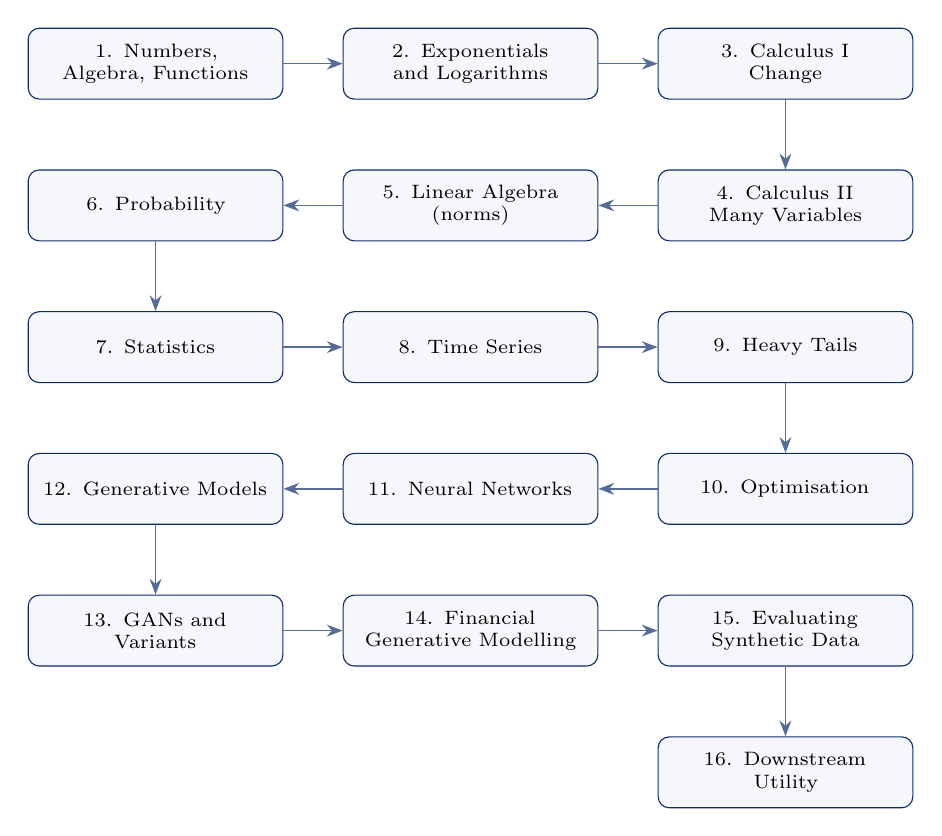
\begin{tikzpicture}[
  node/.style={rectangle, rounded corners=4pt, draw=Navy, fill=LBg,
               text width=3.0cm, align=center, minimum height=0.9cm, font=\scriptsize},
  todo/.style={rectangle, rounded corners=4pt, draw=Navy!35, fill=white,
               text width=3.0cm, align=center, minimum height=0.9cm,
               font=\scriptsize\itshape, dashed},
  arr/.style={-Stealth, semithick, draw=Navy!70}
]
\node[node] (c1) at (0,0)      {1. Numbers,\\Algebra, Functions};
\node[node] (c2) at (4,0)      {2. Exponentials\\and Logarithms};
\node[node] (c3) at (8,0)      {3. Calculus I\\Change};
\node[node] (c4) at (8,-1.8)   {4. Calculus II\\Many Variables};
\node[node] (c5) at (4,-1.8)   {5. Linear Algebra\\(norms)};
\node[node] (c6) at (0,-1.8)   {6. Probability};
\node[node] (c7) at (0,-3.6)   {7. Statistics};
\node[node] (c8) at (4,-3.6)   {8. Time Series};
\node[node] (c9) at (8,-3.6)   {9. Heavy Tails};
\node[node] (c10) at (8,-5.4)  {10. Optimisation};
\node[node] (c11) at (4,-5.4)  {11. Neural Networks};
\node[node] (c12) at (0,-5.4)  {12. Generative Models};
\node[node] (c13) at (0,-7.2)  {13. GANs and\\Variants};
\node[node] (c14) at (4,-7.2)  {14. Financial\\Generative Modelling};
\node[node] (c15) at (8,-7.2)  {15. Evaluating\\Synthetic Data};
\node[node] (c16) at (8,-9.0)  {16. Downstream\\Utility};

\draw[arr] (c1) -- (c2);
\draw[arr] (c2) -- (c3);
\draw[arr] (c3) -- (c4);
\draw[arr] (c4) -- (c5);
\draw[arr] (c5) -- (c6);
\draw[arr] (c6) -- (c7);
\draw[arr] (c7) -- (c8);
\draw[arr] (c8) -- (c9);
\draw[arr] (c9) -- (c10);
\draw[arr] (c10) -- (c11);
\draw[arr] (c11) -- (c12);
\draw[arr] (c12) -- (c13);
\draw[arr] (c13) -- (c14);
\draw[arr] (c14) -- (c15);
\draw[arr] (c15) -- (c16);
\end{tikzpicture}
\end{center}

\medskip
All sixteen chapters are written. The critical path this book exists to support
runs

\medskip
\begin{center}
derivative $\to$ partial derivative $\to$ gradient $\to$ norm $\to$
Lipschitz continuity $\to$ Wasserstein distance $\to$ WGAN $\to$ critic $\to$
gradient penalty,
\end{center}

\medskip
and Chapters~\ref{ch:calculus1}--\ref{ch:linalg} supply every link in it up to
and including the norm.

\end{document}
